%% ----------------------------------------------------------------
%% Thesis.tex -- MAIN FILE (the one that you compile with LaTeX)
%% ---------------------------------------------------------------- 

% Set up the document
\documentclass[a4paper, 11pt, oneside]{Thesis}  % Use the "Thesis" style, based on the ECS Thesis style by Steve Gunn
\graphicspath{{Figures/}}  % Location of the graphics files (set up for graphics to be in PDF format)

% Include any extra LaTeX packages required
\usepackage[square, numbers, comma, sort&compress]{natbib}  % Use the "Natbib" style for the references in the Bibliography
\usepackage{verbatim}  % Needed for the "comment" environment to make LaTeX comments
\usepackage{vector}  % Allows "\bvec{}" and "\buvec{}" for "blackboard" style bold vectors in maths
%\usepackage{subfloat}
%\usepackage{graphicx}
%\usepackage{caption}
\usepackage{subcaption}
\usepackage{multirow}
\usepackage{upgreek}
\usepackage{amsmath}
\usepackage{float}

\hypersetup{urlcolor=blue, colorlinks=true}  % Colours hyperlinks in blue, but this can be distracting if there are many links.

% List of LHCb aliases to save time
\newboolean{uprightparticles}
\setboolean{uprightparticles}{false} %Set to true to get roman particle symbols
%%% $Id: lhcb-symbols-def.tex 9171 2011-08-24 11:58:40Z spradlin $
%%% ======================================================================
%%% Purpose: standard LHCb aliases
%%% Author: Originally Ulrik Egede, adapted by Tomasz Skwarnicki for templates,
%%% rewritten by Chris Parkes
%%% Created on: 2009-09-24
%%% =======================================================================

%%% this has to go before \begin{document}
%%%\usepackage{ifthen} 
%%%\newboolean{uprightparticles}
%%%\setboolean{uprightparticles}{true} %Set to false to get italic particle symbols

%%% Add comments with at least three %%% preceding.
%%% Add new sections with one % preceding
%%% Add new subsections with two %% preceding

%%%%%%%%%%%%%
% Experiments
%%%%%%%%%%%%%
\def\lhcb {LHCb\xspace}
\def\LHCb {\lhcb}
\def\ux85 {UX85\xspace}
\def\cern {CERN\xspace}
\def\lhc {LHC\xspace}
\def\atlas {ATLAS\xspace}
\def\cms {CMS\xspace}
\def\alice {ALICE\xspace}
\def\babar  {BABAR\xspace}
\def\belle  {BELLE\xspace}
\def\aleph  {ALEPH\xspace}
\def\delphi {DELPHI\xspace}
\def\opal   {OPAL\xspace}
\def\lthree {L3\xspace}
\def\lep    {LEP\xspace}
\def\cdf    {CDF\xspace}
\def\dzero  {D0\xspace}
\def\sld    {SLD\xspace}
\def\cleo   {CLEO\xspace}
\def\uaone  {UA1\xspace}
\def\uatwo  {UA2\xspace}
\def\tevatron {TEVATRON\xspace}

%% LHCb sub-detectors and sub-systems

\def\pu     {PU\xspace}
\def\velo   {VELO\xspace}
\def\rich   {RICH\xspace}
\def\richone {RICH1\xspace}
\def\richtwo {RICH2\xspace}
\def\ttracker {TT\xspace}
\def\intr   {IT\xspace}
\def\st     {ST\xspace}
\def\ot     {OT\xspace}
\def\Tone   {T1\xspace}
\def\Ttwo   {T2\xspace}
\def\Tthree {T3\xspace}
\def\Mone   {M1\xspace}
\def\Mtwo   {M2\xspace}
\def\Mthree {M3\xspace}
\def\Mfour  {M4\xspace}
\def\Mfive  {M5\xspace}
\def\ecal   {ECAL\xspace}
\def\spd    {SPD\xspace}
\def\presh  {PS\xspace}
\def\hcal   {HCAL\xspace}
\def\bcm    {BCM\xspace}

\def\ode    {ODE\xspace}
\def\daq    {DAQ\xspace}
\def\tfc    {TFC\xspace}
\def\ecs    {ECS\xspace}
\def\lone   {L0\xspace}
\def\hlt    {HLT\xspace}
\def\hltone {HLT1\xspace}
\def\hlttwo {HLT2\xspace}

%%% Upright (not slanted) Particles

\ifthenelse{\boolean{uprightparticles}}%
{\def\Palpha      {\ensuremath{\upalpha}\xspace}
 \def\Pbeta       {\ensuremath{\upbeta}\xspace}
 \def\Pgamma      {\ensuremath{\upgamma}\xspace}                 
 \def\Pdelta      {\ensuremath{\updelta}\xspace}                 
 \def\Pepsilon    {\ensuremath{\upepsilon}\xspace}                 
 \def\Pvarepsilon {\ensuremath{\upvarepsilon}\xspace}                 
 \def\Pzeta       {\ensuremath{\upzeta}\xspace}                 
 \def\Peta        {\ensuremath{\upeta}\xspace}                 
 \def\Ptheta      {\ensuremath{\uptheta}\xspace}                 
 \def\Pvartheta   {\ensuremath{\upvartheta}\xspace}                 
 \def\Piota       {\ensuremath{\upiota}\xspace}                 
 \def\Pkappa      {\ensuremath{\upkappa}\xspace}                 
 \def\Plambda     {\ensuremath{\uplambda}\xspace}                 
 \def\Pmu         {\ensuremath{\upmu}\xspace}                 
 \def\Pnu         {\ensuremath{\upnu}\xspace}                 
 \def\Pxi         {\ensuremath{\upxi}\xspace}                 
 \def\Ppi         {\ensuremath{\uppi}\xspace}                 
 \def\Pvarpi      {\ensuremath{\upvarpi}\xspace}                 
 \def\Prho        {\ensuremath{\uprho}\xspace}                 
 \def\Pvarrho     {\ensuremath{\upvarrho}\xspace}                 
 \def\Ptau        {\ensuremath{\uptau}\xspace}                 
 \def\Pupsilon    {\ensuremath{\upupsilon}\xspace}                 
 \def\Pphi        {\ensuremath{\upphi}\xspace}                 
 \def\Pvarphi     {\ensuremath{\upvarphi}\xspace}                 
 \def\Pchi        {\ensuremath{\upchi}\xspace}                 
 \def\Ppsi        {\ensuremath{\uppsi}\xspace}                 
 \def\Pomega      {\ensuremath{\upomega}\xspace}                 

 \def\PDelta      {\ensuremath{\Delta}\xspace}                 
 \def\PXi      {\ensuremath{\Xi}\xspace}                 
 \def\PLambda      {\ensuremath{\Lambda}\xspace}                 
 \def\PSigma      {\ensuremath{\Sigma}\xspace}                 
 \def\POmega      {\ensuremath{\Omega}\xspace}                 
 \def\PUpsilon      {\ensuremath{\Upsilon}\xspace}                 
 
 %\mathchardef\Deltares="7101
 %\mathchardef\Xi="7104
 %\mathchardef\Lambda="7103
 %\mathchardef\Sigma="7106
 %\mathchardef\Omega="710A


 \def\PA      {\ensuremath{\mathrm{A}}\xspace}                 
 \def\PB      {\ensuremath{\mathrm{B}}\xspace}                 
 \def\PC      {\ensuremath{\mathrm{C}}\xspace}                 
 \def\PD      {\ensuremath{\mathrm{D}}\xspace}                 
 \def\PE      {\ensuremath{\mathrm{E}}\xspace}                 
 \def\PF      {\ensuremath{\mathrm{F}}\xspace}                 
 \def\PG      {\ensuremath{\mathrm{G}}\xspace}                 
 \def\PH      {\ensuremath{\mathrm{H}}\xspace}                 
 \def\PI      {\ensuremath{\mathrm{I}}\xspace}                 
 \def\PJ      {\ensuremath{\mathrm{J}}\xspace}                 
 \def\PK      {\ensuremath{\mathrm{K}}\xspace}                 
 \def\PL      {\ensuremath{\mathrm{L}}\xspace}                 
 \def\PM      {\ensuremath{\mathrm{M}}\xspace}                 
 \def\PN      {\ensuremath{\mathrm{N}}\xspace}                 
 \def\PO      {\ensuremath{\mathrm{O}}\xspace}                 
 \def\PP      {\ensuremath{\mathrm{P}}\xspace}                 
 \def\PQ      {\ensuremath{\mathrm{Q}}\xspace}                 
 \def\PR      {\ensuremath{\mathrm{R}}\xspace}                 
 \def\PS      {\ensuremath{\mathrm{S}}\xspace}                 
 \def\PT      {\ensuremath{\mathrm{T}}\xspace}                 
 \def\PU      {\ensuremath{\mathrm{U}}\xspace}                 
 \def\PV      {\ensuremath{\mathrm{V}}\xspace}                 
 \def\PW      {\ensuremath{\mathrm{W}}\xspace}                 
 \def\PX      {\ensuremath{\mathrm{X}}\xspace}                 
 \def\PY      {\ensuremath{\mathrm{Y}}\xspace}                 
 \def\PZ      {\ensuremath{\mathrm{Z}}\xspace}                 
 \def\Pa      {\ensuremath{\mathrm{a}}\xspace}                 
 \def\Pb      {\ensuremath{\mathrm{b}}\xspace}                 
 \def\Pc      {\ensuremath{\mathrm{c}}\xspace}                 
 \def\Pd      {\ensuremath{\mathrm{d}}\xspace}                 
 \def\Pe      {\ensuremath{\mathrm{e}}\xspace}                 
 \def\Pf      {\ensuremath{\mathrm{f}}\xspace}                 
 \def\Pg      {\ensuremath{\mathrm{g}}\xspace}                 
 \def\Ph      {\ensuremath{\mathrm{h}}\xspace}                 
 \def\Pi      {\ensuremath{\mathrm{i}}\xspace}                 
 \def\Pj      {\ensuremath{\mathrm{j}}\xspace}                 
 \def\Pk      {\ensuremath{\mathrm{k}}\xspace}                 
 \def\Pl      {\ensuremath{\mathrm{l}}\xspace}                 
 \def\Pm      {\ensuremath{\mathrm{m}}\xspace}                 
 \def\Pn      {\ensuremath{\mathrm{n}}\xspace}                 
 \def\Po      {\ensuremath{\mathrm{o}}\xspace}                 
 \def\Pp      {\ensuremath{\mathrm{p}}\xspace}                 
 \def\Pq      {\ensuremath{\mathrm{q}}\xspace}                 
 \def\Pr      {\ensuremath{\mathrm{r}}\xspace}                 
 \def\Ps      {\ensuremath{\mathrm{s}}\xspace}                 
 \def\Pt      {\ensuremath{\mathrm{t}}\xspace}                 
 \def\Pu      {\ensuremath{\mathrm{u}}\xspace}                 
 \def\Pv      {\ensuremath{\mathrm{v}}\xspace}                 
 \def\Pw      {\ensuremath{\mathrm{w}}\xspace}                 
 \def\Px      {\ensuremath{\mathrm{x}}\xspace}                 
 \def\Py      {\ensuremath{\mathrm{y}}\xspace}                 
 \def\Pz      {\ensuremath{\mathrm{z}}\xspace}                 
}
{\def\Palpha      {\ensuremath{\alpha}\xspace}
 \def\Pbeta       {\ensuremath{\beta}\xspace}
 \def\Pgamma      {\ensuremath{\gamma}\xspace}                 
 \def\Pdelta      {\ensuremath{\delta}\xspace}                 
 \def\Pepsilon    {\ensuremath{\epsilon}\xspace}                 
 \def\Pvarepsilon {\ensuremath{\varepsilon}\xspace}                 
 \def\Pzeta       {\ensuremath{\zeta}\xspace}                 
 \def\Peta        {\ensuremath{\eta}\xspace}                 
 \def\Ptheta      {\ensuremath{\theta}\xspace}                 
 \def\Pvartheta   {\ensuremath{\vartheta}\xspace}                 
 \def\Piota       {\ensuremath{\iota}\xspace}                 
 \def\Pkappa      {\ensuremath{\kappa}\xspace}                 
 \def\Plambda     {\ensuremath{\lambda}\xspace}                 
 \def\Pmu         {\ensuremath{\mu}\xspace}                 
 \def\Pnu         {\ensuremath{\nu}\xspace}                 
 \def\Pxi         {\ensuremath{\xi}\xspace}                 
 \def\Ppi         {\ensuremath{\pi}\xspace}                 
 \def\Pvarpi      {\ensuremath{\varpi}\xspace}                 
 \def\Prho        {\ensuremath{\rho}\xspace}                 
 \def\Pvarrho     {\ensuremath{\varrho}\xspace}                 
 \def\Ptau        {\ensuremath{\tau}\xspace}                 
 \def\Pupsilon    {\ensuremath{\upsilon}\xspace}                 
 \def\Pphi        {\ensuremath{\phi}\xspace}                 
 \def\Pvarphi     {\ensuremath{\varphi}\xspace}                 
 \def\Pchi        {\ensuremath{\chi}\xspace}                 
 \def\Ppsi        {\ensuremath{\psi}\xspace}                 
 \def\Pomega      {\ensuremath{\omega}\xspace}                 
 \mathchardef\PDelta="7101
 \mathchardef\PXi="7104
 \mathchardef\PLambda="7103
 \mathchardef\PSigma="7106
 \mathchardef\POmega="710A
 \mathchardef\PUpsilon="7107
 \def\PA      {\ensuremath{A}\xspace}                 
 \def\PB      {\ensuremath{B}\xspace}                 
 \def\PC      {\ensuremath{C}\xspace}                 
 \def\PD      {\ensuremath{D}\xspace}                 
 \def\PE      {\ensuremath{E}\xspace}                 
 \def\PF      {\ensuremath{F}\xspace}                 
 \def\PG      {\ensuremath{G}\xspace}                 
 \def\PH      {\ensuremath{H}\xspace}                 
 \def\PI      {\ensuremath{I}\xspace}                 
 \def\PJ      {\ensuremath{J}\xspace}                 
 \def\PK      {\ensuremath{K}\xspace}                 
 \def\PL      {\ensuremath{L}\xspace}                 
 \def\PM      {\ensuremath{M}\xspace}                 
 \def\PN      {\ensuremath{N}\xspace}                 
 \def\PO      {\ensuremath{O}\xspace}                 
 \def\PP      {\ensuremath{P}\xspace}                 
 \def\PQ      {\ensuremath{Q}\xspace}                 
 \def\PR      {\ensuremath{R}\xspace}                 
 \def\PS      {\ensuremath{S}\xspace}                 
 \def\PT      {\ensuremath{T}\xspace}                 
 \def\PU      {\ensuremath{U}\xspace}                 
 \def\PV      {\ensuremath{V}\xspace}                 
 \def\PW      {\ensuremath{W}\xspace}                 
 \def\PX      {\ensuremath{X}\xspace}                 
 \def\PY      {\ensuremath{Y}\xspace}                 
 \def\PZ      {\ensuremath{Z}\xspace}                 
 \def\Pa      {\ensuremath{a}\xspace}                 
 \def\Pb      {\ensuremath{b}\xspace}                 
 \def\Pc      {\ensuremath{c}\xspace}                 
 \def\Pd      {\ensuremath{d}\xspace}                 
 \def\Pe      {\ensuremath{e}\xspace}                 
 \def\Pf      {\ensuremath{f}\xspace}                 
 \def\Pg      {\ensuremath{g}\xspace}                 
 \def\Ph      {\ensuremath{h}\xspace}                 
 \def\Pi      {\ensuremath{i}\xspace}                 
 \def\Pj      {\ensuremath{j}\xspace}                 
 \def\Pk      {\ensuremath{k}\xspace}                 
 \def\Pl      {\ensuremath{l}\xspace}                 
 \def\Pm      {\ensuremath{m}\xspace}                 
 \def\Pn      {\ensuremath{n}\xspace}                 
 \def\Po      {\ensuremath{o}\xspace}                 
 \def\Pp      {\ensuremath{p}\xspace}                 
 \def\Pq      {\ensuremath{q}\xspace}                 
 \def\Pr      {\ensuremath{r}\xspace}                 
 \def\Ps      {\ensuremath{s}\xspace}                 
 \def\Pt      {\ensuremath{t}\xspace}                 
 \def\Pu      {\ensuremath{u}\xspace}                 
 \def\Pv      {\ensuremath{v}\xspace}                 
 \def\Pw      {\ensuremath{w}\xspace}                 
 \def\Px      {\ensuremath{x}\xspace}                 
 \def\Py      {\ensuremath{y}\xspace}                 
 \def\Pz      {\ensuremath{z}\xspace}                 
}

%%%%%%%%%%%%%%%%%%%%%%%%%%%%%%%%%%%%%%%%%%%%%%%
% Particles

%% Leptons

\let\emi\en
\def\electron   {\ensuremath{\Pe}\xspace}
\def\en         {\ensuremath{\Pe^-}\xspace}   % electron negative (\em is taken)
\def\ep         {\ensuremath{\Pe^+}\xspace}
\def\epm        {\ensuremath{\Pe^\pm}\xspace} 
\def\epem       {\ensuremath{\Pe^+\Pe^-}\xspace}
\def\ee         {\ensuremath{\Pe^-\Pe^-}\xspace}

\def\mmu        {\ensuremath{\Pmu}\xspace}
\def\mup        {\ensuremath{\Pmu^+}\xspace}
\def\mun        {\ensuremath{\Pmu^-}\xspace} % muon negative (\mum is taken)
\def\mumu       {\ensuremath{\Pmu^+\Pmu^-}\xspace}
\def\mtau       {\ensuremath{\Ptau}\xspace}

\def\taup       {\ensuremath{\Ptau^+}\xspace}
\def\taum       {\ensuremath{\Ptau^-}\xspace}
\def\tautau     {\ensuremath{\Ptau^+\Ptau^-}\xspace}

\def\ellm       {\ensuremath{\ell^-}\xspace}
\def\ellp       {\ensuremath{\ell^+}\xspace}
\def\ellell     {\ensuremath{\ell^+ \ell^-}\xspace}

\def\neu        {\ensuremath{\Pnu}\xspace}
\def\neub       {\ensuremath{\overline{\Pnu}}\xspace}
\def\nuenueb    {\ensuremath{\neu\neub}\xspace}
\def\neue       {\ensuremath{\neu_e}\xspace}
\def\neueb      {\ensuremath{\neub_e}\xspace}
\def\neueneueb  {\ensuremath{\neue\neueb}\xspace}
\def\neum       {\ensuremath{\neu_\mu}\xspace}
\def\neumb      {\ensuremath{\neub_\mu}\xspace}
\def\neumneumb  {\ensuremath{\neum\neumb}\xspace}
\def\neut       {\ensuremath{\neu_\tau}\xspace}
\def\neutb      {\ensuremath{\neub_\tau}\xspace}
\def\neutneutb  {\ensuremath{\neut\neutb}\xspace}
\def\neul       {\ensuremath{\neu_\ell}\xspace}
\def\neulb      {\ensuremath{\neub_\ell}\xspace}
\def\neulneulb  {\ensuremath{\neul\neulb}\xspace}

%% Gauge bosons and scalars

\def\g      {\ensuremath{\Pgamma}\xspace}
\def\H      {\ensuremath{\PH^0}\xspace}
\def\Hp     {\ensuremath{\PH^+}\xspace}
\def\Hm     {\ensuremath{\PH^-}\xspace}
\def\Hpm    {\ensuremath{\PH^\pm}\xspace}
\def\W      {\ensuremath{\PW}\xspace}
\def\Wp     {\ensuremath{\PW^+}\xspace}
\def\Wm     {\ensuremath{\PW^-}\xspace}
\def\Wpm    {\ensuremath{\PW^\pm}\xspace}
\def\Z      {\ensuremath{\PZ^0}\xspace}

%% Quarks

\def\q     {\ensuremath{\Pq}\xspace}
\def\qbar  {\ensuremath{\overline \q}\xspace}
\def\qqbar {\ensuremath{\q\qbar}\xspace}
\def\u     {\ensuremath{\Pu}\xspace}
\def\ubar  {\ensuremath{\overline \u}\xspace}
\def\uubar {\ensuremath{\u\ubar}\xspace}
\def\d     {\ensuremath{\Pd}\xspace}
\def\dbar  {\ensuremath{\overline \d}\xspace}
\def\ddbar {\ensuremath{\d\dbar}\xspace}
\def\s     {\ensuremath{\Ps}\xspace}
\def\sbar  {\ensuremath{\overline \s}\xspace}
\def\ssbar {\ensuremath{\s\sbar}\xspace}
\def\c     {\ensuremath{\Pc}\xspace}
\def\cbar  {\ensuremath{\overline \c}\xspace}
\def\ccbar {\ensuremath{\c\cbar}\xspace}
\def\b     {\ensuremath{\Pb}\xspace}
\def\bbar  {\ensuremath{\overline \b}\xspace}
\def\bbbar {\ensuremath{\b\bbar}\xspace}
\def\t     {\ensuremath{\Pt}\xspace}
\def\tbar  {\ensuremath{\overline \t}\xspace}
\def\ttbar {\ensuremath{\t\tbar}\xspace}

%% Light mesons

\def\pion  {\ensuremath{\Ppi}\xspace}
\def\piz   {\ensuremath{\pion^0}\xspace}
\def\pizs  {\ensuremath{\pion^0\mbox\,\rm{s}}\xspace}
\def\ppz   {\ensuremath{\pion^0\pion^0}\xspace}
\def\pip   {\ensuremath{\pion^+}\xspace}
\def\pim   {\ensuremath{\pion^-}\xspace}
\def\pipi  {\ensuremath{\pion^+\pion^-}\xspace}
\def\pipm  {\ensuremath{\pion^\pm}\xspace}
\def\pimp  {\ensuremath{\pion^\mp}\xspace}

\def\kaon  {\ensuremath{\PK}\xspace}
%%% do NOT use ensuremath here
  \def\Kbar  {\kern 0.2em\overline{\kern -0.2em \PK}{}\xspace}
\def\Kb    {\ensuremath{\Kbar}\xspace}
\def\Kz    {\ensuremath{\kaon^0}\xspace}
\def\Kzb   {\ensuremath{\Kbar^0}\xspace}
\def\KzKzb {\ensuremath{\Kz \kern -0.16em \Kzb}\xspace}
\def\Kp    {\ensuremath{\kaon^+}\xspace}
\def\Km    {\ensuremath{\kaon^-}\xspace}
\def\Kpm   {\ensuremath{\kaon^\pm}\xspace}
\def\Kmp   {\ensuremath{\kaon^\mp}\xspace}
\def\KpKm  {\ensuremath{\Kp \kern -0.16em \Km}\xspace}
\def\KS    {\ensuremath{\kaon^0_{\rm\scriptscriptstyle S}}\xspace} 
\def\KL    {\ensuremath{\kaon^0_{\rm\scriptscriptstyle L}}\xspace} 
\def\Kstarz  {\ensuremath{\kaon^{*0}}\xspace}
\def\Kstarzb {\ensuremath{\Kbar^{*0}}\xspace}
\def\Kstar   {\ensuremath{\kaon^*}\xspace}
\def\Kstarb  {\ensuremath{\Kbar^*}\xspace}
\def\Kstarp  {\ensuremath{\kaon^{*+}}\xspace}
\def\Kstarm  {\ensuremath{\kaon^{*-}}\xspace}
\def\Kstarpm {\ensuremath{\kaon^{*\pm}}\xspace}
\def\Kstarmp {\ensuremath{\kaon^{*\mp}}\xspace}

\newcommand{\etapr}{\ensuremath{\Peta^{\prime}}\xspace}

%% Heavy mesons

%%% do NOT use ensuremath here
  \def\Dbar    {\kern 0.2em\overline{\kern -0.2em \PD}{}\xspace}
\def\D       {\ensuremath{\PD}\xspace}
\def\Db      {\ensuremath{\Dbar}\xspace}
\def\Dz      {\ensuremath{\D^0}\xspace}
\def\Dzb     {\ensuremath{\Dbar^0}\xspace}
\def\DzDzb   {\ensuremath{\Dz {\kern -0.16em \Dzb}}\xspace}
\def\Dp      {\ensuremath{\D^+}\xspace}
\def\Dm      {\ensuremath{\D^-}\xspace}
\def\Dpm     {\ensuremath{\D^\pm}\xspace}
\def\Dmp     {\ensuremath{\D^\mp}\xspace}
\def\DpDm    {\ensuremath{\Dp {\kern -0.16em \Dm}}\xspace}
\def\Dstar   {\ensuremath{\D^*}\xspace}
\def\Dstarb  {\ensuremath{\Dbar^*}\xspace}
\def\Dstarz  {\ensuremath{\D^{*0}}\xspace}
\def\Dstarzb {\ensuremath{\Dbar^{*0}}\xspace}
\def\Dstarp  {\ensuremath{\D^{*+}}\xspace}
\def\Dstarm  {\ensuremath{\D^{*-}}\xspace}
\def\Dstarpm {\ensuremath{\D^{*\pm}}\xspace}
\def\Dstarmp {\ensuremath{\D^{*\mp}}\xspace}
\def\Ds      {\ensuremath{\D^+_s}\xspace}
\def\Dsp     {\Ds}
\def\Dsm     {\ensuremath{\D^-_s}\xspace}
\def\Dspm    {\ensuremath{\D^{\pm}_s}\xspace}
\def\Dsmp    {\ensuremath{\D^{\mp}_s}\xspace}
\def\Dsb     {\ensuremath{\Dbar^+_s}\xspace}
\def\Dss     {\ensuremath{\D^{*+}_s}\xspace}

\def\Dpors      {\ensuremath{\D^+_{(s)}}\xspace}

\def\B       {\ensuremath{\PB}\xspace}
%%% do NOT use ensuremath here
  \def\Bbar    {\kern 0.18em\overline{\kern -0.18em \PB}{}\xspace}
\def\Bb      {\ensuremath{\Bbar}\xspace}
\def\BBbar   {\ensuremath{\B\Bbar}\xspace} 
\def\Bz      {\ensuremath{\B^0}\xspace}
\def\Bzb     {\ensuremath{\Bbar^0}\xspace}
\def\Bu      {\ensuremath{\B^+}\xspace}
\def\Bub     {\ensuremath{\B^-}\xspace}
\def\Bp      {\ensuremath{\Bu}\xspace}
\def\Bm      {\ensuremath{\Bub}\xspace}
\def\Bpm     {\ensuremath{\B^\pm}\xspace}
\def\Bmp     {\ensuremath{\B^\mp}\xspace}
\def\Bd      {\ensuremath{\B^0}\xspace}
\def\Bs      {\ensuremath{\B^0_s}\xspace}
\def\Bsb     {\ensuremath{\Bbar^0_s}\xspace}
\def\Bdb     {\ensuremath{\Bbar^0}\xspace}
\def\Bc      {\ensuremath{\B_c^+}\xspace}
\def\Bcb     {\ensuremath{\B_c^-}\xspace}

%% Onia

\def\jpsi     {\ensuremath{{\PJ\mskip -3mu/\mskip -2mu\Ppsi\mskip 2mu}}\xspace}
\def\psitwos  {\ensuremath{\Ppsi{(2S)}}\xspace}
\def\psiprpr  {\ensuremath{\Ppsi(3770)}\xspace}
\def\etac     {\ensuremath{\Peta_c}\xspace}
\def\chiczero {\ensuremath{\Pchi_{c0}}\xspace}
\def\chicone  {\ensuremath{\Pchi_{c1}}\xspace}
\def\chictwo  {\ensuremath{\Pchi_{c2}}\xspace}
  %\mathchardef\Upsilon="7107
  \def\Y#1S{\ensuremath{\PUpsilon{(#1S)}}\xspace}% no space before {...}!
\def\OneS  {\Y1S}
\def\TwoS  {\Y2S}
\def\ThreeS{\Y3S}
\def\FourS {\Y4S}
\def\FiveS {\Y5S}

\def\chic  {\ensuremath{\Pchi_{c}}\xspace}

%% Baryons

\def\proton      {\ensuremath{\Pp}\xspace}
\def\antiproton  {\ensuremath{\overline \proton}\xspace}
\def\neutron     {\ensuremath{\Pn}\xspace}
\def\antineutron {\ensuremath{\overline \neutron}\xspace}

\def\Deltares {\ensuremath{\PDelta}\xspace}
\def\Deltaresbar{\ensuremath{\overline \Deltares}\xspace}
\def\Xires {\ensuremath{\PXi}\xspace}
\def\Xiresbar{\ensuremath{\overline \Xires}\xspace}
\def\L {\ensuremath{\PLambda}\xspace}
\def\Lbar{\ensuremath{\overline \L}\xspace}
\def\Lambdares {\ensuremath{\PLambda}\xspace}
\def\Lambdaresbar{\ensuremath{\overline \Lambdares}\xspace}
\def\Sigmares {\ensuremath{\PSigma}\xspace}
\def\Sigmaresbar{\ensuremath{\overline \Sigmares}\xspace}
\def\Omegares {\ensuremath{\POmega}\xspace}
\def\Omegaresbar{\ensuremath{\overline \Omegares}\xspace}
\def\Lambdacp{\ensuremath{\PLambda_c^+}\xspace}
\def\Lambdacm{\ensuremath{\PLambda_c^-}\xspace}
\def\Lambdacpm{\ensuremath{\PLambda_c^{\pm}\xspace}}
\def\Lambdacmp{\ensuremath{\PLambda_c^{\mp}\xspace}}

%%% do NOT use ensuremath here
 % \def\Deltabar{\kern 0.25em\overline{\kern -0.25em \Deltares}{}\xspace}
 % \def\Lbar{\kern 0.2em\overline{\kern -0.2em\Lambda\kern 0.05em}\kern-0.05em{}\xspace}
 % \def\Sigbar{\kern 0.2em\overline{\kern -0.2em \Sigma}{}\xspace}
 % \def\Xibar{\kern 0.2em\overline{\kern -0.2em \Xi}{}\xspace}
 % \def\Obar{\kern 0.2em\overline{\kern -0.2em \Omega}{}\xspace}
 % \def\Nbar{\kern 0.2em\overline{\kern -0.2em N}{}\xspace}
 % \def\Xb{\kern 0.2em\overline{\kern -0.2em X}{}\xspace}

\def\Lb      {\ensuremath{\L_b}\xspace}
\def\Lbbar   {\ensuremath{\Lbar_b}\xspace}
\def\Lc      {\ensuremath{\L_c}\xspace}
\def\Lcp      {\ensuremath{\L_c^+}\xspace}
\def\Lcm      {\ensuremath{\L_c^-}\xspace}
\def\Lcpm      {\ensuremath{\L_c^{\pm}}\xspace}
\def\Lcmp      {\ensuremath{\L_c^{\mp}}\xspace}
%\def\Lcbar   {\ensuremath{\Lbar_c}\xspace}

%%%%%%%%%%%%%%%%%%
% Physics symbols
%%%%%%%%%%%%%%%%%

%% Decays
\def\BR         {{\ensuremath{\cal B}\xspace}}
\def\BRvis      {{\ensuremath{\BR_{\rm{vis}}}}}
\newcommand{\decay}[2]{\ensuremath{#1\!\to #2}\xspace}         % {\Pa}{\Pb \Pc}
\def\ra                 {\ensuremath{\rightarrow}\xspace}
\def\to                 {\ensuremath{\rightarrow}\xspace}

%% Lifetimes
\newcommand{\tauBs}{\ensuremath{\tau_{\Bs}}\xspace}
\newcommand{\tauBd}{\ensuremath{\tau_{\B}}\xspace}
\newcommand{\tauBz}{\ensuremath{\tau_{\B}}\xspace}
\newcommand{\tauBu}{\ensuremath{\tau_{\Bp}}\xspace}
\newcommand{\tauDp}{\ensuremath{\tau_{\Dp}}\xspace}
\newcommand{\tauDz}{\ensuremath{\tau_{\Dz}}\xspace}
\newcommand{\tauL}{\ensuremath{\tau_{\rm L}}\xspace}
\newcommand{\tauH}{\ensuremath{\tau_{\rm H}}\xspace}

%% Masses
\newcommand{\mBd}{\ensuremath{m_{\Bd}}\xspace}
\newcommand{\mBp}{\ensuremath{m_{\Bp}}\xspace}
\newcommand{\mBs}{\ensuremath{m_{\Bs}}\xspace}
\newcommand{\mBc}{\ensuremath{m_{\Bc}}\xspace}
\newcommand{\mLb}{\ensuremath{m_{\Lb}}\xspace}

%% EW theory, groups
\def\grpsuthree {\ensuremath{\mathrm{SU}(3)}\xspace}
\def\grpsutwo    {\ensuremath{\mathrm{SU}(2)}\xspace}
\def\grpuone    {\ensuremath{\mathrm{U}(1)}\xspace}

\def\ssqtw {\ensuremath{\sin^{2}\!\theta_{\mathrm{W}}}\xspace}
\def\csqtw {\ensuremath{\cos^{2}\!\theta_{\mathrm{W}}}\xspace}
\def\stw   {\ensuremath{\sin\theta_{\mathrm{W}}}\xspace}
\def\ctw   {\ensuremath{\cos\theta_{\mathrm{W}}}\xspace}
\def\ssqtwef {\ensuremath{{\sin}^{2}\theta_{\mathrm{W}}^{\mathrm{eff}}}\xspace}
\def\csqtwef {\ensuremath{{\cos}^{2}\theta_{\mathrm{W}}^{\mathrm{eff}}}\xspace}
\def\stwef {\ensuremath{\sin\theta_{\mathrm{W}}^{\mathrm{eff}}}\xspace}
\def\ctwef {\ensuremath{\cos\theta_{\mathrm{W}}^{\mathrm{eff}}}\xspace}
\def\gv    {\ensuremath{g_{\mbox{\tiny V}}}\xspace}
\def\ga    {\ensuremath{g_{\mbox{\tiny A}}}\xspace}

\def\order   {\ensuremath{\mathcal{O}}\xspace}
\def\ordalph {\ensuremath{\mathcal{O}(\alpha)}\xspace}
\def\ordalsq {\ensuremath{\mathcal{O}(\alpha^{2})}\xspace}
\def\ordalcb {\ensuremath{\mathcal{O}(\alpha^{3})}\xspace}

%% QCD parameters
\newcommand{\as}{\ensuremath{\alpha_{\scriptscriptstyle S}}\xspace}
\newcommand{\MSb}{\ensuremath{\overline{\mathrm{MS}}}\xspace}
\newcommand{\lqcd}{\ensuremath{\Lambda_{\mathrm{QCD}}}\xspace}
\def\qsq       {\ensuremath{q^2}\xspace}

%% CKM, CP violation

\def\eps   {\ensuremath{\varepsilon}\xspace}
\def\epsK  {\ensuremath{\varepsilon_K}\xspace}
\def\epsB  {\ensuremath{\varepsilon_B}\xspace}
\def\epsp  {\ensuremath{\varepsilon^\prime_K}\xspace}

\def\CP                {\ensuremath{C\!P}\xspace}
\def\CPT               {\ensuremath{C\!PT}\xspace}

\def\rhobar {\ensuremath{\overline \rho}\xspace}
\def\etabar {\ensuremath{\overline \eta}\xspace}

\def\Vud  {\ensuremath{|V_{ud}|}\xspace}
\def\Vcd  {\ensuremath{|V_{cd}|}\xspace}
\def\Vtd  {\ensuremath{|V_{td}|}\xspace}
\def\Vus  {\ensuremath{|V_{us}|}\xspace}
\def\Vcs  {\ensuremath{|V_{cs}|}\xspace}
\def\Vts  {\ensuremath{|V_{ts}|}\xspace}
\def\Vub  {\ensuremath{|V_{ub}|}\xspace}
\def\Vcb  {\ensuremath{|V_{cb}|}\xspace}
\def\Vtb  {\ensuremath{|V_{tb}|}\xspace}

%% Oscillations

\newcommand{\dm}{\ensuremath{\Delta m}\xspace}
\newcommand{\dms}{\ensuremath{\Delta m_{\s}}\xspace}
\newcommand{\dmd}{\ensuremath{\Delta m_{\d}}\xspace}
\newcommand{\DG}{\ensuremath{\Delta\Gamma}\xspace}
\newcommand{\DGs}{\ensuremath{\Delta\Gamma_{\s}}\xspace}
\newcommand{\DGd}{\ensuremath{\Delta\Gamma_{\d}}\xspace}
\newcommand{\Gs}{\ensuremath{\Gamma_{\s}}\xspace}
\newcommand{\Gd}{\ensuremath{\Gamma_{\d}}\xspace}

\newcommand{\MBq}{\ensuremath{M_{\B_\q}}\xspace}
\newcommand{\DGq}{\ensuremath{\Delta\Gamma_{\q}}\xspace}
\newcommand{\Gq}{\ensuremath{\Gamma_{\q}}\xspace}
\newcommand{\dmq}{\ensuremath{\Delta m_{\q}}\xspace}
\newcommand{\GL}{\ensuremath{\Gamma_{\rm L}}\xspace}
\newcommand{\GH}{\ensuremath{\Gamma_{\rm H}}\xspace}

\newcommand{\DGsGs}{\ensuremath{\Delta\Gamma_{\s}/\Gamma_{\s}}\xspace}
\newcommand{\Delm}{\ensuremath{\Delta m}\xspace}
\newcommand{\ACP}{\ensuremath{{\cal A}^{\rm CP}}\xspace}
\newcommand{\Adir}{\ensuremath{{\cal A}^{\rm dir}}\xspace}
\newcommand{\Amix}{\ensuremath{{\cal A}^{\rm mix}}\xspace}
\newcommand{\ADelta}{\ensuremath{{\cal A}^\Delta}\xspace}
\newcommand{\phid}{\ensuremath{\phi_{\d}}\xspace}
\newcommand{\sinphid}{\ensuremath{\sin\!\phid}\xspace}
\newcommand{\phis}{\ensuremath{\phi_{\s}}\xspace}
\newcommand{\betas}{\ensuremath{\beta_{\s}}\xspace}
\newcommand{\sbetas}{\ensuremath{\sigma(\beta_{\s})}\xspace}
\newcommand{\stbetas}{\ensuremath{\sigma(2\beta_{\s})}\xspace}
\newcommand{\stphis}{\ensuremath{\sigma(\phi_{\s})}\xspace}
\newcommand{\sinphis}{\ensuremath{\sin\!\phis}\xspace}

%% Tagging
\newcommand{\edet}{{\ensuremath{\varepsilon_{\rm det}}}\xspace}
\newcommand{\erec}{{\ensuremath{\varepsilon_{\rm rec/det}}}\xspace}
\newcommand{\esel}{{\ensuremath{\varepsilon_{\rm sel/rec}}}\xspace}
\newcommand{\etrg}{{\ensuremath{\varepsilon_{\rm trg/sel}}}\xspace}
\newcommand{\etot}{{\ensuremath{\varepsilon_{\rm tot}}}\xspace}

\newcommand{\mistag}{\ensuremath{\omega}\xspace}
\newcommand{\wcomb}{\ensuremath{\omega^{\rm comb}}\xspace}
\newcommand{\etag}{{\ensuremath{\varepsilon_{\rm tag}}}\xspace}
\newcommand{\etagcomb}{{\ensuremath{\varepsilon_{\rm tag}^{\rm comb}}}\xspace}
\newcommand{\effeff}{\ensuremath{\varepsilon_{\rm eff}}\xspace}
\newcommand{\effeffcomb}{\ensuremath{\varepsilon_{\rm eff}^{\rm comb}}\xspace}
\newcommand{\efftag}{{\ensuremath{\etag(1-2\omega)^2}}\xspace}
\newcommand{\effD}{{\ensuremath{\etag D^2}}\xspace}

\newcommand{\etagprompt}{{\ensuremath{\varepsilon_{\rm tag}^{\rm Pr}}}\xspace}
\newcommand{\etagLL}{{\ensuremath{\varepsilon_{\rm tag}^{\rm LL}}}\xspace}

%% Key decay channels

\def\BdToKstmm    {\decay{\Bd}{\Kstarz\mup\mun}\xspace}
\def\BdbToKstmm   {\decay{\Bdb}{\Kstarzb\mup\mun}\xspace}

\def\BsToJPsiPhi  {\decay{\Bs}{\jpsi\phi}\xspace}
\def\BdToJPsiKst  {\decay{\Bd}{\jpsi\Kstarz}\xspace}
\def\BdbToJPsiKst {\decay{\Bdb}{\jpsi\Kstarzb}\xspace}

\def\BsPhiGam     {\decay{\Bd}{\phi \g}\xspace}
\def\BdKstGam     {\decay{\Bd}{\Kstarz \g}\xspace}

\def\BTohh        {\decay{\B}{\Ph^+ \Ph^-}\xspace}
\def\BdTopipi     {\decay{\Bd}{\pip\pim}\xspace}
\def\BdToKpi      {\decay{\Bd}{\Kp\pim}\xspace}
\def\BsToKK       {\decay{\Bs}{\Kp\Km}\xspace}
\def\BsTopiK      {\decay{\Bs}{\pip\Km}\xspace}

%% Rare decays
\def\BdKstee  {\decay{\Bd}{\Kstarz\epem}\xspace}
\def\BdbKstee {\decay{\Bdb}{\Kstarzb\epem}\xspace}
\def\bsll     {\decay{\b}{\s \ell^+ \ell^-}\xspace}
\def\AFB      {\ensuremath{A_{\mathrm{FB}}}\xspace}
\def\AT#1     {\ensuremath{A_T^{#1}}\xspace}           % 2
\def\btosgam  {\decay{\b}{\s \g}\xspace}
\def\btodgam  {\decay{\b}{\d \g}\xspace}
\def\Bsmm     {\decay{\Bs}{\mup\mun}\xspace}
\def\Bdmm     {\decay{\Bd}{\mup\mun}\xspace}
\def\ctl       {\ensuremath{\cos{\theta_l}}\xspace}
\def\ctk       {\ensuremath{\cos{\theta_K}}\xspace}

%% Wilson coefficients and operators
\def\C#1      {\ensuremath{\mathcal{C}_{#1}}\xspace}                       % 9
\def\Cp#1     {\ensuremath{\mathcal{C}_{#1}^{'}}\xspace}                    % 7
\def\Ceff#1   {\ensuremath{\mathcal{C}_{#1}^{\mathrm{(eff)}}}\xspace}        % 9  
\def\Cpeff#1  {\ensuremath{\mathcal{C}_{#1}^{'\mathrm{(eff)}}}\xspace}       % 7
\def\Ope#1    {\ensuremath{\mathcal{O}_{#1}}\xspace}                       % 2
\def\Opep#1   {\ensuremath{\mathcal{O}_{#1}^{'}}\xspace}                    % 7

%% Charm

\def\xprime     {\ensuremath{x^{\prime}}\xspace}
\def\yprime     {\ensuremath{y^{\prime}}\xspace}
\def\ycp        {\ensuremath{y_{CP}}\xspace}
\def\agamma     {\ensuremath{A_{\Gamma}}\xspace}
\def\kpi        {\ensuremath{\PK\Ppi}\xspace}
\def\kk         {\ensuremath{\PK\PK}\xspace}
\def\dkpi       {\decay{\PD}{\PK\Ppi}\xspace}
\def\dkk        {\decay{\PD}{\PK\PK}\xspace}
\def\dkpicf     {\decay{\Dz}{\Km\pip}\xspace}

%% QM
\newcommand{\bra}[1]{\ensuremath{\langle #1|}}             % {a}
\newcommand{\ket}[1]{\ensuremath{|#1\rangle}}              % {b}
\newcommand{\braket}[2]{\ensuremath{\langle #1|#2\rangle}} % {a}{b}

%%%%%%%%%%%%%%%%%%%%%%%%%%%%%%%%%%%%%%%%%%%%%%%%%%
% Units
%%%%%%%%%%%%%%%%%%%%%%%%%%%%%%%%%%%%%%%%%%%%%%%%%%
\newcommand{\unit}[1]{\ensuremath{\rm\,#1}\xspace}          % {kg}

%% Energy and momentum
\newcommand{\tev}{\ensuremath{\mathrm{\,Te\kern -0.1em V}}\xspace}
\newcommand{\gev}{\ensuremath{\mathrm{\,Ge\kern -0.1em V}}\xspace}
\newcommand{\mev}{\ensuremath{\mathrm{\,Me\kern -0.1em V}}\xspace}
\newcommand{\kev}{\ensuremath{\mathrm{\,ke\kern -0.1em V}}\xspace}
\newcommand{\ev}{\ensuremath{\mathrm{\,e\kern -0.1em V}}\xspace}
\newcommand{\tevc}{\ensuremath{{\mathrm{\tev\!/}c}}\xspace}
\newcommand{\gevc}{\ensuremath{{\mathrm{\gev\!/}c}}\xspace}
\newcommand{\mevc}{\ensuremath{{\mathrm{\mev\!/}c}}\xspace}
\newcommand{\tevcc}{\ensuremath{{\mathrm{\tev\!/}c^2}}\xspace}
\newcommand{\gevcc}{\ensuremath{{\mathrm{\gev\!/}c^2}}\xspace}
\newcommand{\mevcc}{\ensuremath{{\mathrm{\mev\!/}c^2}}\xspace}
\newcommand{\gevgevcccc}{\ensuremath{{\mathrm{\gev^2\!/}c^4}}\xspace}
\newcommand{\TeV}{\tev}
\newcommand{\GeV}{\gev}
\newcommand{\MeV}{\mev}
\newcommand{\KeV}{\kev}
\newcommand{\eV}{\ev}
\newcommand{\TeVc}{\tevc}
\newcommand{\GeVc}{\gevc}
\newcommand{\MeVc}{\mevc}
\newcommand{\TeVcc}{\tevcc}
\newcommand{\GeVcc}{\gevcc}
\newcommand{\MeVcc}{\mevcc}
\newcommand{\GeVGeVcccc}{\gevgevcccc}


%% Distance and area
\def\km   {\ensuremath{\rm \,km}\xspace}
\def\m    {\ensuremath{\rm \,m}\xspace}
\def\cm   {\ensuremath{\rm \,cm}\xspace}
\def\cma  {\ensuremath{{\rm \,cm}^2}\xspace}
\def\mm   {\ensuremath{\rm \,mm}\xspace}
\def\mma  {\ensuremath{\mm^2}\xspace}
\def\mum  {\ensuremath{\,\upmu\rm m}\xspace}
\def\muma {\ensuremath{\,\upmu\rm m^2}\xspace}
\def\nm   {\ensuremath{\rm \,nm}\xspace}
\def\fm   {\ensuremath{\rm \,fm}\xspace}
\def\barn{\ensuremath{\rm \,b}\xspace}
\def\barnhyph{\ensuremath{\rm -b}\xspace}
\def\mbarn{\ensuremath{\rm \,mb}\xspace}
\def\mub{\ensuremath{\rm \,\upmu b}\xspace}
\def\mbarnhyph{\ensuremath{\rm -mb}\xspace}
\def\nb {\ensuremath{\rm \,nb}\xspace}
\def\invnb {\ensuremath{\mbox{\,nb}^{-1}}\xspace}
\def\pb {\ensuremath{\rm \,pb}\xspace}
\def\invpb {\ensuremath{\mbox{\,pb}^{-1}}\xspace}
\def\fb   {\ensuremath{\mbox{\,fb}}\xspace}
\def\invfb   {\ensuremath{\mbox{\,fb}^{-1}}\xspace}

%% Time 
\def\sec  {\ensuremath{\rm {\,s}}\xspace}
\def\ms   {\ensuremath{{\rm \,ms}}\xspace}
\def\mus  {\ensuremath{\,\upmu{\rm s}}\xspace}
\def\ns   {\ensuremath{{\rm \,ns}}\xspace}
\def\ps   {\ensuremath{{\rm \,ps}}\xspace}
\def\fs   {\ensuremath{\rm \,fs}\xspace}

\def\mhz  {\ensuremath{{\rm \,MHz}}\xspace}
\def\khz  {\ensuremath{{\rm \,kHz}}\xspace}
\def\hz   {\ensuremath{{\rm \,Hz}}\xspace}

\def\invps{\ensuremath{{\rm \,ps^{-1}}}\xspace}

\def\yr   {\ensuremath{\rm \,yr}\xspace}
\def\hr   {\ensuremath{\rm \,hr}\xspace}

%% Temperature
\def\degc {\ensuremath{^\circ}{\rm \,C}\xspace}
\def\degk {\ensuremath {\rm K}\xspace}

%% Material lengths, radiation
\def\Xrad {\ensuremath{X_0}\xspace}
\def\NIL{\ensuremath{\lambda_{int}}\xspace}
\def\mip {MIP\xspace}
\def\neutroneq {\ensuremath{\rm \,n_{eq}}\xspace}
\def\neqcmcm {\ensuremath{\rm \,n_{eq} / cm^2}\xspace}
\def\kRad {\ensuremath{\rm \,kRad}\xspace}
\def\MRad {\ensuremath{\rm \,MRad}\xspace}
\def\ci {\ensuremath{\rm \,Ci}\xspace}
\def\mci {\ensuremath{\rm \,mCi}\xspace}

%% Uncertainties
\def\sx    {\ensuremath{\sigma_x}\xspace}    
\def\sy    {\ensuremath{\sigma_y}\xspace}   
\def\sz    {\ensuremath{\sigma_z}\xspace}    

\newcommand{\stat}{\ensuremath{\mathrm{(stat)}}\xspace}
\newcommand{\syst}{\ensuremath{\mathrm{(syst)}}\xspace}

%% Maths

\def\order{{\ensuremath{\cal O}}\xspace}
\newcommand{\chisq}{\ensuremath{\chi^2}\xspace}

\def\deriv {\ensuremath{\mathrm{d}}}

\def\gsim{{~\raise.15em\hbox{$>$}\kern-.85em
          \lower.35em\hbox{$\sim$}~}\xspace}
\def\lsim{{~\raise.15em\hbox{$<$}\kern-.85em
          \lower.35em\hbox{$\sim$}~}\xspace}

\newcommand{\mean}[1]{\ensuremath{\left\langle #1 \right\rangle}} % {x}
\newcommand{\abs}[1]{\ensuremath{\left\|#1\right\|}} % {x}
\newcommand{\Real}{\ensuremath{\mathcal{R}e}\xspace}
\newcommand{\Imag}{\ensuremath{\mathcal{I}m}\xspace}

\def\PDF {PDF\xspace}
%%%%%%%%%%%%%%%%%%%%%%%%%%%%%%%%%%%%%%%%%%%%%%%%%%
% Kinematics
%%%%%%%%%%%%%%%%%%%%%%%%%%%%%%%%%%%%%%%%%%%%%%%%%%

%% Energy, Momenta
\def\Ebeam {\ensuremath{E_{\mbox{\tiny BEAM}}}\xspace}
\def\sqs   {\ensuremath{\protect\sqrt{s}}\xspace}

\def\ptot       {\mbox{$p$}\xspace}
\def\pt         {\ensuremath{p_{\mathrm{T}}}\xspace}
\def\et         {\ensuremath{E_{\mathrm{T}}}\xspace}
\def\dpp        {\ensuremath{\mathrm{d}\hspace{-0.1em}p/p}\xspace}
\def\mom        {\ensuremath{\left|\vec{p}\right|}\xspace}
\newcommand{\dedx}{\ensuremath{\mathrm{d}\hspace{-0.1em}E/\mathrm{d}x}\xspace}

%% PID
\newcommand{\DLL}[2]{\ensuremath{\log\left(\mathcal{L}_{#1}/\mathcal{L}_{#2}\right)}\xspace}
\newcommand{\altDLL}[2]{\ensuremath{\mathrm{DLL_{#1#2}}}\xspace}
\def\DLLKpi {\DLL{\kaon}{\pion}}

\def\dllkpi     {\DLL{\kaon}{\pion}}
\def\dllppi     {\DLL{\proton}{\pion}}
\def\dllkp      {\DLL{\kaon}{\proton}}
\def\dllpk      {\DLL{\proton}{\kaon}}
\def\dllepi     {\DLL{\electron}{\pion}}
\def\dllmupi    {\DLL{\Pmu}{\pion}}

%% Geometry
\def\mphi       {\mbox{$\phi$}\xspace}
\def\mtheta     {\mbox{$\theta$}\xspace}
\def\ctheta     {\mbox{$\cos\theta$}\xspace}
\def\stheta     {\mbox{$\sin\theta$}\xspace}
\def\ttheta     {\mbox{$\tan\theta$}\xspace}

\def\degrees{\ensuremath{^{\circ}}\xspace}
\def\krad {\ensuremath{\rm \,krad}\xspace}
\def\mrad{\ensuremath{\rm \,mrad}\xspace}
\def\rad{\ensuremath{\rm \,rad}\xspace}

%% Accelerator
\def\betastar {\ensuremath{\beta^*}}
\newcommand{\lum} {\ensuremath{\mathcal{L}}\xspace}
\newcommand{\intlum}[1]{\ensuremath{\int\lum=#1\xspace}}  % {2 \,\invfb}

%%%%%%%%%%%%%%%%%%%%%%%%%%%%%%%%%%%%%%%%%%%%%%%%%%%%%%%%%%%%%%%%%%%%
% Software
%%%%%%%%%%%%%%%%%%%%%%%%%%%%%%%%%%%%%%%%%%%%%%%%%%%%%%%%%%%%%%%%%%%%

%% Programs
\def\evtgen     {\mbox{\textsc{EvtGen}}\xspace}
\def\pythia     {\mbox{\textsc{Pythia}}\xspace}
\def\photos     {\mbox{\textsc{Photos}}\xspace}
\def\fluka      {\mbox{\textsc{Fluka}}\xspace}
\def\tosca      {\mbox{\textsc{Tosca}}\xspace}
\def\ansys      {\mbox{\textsc{Ansys}}\xspace}
\def\spice      {\mbox{\textsc{Spice}}\xspace}
\def\garfield   {\mbox{\textsc{Garfield}}\xspace}
\def\geant      {\mbox{\textsc{Geant}}\xspace}
\def\geantfour      {\mbox{\textsc{Geant4}}\xspace}
\def\hepmc      {\mbox{\textsc{HepMC}}\xspace}
\def\gauss      {\mbox{\textsc{Gauss}}\xspace}
\def\gaudi      {\mbox{\textsc{Gaudi}}\xspace}
\def\boole      {\mbox{\textsc{Boole}}\xspace}
\def\brunel     {\mbox{\textsc{Brunel}}\xspace}
\def\davinci    {\mbox{\textsc{DaVinci}}\xspace}
\def\moore    {\mbox{\textsc{Moore}}\xspace}
\def\ganga      {\mbox{\textsc{Ganga}}\xspace}
\def\dirac      {\mbox{\textsc{Dirac}}\xspace}
\def\root       {\mbox{\textsc{Root}}\xspace}
\def\roofit     {\mbox{\textsc{RooFit}}\xspace}
\def\pyroot     {\mbox{\textsc{PyRoot}}\xspace}

%% Languages
\def\cpp        {\mbox{\textsc{C\raisebox{0.1em}{{\footnotesize{++}}}}}\xspace}
\def\python     {\mbox{\textsc{Python}}\xspace}
\def\ruby       {\mbox{\textsc{Ruby}}\xspace}
\def\fortran    {\mbox{\textsc{Fortran}}\xspace}

%% Data processing
\def\kbytes     {\ensuremath{{\rm \,kbytes}}\xspace}
\def\kbsps      {\ensuremath{{\rm \,kbytes/s}}\xspace}
\def\kbits      {\ensuremath{{\rm \,kbits}}\xspace}
\def\kbsps      {\ensuremath{{\rm \,kbits/s}}\xspace}
\def\mbsps      {\ensuremath{{\rm \,Mbits/s}}\xspace}
\def\mbytes     {\ensuremath{{\rm \,Mbytes}}\xspace}
\def\mbps       {\ensuremath{{\rm \,Mbyte/s}}\xspace}
\def\mbsps      {\ensuremath{{\rm \,Mbytes/s}}\xspace}
\def\gbsps      {\ensuremath{{\rm \,Gbits/s}}\xspace}
\def\gbytes     {\ensuremath{{\rm \,Gbytes}}\xspace}
\def\gbsps      {\ensuremath{{\rm \,Gbytes/s}}\xspace}
\def\tbytes     {\ensuremath{{\rm \,Tbytes}}\xspace}
\def\tbpy       {\ensuremath{{\rm \,Tbytes/yr}}\xspace}

\def\dst        {DST\xspace}

%%%%%%%%%%%%%%%%%%%%%%%%%%%
% Detector related
%%%%%%%%%%%%%%%%%%%%%%%%%%%

%% Detector technologies
\def\nonn {\ensuremath{\rm {\it{n^+}}\mbox{-}on\mbox{-}{\it{n}}}\xspace}
\def\ponn {\ensuremath{\rm {\it{p^+}}\mbox{-}on\mbox{-}{\it{n}}}\xspace}
\def\nonp {\ensuremath{\rm {\it{n^+}}\mbox{-}on\mbox{-}{\it{p}}}\xspace}
\def\cvd  {CVD\xspace}
\def\mwpc {MWPC\xspace}
\def\gem  {GEM\xspace}

%% Detector components, electronics
\def\tell1  {TELL1\xspace}
\def\ukl1   {UKL1\xspace}
\def\beetle {Beetle\xspace}
\def\otis   {OTIS\xspace}
\def\croc   {CROC\xspace}
\def\carioca {CARIOCA\xspace}
\def\dialog {DIALOG\xspace}
\def\sync   {SYNC\xspace}
\def\cardiac {CARDIAC\xspace}
\def\gol    {GOL\xspace}
\def\vcsel  {VCSEL\xspace}
\def\ttc    {TTC\xspace}
\def\ttcrx  {TTCrx\xspace}
\def\hpd    {HPD\xspace}
\def\pmt    {PMT\xspace}
\def\specs  {SPECS\xspace}
\def\elmb   {ELMB\xspace}
\def\fpga   {FPGA\xspace}
\def\plc    {PLC\xspace}
\def\rasnik {RASNIK\xspace}
\def\elmb   {ELMB\xspace}
\def\can    {CAN\xspace}
\def\lvds   {LVDS\xspace}
\def\ntc    {NTC\xspace}
\def\adc    {ADC\xspace}
\def\led    {LED\xspace}
\def\ccd    {CCD\xspace}
\def\hv     {HV\xspace}
\def\lv     {LV\xspace}
\def\pvss   {PVSS\xspace}
\def\cmos   {CMOS\xspace}
\def\fifo   {FIFO\xspace}
\def\ccpc   {CCPC\xspace}

%% Chemical symbols
\def\cfourften     {\ensuremath{\rm C_4 F_{10}}\xspace}
\def\cffour        {\ensuremath{\rm CF_4}\xspace}
\def\cotwo         {\ensuremath{\rm CO_2}\xspace} 
\def\csixffouteen  {\ensuremath{\rm C_6 F_{14}}\xspace} 
\def\mgftwo     {\ensuremath{\rm Mg F_2}\xspace} 
\def\siotwo     {\ensuremath{\rm SiO_2}\xspace} 

%%%%%%%%%%%%%%%
% Special Text 
%%%%%%%%%%%%%%%
\newcommand{\eg}{\mbox{\itshape e.g.}\xspace}
\newcommand{\ie}{\mbox{\itshape i.e.}\xspace}
\newcommand{\etal}{{\slshape et al.\/}\xspace}
\newcommand{\etc}{\mbox{\itshape etc.}\xspace}
\newcommand{\cf}{\mbox{\itshape cf.}\xspace}
\newcommand{\ffp}{\mbox{\itshape ff.}\xspace}

\def\dplustokmpippip {\Dp \to \Km \pip \pip}


%% ----------------------------------------------------------------
\begin{document}
\frontmatter	  % Begin Roman style (i, ii, iii, iv...) page numbering

% Set up the Title Page
\def \my_title{Measurement of the charged particle multiplicities at a centre of mass energy of 7 TeV at LHCb}
\title  {\my_title}
\authors  {\texorpdfstring
            {\href{voong.david@gmail.com}{David Voong}}
            {David Voong}
            }
\addresses  {\groupname\\\deptname\\\univname}  % Do not change this here, instead these must be set in the "Thesis.cls" file, please look through it instead
\date       {\today}
\subject    {}
\keywords   {}

\maketitle
%% ----------------------------------------------------------------

%\setstretch{1.3}  % It is better to have smaller font and larger line spacing than the other way round

% Define the page headers using the FancyHdr package and set up for one-sided printing
\fancyhead{}  % Clears all page headers and footers
\rhead{\thepage}  % Sets the right side header to show the page number
\lhead{}  % Clears the left side page header

\pagestyle{fancy}  % Finally, use the "fancy" page style to implement the FancyHdr headers

%% ----------------------------------------------------------------
% Declaration Page required for the Thesis, your institution may give you a different text to place here
\Declaration{

\addtocontents{toc}{\vspace{1em}}  % Add a gap in the Contents, for aesthetics

I, David Voong, declare that this thesis titled, `\my_title' and the work presented in it are my own. I confirm that:

\begin{itemize} 
\item[\tiny{$\blacksquare$}] This work was done wholly or mainly while in candidature for a research degree at this University.
 
\item[\tiny{$\blacksquare$}] Where any part of this thesis has previously been submitted for a degree or any other qualification at this University or any other institution, this has been clearly stated.
 
\item[\tiny{$\blacksquare$}] Where I have consulted the published work of others, this is always clearly attributed.
 
\item[\tiny{$\blacksquare$}] Where I have quoted from the work of others, the source is always given. With the exception of such quotations, this thesis is entirely my own work.
 
\item[\tiny{$\blacksquare$}] I have acknowledged all main sources of help.
 
\item[\tiny{$\blacksquare$}] Where the thesis is based on work done by myself jointly with others, I have made clear exactly what was done by others and what I have contributed myself.
\\
\end{itemize}
 
 
Signed:\\
\rule[1em]{25em}{0.5pt}  % This prints a line for the signature
 
Date:\\
\rule[1em]{25em}{0.5pt}  % This prints a line to write the date
}
\clearpage  % Declaration ended, now start a new page

%% ----------------------------------------------------------------
% The "Funny Quote Page"
\pagestyle{empty}  % No headers or footers for the following pages

\null\vfill
% Now comes the "Funny Quote", written in italics
%\textit{``Hopefully now, with the objective achieved, the players will relax a bit and you might see more style and flair.''}

\begin{flushright}
%Alan Shearer
\end{flushright}

\vfill\vfill\vfill\vfill\vfill\vfill\null
\clearpage  % Funny Quote page ended, start a new page
%% ----------------------------------------------------------------

% The Abstract Page
\addtotoc{Abstract}  % Add the "Abstract" page entry to the Contents
\abstract{
\addtocontents{toc}{\vspace{1em}}  % Add a gap in the Contents, for aesthetics

This thesis presents a method for unfolding the observed charged particle distributions produced from proton-proton collisions at a centre of mass energy of $\sqrt{s} = 7$ TeV at the LHCb detector. These results will help to constrain the parameters phenomenological particle production models and Monte Carlo event generators, and help to provide insight on the mechanisms behind particle production, especially in the soft QCD regime.

%explores the physics behind modern Monte Carlo (MC) event generators currently used across the board of particle physics experiments. In particular, charged particle multiplicity distributions extracted from data collected at the LHCb detector during 2011; at a centre of mass energy $\sqrt{s} = 7 \mathrm{\,TeV}$ are analysed and compared to data generated by Monte Carlo generators tuned to experiments running at lower $\sqrt{s}$ e.g. Tevatron.
}

\clearpage  % Abstract ended, start a new page
%% ----------------------------------------------------------------

%\setstretch{1.3}  % Reset the line-spacing to 1.3 for body text (if it has changed)

% The Acknowledgements page, for thanking everyone
\acknowledgements{
\addtocontents{toc}{\vspace{1em}}  % Add a gap in the Contents, for aesthetics

%The acknowledgements and the people to thank go here, don't forget to include your project advisor\ldots
%
%\begin{itemize}
%	\item Professor Nick Brook
%	\item Dr Jonas Rademacker
%	\item Dr Tom Hampson
%	\item Dr Paras Naik
%	\item Dr Marco Adinolfi
%	\item Dr Anatoly Solomon
%	\item Dr Thomas Blake
%	\item Dr Thomas Ruf
%	\item Professor Michael Schmelling
%	\item Dr Ailsa Sparkes
%\end{itemize}

}
\clearpage  % End of the Acknowledgements
%% ----------------------------------------------------------------

\pagestyle{fancy}  %The page style headers have been "empty" all this time, now use the "fancy" headers as defined before to bring them back


%% ----------------------------------------------------------------
\lhead{\emph{Contents}}  % Set the left side page header to "Contents"
\tableofcontents  % Write out the Table of Contents

%% ----------------------------------------------------------------
%\lhead{\emph{List of Figures}}  % Set the left side page header to "List if Figures"
%\listoffigures  % Write out the List of Figures

%% ----------------------------------------------------------------
%\lhead{\emph{List of Tables}}  % Set the left side page header to "List of Tables"
%\listoftables  % Write out the List of Tables

%% ----------------------------------------------------------------
%\setstretch{1.5}  % Set the line spacing to 1.5, this makes the following tables easier to read
%\clearpage  % Start a new page
%\lhead{\emph{Abbreviations}}  % Set the left side page header to "Abbreviations"
%\listofsymbols{ll}  % Include a list of Abbreviations (a table of two columns)
%{
%% \textbf{Acronym} & \textbf{W}hat (it) \textbf{S}tands \textbf{F}or \\
%\textbf{LAH} & \textbf{L}ist \textbf{A}bbreviations \textbf{H}ere \\
%
%}

%% ----------------------------------------------------------------
%\clearpage  % Start a new page
%\lhead{\emph{Physical Constants}}  % Set the left side page header to "Physical Constants"
%\listofconstants{lrcl}  % Include a list of Physical Constants (a four column table)
%{
%% Constant Name & Symbol & = & Constant Value (with units) \\
%Speed of Light & $c$ & $=$ & $2.997\ 924\ 58\times10^{8}\ \mbox{ms}^{-\mbox{s}}$ (exact)\\
%
%}

%% ----------------------------------------------------------------
%\clearpage  %Start a new page
%\lhead{\emph{Symbols}}  % Set the left side page header to "Symbols"
%\listofnomenclature{lll}  % Include a list of Symbols (a three column table)
%{
%% symbol & name & unit \\
%$a$ & distance & m \\
%$P$ & power & W (Js$^{-1}$) \\
%& & \\ % Gap to separate the Roman symbols from the Greek
%$\omega$ & angular frequency & rads$^{-1}$ \\
%}
%% ----------------------------------------------------------------
% End of the pre-able, contents and lists of things
% Begin the Dedication page

%\setstretch{1.3}  % Return the line spacing back to 1.3

%\pagestyle{empty}  % Page style needs to be empty for this page
%\dedicatory{For/Dedicated to/To my\ldots}

\addtocontents{toc}{\vspace{2em}}  % Add a gap in the Contents, for aesthetics


%% ----------------------------------------------------------------
\mainmatter	  % Begin normal, numeric (1,2,3...) page numbering
\pagestyle{fancy}  % Return the page headers back to the "fancy" style

% Include the chapters of the thesis, as separate files
% Just uncomment the lines as you write the chapters

\begin{doublespacing}
	\section{Introduction}
\label{section: multiplicity introduction}

The LHCb detector provides a unique environment in which to study particle multiplicities providing an opportunity to investigate properties of particle production at a unique energy regime and kinematic range with a high level of precision due to the excellent tracking of the detector. The analysis of the production of charged particles is studied as a function of pseudorapidity and transverse momentum. In addition to this the inclusive particle multiplicity is studied for the whole pseudorapidity and momentum range.

%In this analysis the charged particle multiplicity is presented in terms of the charge particle density as a function of pseudorapidity and transverse momentum - giving insight into the regions in which charged particles are produced, and the event multiplicity due to a single proton-proton interaction - giving a broader understanding of the event as a whole.

In this chapter the data selection used is discussed followed by the correction procedures used to remove background contributions. The procedures used to correct detector efficiency effects (unfolding) are then considered followed by an overview of the systematic uncertainties associated to each of the correction procedures. The results are then presented together with comparisons to Monte Carlo event generator predictions. %some of the simulation models currently in use in the  field of particle physics. A discussion of their implications for future measurements in particle physics.
 % Introduction
	% Chapter 1

\chapter{Background theory} % Write in your own chapter title
\label{Background theory}
\lhead{\emph{Background theory}} % Write in your own chapter title to set the page header

\section{The Standard Model}

%The Standard Model of particle physics is a theory that describes fundamental particles and their interactions.
%In the standard model physical phenomena are made up of the fundamental particles or compositions of fundamental particles.
%The fundamental particles are classified into quarks, leptons, gauge bosons and the Higg's boson.
%Fundamental particles are classified into fermions and bosons based on their intrinsic property of spin.
%Fermions are further subdivided into leptons and quarks.
%Both leptons are quarks have three generations.
%Bosons are subdivided into gauge bosons and the Higg's boson.
%Gauge bosons mediate interactions between particles.

The Standard Model %of particle physics is a theory that% 
describes fundamental particles and their interactions mediated via force carrying particles. It describes electromagnetism, the weak force and the strong force. 

%Gravity is not incorporated into the standard model though in many cases the gravitational interaction between particles is very small with respect to the other three fundamental forces. For example at the atomic scale the  in these situations the Standard Model has consistently made accurate predictions.

The Standard Model is built upon the principles of Quantum Field Theory and renormalizable gauge theories developed in the twentieth century \cite{Griffiths:Introduction-to-elementary-particles}. It is most commonly represented in the form of the Lagrangian formalism and is divided into the following sectors. The Electroweak sector - describing both electromagnetic forces and weak interactions, Quantum Chromodynamics (QCD) sector - describing the strong interaction and the Higg's sector - describing interactions with the Higg's field.

The Standard Model has proven to be an extremely successful theory having exceptional predictive powers - the theoretical prediction of the electron anomalous magnetic moment being in agreement with experimental data to 10 significant figures \cite{PhysRevLett.97.030801}. 


%Interactions between particles are interpreted as being a result of the exchange of force mediating particles - the gauge bosons mentioned in the previous section. The Standard Model describes interactions between particles as being either via electromagnetic, strong or weak forces. These forces are described by the following theories: the Electroweak theory and Quantum Chromodynamics. In general electromagnetic and weak interactions are described together by the Electroweak theory which is a unification of their respective theories. These theories are built on the framework of quantum field theory. Gravity is not included in the Standard model due to its non-renormalisability as a quantum field theory.
%
%Quantum Electrodynamics describes the electromagnetic force as being the result of the exchange of photons between charged particles, this is an extremely successful theory which exhibits some of the most accurate predictions of any theory. The strong force is most well known for its role in holding nucleons together in the nucleus of the atom, this described by the theory of Quantum Chromodynamics; the strong force is mediated via gluons. The weak interaction is most well known for its role in the process of beta decay; it is mediated by the W and Z gauge bosons. The electromagnetic and weak interactions care together be described the Electroweak theory, this theory incorporates parts of QED and weak interaction physics together with the concept of Electro-Weak Symmetry Breaking. This theory describes electromagnetic and weak interactions as originating from the same force, the process of the electro-weak symmetry breaking causes this force to manifest itself as these two components. Finally the Higg's particle interacts with certain particles, giving rise to the property of massive particles via the Higg's mechanism.

\subsection{Fundamental Particles}

The fundamental particles are categorised by several intrinsic properties which can be seen in table \ref{fig: particle table}. By their intrinsic spin they are classified as particles with half-integer spin (fermions) and integer spin (bosons), these are outlined in the following sections.

\subsection*{Fermions}
Fermions are further sub-divided into two groups - quarks and leptons - depending on the types of interactions they experience. Quarks have the property of colour which makes them sensitive to the strong interaction whilst leptons do not. 

Both quarks and leptons are further sub-divided into three generations; the higher generations correspond to particles with higher mass states, these particles rapidly decay to the lower stable generations by the weak force. 

Each fermion generation consists of a particle doublet, for example the first generation of quarks is composed of up and down type quarks. Particles in fermions doublets couple strongly to one another such that interactions between the two particle types are relatively strong in comparison to coupling between particles in different generations. This can be seen in the CKM matrix (a matrix which describing coupling between different quark types measured through experiment) where the coupling between the �up� and �down� quarks is  approximately four times greater than between �up� and �strange� type quarks. 

The lepton generations are made up of a charged lepton and neutrino doublet. There is no coupling between lepton generations (in contrast to quarks) in the standard model; higher generation lepton states such as the tau lepton may decay via tree processes such as a decay to its corresponding neutrino along with a $\mathrm{W}^\pm$ boson (see subsection below).

The three generations together with the corresponding doublets gives a total of 6 quark flavours and 6 lepton flavours.

\subsection*{Bosons}
The Standard Model describes two types of bosons, gauge bosons and the Higg's boson. 

A gauge boson is a force carrying particle - also referred to as a force mediator - associated to a particular type of interaction e.g. gluons are associated with the strong interaction and photons are associated to the electromagnetic interaction. The term ``gauge'' comes from the property of the equations of motion related to a given interaction; these are invariant under ``gauge'' transformations which are discussed in section \ref{section: gauge theories}.

The Higg�s boson plays a unique role in the Standard Model. Its existence supports the validity of the Higg�s mechanism; a mechanism which explains why some particles are massive while others are not, in addition to why interaction strengths vary for different interaction types. On the 4th July 2012 the discovery of particle with a mass between 125 and 127 GeV was announced; on the 14th March 2013 the properties of the newly discovered particle were found to be consistent with the Higg�s Boson predicted by the standard model.

\begin{figure}[h]
	\centering
	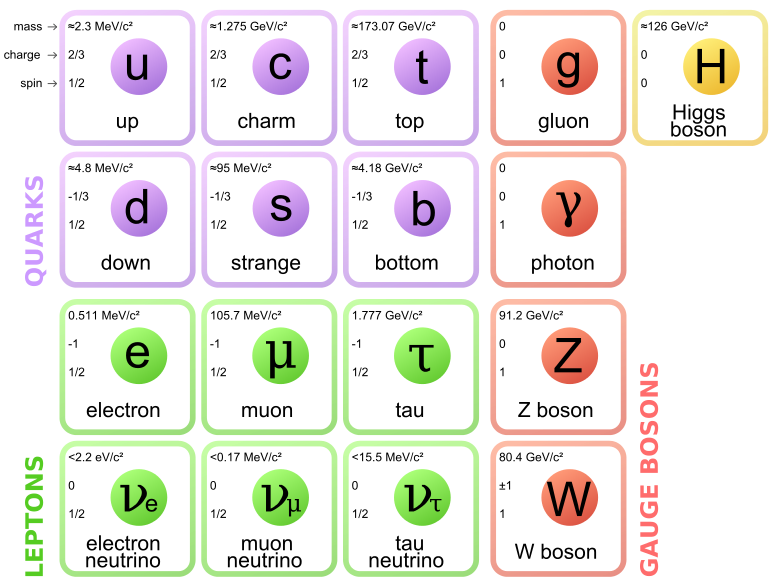
\includegraphics[width=0.75\textwidth]{./Chapters/theory/standard_model/images/particle_table.png}
	\caption{Table of particles in the Standard Model \cite{particle_table}}
	\label{fig: particle table}
\end{figure}
%%\subsection*{Interactions}

%\input{./Chapters/theory/standard_model/electromagnetism}
%\input{./Chapters/theory/standard_model/strong_interaction}
%\input{./Chapters/theory/standard_model/weak_interaction}
%\input{./Chapters/theory/standard_model/electroweak_interaction}
%\input{./Chapters/theory/standard_model/higgs_mechanism}
\subsection{Quantum Field Theory (QFT)}

Quantum field theory is built on concepts from Quantum Mechanics, Special Relativity and Classical Field Theory. Fundamental particles are described as excitations or quanta of the fields. For example, electrons are quanta of the electron field and similarly photons are quanta of the electromagnetic field i.e. interactions between electrons can be described as being a result of the interaction between the electron field and electromagnetic field. Mathematically these interactions can be described using the Lagrangian Formalism. 

\subsubsection{Lagrangian Formalism}
With Lagrangian mechanics the equations of motion for a given field is derived by minimising the action $\mathcal{S}$ given by,

\begin{equation}
	\mathcal{S} = \int\mathcal{L}(\phi, \partial_\mu \phi) \mathrm{d}^4x
\end{equation}

where $\mathcal{L}$ is the Lagrangian density, $\phi$ is the field and $\partial_\mu$ is the differential operator acting on the space and time coordinates of the field as seen in special relativity. By applying the condition of the Principle of Least Action, the equations of motion are given by the Euler-Lagrange equation,

\begin{equation}
	\partial_\mu(\frac{\partial\mathcal{L}}{\partial(\partial_\mu\phi_i)}) = \frac{\partial\mathcal{L}}{\partial\phi_i}
\end{equation}

\input{./Chapters/theory/standard_model/gauge_transformations.tex}
\input{./Chapters/theory/standard_model/coupling_constants.tex}
\input{./Chapters/theory/standard_model/qed.tex}
\subsection{Quantum Chromodynamics (QCD)}

% OVERVIEW
%
%   * a theory of the strong interaction (color force)
%   * It is the study of the SU(3) Yang�Mills theory of color-charged fermions (the quarks)  
%   * Described by the SU(3) group
%   * QCD is a gauge theory of the SU(3) gauge group obtained by taking the color charge to define a local symmetry. 


QCD is a physical theory that describes the interactions between particles with the property of colour via strong interactions. It is a gauge theory with a symmetry group of SU(3) (the group of unitary matrices with a determinant of one) and describes the interactions between quark and gluon fields. 

The strong force is responsible for the binding force which holds nucleons together to form the nucleus of an atom. This is due to the deeper fundamental interaction between the components of nucleons - quarks and gluons - collectively called partons. The gluons are the gauge bosons of the theory i.e. mediators of the strong force. It is a short range force having a significant effect only on scale of $\sim1$ fm (about the size of the charge radius of a proton) due to the nature of its coupling. The Lagrangian of QCD is,

\begin{equation}
	\mathcal{L} = \bar\psi_i i((\gamma^\mu D_\mu)_{ij} - m \delta_{ij})\psi_j - \frac{1}{4}G^a_{\mu\nu}G^{\mu\nu}_a
	\label{equation: qcd lagrangian}
\end{equation}

where $\bar\psi_i$ is the quark field and $G^a_{\mu\nu}$ is the gluon field strength tensor given by,

\begin{equation}
	G^a_{\mu\nu} = \partial_\mu A^a_\nu - \partial_\nu A^a_\mu + gf^{abc} A_\mu^b A_\nu^c
\end{equation}

where $A^a_\nu$ are the gluon fields and $f^{abc}$ are the fine structure constants of the SU(3) group.

%BOUND STATES
Quarks have been observed in two-quark bound states (mesons) and three-quark bound states (baryons); the six flavours of quarks give rise to many possible quark combinations, these combinations are commonly grouped into octets by the eightfold way, figure \ref{fig: eightfold way}.


%\subsection*{Parton Bound States}
%The three colours form a quark triplet, 

%\begin{equation}
%	c = \[
%	\left(
%	\begin{array}{c}
%		\psi_1 \\
%		\psi_2 \\
%		\psi_3   
%	\end{array}
%	\right)
%	\]
%\end{equation}

\begin{figure}[h]
	\begin{subfigure}[h]{0.49\textwidth}
		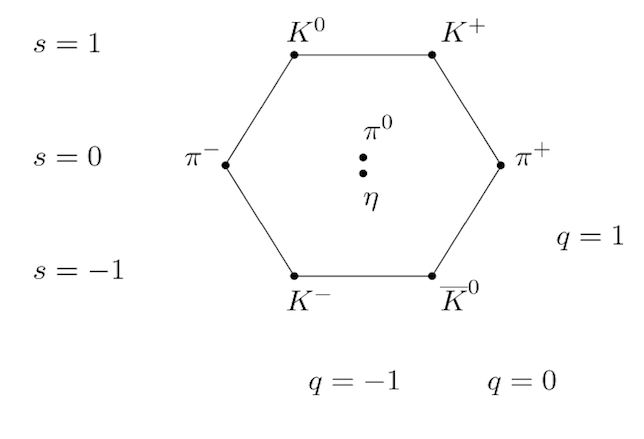
\includegraphics[width=\textwidth]{./Chapters/theory/standard_model/images/meson_octet.png}
		\caption{The meson octet (two quark bound states)}
		\label{fig: meson octet}
	\end{subfigure}
	\begin{subfigure}[h]{0.49\textwidth}
		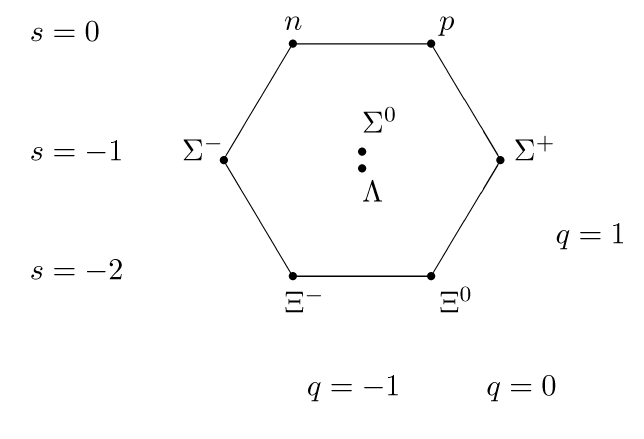
\includegraphics[width=\textwidth]{./Chapters/theory/standard_model/images/baryon_octet.png}
		\caption{Baryon octet (three quark bound states)}
		\label{fig: baryon decuplet}
	\end{subfigure}
	\caption{Eightfold method of organising quark bound states. Bound states on the same horizontal share the same strangeness and those on the same diagonals running top left to bottom right share the same charge}
	\label{fig: eightfold way}
\end{figure}

% COLOUR
The property of colour in QCD is analogous in many ways to the role of electric charge in QED. However instead of there being one type of charge in QCD there are three types, labelled red, green, blue and their corresponding anti-colours anti-red, anti-green and anti-blue. The names of the charge types are motivated by the behaviour of coloured light such that a bound state of a red, blue and green quarks gives a net colour charge of white or colourless; a combination of colour and anti-colour is also colourless.

% PARTONS
Each quark possesses one of the three types of colour charge; it can be either red, green or blue (similarly so for anti-quarks and the anti-colour charges). Gluons on the other hand possess a combination of colour and anti-colour charge (though these charges are not necessarily of the same colour). Since gluons are charged, QCD features some additional richness not seen in its QED counterpart. Gluons can couple with one other unlike photons which cannot, see figure \ref{fig: qcd field couplings}.

\begin{figure}[h]
	\centering
	\begin{subfigure}[h]{0.32\textwidth}
		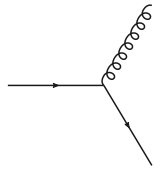
\includegraphics[width=0.8\textwidth]{./Chapters/theory/standard_model/images/quark_gluon.png}
		\caption{Quark-gluon vertex}
		\label{fig: quark-gluon vertex}
	\end{subfigure}
	\begin{subfigure}[h]{0.32\textwidth}
		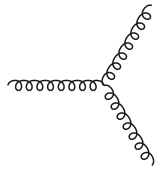
\includegraphics[width=0.8\textwidth]{./Chapters/theory/standard_model/images/gluon3.png}
		\caption{Three-gluon vertex}
		\label{fig: three-gluon vertex}
	\end{subfigure}
	\begin{subfigure}[h]{0.32\textwidth}
		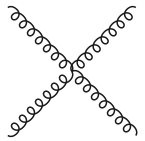
\includegraphics[width=0.8\textwidth]{./Chapters/theory/standard_model/images/gluon4.png}
		\caption{Four-gluon vertex}
		\label{fig: four-gluon vertex}
	\end{subfigure}
	\caption{QCD field couplings}
	\label{fig: qcd field couplings}
\end{figure}

\subsection*{Asymptotic freedom}
The coupling constant $\alpha_s$ of QCD describes the strength of the strong interaction. The $\beta$ function for the strong coupling constant is given by,

\begin{equation}
	\beta(\alpha_s) = - \left(11 - \frac{2n_f}{3}\right)\frac{\alpha_s^2}{2\pi}
\end{equation}
where,
\begin{equation}
	\alpha_s = \frac{g^2}{4\pi}
\end{equation}

and $n_f$ is the number of quark flavours in the theory. Since there are six quark flavours in the standard model the values of the $\beta$ function are negative i.e. the coupling constant of the strong force decreases with an increase in the energy transfer (or equivalently a decrease in the distance) of the process. The running coupling constant as a function of the energy transfer is given by,

\begin{equation}
	\alpha_s(|q^2|) = \frac{4\pi}{(11 - \frac{2n_f}{3})\mathrm{ln}(|q^2|/\Lambda^2)} \,\,\,\,\,\, (|q^2| >> \Lambda^2)
\end{equation}

where $|q^2|$ is the energy transfer of the process and $\Lambda$ is the QCD scale defined as the energy transfer at which the strong coupling constant $\alpha_s \sim 1$ and perturbative calculations with expansions of the coupling constant diverge.

This behaviour of the strong force coupling constant to become weaker at short range interactions is known as asymptotic freedom. Quarks and gluons which interact over short distances - such as at high energy collider experiments - interact very weakly and act as quasi-free particles. Since the coupling constant is small in this regime perturbative methods can also be used calculate properties of the theory.

\subsection*{Colour Confinement}
Colour confinement is an observed phenomenon in which partons are only observed in bound colour singlets states, i.e. no individual free quarks or gluons have been observed. As quarks are separated the coupling constant increases such that the energy needed to separate them increases indefinitely. At some energy threshold the system of separating quarks will have enough enough energy to spontaneously form quark anti-quark pairs - forming a bound state with the initial quarks. This process - called hadronisation - may occur multiple times resulting in a shower of particles called a jet. Since the strong coupling constant is inherently large in these processes perturbative methods are incompatible with describing this behaviour, instead our best understanding is achieved by phenomenological models (see section \ref{section: hadronisation}). 

%\input{./Chapters/theory/standard_model/qcd_factorisation_theorem}

% and lattice QCD which is based on the principle of quantising space and time into a lattice. 

%Colour confinement is deeply tied into understanding particle production in particle collision experiments. In the case of a scattering experiment of a composite object without components such as photon-electron scattering in an atom, the energy transfer may result in the electron being freed from the atom overcoming the electromagnetic attractive forces (the photoelectric effect). However in the case of coloured objects such as quarks this does not occur. In the theory of QCD quark-quark interactions from proton-proton collisions with large enough energies to separate the initial quarks in a proton by a threshold distance resulting in the spontaneous production of quark-antiquark pairs, each quark binding with either of the other quarks in the proton or with the separated quark such that only composite objects are present in the final state of the interaction.

%The phenomena of colour confinement and asymptotic freedom pose many challenges for physicists due primarily to the behaviour of the strong coupling constant. Unlike the coupling constants for the electromagnetic and weak interactions increases with distance between correspondingly charged particles. Perturbative calculations expanded about the strength of the coupling constant diverge meaning the calculations become invalid.

%When quarks in bound states such as mesons and baryons are separated from each other, the increasing strength of the strong interaction between them may result in the spontaneous creation of quark-antiquark pairs, these are generally referred to as showers or jets of hadrons. Since the strong coupling constant is large in these processes it is not possible to calculate the probability of these processes from the fundamental Lagrangians of the Standard Model. Instead separate hadronisation models such as the Lund String model discussed in section \ref{section: hadronisation} are used instead. Ideally jet behaviour would be described by the Lagrangians of the Standard Model, however a complete understanding of this behaviour still has its challenges - though much progress has been made by hadronisation models.


% SU(3)

% LAGRANGIAN 
%These interactions correspond to the three and four gluon vertex diagrams seen in the Feynman diagram representation and by the corresponding Lagrangian terms (see equation \ref{equation: qcd lagrangian} and figure \ref{fig: qcd field couplings}).


%\subsection{Electroweak Interaction}

\subsubsection{The Higg's Mechanism}
%\subsection{Beyond the Standard Model}
\section{QCD in Proton Collider Experiments}

The complexity of QCD shown in colour confinement and the running of the strong coupling constant present additional challenges in experimental physics. In order to describe the behaviour of QCD phenomena with perturbative methods the strong coupling constant must be small such that a perturbative expansion in powers of the coupling constant converge. This is true in the case short range interactions where asymptotic freedom is present though this is not the case for long range interactions at the scale of $\Lambda_{QCD}$.

Colour confinement tells us that coloured particles can only be observed in colour singlet states called hadrons. The size of hadrons ($\sim 1$ fm) corresponds to a energy scale of approximately $200$ MeV ($\approx \Lambda_{QCD}$), hence, the observable particles associated to QCD are coupled to long range physics - i.e. incompatible with a purely perturbative description. To describe such states a combination of perturbative and non-perturbative approaches must be used.

% FACTORISATION IS
\subsection{Factorisation}
Factorisation is the process of decoupling the hard and soft scale physics in QCD phenomena into products of hard and soft scale terms. By factorising the problem, the well understood perturbative methods can be used to calculate terms involving hard scale interactions - where $\alpha_s << 1$ - and non-perturbative methods are used to calculate the remaining contributions from soft scale physics. 

% FACTORISATION SCHEME
The hard process is described by a matrix element calculated using the perturbative Feynman approach from the QCD Lagrangian. The soft physics is characterised by a parton distribution function which describes the density and momentum of quarks within the proton. Cross sections are then calculated by convoluting the parton level cross section with the parton distribution function.

For the process, $ij \rightarrow k$ in a proton-proton interaction, the cross-section $\sigma_{ij\rightarrow k}$ is described by,

\begin{equation}
	\sigma_{ij\rightarrow k} = \int \mathrm{d}x_1 \int \mathrm{d}x_2 f_i^1(x_1)f_j^2(x_2) \hat{\sigma}_{ij \rightarrow k}
\end{equation}

where $\hat{\sigma}$ is the cross-section for hard partonic cross-sections and $f_i^1$ is the parton distribution function describing the probability of finding a parton of type $i$ in the beam proton $1$ with momentum fraction $x_1$; similarly $f_i^2$ describes the distribution of partons for beam proton 2.

%$x_1$ and $x_2$ are the longitudinal momentum fraction of the interacting partons from protons 1 and 2; 

%PARTON DISTRIBUTION FUNCTIONS 
Due to the non-perturbative nature of parton distributions, their determination is through fits to experimental data such as from deep inelastic scattering experiments. The parton distribution functions are universal in that the parton distribution function calculated from one experiment may be used as input for another. For experiments involving different energies the behaviour of the parton distribution functions at different energy scales is described by the DGLAP evolution equations \cite{Altarelli:1977zs}. 
% It is conventional to call the first term on the right of the above equation the leading twist contribution. The remainder is called the higher twist correction. It is formally of order 1/Q2 but not precisely known.

% LORENTZ EFFECTS
Protons accelerated to high energies are highly boosted in the laboratory rest frame, the proton is Lorentz contracted in the direction of the beamline and time dilated so that its constituent partons appear frozen, each carrying a longitudinal momentum fraction $x$ of the total proton longitudinal momentum. The boost also ensures partons are well modelled as being collinear to its parent proton, i.e. $0 < x < 1$. The beam crossing time is short enough such that an interactions between partons in opposing beams can be modelled as a one-to-one interaction; i.e. interactions in the final state do not interfere with the initial parton-parton interaction. In this environment the proton-proton beams are well modelled as sources of quasi-free quarks and the interactions in the system are well described by a factorisation scheme.

%\subsection{Hadronisation}
\label{section: hadronisation}


%High momentum transfer implies the interaction is over a short distance, therefore, interacting partons from each beam particle can be modelled as interacting with one parton from the opposing beam particle
%Interactions which occur in the final state after the hard scatter are assumed to occur on time scales too long to interfere with the hard scatter; that is the interactions of the partons among themselves, which occur at time-dilated time scales before or after the hard scattering do not interfere with the hard scatter
%Scattering becomes incoherent (no interference effects), work with probabilities rather than amplitudes
%Consider the probability of an interaction between two "frozen" states of the two colliding protons, the cross section is approximated by the Born cross section
%These effects are more prevalent at higher centre of masses
%
%proton beams are treated as collections of partons: quasi free quarks and gluons
%
%It is convenient to consider a frame in which the target nucleon has a very large momentum. In such a frame the momentum of the parton is almost collinear with the nucleon momentum, so that the target can be seen as a stream of partons, each carrying a fraction x of the longitudinal momentum
%
%The factorisation approach has had great success in demonstrating the predictive powers of QCD. 
%\subsection{Hadronisation}
\label{section: hadronisation}
%\subsection{The Underlying Event}
\label{section: underlying event}

The underlying event is any other activity in an event that accompanies a hard process, it contains contributions from the beam remnants - the left over proton fragments after the hard scatter - multiple parton interactions and initial and final state radiation. The hard scatter consists of the two outgoing jets, the initial state radiation leading to the hard process and the particles originating from the hard final state radiation.

The beam remnants are particles that evolves from the remainder constituents of the beam particle that do not take part in the hard process. These may be colour connected to the hard process due to colour confinement e.g. for a proton-proton interaction, a proton that initiates a hard process via a quark initiator will have remaining constituents that form a colour triplet. The colour connections are later resolved during the hadronisation process which ensures the final state of the interaction is composed of colour singlet hadrons. 

%Pythia: Highly developed multiple interaction model
%HERWIG: A MPI model is built into Herwig++ but a separate module (JIMMY) has to be interfaced to the Fortran version

%Lorentz contraction of highly boosted beam particles in result in disc like shapes in the laboratory rest frame. Interacting partons from the beam particles are extremely localised such that the parton shower and subsequent hadronisation are also. An overlap between the other partons in the beam particles giving rise to the potential of Multiple Parton Interactions (MPI) each with their own associated parton shower and hadronization. The additional interactions in multiple parton interactions are dominated by soft interactions though contributions exists from hard and semi-hard interactions. 

% and have been shown to have a significant effect on the particle multiplicity of the event.


% Beam remnant: Particles which do not take an "active" part in the initial-state radiation or hard-scattering process.
% 	Is colour connected to the primary 
% Multiple interactions: When more than one parton from each beam particle have "significant" interactions. in a fraction of events these additional scatterings maybe hard or semi-hard, but mostly they are soft in comparison to the hard process
% 	Important to model the impact parameter structure of hadron-hadron collisions
%	Impact parameter: Measure of how much overlap there is between hadrons
%		If it is small there is a high probability of multiple interactions
%		if it is small there is a high probability of a hard scatter
%		thus if it is small there is on average a higher amount of underlying event activity
%		if it is large there is a small probability of multiple interactions
% Primordial $k_\perp$: Transverse momentum of the shower initiating parton - takes into account the motion of quarks inside the original hadron.
% Underlying event: Arises from collisions between partons in the incoming hadrons that do not directly participate in the hard subprocess
% 	Everything except the hard radiation from the matrix element in the hard process for a single particle collision
% 	Minimum bias data - not identical but still related. Used to study correlations...

% MPI
%The most common hard subprocess at a high-energy hadron collider, such as the LHC, is elastic gluon-gluon scattering, $gg \rightarrow gg$ . The leading-order differential cross section for this subprocess diverges at zero momentum transfer, due to the exchange of a massless virtual gluon. This indicates that there are many interactions between beam particles though of a soft nature. 

%Multiple parton interactions is a term used to describe a proton-proton collision in which more than one parton from each of the protons are involved in an interaction. In general a proton-proton interaction is described by its primary interaction i.e. the parton interaction at the highest interaction scale, relative to this additional interactions are soft scale interactions due to an asymptotically decreasing cross-section with the interaction scale. However the probability of additional interactions that are hard or semi-hard is significant and has considerable effects on distributions such as the particle multiplicity.

% Why is it important
%A rather mundane reason for this is that if two pairs of partons collide in a single proton-proton collision, this can lead to some very peculiar-looking events. Two "standard" collisions can gang up and look very non-standard, possibly leading you to think you have found some physics beyond the Standard Model. (Probably supersymmetry.) So if you want to claim this, you need some understanding of the probability of multiparton interactions occurring in a single proton-proton collision.
%
%But on top of that, the issue of how a strongly interacting quantum field theory gives rise to the proton, an ultra-stable bound state with a lifetime longer than the age of the universe, present in the heart of every atom of matter, is an exciting open question. It's a problem being tackled from several experimental, theoretical and computational directions. I think understanding correlations between partons in high energy collisions will make an important contribution to this.
\section{Monte Carlo Generators}
\label{section: mc generators}

Monte Carlo (MC) generators are computational software used to simulate high energy processes. They use the principles of random sampling to emulate quantum mechanical phenomena together with the Standard Model and phenomenological models to describe particle interactions. %Since these processes are computed this gives physicists a full and exclusive modelling of high energy processes.

%Event generation is composed of two phases. The first is the generator stage which simulates the interaction between two initial particles (generally beam particles such as the proton-proton beams at the LHC) and the resulting particles from the parton interaction including their subsequent decays and the remnants (beam remnants in the case of LHC interactions). The second stage simulates the interactions between the particles produced in the initial stage and the components of the detector. This includes the simulation of particles which are produced from interactions with detector material as well as electromagnetic fields present in the detector. Furthermore the electronic signals from the detector components are also simulated. In the case of a perfect detector the result of the detector simulation would yield the particles produced in the generator stage, though in practise this is not the case.

MC generators are important for many aspects of high energy physics. They enable physicists to develop an understanding of how physics models translate to real world experiments bridging between the theoretical and experimental aspects of high energy physics. MC generators provide physicists insight into the frequency of specific types of events as well as the angular distribution of the resultant particles. This enables physicists to estimate the signal to background ratios of specific processes and provide insight into which regions of phase space provide the greatest level of sensitivity for a given process. Understanding the distribution of the resultant particles from a given type of interaction enables highly specialist detector design optimised for sensitivity to a given process.

MC generators are extremely sophisticated programs due to the complexity of high energy process. This process is simplified by factorising the process into several steps. First a hard process is simulated with associated initial state radiation followed by the hadronisation process and final state radiation as well as beam remnants. These components are discussed in the following sections and are visualised in figure \ref{fig: event schematic}.

\begin{figure}[h]
	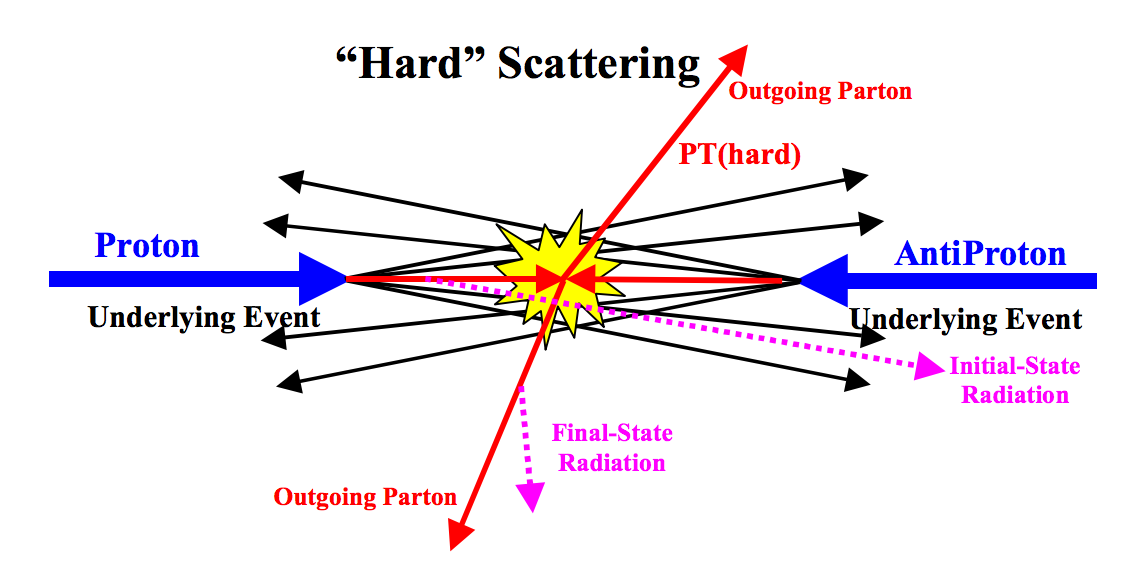
\includegraphics[width=\textwidth]{/Users/admin/projects/phd/thesis/latex/Chapters/theory/mc_generators/images/event_schematic.png}
	\caption{An event schematic demonstrating the aspects of the interaction \cite{Field:2002vt}}
	\label{fig: event schematic}
\end{figure}

%MC generators are extremely sophisticated programs though complexity of high energy processes rivals this. In order to make the process of event generation simpler the process is decomposed into components simplifying the problem via the principle of factorisation. Several of these components are discussed in the following sections.

%\subsection{Physics Model}
\subsection{The Hard Process}

The hard process is described by the parton interaction with the highest momentum transfer, it characterises the properties of the event such as the distribution of particles in the system and their energies. In general, experimentalists are interested in events involving a particular hard process, such as the production of exotic flavoured states, e.g.

\begin{equation}
	\mathrm{gg} \rightarrow \mathrm{c\bar{c}}
\end{equation}

describing the process of gluon fusion forming a charm quark-antiquark pair.

The hard process is the first stage of a MC event simulation, next a backwards time evolution is performed on the initiator partons to describe the system before the interaction. In the proton-proton event case this corresponds to the state of the incoming proton pairs. Similarly a forward time evolution is applied to the outgoing partons of the interaction to describe the final state of the system.

The forward evolution is divided into two phases, the first stage describes the radiation of quarks and gluons from the outgoing partons as a series of parton branchings evolving the system from a state with a low number of high momentum partons to a state with a high number of low momentum partons (parton shower \ref{section: parton shower}). This process describes the branchings using perturbative calculations down to a momentum threshold where perturbative methods are no longer applicable. Similarly an upper momentum threshold exists; partons with a momentum greater than this threshold are assigned to the hard process of the event.

The second phase takes the output of the parton shower and evolves it into a system of colourless hadrons using non-perturbative phenomenological models via the process of hadronisation (section \ref{section: hadronisation}). 

%
%\begin{equation*}
%	Q >> \Lambda
%\end{equation*}
%
%where $Q$ is the momentum transfer in the process and $\Lambda$ is the QCD scale ($217^{+25}_{-23}$ MeV), the strong coupling constant for these momentums is small allowing the cross-section for these processes to be calculated perturbatively.

\subsection{Initial and Final State Radiation}
\label{section: parton shower}

Initial state radiation is composed of partons that are emitted from the  beam particles. In the case of proton beams this is modelled as virtual particles being exchanged between the quark constituents; these virtual particles primarily consist of gluons which may further radiate pairs of gluons creating a complicated state of the proton. Similarly final state radiation consists of a myriad of partons but in this case the partons originate from the out-going partons of the hard scatter and initial state radiation.

The probability for branching to occur is generally calculated in one of two ways, either with a matrix element calculated from Feynman diagrams or with the parton shower model. The parton shower model is a simplified version of the matrix element approach with approximations including a simplification of kinematics, interference and helicity structure. Though the matrix element calculations are truer to the theory of QCD, in practice the matrix elements are more difficult to calculate - especially at higher orders. The two approaches are complementary to one another and which approach is used is based on the particular situation. In general the parton shower is chosen as the first place to start due to its flexibility and simplicity whilst for precision measurements the matrix element approach is favoured.

\subsubsection*{Parton Showers}
The parton shower is made up of branchings of the form $a \rightarrow bc$, e.g for quark-gluon radiation this is, 

\begin{equation*}
	q \rightarrow qg
\end{equation*}

Each of the partons in a shower are characterised by its virtuality scale $Q^2$ which gives an approximate sense of its time ordering in the shower, classically it is defined as the invariant mass of the parton; under this definition a system with a low number of high mass partons evolving into a high number of low mass partons will decrease in the virtuality scale as more and more branchings occur. The $Q^2$ variable may also be described by other variables such as its transverse momentum which similarly decreases with the number of branchings. A maximum virtuality scale $Q_{\mathrm{max}}$ distinguishes partons that are involved in the hard process from those in the parton shower, also a minimum virtuality scale $Q_0$ sets the scale at which non-perturbative effects become significant.

Partons with $m^2 < 0$  and $m^2 \ge 0$ are described as space- and time-like respectively. 

\subsubsection*{Initial State Radiation (ISR)}
For initial state radiation the virtuality scale is typically associated to the mass of the parton given by the equation,

\begin{equation}
	Q^2 = -m^2 = -(E^2 - p^2)
\end{equation}

The branching evolution of initial state radiation is described by increasing values of the virtuality scale $Q^2$, this corresponds to a high energy parton from a beam particle emitting partons with increasing virtuality and momentum i.e. the branching partons become more space-like. The branching continues until there are enough partons with $Q^2 \ge Q^2_{\mathrm{max}}$ to initiate the hard process; thus limiting the virtuality of the system, for example, the virtuality of the partons in the process $q\bar{q} \rightarrow Z^0$ have a virtuality cut off of the order of the $2m_{Z^0}$.

In order to generate an event with a particular hard process the shower algorithm first sets the longitudinal momentums $x_1$ and $x_2$ of the incoming partons to that required by the hard process using the parton distribution function. A backward time evolution is then applied to the partons, gaining energy with each emission and decreasing in virtuality until it is compatible with a shower initiating parton in the proton.

\subsubsection*{Final State Radiation (FSR)}
For final state radiation the initiating shower parton originates from the outgoing partons of the hard interaction via time-like partons. The virtuality scale for partons is typically defined by either its invariant mass or transverse momentum.

\begin{equation}
	Q^2 = m^2
\end{equation}
or
\begin{equation}
	Q^2 = p_\perp^2
\end{equation}

note the change in sign in the mass ordering relative to the ISR. The final state evolves with a decreasing virtuality scale - becoming more time-like. Starting from an outgoing parton from the hard process the branching results in partons with lower mass or transverse momentum depending on the choice of ordering parameter. The minimum virtuality of a parton is set by $Q_0$, partons which cannot branch further due to this cutoff are then used as input for the hadronisation process.

%There are several options for the evolution parameter for final final state radiation. Most common are the invariant mass $m$ and the transverse momentum of the parton $p_\perp$. In contrast to initial state radiation the evolution parameter generally decreases with more branchings, 

%Final state radiation consists of partons radiated from the outgoing partons of the hard process. The cascade of partons are modelled by the DGLAP equations and works downwards to lower momentum scales to a point where perturbation theory breaks down. At this point the partons are evolved to colourless hadrons via the process of hadronization.
\subsection{Hadronisation}
\label{section: hadronisation}
\subsection{The Underlying Event}
\label{section: underlying event}

The underlying event is any other activity in an event that accompanies a hard process, it contains contributions from the beam remnants - the left over proton fragments after the hard scatter - multiple parton interactions and initial and final state radiation. The hard scatter consists of the two outgoing jets, the initial state radiation leading to the hard process and the particles originating from the hard final state radiation.

The beam remnants are particles that evolves from the remainder constituents of the beam particle that do not take part in the hard process. These may be colour connected to the hard process due to colour confinement e.g. for a proton-proton interaction, a proton that initiates a hard process via a quark initiator will have remaining constituents that form a colour triplet. The colour connections are later resolved during the hadronisation process which ensures the final state of the interaction is composed of colour singlet hadrons. 

%Pythia: Highly developed multiple interaction model
%HERWIG: A MPI model is built into Herwig++ but a separate module (JIMMY) has to be interfaced to the Fortran version

%Lorentz contraction of highly boosted beam particles in result in disc like shapes in the laboratory rest frame. Interacting partons from the beam particles are extremely localised such that the parton shower and subsequent hadronisation are also. An overlap between the other partons in the beam particles giving rise to the potential of Multiple Parton Interactions (MPI) each with their own associated parton shower and hadronization. The additional interactions in multiple parton interactions are dominated by soft interactions though contributions exists from hard and semi-hard interactions. 

% and have been shown to have a significant effect on the particle multiplicity of the event.


% Beam remnant: Particles which do not take an "active" part in the initial-state radiation or hard-scattering process.
% 	Is colour connected to the primary 
% Multiple interactions: When more than one parton from each beam particle have "significant" interactions. in a fraction of events these additional scatterings maybe hard or semi-hard, but mostly they are soft in comparison to the hard process
% 	Important to model the impact parameter structure of hadron-hadron collisions
%	Impact parameter: Measure of how much overlap there is between hadrons
%		If it is small there is a high probability of multiple interactions
%		if it is small there is a high probability of a hard scatter
%		thus if it is small there is on average a higher amount of underlying event activity
%		if it is large there is a small probability of multiple interactions
% Primordial $k_\perp$: Transverse momentum of the shower initiating parton - takes into account the motion of quarks inside the original hadron.
% Underlying event: Arises from collisions between partons in the incoming hadrons that do not directly participate in the hard subprocess
% 	Everything except the hard radiation from the matrix element in the hard process for a single particle collision
% 	Minimum bias data - not identical but still related. Used to study correlations...

% MPI
%The most common hard subprocess at a high-energy hadron collider, such as the LHC, is elastic gluon-gluon scattering, $gg \rightarrow gg$ . The leading-order differential cross section for this subprocess diverges at zero momentum transfer, due to the exchange of a massless virtual gluon. This indicates that there are many interactions between beam particles though of a soft nature. 

%Multiple parton interactions is a term used to describe a proton-proton collision in which more than one parton from each of the protons are involved in an interaction. In general a proton-proton interaction is described by its primary interaction i.e. the parton interaction at the highest interaction scale, relative to this additional interactions are soft scale interactions due to an asymptotically decreasing cross-section with the interaction scale. However the probability of additional interactions that are hard or semi-hard is significant and has considerable effects on distributions such as the particle multiplicity.

% Why is it important
%A rather mundane reason for this is that if two pairs of partons collide in a single proton-proton collision, this can lead to some very peculiar-looking events. Two "standard" collisions can gang up and look very non-standard, possibly leading you to think you have found some physics beyond the Standard Model. (Probably supersymmetry.) So if you want to claim this, you need some understanding of the probability of multiparton interactions occurring in a single proton-proton collision.
%
%But on top of that, the issue of how a strongly interacting quantum field theory gives rise to the proton, an ultra-stable bound state with a lifetime longer than the age of the universe, present in the heart of every atom of matter, is an exciting open question. It's a problem being tackled from several experimental, theoretical and computational directions. I think understanding correlations between partons in high energy collisions will make an important contribution to this.
\subsection{Multiple Parton Interactions (MPIs)}
%Multiple parton interactions is a term used to describe a proton-proton collision in which more than one parton from each of the protons are involved in an interaction. In general a proton-proton interaction is described by its primary interaction i.e. the parton interaction at the highest interaction scale, relative to this additional interactions are soft scale interactions due to an asymptotically decreasing cross-section with the interaction scale. Though the probability of hard or semi-hard additional interactions are smaller than for soft interactions at higher energies this increases due to the ability of partons to resolve partons in the proton with lower longitudinal momentum fraction $x$.

Multiple parton interactions is a term used to describe a proton-proton collision in which there is more than one hard scatter between the constituent partons. Observations of MPI effects can be seen in data from hadron collisions at the Intersecting Storage Rings (ISR) at CERN \cite{Akesson:1986iv} and the Fermilab Tevatron collider \cite{Abe:1997bp} \cite{Drees:1996rw} \cite{Abazov:2009gc}. Soft MPI effects have been observed in proton-proton collisions at Collider Detector Fermilab (CDF) \cite{Acosta:2004wqa} \cite{Aaltonen:2010rm} and CMS \cite{Khachatryan:2010pv}.

%The evidence for MPI comes from high pT events observed in hadron collisions at the ISR at CERN [1] and later
%at the Fermilab Tevatron collider[2, 3, 4]. At lower pT, underlying event (UE) observables have been measured in pp
%collisions in dijet and Drell-Yan events at CDF in Run I [5] and Run II [6] at centre-of-mass energies of p
%s = 1:8 TeV
%and 1:96 TeV respectively, and in pp collisions at p
%s = 900 GeV in a detector-specic study by CMS [7].
%At small transverse momentum MPI have been shown to be necessary for the successful description of th

It is important to understand MPI for several reasons. In the case of rare and exotic physics, two simultaneous non-exotic hard interactions may lead to non-standard looking events, it follows that in order to identify rare interactions and claim a discovery, one must have some understanding of the effects from MPI. Furthermore understanding MPI gives greater insight into the physics of the proton; one of the most stable bound states and fundamental constituents of ordinary matter.

MPI models are generally dependent on modelling the impact parameter between incident protons - the minimum radial distance between their centroid trajectories. This gives the amount of overlap between the effective cross-sectional area of the protons, the smaller the impact parameter i.e. the greater the overlap, the greater the probability of interaction and thus multiple interactions. 

% Sources
% - http://arxiv.org/abs/1111.0469, Multi-Parton Interactions at the LHC, Nov 2011
\subsection{Pythia}
\label{section: pythia}

% Sources
%   Pythia manual: 
%      http://home.thep.lu.se/~torbjorn/pythia/lutp0613man2.pdf
%      \cite{Sjostrand:2006za}
%
%   MC Generators for LHC: http://pi.physik.uni-bonn.de/pi_plone/files/TPSeminar/WS200910/JudithKatzy19Nov09.pdf
%
%   Monte Carlo Event Generators (PDG): 
%      http://pdg.lbl.gov/2013/reviews/rpp2012-rev-mc-event-gen.pdf
%      \cite{Nason:2013pdg}
%
%   Producing Hard Processes Regarding the Complete Event: The EPOS Event Generator: http://arxiv.org/abs/1006.2967
%
%   Les Houches Guidebook to Monte Carlo Generators for Hadron Collider Physics
%      http://arxiv.org/abs/hep-ph/0403045
%      \cite{Dobbs:2004qw}
%
%   Event Generators for LHC
%      http://cds.cern.ch/record/215298/files/CERN-90-10-V-2.pdf
%      Page 130
%      PDF page 72

\subsection*{Pythia}
Overview
\begin{itemize}
   \item A multi-purpose ``complete'' event generator.
   \item Commonly used in the field of high energy physics.
   \item Emphasis on simulating collisions between elementary particles, e.g. $\mathrm{e}^+\mathrm{e}^-$ and $\mathrm{pp}$ interactions.
   \item Uses the Lund model for hadronisation.
   \item JETSET is merged into PYTHIA.
\end{itemize}

JETSET
\begin{itemize}
  \item Developed by the Lund group in the 70's
  \item Aim: Understand hadronisation process.
  \item Focused on e+e- annihilation interactions
  \item By the mid 80's the matrix element method had reached its limit
  \item Parton shower model was developed
  \item The success of the parton shower lead attempts to use the model in other interactions, e.g. hadron interactions scattering in PYTHIA.
  \item In 1996 PYTHIA and JETSET are merged in PYTHIA 6.1.
\end{itemize}

Factorisation
\begin{itemize}
  \item Interactions are complicated, i.e. calculating the cross-sections using pertubative methods are difficult to carry out and interpret.
  \item Interactions can be simplified by using some assumprtions to break the interaction into phases (factorisation).
  \item The output from one phase serves as input for the next, analagous to a pipeline
  \item A phase is dependent only on it input, i.e. the output from previous phase
  \item e.g. Hadronic events at LEP 
  \begin{itemize}
    \item The main (hard) interaction is described by $\mathrm{e}^+\mathrm{e}^- \rightarrow \mathrm{Z}^0 \rightarrow \mathrm{q}\mathrm{\bar{q}}$
    \item Bremsstrahlung-type modifications i.e. the emission of additional final-state particles by branchings such as $\mathrm{e} \rightarrow \mathrm{e}\mathrm{\gamma}$ and $\mathrm{q} \rightarrow \mathrm{qg}$
    \item Higher order corrections - loops and soft bremsstrahlung
    \item Hadronisation. Not well understood from first principles due to confinement. Its modelling may have a significant effect on the event depending on what aspect of the event is being analysed. e.g. the charged particle multiplicity may vary significantly though the overall energy flow is mainly determined by perturbative processes.
  \end{itemize}
\end{itemize}

Lund Model / String fragmentation
\begin{itemize}
\item Long-range confinement forces are allowed to distribute the energies and flavours of a parton configuration among a collection of primary hadrons.
\item Predictions were confirmed by e+e- annihilation data at ~30GeV, whence gained widespread acceptance.
\item Currently the most complex and widely used fragmentation model.
\end{itemize}

Fragmentation vs Hadronisation
\begin{itemize}
  \item Hadronisation is the process of transforming colourless hadrons from coloured partons, i.e. quarks and gluons
  \item Hadronisation is sub-divided into fragmentation and decay
  \item Fragmentation is the break up of high mass coloured states into a system of colourless hadrons, e.g. jet -> hadron + remainder jet.
\end{itemize}

\subsection*{Pythia 6}

\subsection*{Pythia 8}

\subsection*{Pythia LHCb}

\subsection*{EPOS}

%\subsection{Generator Comparison}
\label{section: generator comparison}

% Sources
%   Pythia manual: 
%      http://home.thep.lu.se/~torbjorn/pythia/lutp0613man2.pdf
%      \cite{Sjostrand:2006za}
%
%   MC Generators for LHC: http://pi.physik.uni-bonn.de/pi_plone/files/TPSeminar/WS200910/JudithKatzy19Nov09.pdf
%
%   Monte Carlo Event Generators (PDG): 
%      http://pdg.lbl.gov/2013/reviews/rpp2012-rev-mc-event-gen.pdf
%      \cite{Nason:2013pdg}
%
%   Producing Hard Processes Regarding the Complete Event: The EPOS Event Generator: http://arxiv.org/abs/1006.2967
%
%   Les Houches Guidebook to Monte Carlo Generators for Hadron Collider Physics
%      http://arxiv.org/abs/hep-ph/0403045
%      \cite{Dobbs:2004qw}
%
%   Event Generators for LHC
%      http://cds.cern.ch/record/215298/files/CERN-90-10-V-2.pdf
%      Page 130
%      PDF page 72

\subsection*{Pythia}
Overview
\begin{itemize}
   \item A multi-purpose ``complete'' event generator.
   \item Commonly used in the field of high energy physics.
   \item Emphasis on simulating collisions between elementary particles, e.g. $\mathrm{e}^+\mathrm{e}^-$ and $\mathrm{pp}$ interactions.
   \item Uses the Lund model for hadronisation.
   \item JETSET is merged into PYTHIA.
\end{itemize}

JETSET
\begin{itemize}
  \item Developed by the Lund group in the 70's
  \item Aim: Understand hadronisation process.
  \item Focused on e+e- annihilation interactions
  \item By the mid 80's the matrix element method had reached its limit
  \item Parton shower model was developed
  \item The success of the parton shower lead attempts to use the model in other interactions, e.g. hadron interactions scattering in PYTHIA.
  \item In 1996 PYTHIA and JETSET are merged in PYTHIA 6.1.
\end{itemize}

Factorisation
\begin{itemize}
  \item Interactions are complicated, i.e. calculating the cross-sections using pertubative methods are difficult to carry out and interpret.
  \item Interactions can be simplified by using some assumprtions to break the interaction into phases (factorisation).
  \item The output from one phase serves as input for the next, analagous to a pipeline
  \item A phase is dependent only on it input, i.e. the output from previous phase
  \item e.g. Hadronic events at LEP 
  \begin{itemize}
    \item The main (hard) interaction is described by $\mathrm{e}^+\mathrm{e}^- \rightarrow \mathrm{Z}^0 \rightarrow \mathrm{q}\mathrm{\bar{q}}$
    \item Bremsstrahlung-type modifications i.e. the emission of additional final-state particles by branchings such as $\mathrm{e} \rightarrow \mathrm{e}\mathrm{\gamma}$ and $\mathrm{q} \rightarrow \mathrm{qg}$
    \item Higher order corrections - loops and soft bremsstrahlung
    \item Hadronisation. Not well understood from first principles due to confinement. Its modelling may have a significant effect on the event depending on what aspect of the event is being analysed. e.g. the charged particle multiplicity may vary significantly though the overall energy flow is mainly determined by perturbative processes.
  \end{itemize}
\end{itemize}

Lund Model / String fragmentation
\begin{itemize}
\item Long-range confinement forces are allowed to distribute the energies and flavours of a parton configuration among a collection of primary hadrons.
\item Predictions were confirmed by e+e- annihilation data at ~30GeV, whence gained widespread acceptance.
\item Currently the most complex and widely used fragmentation model.
\end{itemize}

Fragmentation vs Hadronisation
\begin{itemize}
  \item Hadronisation is the process of transforming colourless hadrons from coloured partons, i.e. quarks and gluons
  \item Hadronisation is sub-divided into fragmentation and decay
  \item Fragmentation is the break up of high mass coloured states into a system of colourless hadrons, e.g. jet -> hadron + remainder jet.
\end{itemize}

\subsection*{Pythia 6}

\subsection*{Pythia 8}

\subsection*{Pythia LHCb}

\subsection*{EPOS}


	
%	\subsection{Parton distributions}
%	\subsection{Hard Processes}
%	\subsection{Initial and final state radiation}
%		Radiation of gluons and photons from the incoming and outgoing patrons form the initial and final state radiation of the process which may result in the requirement of  corrections for the process, these effects become more significant the greater the energy in the event. \\
%		correction methods
%		\begin{itemize}
%			\item Matrix element: Feynman diagrams are calculated, order by order.
%			\begin{itemize}
%				\item analytical method
%				\item The "correct" method
%				\item difficult in practise
%				\begin{itemize}
%					\item Corrections become increasingly difficult for higher and higher orders, particularly loop diagrams
%				\end{itemize}
%			\end{itemize}
%			\item Parton shower
%			\begin{itemize}
%				\item parton shower is an initial final state radiation estimation technique
%				\item combination of two (or more) parton branchings
%				\item requires matrix element approximated through simplification of the kinematics
%			\end{itemize}
%		\end{itemize}
%	\begin{itemize}
%		\item both methods are complimentary, the better method depends on the situation
%		\item If an estimation of the radiation is sufficient then the parton shower model is used
%		\item High precision measurements such as of $\alpha_s$ use the matrix element method
%	\end{itemize}
%	\subsubsection{Parton showers}
%	\begin{itemize}
%		\item Radiation is categorised into two categories, initial and final state radiation
%		\begin{itemize}
%			\item initial: radiation from incoming partons
%			\item final: radiation from the hard scatter
%		\end{itemize}
%		\item Each parton is characterised with a virtuality scale, $Q^2$
%		\begin{itemize}
%			\item gives an approximate sense of time ordering to the cascade
%			\item has alternative definitions (2 in Pythia)
%			\item for initial state radiation the $Q^2$ value gradually increases as the hard interaction is approached
%			\item for final state radiation the $Q^2$ gradually decreases
%			\item shower evolution cut off at $Q_0$ (1 GeV for QCD branching)
%			\item above $Q_{max}$ the showers are matched to the hard scatter
%			\item for final state radiation the strategy is to evolve the original parton downwards in $Q^2$ until a branching occurs
%			\begin{itemize}
%				\item the $Q^2$ value of the parton determines its mass or $p_T$ (depending on the definition of $Q^2$
%				\item the daughters of the branched quark then take on the value of $Q^2$ of the parent and the process is iterated until the cut off $Q_0$ is reached
%			\end{itemize}
%			\item for initial state radiation the method is to apply a backwards evolution starting with the hard scatter of an evolved parton distribution
%		\end{itemize}
%	\end{itemize}
%	\subsection{Beam remnants}
%		\begin{itemize}
%			\item Prevalent in proton-proton collisions but can also occur for electron-positron colliders ($\gamma \gamma \rightarrow q \bar{q}$)
%			\item Partons from the beam remnants and hard scatter are colour connected
%			\item Primordial momentum $k_T$ is the transverse momentum of the shower initiator, reflecting the motion of the quarks in the proton
%			\item $k_T$ determined from a "suitable" distribution
%		\end{itemize}
%	\subsection{Multiple parton interactions (MPI)}
%		\begin{itemize}
%			\item For $e^+e^-$ interactions it is reasonable to assume that there is one hard scatter in the event
%			\item Not so for proton-proton interactions
%			\item One parton may scatter several times with multiple partons in the other beam
%			\item several partons from each of the beams may scatter
%			\item Several different options for modelling MPI in Pythia
%		\end{itemize}
%	\subsection{Hadronization models}
%		\begin{itemize}
%			\item QCD perturbation theory is valid at short distance (high momentum transfer) interactions
%			\item At long distances the strong force coupling is large and the perturbation sequence does not converge
%			\item Colour confinement requires that particles in the final state are colourless
%			\item Hadronisation: The combination of partons to produce a set of colourless hadrons	(also referred to as fragmentation)
%			\item A number of schools of phenomenological models have been developed to describe this process
%			\begin{itemize}
%				\item String fragmentation
%				\item Independent fragmentation
%				\item Cluster fragmentation
%			\end{itemize}
%			\item A good model should have,
%			\begin{itemize}
%				\item internal consistency
%				\item describe existing data well
%				\item high predictive power
%			\end{itemize}
%		\end{itemize}
%		\subsubsection{String fragmentation}
%			\begin{itemize}
%				\item default for Pythia
%				\item Lund model
%				\item branching parameters
%				\begin{itemize}
%					\item jet to hadron + remainder jet
%					\item string to hadron + remainder string
%					\item at each branching consider
%					\begin{itemize}
%						\item flavour production
%						\item distribution of energy and momentum
%					\end{itemize}
%				\end{itemize}
%			\end{itemize}
%			\paragraph{Lund model}
%				\begin{itemize}
%					\item Uses the idea of quantum mechanical tunnelling
%					\item Leads to flavour independent Gaussian spectrum for the $p_T$ of the $q \bar{q}$ pairs
%					\item Leads to suppression of heavy flavour quark production
%					\item Meson spin states are determined from the ratio of possible spin states multiplied by a wave function normalisation factor
%					\item Baryon production
%					\begin{itemize}
%						\item diquarks are treated as effectively as a single quark
%						\item popcorn model: quark-antiquark are produced one after the other
%					\end{itemize}
%					\item 
%				\end{itemize}
%				
%			\paragraph{Simple case scenario}
%				\begin{itemize}
%					\item Simplest scenario $e^+e^- \rightarrow q \bar{q}$, two jet event
%					\item lattice QCD studies suggest linear confinement, energy stored in the colour field increases linearly with separation (neglecting Coulomb interaction)
%					\item Separation of quarks creates a colour flux tube stretched between them
%					\item Mathematical Lorentz invariant description of this is of a massless relativistic string
%					\item As the energy in the string increases the string may break and produce a new $q \bar{q}$ pair
%				\end{itemize}

\section{Minimum bias data}

To minimise the bias of data from inelastic collisions collected from collider experiments, experimentalists use a trigger with a minimal set of criteria - generally called the minimum bias trigger. This trigger will typical involve requirements such as a minimum number of hits in an event or an event with at least one reconstructed track. Biases are still present due to collisions that are not detectable such as collisions that result in  particles with trajectories collinear to the initial trajectory of the beam particles; these particles continue along the beam pipe leaving no sign in the sensitive components of the detector. 

Collisions at the LHC can be classified into elastic (in which no additional particles are produced and inelastic) and inelastic collisions,
\begin{equation}
	\sigma_{tot} = \sigma_{elastic} + \sigma_{inelastic}
\end{equation}
which can be further classified into diffractive and non-diffractive collisions,
\begin{equation}
	\sigma_{inelastic} = \sigma_{non-diffractive} + \sigma_{single-diffraction} + \sigma_{double-diffraction}
\end{equation}
Diffractive collisions involve collisions that do not transfer colour between the beam particles and are characterised by events with large rapidity gaps with no hadronic activity. They can involve the break up of one of the incoming protons (single diffraction) or both (double diffraction, see figure \ref{fig: diffractive processes}). The events typically selected by a minimum bias trigger are made up of non-diffractive inelastic events with a small contributions from diffractive collisions.

\begin{figure}[h]
	\centering
	\begin{subfigure}[h]{0.32\textwidth}
		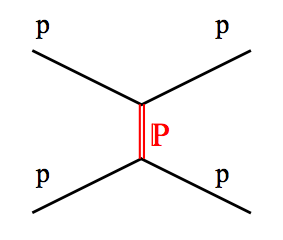
\includegraphics[width=\textwidth]{./Chapters/theory/minimum_bias/images/elastic_scattering.png}
		\caption{Elastic scattering, $p + p \rightarrow p + p$}
		\label{fig: proton-proton interactions - elastic scattering}
	\end{subfigure}
	\begin{subfigure}[h]{0.32\textwidth}
		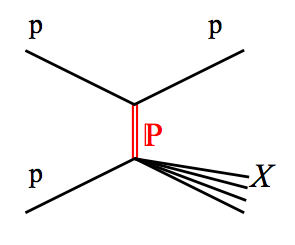
\includegraphics[width=\textwidth]{./Chapters/theory/minimum_bias/images/single_diffractive.png}
		\caption{Single diffractive scattering, $p + p \rightarrow p + X$}
		\label{fig: proton-proton interactions - single diffractive scattering}
	\end{subfigure}
	\begin{subfigure}[h]{0.32\textwidth}
		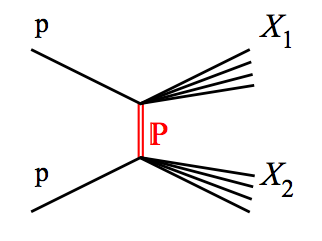
\includegraphics[width=\textwidth]{./Chapters/theory/minimum_bias/images/double_diffractive.png}
		\caption{Double diffractive scattering, $p + p \rightarrow X + X'$}
		\label{fig: proton-proton interactions - double diffractive scattering}
	\end{subfigure}
	\caption{Examples of elastic and inelastic proton-proton interactions via the exchange of a pomeron \cite{Kwiecinski:314736}.}
	\label{fig: elastic and inelastic proton-proton scattering}
\end{figure}

Minimum bias data is dominated by soft QCD physics characterised by low $p_T$ particles and long interaction distances. This property of minimum bias data makes it the ideal region in which to validate, tune and develop phenomenological models e.g. particle production and the structure of the proton. Furthermore minimum bias data is a good approximation of the underlying event (see section \ref{section: underlying event}) which accompanies a hard scale scatter; a good understanding of this translates to a good understanding of the associated hard energy scale physics such as the rare B decays integral to understanding matter and anti-matter physics.

 % Background Theory 
%	% Chapter 1

\chapter{The LHCb detector} % Write in your own chapter title\label{The LHCb detector}
\lhead{\emph{The LHCb detector}} % Write in your own chapter title to set the page header

\section{The Large Hadron Collider (LHC)}

The Large Hadron Collider (LHC) is located at the European Organisation for Nuclear Research (CERN) near Geneva in Switzerland. On the 23rd November 2009 the collider began producing collisions at a centre of mass energy of 900\gev. Over the course of its operation the energy of the collisions has increased, for proton-proton collisions the centre of mass energy was increased first to 7\TeV (28 February 2010) and then 8\TeV (5 April 2012) with a peak luminosity of the order $10^{34}\cm^{-2}\sec^{-1}$, making the LHC world's highest energy and luminosity particle accelerator. 

%As well as protons the LHC collides protons with heavy lead ions with dedicated runs in 2010 and 2011.

In the future the LHC intends to continue to push the energy and luminosity boundaries to reach unprecedented levels of high energy interactions and data collection. The goal being to produce collisions with a centre of mass energy of 14 TeV or greater. In addition to this, the sub-detector components will be upgraded to improve in areas such as detector readout rate and the resolution of kinematic quantities. Together with the increase in beam energy and luminosity this will give scientists at the LHC the ability to challenge the Standard Model at a level of greater detail than ever seen before.

Stationed at locations around the LHC are several detectors. The two counter-directional beams of proton bunches are focused at these positions such that a large number of collisions occur at the position of the detectors. The six main detectors, ALICE\cite{Aamodt:1129812}, ATLAS\cite{Aad:1129811}, CMS\cite{Chatrchyan:1129810}, LHCb\cite{Alves:1129809}, TOTEM\cite{Anelli:1129807} and LHCf\cite{Adriani:1129808} function as complementary experiments. A full discussion with regards to each detector at the LHC is beyond the scope of this thesis, therefore this thesis focuses on the most significant detector related to the research discussed, the LHCb detector.

% B production
% "LHC will be by far the most copious source of B mesons, due to the high $b\bar{b}$ cross section and high luminosity"
% "The LHCb experiment plans to operate with an average luminosity of $2 \times 10^{32}
% $10^{12} b\bar{b}$ pairs produced a year
% $b\bar{b}$ pairs are predominantly produced in the same forward cone. 
% Trigger selects B events based on particles with large transverse momentum and displaced decay vertices
% decay vertex resolution && particle Id, vertex resolution studying rapidly oscillating $B_s$ mesons 
% pion - kaon separation - Bd -> pi pi heavily contaminated by Bd -> Kpi, Bs -> Kpi and Bs->KK. => systematic errors in the measured CP asymmetry in Bd -> pipi decays.
% pion - kaon separation - Bs -> DsK, backgrounds: Bs -> Dspi (no CP violation is expected in Bs ->Dspi)
% < luminosity => < Detector occupancy && < radiation damage && < pile-up
\section{LHCb Overview}

The main aim of the LHCb experiment is to study CP violation processes and other rare phenomena particularly those involving the decay of  B and D mesons. Designed to build upon the research carried out by the B factories Belle and BarBar, LHCb aims to produce significant improvements on the available statistics of $B^+$, $B^0$ and $B_s$ decays. This enables LHCb to further constrain and confirm results from the B factories as well as investigate the possibilities of new physics.

The requirements for the detector include high precision vertex resolution is required to identify secondary vertices and tag $B$ events; accurate particle identification is required to detect and classify rare processes; and a fast and efficient trigger with the ability to filter the copious events produced from the LHC's high luminosity.

The LHCb detector is a single arm spectrometer with a forward angular coverage from approximately 10 mrad to 300 [250] mrad in the bending [non-bending] plane. It comprises of a vertex detection system, a tracking system, Ring Imaging Cherenkov Detectors (RICH), a calorimeter system, muon detector, trigger system and computing farm. Each have been specifically designed to achieve the criteria stated previously and individually discussed in the following sections.

\begin{figure}
	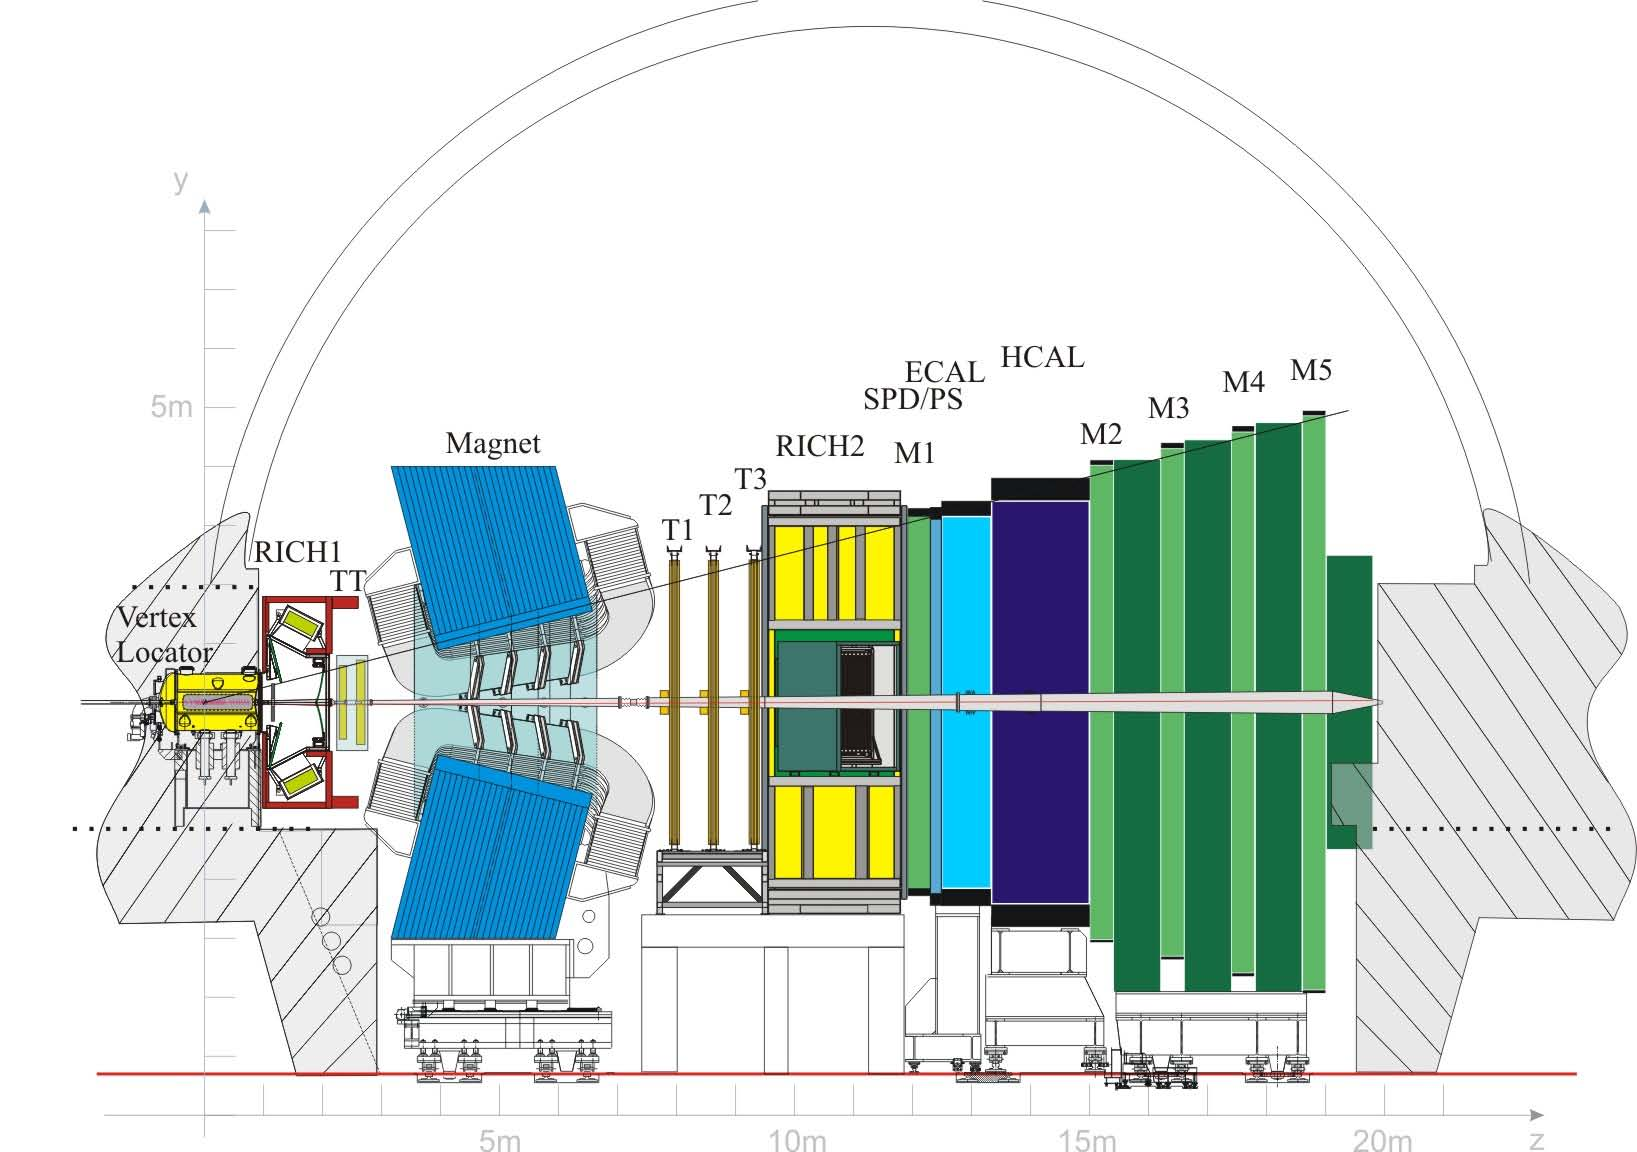
\includegraphics[width=\columnwidth]{Chapters/detector/images/lhcb_schematic.jpg}
	\caption{LHCb schematic}
	\label{fig: lhcb_schematic}
\end{figure}

% DETECTOR ACEPTANCE
%Figure \ref{} shows the momentum distribution for $\pi^+ \pi^-$ pairs from the decay of $B_d^0$ particles. Overlaid are $\pi^+ \pi^-$ pairs which have been reconstructed within the LHCb detector and $\pi^+ \pi^-$ pairs that have not. Events are produced by the PYTHIA event generator.  The decrease in detector acceptance at low momenta is due to slow pions that do not hit enough tracking stations for their momenta to be measured. This is due to the magnet bending the path of low momenta pions outside the detector acceptance. At high momenta the decrease in detector acceptance is due to particles with trajectories that are within the beam pipe.

\section{Vertex Locator (VELO)}
\label{section: velo}
%=========================================================================%
%=============================  Vertex reconstruction  ==========================%
%=========================================================================%
%The properties of these decays such as the decay position, lifetime of the B/D mesons and their  products need also to be highly accurate in order to minimise the uncertainty on the key measurements at the LHCb experiment.  
%Particle interactions are characterised by particles originating from a common point in space. With the presence of interacting particles In the case of particle production or with the association of a single parent particle in interactions involving decays.
%
%Since the focus of the LHCb experiment is the observation of rare decays it follows that the detector be optimised such that 
%
%The position of beam proton-proton interactions and particle decays are described by a vertex. A vertex provides information on the position of the event and the particles produced as a result. The identification, positional accuracy of vertices along with the correct association of interactions to their product particles is fundamental in achieving the physics goals of the LHCb experiment, its presence in an event serves as a clear indicator of the rare physics processes that are the focus of the LHCb detector. 
%
%Unique to the LHCb detector.
%
%Vertex reconstruction of interaction points and decay vertices is an extremely important aspect of the LHCb experiment. This is due to the primary focus of the experiment being around the analysis of rare decay processes. From this is follows that the LHCb detector must have good tracking around the interaction region such that a vertex which has been inferred from the direction of the tracks has a small error on its position and i.e. decay lifetime. In addition to this accurate tracking is required in order to accurately measure the impact parameter of tracks, an important input for the trigger.

%Particle interactions are characterised by particles originating from a common point in space. With the presence of interacting particles In the case of particle production or with the association of a single parent particle in interactions involving decays.
%
%Since the focus of the LHCb experiment is the observation of rare decays it follows that the detector be optimised such that 
%
%The position of beam proton-proton interactions and particle decays are described by a vertex. A vertex provides information on the position of the event and the particles produced as a result. The identification, positional accuracy of vertices along with the correct association of interactions to their product particles is fundamental in achieving the physics goals of the LHCb experiment, its presence in an event serves as a clear indicator of the rare physics processes that are the focus of the LHCb detector. 
%
%Unique to the LHCb detector.
%
%Vertex reconstruction of interaction points and decay vertices is an extremely important aspect of the LHCb experiment. This is due to the primary focus of the experiment being around the analysis of rare decay processes. From this is follows that the LHCb detector must have good tracking around the interaction region such that a vertex which has been inferred from the direction of the tracks has a small error on its position and i.e. decay lifetime. In addition to this accurate tracking is required in order to accurately measure the impact parameter of tracks, an important input for the trigger.
%To achieve this the LHCb detector has a dedicated vertex reconstruction sub-detector called the VELO detector. The VELO detector is made up of a series of silicon stations which are positioned along the direction of the beam (Fig \ref{fig: VELO_silicon_stations}). Each station is segmented into two halves such that the two halves of the VELO can through a mechanical system move into open and closed configurations(Fig \ref{fig: VELO layout}).
%
%This mechanism enables the VELO detector to maximise its resolution by minimising the distance between the nominal interaction region and the sensitive areas of the VELO. During periods of stable beam the minimum distance between the nominal interaction region and the sensitive area of the VELO detector is $ \approx 5mm$. However during the process of beam injection the width of the beam can be greater. To protect the components of the VELO during this process the two halves of the VELO are separated by as much as $6mm$.

%\begin{itemize}
%	\item Station layout
%	\item r-$\phi$ sensors
%	\item pile-up sensors and L0 trigger
%	\item LHC vacuum and VELO vacuum
%	\item RF foils
%\end{itemize}

%1. VELO motivation
%2. VELO features and layout
%3. VELO performance

The detection of rare B and D meson decays is a key requirement to meet the physics goals of the LHCb experiment.  In the LHCb detector these processes are characterised by the presence of production and decay vertices. To maximise the sensitivity of detecting and correctly identifying these events via the presence of displaced vertices a dedicated sub-detector system called the VELO (Vertex locator) is employed around the nominal interaction region. The detection of vertices is achieved indirectly via the detection of their decay products through track reconstruction, the paths of which are extrapolated towards a common point of intersection to give the vertex. The reconstruction of VELO tracks is also important for use in the LHCb trigger system, discussed in section \ref{section: trigger}.

The VELO is a silicon micro strip vertex detector, it is made up of two halves (left and right) each containing twenty one track station modules (figure \ref{fig: VELO_silicon_stations}) positioned at different points along the beam axis. The angular coverage of the VELO detector is shown in figure \ref{fig: velo angular acceptance}.

\begin{figure}
	\centering
	\includegraphics[width=0.5\columnwidth]{/Users/admin/Dropbox/LHCb/detector/VELO/images/silicon_stations.jpg}
	\caption{VELO silicon stations during partial construction of the VELO sub-detector}
	\label{fig: VELO_silicon_stations}
\end{figure}

\begin{figure}
	\centering
	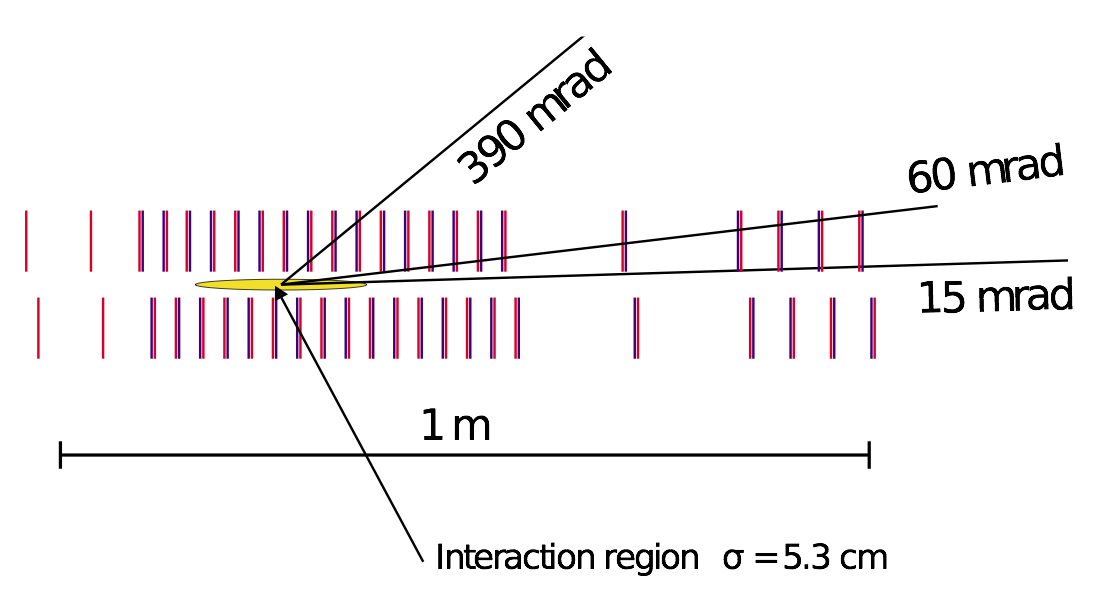
\includegraphics[width=0.7\columnwidth]{Chapters/detector/images/velo_angular_acceptance.png}
	\caption{The layout of the VELO R (red) and $\phi$ (blue) sensors shown in the (x,z) plane. A $\pm2\sigma$ area around the nominal interaction point is shown in yellow. Lines drawn at 390 mrad and 15 mrad represent the maximum and minimum angular coverage, while the line at 60 mrad shows the average track angle in minimum bias events. The left-most two pairs of R sensors are the pileup veto stations.}
	\label{fig: velo angular acceptance}
\end{figure}

Modules are approximately semi-circular in shape, 300 \,$\mu$m thick, with an outer diameter of 84 mm and an inner diameter of 8mm in order to accommodate the beam pipe. Each module is composed of a pair of sensors which measure the radial distance and azimuthal angle of particles traversing the detector. The silicon strips of the radial sensor are orientated radially about the module and in concentric semi-circles for the azimuthal sensor, see figure \ref{fig: r-phi sensors}. The modules are also contained within a secondary vacuum to reduce background contributions from interactions with gas particles in the beam pipe, this is enclosed by a 300$\mu$m thick aluminium foil which also protects from radio frequency pickup from the beam.

\begin{figure}
	\centering
	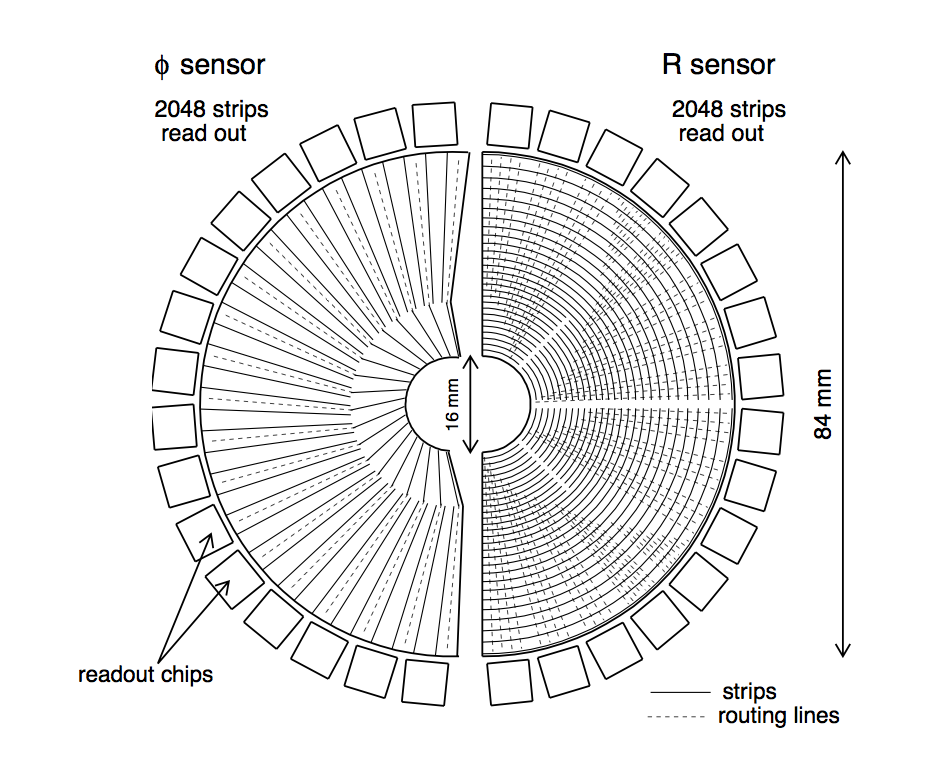
\includegraphics[width=0.5\columnwidth]{Chapters/detector/images/r-phi_sensors.png}
	\caption{Schematic diagram of a VELO station from the perspective of along the beam line. Each half consists of both R and $\phi$ sensors though in this figure only the $\phi$ sensors are shown in the left half and only the R sensors are shown in the right half.}
	\label{fig: r-phi sensors}
\end{figure}

The two halves of the detector open and close about the interaction region depending on the status of the LHC beam (see fig \ref{fig: VELO layout}). During the beam fill or dumping the VELO is put into its open configuration in order to minimise radiation damage to its components. When the beam is stable the VELO is configured into its closed configuration (In this configuration the minimal distance between the silicon trackers and the beamline is 8mm) to maximise its tracking resolution.

\begin{figure}
	\centering
	\includegraphics[width=\columnwidth]{/Users/admin/Dropbox/LHCb/detector/VELO/images/VELO_open_closed.png}
	\caption{The front face of the first modules illustrated in two configurations. Closed (left): Once the beam position is stable the halves close so that the position between the VELO and the interaction region is minimised. Open: The two halves are separated in order to protect the modules from the unstable beam.}
	\label{fig: VELO layout}
\end{figure}

Figure \ref{fig: pv resolution} shows the resolution of the primary vertex position as a function of track multiplicity and figure \ref{fig: ip resolution} shows the resolution of the impact parameter as a function of $p_\mathrm{T}^{-1}$. Both of these measurements approach the expected design parameters \cite{Latham:1491236}.

%The VELO reconstructs vertices with a resolution of $\sim10\,\mu$m; this corresponds to a $\sim40$ fs resolution in the measurement of particle lifetimes and an impact parameter resolution of $20\,\mu$m. %Reconstructs particles from $15$ mrad to $390$ mrad.

\begin{figure}[h]
	\centering
	\begin{subfigure}[b]{0.45\textwidth}
		\includegraphics[width=\columnwidth]{/Users/admin/Dropbox/LHCb/detector/VELO/images/pv_resolution_xy.png}
		\caption{x in red, y in blue}
	\end{subfigure}
	\begin{subfigure}[b]{0.45\textwidth}
		\includegraphics[width=\columnwidth]{/Users/admin/Dropbox/LHCb/detector/VELO/images/pv_resolution_z.png}
		\caption{z}
	\end{subfigure}
	\caption{Resolution of primary vertex position}
	\label{fig: pv resolution}
\end{figure}

\begin{figure}[h]
	\centering
	\includegraphics[width=\columnwidth]{/Users/admin/Dropbox/LHCb/detector/VELO/images/ip_resolution.png}
	\caption{Impact parameter resolution as a function of $p_T^{-1}$}
	\label{fig: ip resolution}
\end{figure}


\section{Ring Imaging Cherenkov Detectors (RICH)}
\subsection*{Cherenkov Radiation}
Charged particles traversing through a medium at a speed greater than the speed of light in the same medium emit electromagnetic radiation known as Cherenkov radiation. The angle at which the radiation is emitted relative to the direction of the particle (Cherenkov angle, $\theta_C$) is constant given the speed of the particle and the refractive index of the medium are also constant. The relationship between the speed of the particle ($\beta = |\vec{v}|/c$), refractive index of the medium ($n$) and the Cherenkov angle ($\theta_C$) is described by the equation,

\begin{equation}
	\cos{\theta_C} = \frac{1}{n\beta}\\
	\label{equation: Cherenkov radiation}
\end{equation}

The speed of the particle, $\beta$ can be expressed in terms of its mass $m$ and momentum $\vec{p}$, the equation for the Cherenkov angle in these terms is then,

\begin{equation}
	\cos{\theta_C} = \frac{1}{n}\sqrt{1 + \frac{m^2}{p^2}}
	\label{equation: Cherenkov angle in terms of mass and momentum}
\end{equation}

where $\beta=\frac{|\vec{p}|}{E} = \frac{|\vec{p}|}{\sqrt{p^2 + m^2}} = \frac{1}{\sqrt{1 + m^2/p^2}}$. For a charged particle emitting Cherenkov radiation, measurements of the Cherenkov angle of its emitted photons together with its momentum information (e.g. using information from tracking systems) and the above relationship allows the calculation of its mass and hence particle type (particle and anti-particles can be distinguished by their charge, e.g from the direction of bend when passing through a magnetic field). Measurements of the Cherenkov angle in the LHCb detector are achieved through its RICH system. 

%$|\vec{p}|\sqrt{(n^2 cos^2(\theta_C) - 1)}$

%\begin{eqnarray}
%	\beta&=&\frac{|\vec{p}|}{E}
%	= \frac{|\vec{p}|}{\sqrt{\vec{p}^2 + m^2}}
%	= \frac{1}{\sqrt{1 + m^2/\vec{p}^2}}
%	= \frac{\gamma m |\vec{v}|}{\gamma m} \,\,\,\,\,\,\,\,\,\,\,\,\,\,\,\,\,\,\,\, c = 1
%\end{eqnarray}

%It detects charged particles via their Cherenkov radiation emitted when traversing a medium of refractive index $n$ faster than the speed of light in the same medium
\subsection*{Requirements of the RICH detector}
%The RICH system is a key component in the LHCb particle identification system; it is 
The RICH is designed to provide excellent discrimination between charged hadrons, in particular, pions, kaons, and protons (though identification of charged leptons is also possible). This allows the discrimination between different hadronic decays, in particular, processes with similar topologies but different final states e.g. $B^0 \rightarrow h^+h^-$ \cite{JHEP10(2012)037} (figure \ref{fig: inv_mass_b_to_hh}), $B_c^+ \rightarrow J/\psi \pi^+\pi^-\pi^+$ \cite{PhysRevLett.108.251802},  $B^+ \rightarrow DK^+$ \cite{Aaij2012203}, $B^0\rightarrow K^{*0}\gamma$ \cite{PhysRevD.85.112013} and $B_s^0 \rightarrow K^\pm \pi^\mp$ \cite{PhysRevLett.108.201601}.

\begin{figure}[htbp]
	\begin{center}
		\begin{subfigure}[b]{0.49\textwidth}
			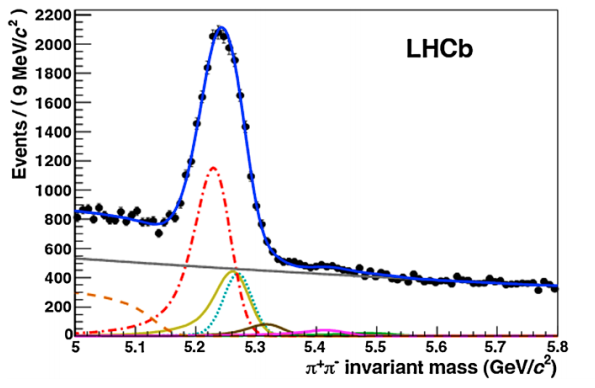
\includegraphics[width=\textwidth]{./Chapters/detector/rich/inv_mass_b_to_hh_no_rich.png}
			\caption{Without RICH information}
			\label{fig: inv_mass_b_to_hh_no_rich.png}
		\end{subfigure}
		\begin{subfigure}[b]{0.49\textwidth}
			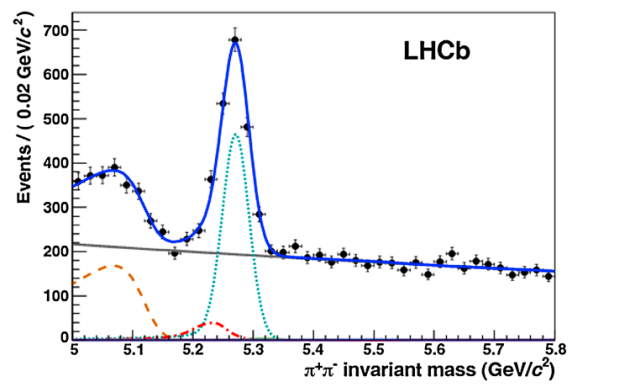
\includegraphics[width=\textwidth]{./Chapters/detector/rich/inv_mass_b_to_hh_with_rich.png}
			\caption{With RICH information}
			\label{fig: inv_mass_b_to_hh_with_rich.png}
		\end{subfigure}
		\caption{Invariant mass distribution of $B\rightarrow h^+h^-$ decays before (A) and after (B) inclusion of RICH information to isolate the signal decay, $B^0 \rightarrow \pi^+\pi-$ (teal dashed). The background processes are $B^0\rightarrow K\pi$ (red dashed-dotted), $B^0 \rightarrow$ 3-body (orange dashed), $B_s \rightarrow KK$ (yellow), $B_s \rightarrow K\pi$ (brown) $\Lambda_b \rightarrow pK$ (purple) and $\Lambda_b \rightarrow p\pi$~(green). There is also a contribution from combinatorial background (grey).}
		\label{fig: inv_mass_b_to_hh}
	\end{center}
\end{figure}

In addition to the discrimination between exclusive decay processes, information from the RICH detector is also used to make more general decisions on whether an event is of interest e.g. identification of events with at least one $\phi$ particle (which are present in many decay modes of interest). These decisions require significantly less CPU processing than exclusive event selection such that they are well suited to the strict time constraints of the trigger system, see section \ref{section: trigger}.

In a addition to direct processes (where the charged hadron identified is part of the processes being investigated) the particle identification also provides a method of flavour tagging in measurements of CP asymmetries or particle anti-particle oscillations. Such particles which are used to tag events typically have lower transverse momenta than particles from the decay of heavy B mesons. In order to satisfy the requirements stated previously the RICH must maintain good performance over a large range of momenta (2-100 GeV/c \cite{JHEP10(2012)037}).

\subsection*{Detector Description}

The RICH system consists of two RICH detectors, RICH1 and RICH2 \cite{Amato:494263}. RICH1 is positioned directly downstream of the Vertex Locator (VELO) and upstream of the magnet; it is attached directly to the VELO exit window. RICH2 is positioned downstream of the magnet and Tracking stations (T1, T2 and T3). They are approximately 1 m and 10 m downstream of the nominal interaction interaction point respectively (see figure \ref{fig: lhcb_schematic}), cover an angular acceptance of $\pm(25-300)$ [$\pm(15-120)$] mrad and momentum range of $2-40$ [$15-100$] GeV/c see figure \ref{fig: rich_angular_and_momentum_coverage}.

In order for Cherenkov radiation to occur a medium with a refractive index $n>1$ is required. The RICH system employs three different mediums (in the context of RICH detectors these are more commonly referred to as radiators) in order to cover the desired momentum range, see figure \ref{fig: radiators}. RICH1 contains both an aerogel and $\mathrm{C}_4\mathrm{F}_{10}$ gas whilst RICH2 contains only $\mathrm{CF}_4$ gas. The refractive indices of these are 1.03, 1.0014 and 1.0005 (at $0^\circ$, $101$ kPa and for photons with a wavelength of 400 nm) respectively.

\begin{figure}[htbp]
	\begin{center}
		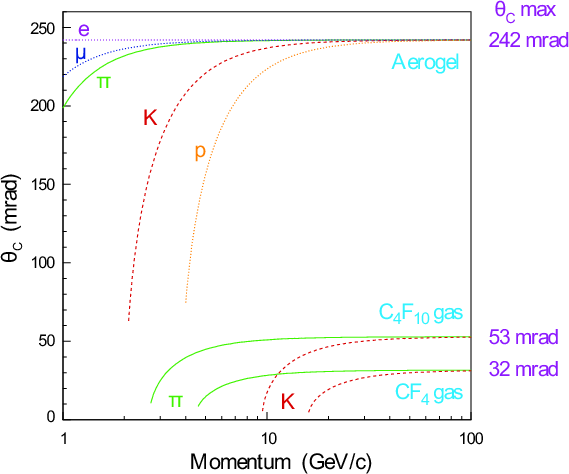
\includegraphics[width=0.6\textwidth]{./Chapters/detector/rich/radiators.png}
		\caption{Cherenkov angle $\theta_C$ as a function of particle momentum, particle type and radiator type.}
		\label{fig: radiators}
	\end{center}
\end{figure}


\begin{figure}[htbp]
	\begin{center}
		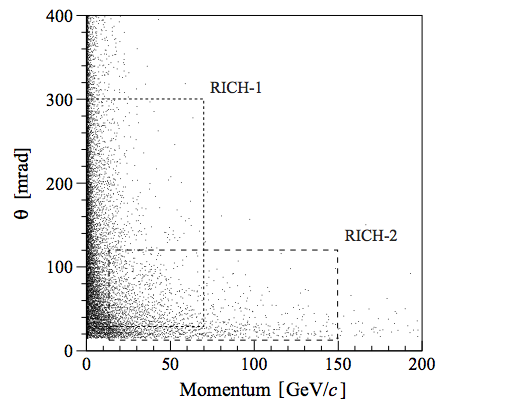
\includegraphics[width=0.6\textwidth]{./Chapters/detector/rich/rich_angular_and_momentum_coverage.png}
		\caption{Polar angle $\theta$ and momentum $p$ distribution of the tracks in simulated $B^0\rightarrow \pi^+\pi^-$ decays. The angular coverage and momentum range or the RICH detectors are shown by the regions contained in the dotted lines.}
		\label{fig: rich_angular_and_momentum_coverage}
	\end{center}
\end{figure}

Cherenkov photons emitted by charged particles passing through the radiators in the RICH detectors are emitted at a constant angle relative to the direction of the charged particle, this is referred to as the Cherenkov angle, $\theta_C$. Focusing these photons onto a plane with a parabolic mirror results in rings of photons in which the Cherenkov angle can be calculated from the radius. Both RICH detectors employ similar mirror systems; using a spherical mirror to focus the rings and a plane mirror to reflect the rings onto a plane of photon detectors, see figure \ref{fig: rich_system_schematic}. The purpose of the plane mirrors is to direct photons away from the detector where space limitations, radiation and strong magnetic fields create an undesirable environment for the operation of photon detectors. Each of the mirrors are composed of segments, see table \ref{tab: mirror_segmentation} and figure \ref{fig: mirror_segmentation_rich2}

\begin{figure}[htbp]
	\begin{center}
		\begin{subfigure}[b]{0.49\textwidth}
			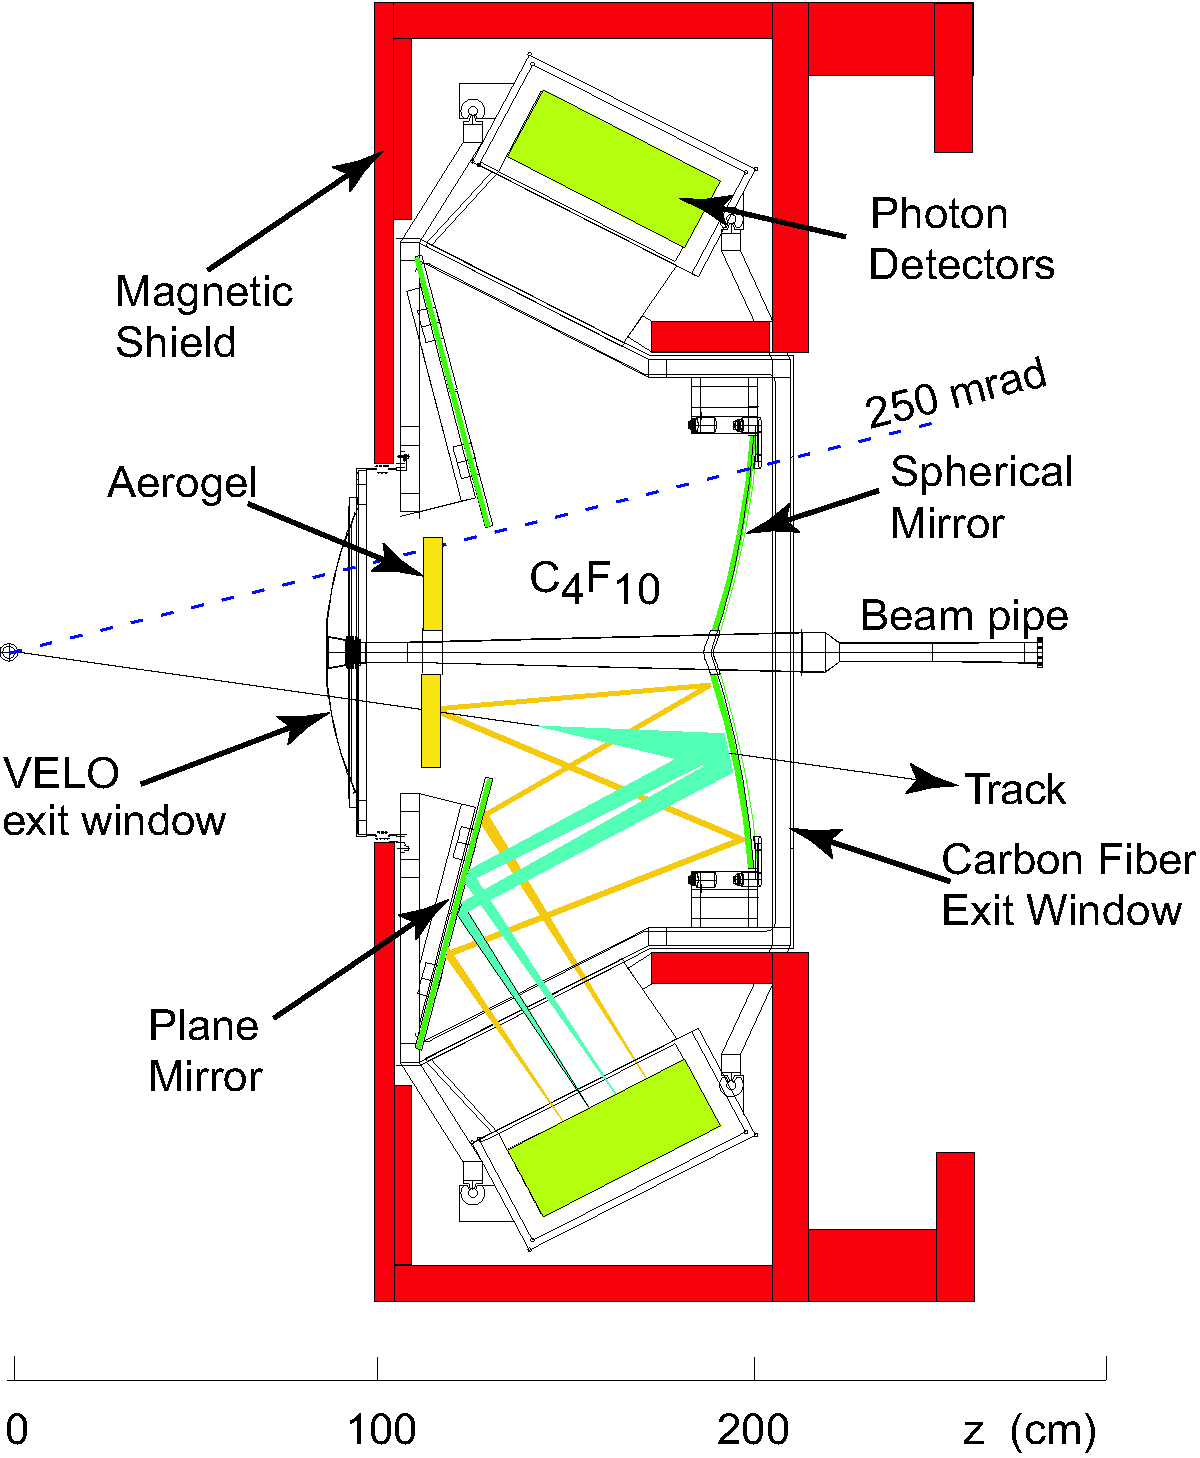
\includegraphics[width=\textwidth]{Chapters/detector/rich/rich1_schematic.png}
			\caption{RICH1, side view}
			\label{fig: rich1_schematic}
		\end{subfigure}
		\begin{subfigure}[b]{0.49\textwidth}
			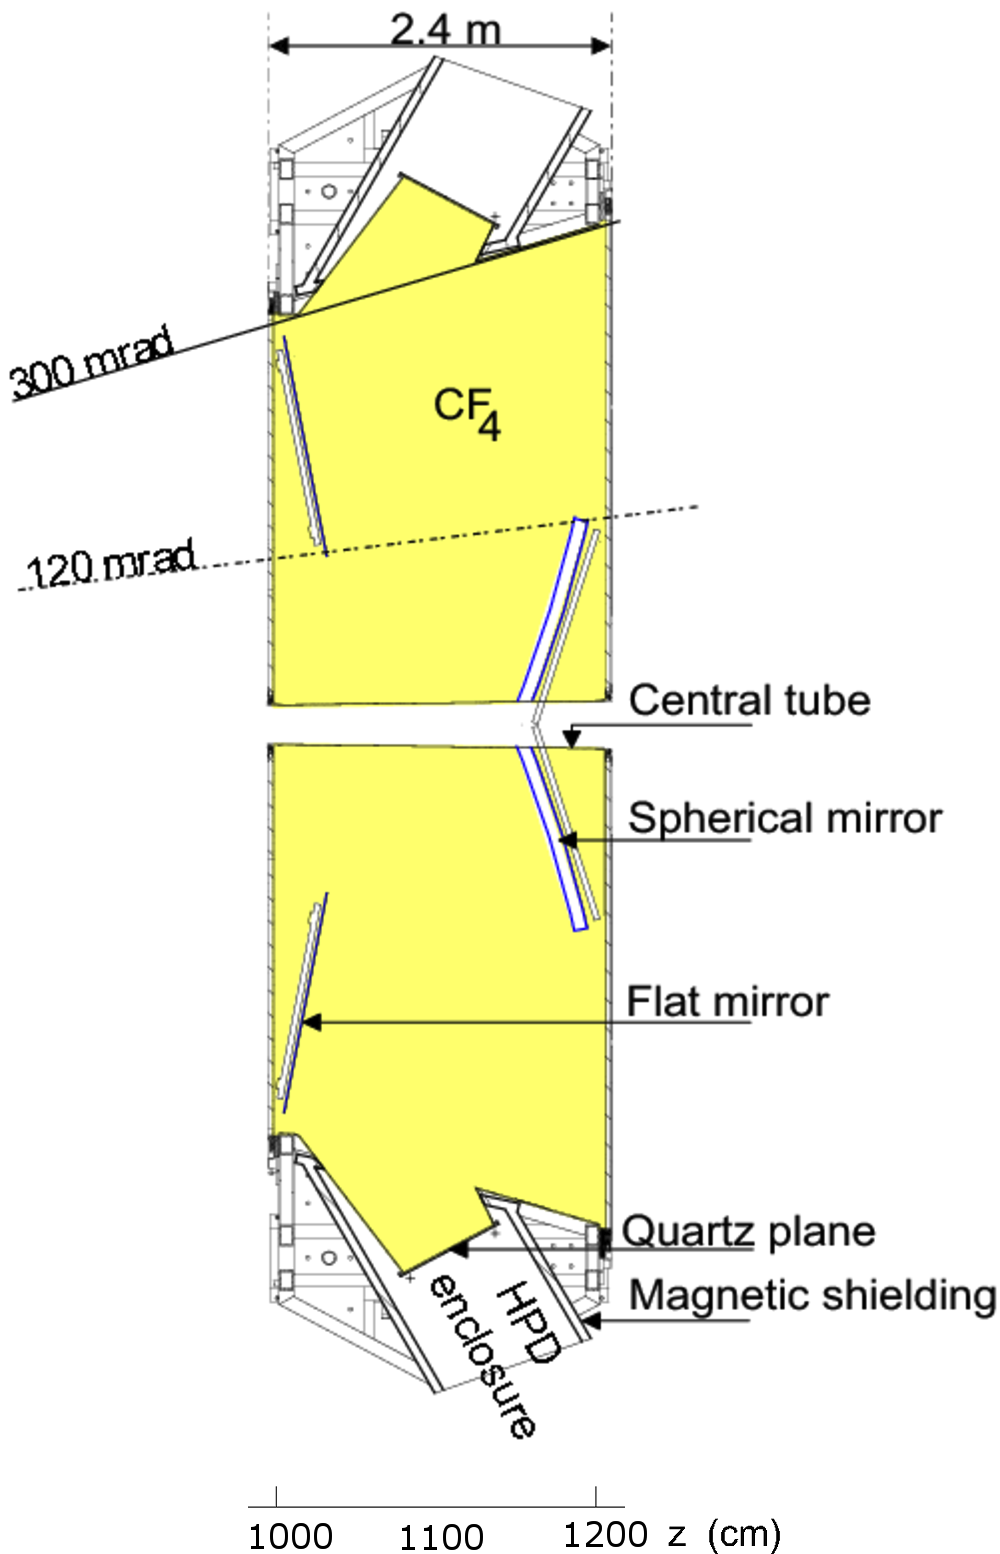
\includegraphics[width=\textwidth]{Chapters/detector/rich/rich2_schematic.png}
			\caption{RICH2, top view}
			\label{fig: rich2_schematic}
		\end{subfigure}
		\caption{Schematic of the RICH detectors, RICH1 (A) and RICH2 (B). The beam pipe runs left to right in both images.}
		\label{fig: rich_system_schematic}
	\end{center}
\end{figure}

\begin{table}[htdp]
	\caption{Spherical and plane mirror segmentation scheme in the RICH detectors.}
	\begin{center}
		\begin{tabular}{|c|c|c|}
			\hline
			& Spherical Mirror Segments & Plane Mirror Segments \\ \hline
			RICH1 & 4 & 16 \\ \hline
			RICH2 & 56 & 40 \\ \hline
		\end{tabular}
	\end{center}
	\label{tab: mirror_segmentation}
\end{table}%

\begin{figure}[htbp]
	\begin{center}
		\begin{subfigure}[b]{0.35\textwidth}
			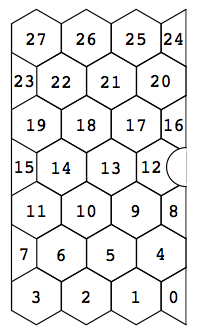
\includegraphics[width=\textwidth]{Chapters/detector/rich/mirror_segmentation_rich2_spherical.png}		
			\caption{}
			\label{}
		\end{subfigure}
		\begin{subfigure}[b]{0.35\textwidth}
			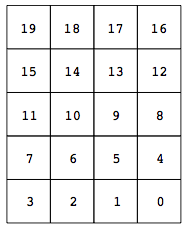
\includegraphics[width=\textwidth]{Chapters/detector/rich/mirror_segmentation_rich2_plane.png}
			\caption{}
			\label{}
		\end{subfigure}
		\caption{Schematic of the spherical (A) and plane (B) mirror segments for the left half of the RICH2 detector. Also shown is the numbering scheme used}
		\label{fig: mirror_segmentation_rich2}
	\end{center}
\end{figure}

The photon detector planes are arrays containing Hybrid Photon detectors (HPDs). There are two planes per RICH detector; Up and Down boxes in RICH1 (containing additional magnetic shields due to their proximity to the magnet) and the Left and Right boxes in RICH2, see figure \ref{fig: rich_system_schematic}. There are a total of 484 HPDs in the RICH system with 196 of them in the RICH1 detector and 288 in the RICH2 detector. 

The entrance to the HPDs consists of a quartz entrance window with a photocathode layer painted on the inner side of the window (see figure \ref{fig: hpd_schematic}). Photons incident on an HPD stimulate the emission of electrons into a vacuumed cavity inside the HPD via the photocathode layer. These electrons are then accelerated by an electric field across a potential difference of 16 kV onto a 32 x 32 silicon chip array with a pixel size of 2.5 mm x 2.5 mm. The chip records the position of the electron which is used to reconstruct the track of the photon from its emission point in the radiator to photocathode layer on the HPD entrance window. The Cherenkov angle can then be calculated by coupling the photon to its corresponding charged particle and calculating the relative angle between the two.

\begin{figure}[htbp]
	\begin{center}
		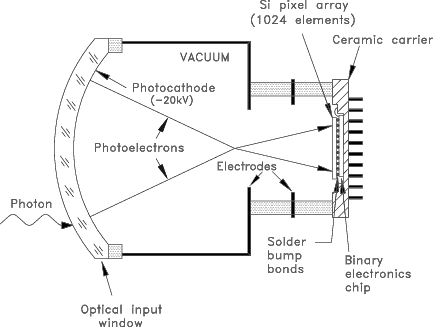
\includegraphics[width=0.6\textwidth]{./Chapters/detector/rich/hpd_schematic.png}
		\caption{Schematic diagram of a Hybrid Photon Detector (HPD)}
		\label{fig: hpd_schematic}
	\end{center}

\end{figure}

\subsubsection*{Performance - Cherenkov Angle Resolution}
For a medium with refractive index $n$ and where $|\vec{p}| >> m$ the Cherenkov angle becomes \emph{saturated} such that for all particle types the Cherenkov equation (equation \ref{equation: Cherenkov angle in terms of mass and momentum}) can be expressed as,

\begin{equation}
	\cos{\theta_C^{max}} = \frac{1}{n}
	\label{equation: saturated Cherenkov radiation}
\end{equation}

such that the Cherenkov angle for all particle types converge,

\begin{equation}
	\theta_C^{max}(\pi) = \theta_C^{max}(K) = \theta_C^{max}(p)
\end{equation}

\emph{Saturation} of the Cherenkov angle in the LHCb RICH detector can be seen in the high momentum regions of figure \ref{fig: radiators}. The saturation Cherenkov angles are 242 mrad, 53 mrad and 32 mrad for the Aeorogel $\mathrm{C}_4\mathrm{F}_{10}$ and $\mathrm{CF}_4$ radiators respectively. The alignment of the RICH detector can then be tested by plotting the distribution of the difference between the measured Cherenkov angle and the saturated Cherenkov angle, $\Delta\theta_C = \theta_C$ - $\theta_C^{max}$ for photons emitted from saturated tracks.%; %if the detector is perfectly aligned then this distribution will be described by a delta function, $\delta(\Delta\theta)$.

%\subsubsection*{Performance - Particle Identification} edit
\section{Magnet}
\label{section: magnet}

A dipole magnet is present for momentum determination of charged particles. The magnet provides an integrated downstream field of $3.6$ Tm which results in a momentum resolution better than $\delta p / p \approx 0.5\%$ for tracks with momentum less than 200 GeV \cite{Amato:424338}. The magnet is positioned after the VELO and RICH 1 sub detectors so that the magnetic field does not effect the vertex reconstruction and particle identification of low momentum particles. The structure of the magnet is designed such that the magnetic field does not disrupt the components of other sub-detectors such as the Photon detectors in the RICH systems which use large electric fields. The field lines of the dipole magnet result in a predominantly horizontal Lorentz force on the charged particles in the LHCb detector, consequently tracks are predominantly bent in this plane.
\section{Tracking}
\label{section: tracking}

The LHCb tracking system consists of the VELO; the Tracker Turicensis (TT) and the T1, T2 and T3 detectors (collectively called the T-stations), see figure \ref{fig: lhcb_schematic}. 

\subsection{Tracker Turicensis (TT)}
The Tracker Turicensis is located before the magnet and after the VELO detector. In addition to charged particles produced in the VELO detector the location of the TT allows it to provide tracking information for charged particles produced from the decay of long lived neutral particles such as the $K_S^0$ which may not decay in the VELO detector. It also provides tracking information for charged particles with low momentum which may not reach the T-stations downstream of the magnet due to the bending of then magnet.

The TT is a silicon micro strip detector with height of 1.5 m and width of 1.3 m, covering the full angular acceptance of the LHCb detector. It consists of 4 layers, the first and last are made up of vertical strips, the second and third inner layers have strips which have been rotated by 5 $^\circ$ and -5 $^\circ$ stereo angle to provide the transverse position of particles.

\begin{figure}
	\centering
	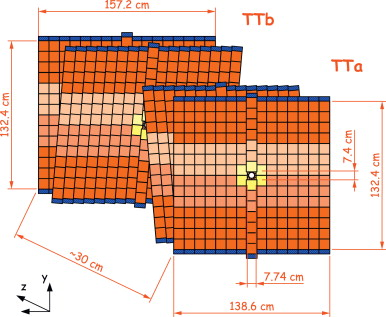
\includegraphics{Chapters/detector/images/tracker_turicensis_schematic.jpg}
	\caption{Layout of the 4 stations which constitutes the Tracker Turicensis}
	\label{fig: trigger turicensis schematic}
\end{figure}

\subsection{T-Stations T1, T2 and T3}

The T-stations are positioned after the magnet (see figure \ref{fig: lhcb_schematic}). Together with the tracking detectors upstream of the magnet the trajectory of charged particles through the magnetic field can be measured. The Lorentz force causes the trajectory of charged particles to bend as it traverses the magnetic field; from this the momentum of the track can be measured.

\subsection{Track Reconstruction}
\label{subsection: tracking, track reconstruction}

Track reconstruction at the LHCb detector is carried out via several different tracking strategies; generally these involve reconstructing tracks at the sub-detector level called track segments. For example tracks may be reconstructed purely from hits in the VELO sub-detector, these are known as VELO tracks. Similarly tracks may be reconstructed only from hits in the T-stations positioned downstream of the LHCb magnet. These segments may then be combined with hits in other trackers or other track segments to give a more detailed description of the corresponding particle. For example a VELO track segment may be combined with hits from the TT tracker to give an Upstream track, similarly a T-station track segment may also be combined with hits in the TT tracker to give a Downstream track. The possible track types are outline in figure \ref{fig: track types} and a more detailed description of each of the strategies can be found at \cite{lhcb_track_strategies}.

\begin{figure}[h]
	\centering
	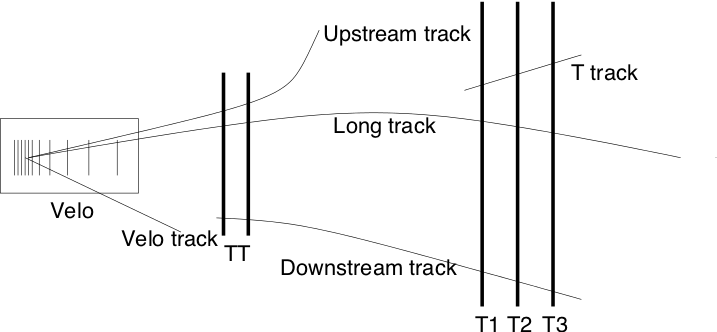
\includegraphics[width=0.8\textwidth]{/Users/admin/Dropbox/PhD/Thesis/Chapters/detector/tracking/images/tracktypes.png}
	\caption{LHCb Track Types}
	\label{fig: track types}
\end{figure}

\section{Calorimeter}

The calorimeter system fulfils several primary roles in the LHCb detector. It provides very fast measurements which are used by the trigger to make quick judgements on an event (a decision is made 4 microseconds after the interaction); examples of such measurements are,

\begin{itemize}
	\item $E_T$ of electrons, photons and neutral pions 
	\item $E_T$ and $\Sigma(E_T)$ of Hadrons
\end{itemize}

As well as providing fast information it also provides information on the particle type, discriminating between electrons, photons and hadrons. It is especially useful at identifying neutral particles such as photons and neutral mesons, e.g. pions. This enables the LHCb detector to make  physics measurements for many decays, see table \ref{table: calorimeter processes},
\\
\begin{table}[h]
	\begin{center}
		\begin{tabular}{ |l|l| }
		%	\hline
		%	\multicolumn{2}{ |c| }{Calorimeter Particle Identification} \\
			\hline
			Particle Type & Example Process \\ \hline
			Electron & $B \rightarrow K* e^+ e^-$ \\ \hline
			\multirow{2}{*}{Photons} & $B_d \rightarrow K* \gamma$ \\
				 & $B_s \rightarrow \phi \gamma$ \\ \hline
			\multirow{2}{*}{Neutral Mesons} & $B_d \rightarrow \pi^+\pi^-\pi^0$ \\
				 &  $B_d \rightarrow J/\psi \eta$ \\ \hline
		\end{tabular}
		\caption{Calorimeter particle identification}
		\label{table: calorimeter processes}
	\end{center}
\end{table}

The calorimeter system is positioned approximately thirteen metres downstream of the nominal interaction point with a solid angle coverage of 300 mrad in x and 250 mrad in y \cite{Amato:494264}. It extends for 2.7 metres (See figure \ref{fig: lhcb_schematic}) and is composed of several sub-components. In order of distance from the nominal interaction point these are the Scintillating Pad Detector (SPD), a 2.5 radiation length ($2.5\,X_0 = 12$~mm) lead wall, the Pre Shower (PS), an electromagnetic calorimeter (ECAL) with dimensions of 4 m x 3.5 m and a hadronic calorimeter (HCAL). Each component is designed to maximise the signal of certain particle types and minimise the signal for others. The nominal signal deposition regions for various particle types are shown in figure \ref{fig:animals}

\begin{figure}[h]
        \centering
        \begin{subfigure}[b]{0.5\textwidth}
                \centering
                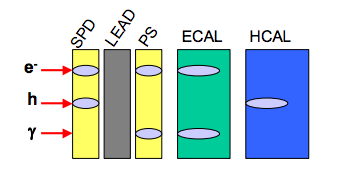
\includegraphics[width=\textwidth]{./Chapters/detector/calorimeter/deposition_region.png}
                \label{fig: calo_nominal_detection_regions1}
                \caption{}
        \end{subfigure}
        \begin{subfigure}[b]{0.4\textwidth}
                \centering
                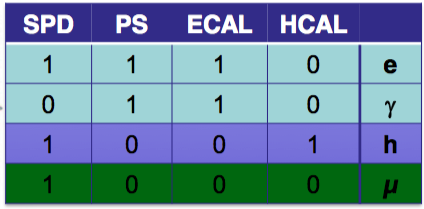
\includegraphics[width=\textwidth]{./Chapters/detector/calorimeter/deposition_region_table.png}
                \label{fig: calo_nominal_detection_regions2}
                \caption{}
        \end{subfigure}
        \caption{(A): Nominal regions of energy deposition in the LHCb calorimeter system for various particle types (B): Nominal particle signal detection in the LHCb calorimeter system for various particle types}
        \label{fig:animals}
\end{figure}

\begin{figure}[h]
	\centering
	\begin{subfigure}[b]{0.45\textwidth}
		\centering
		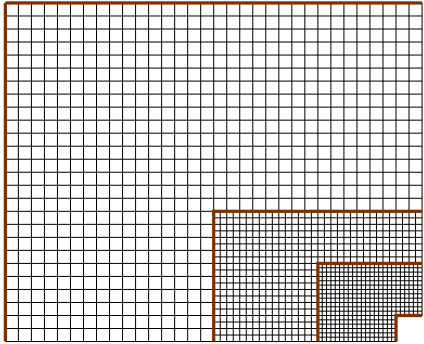
\includegraphics[width=\textwidth]{./Chapters/detector/calorimeter/ecal_graularity.png}
		\caption{ECAL}	
		\label{fig: ECAL granularity}
	\end{subfigure}
	\begin{subfigure}[b]{0.45\textwidth}
		\centering
		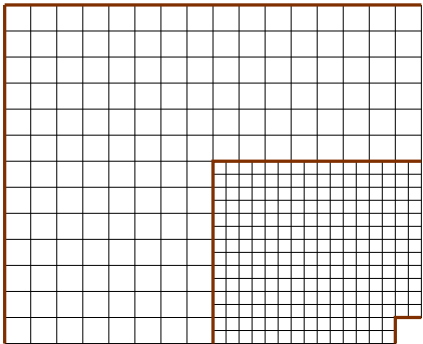
\includegraphics[width=\textwidth]{./Chapters/detector/calorimeter/hcal_granularity.png}
		\caption{HCAL}	
		\label{fig: HCAL granularity}
	\end{subfigure}
	\caption{Schematic of the cell granularity of the LHCb calorimeters for one of its quadrants. See tables \ref{table: Calorimeter details} and \ref{table: Calorimeter details2} for further details.}
\end{figure}

\begin{table}[htdp]
	\caption{Cell granularity structure of the SPD/PS and ECAL components of the LHCb calorimeter system}
	\begin{center}
		\begin{tabular}{|c|c|c|c|}
			\hline
			& Inner region & Middle region & Outer region \\
			\hline
			Cell size (mm) & 40.4 & 60.6 & 121.2 \\
			\hline
			Number of channels & 1472 & 1792 & 2688 \\
			\hline
		\end{tabular}
	\end{center}
	\label{table: Calorimeter details}
\end{table}%

\begin{table}[htdp]
	\caption{Cell granularity structure of the HCAL component of the LHCb calorimeter system}
	\begin{center}
		\begin{tabular}{|c|c|c|}
			\hline
			& Inner region & Outer region \\
			\hline
			Cell size (mm) & 131.3 & 262.6 \\
			\hline
			Number of channels & 860 & 680 \\
			\hline
		\end{tabular}
	\end{center}
	\label{table: Calorimeter details2}
\end{table}%


The SPD and PS are made from scintillator pads and contain a groove which holds a helicoidal optical fibre that collects scintillating light. The ECAL is a Shashlik electromagnetic calorimeter, it is made of interleaved tiles of 2mm think lead absorbers and 4mm thick scintillator material orientated to face the direction of the beam pipe; there are 66 of these interleaved pairs of lead and scintillator tiles giving a longitudinal size of 25 radiation lengths ($X_0$). The HCAL is made of interleaved plates of Scandium and Iron and is orientated in the horizontal plane. It has a longitudinal size of 5.6 hadron interaction lengths ($\lambda_I$) and is made up of 26 layers of Scandium and Iron plate pairs.

From beam tests \cite{1742-6596-293-1-012052} the ECAL has been shown to have an energy resolution of,
\begin{equation*}
	\frac{\sigma_E}{{E}} = \frac{(8-10)\%}{\sqrt{E}} \oplus 0.9\%
\end{equation*}

and the HCAL has been shown to have a resolution of 
\begin{equation*}
	\frac{\sigma_E}{E} = \frac{69\pm5\%}{\sqrt{E}} \oplus 9\pm2\%
\end{equation*}

%Figure \ref{fig: reconstruction using calorimeter} shows examples of particle reconstruction using information from the calorimeter system.
Figure \ref{fig: reconstruction using calorimeter} shows the invariant masses of particles reconstructed using hits in the calorimeter system.

\begin{figure}
	\centering
	\begin{subfigure}[b]{0.42\textwidth}
		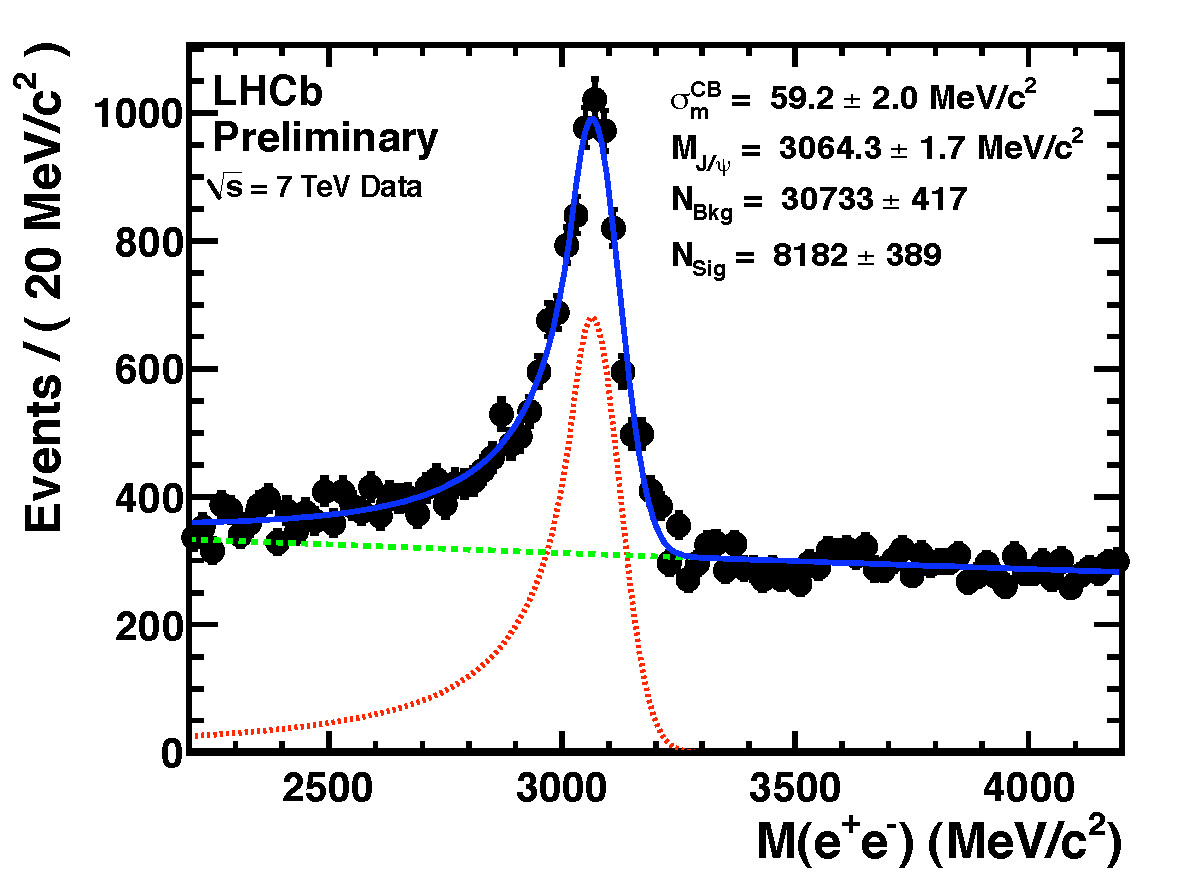
\includegraphics[width=\textwidth]{./Chapters/detector/calorimeter/jpsi_to_ee.pdf}
		\caption{}
	\end{subfigure}
	\begin{subfigure}[b]{0.46\textwidth}
		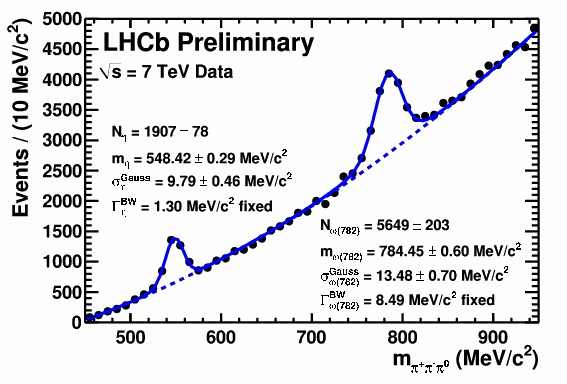
\includegraphics[width=\textwidth]{./Chapters/detector/calorimeter/eta_omega_pipipi_reconstruction.jpg}
		\caption{}
	\end{subfigure}
	\caption{Reconstruction of (A) $J/\psi \rightarrow e^+e^-$} and (B) $\eta/\omega \rightarrow \pi^+\pi^-\pi^0$ using information from the calorimeter system.
	\label{fig: reconstruction using calorimeter}
\end{figure}

\section{Muon System}

Muon detection is an important requirement for the LHCb detector. Muons are present in the final state of many of the key decays that are sensitive to new physics and the rare decays shown in table \ref{table: Muon decays}, They are also used to determine the flavour of neutral B mesons in electroweak and strong processes.% in in $B_{d,s}^0 \rightarrow \mu X$ decays.


%\begin{itemize}
%	\item $B_s^0 \rightarrow \mu^+ \mu^-$ %[First evidence for the decay Bs -> mu+ mu-]}
%	 \item $B \rightarrow J/\psi(\mu^+\mu^-)K_s$ %[Measurement of the isospin asymmetry in $B \to K^{(*)}?^+?^-$ decays]
%	 \item $B_s^0 \rightarrow J/\psi(\mu^+\mu^-)\Phi$ %[Measurement of the CP-violating phase phi_s in the decay Bs->J/psi phi]
% \end{itemize}
% 
% \begin{equation*}
%	B_s^0 \rightarrow \mu^+ \mu^-
%\end{equation*}
% 
% \begin{equation*}
%	B_s^0 \rightarrow \mu^+ \mu^-
%\end{equation*}
% 
% \begin{equation*}
%	B_s^0 \rightarrow \mu^+ \mu^-
%\end{equation*}

\begin{table*}[htdp]
	\caption{}
	\begin{center}
		\begin{tabular}{|c|}
			\hline
			Process \\ 
			\hline
			$B_s^0 \rightarrow \mu^+ \mu^-$ \\
			$B \rightarrow J/\psi(\mu^+\mu^-)K_s$ \\ 
			$B_s^0 \rightarrow J/\psi(\mu^+\mu^-)\Phi$ \\
			\hline
		\end{tabular}
	\end{center}
	\label{table: Muon decays}
\end{table*}%

To reconstruct these types of events at the LHCb bunch crossing rate (which peaks at 40MHz corresponding to a bunch crossing every 25 ns) the muon system employs a fast stand alone muon reconstruction and passes the information to the hardware trigger (see section \ref{section: trigger}) of the LHCb which applies a minimum $p_T$ requirement (1.5 GeV/c for events with a single muon or a geometrical mean of 1.3 GeV/c for the two muons with the highest $p_T$ in the event). Events triggered on this muon requirement make up $\sim40\%$ of the hardware level trigger output; together with data from the calorimeter system this makes up the bulk.

For the LHCb detector to be competitive in the physics analysis of decays such as shown in table \ref{table: Muon decays} a trigger efficiency of $\sim95\%$, muon identification of $\sim90\%$, muon misidentification of $\sim1.5\%$ and muon $p_T$ resolution of $\sim20\%$ is required 
%[Muon TDR 2001]
together with a timing resolution of $\sim25$ ns to match the nominal bunch crossing rate. In addition to this the hardware must be capable of handling the high rates of particles passing through the detector as well as the associated radiation damage.

%\begin{table*}[htdp]
%	\begin{center}
%		\caption{$B\rightarrow \mu X$ background processes at LHCb}
%		\begin{tabular}{|c|}
%			\hline
%			Example Background Processes \\
%			\hline
%			$\pi, K \rightarrow \mu X$ \\
%			Shower particles from the calorimeter system \\
%			Machine background, in particular high energy beam halo muons \\
%			\hline
%		\end{tabular}
%	\end{center}
%	\label{table: muon background}
%\end{table*}%

The Muon System is made up of five stations orientated perpendicularly to the beam axis; these are named M1 through to M5, each consisting of two mechanically independent halves called the A and C side. M1 is positioned before the Pre Shower of the calorimeter system 12.1 m from the nominal interaction point and stations M2-M5 are positioned downstream of the calorimeter system 15.2 m, 16.4 m, 17.6 m and 18.8 m from the interaction point (figure \ref{fig: muon system layout}). Stations M2-M5 are interleaved with 80 cm thick iron absorbers designed to remove hadronic backgrounds giving a longitudinal size of 20 hadron interaction lengths for stations M2-M5 ~\cite{1748-0221-8-02-P02022}. The geometry of the muon stations is projective to the nominal interaction point; the transverse dimensions scale with distance from the nominal interaction point such that the angular acceptance is the same for all muon stations; $\pm 306$mrad in the horizontal plane and $\pm 258$mrad in the vertical plane. 

Each of the muon stations is divided into four rectangular regions, labeled R1-R4 in order of radial distance from the beam axis (Since the geometry of the muon stations is projective to the nominal interaction point the relative sizes of the regions between each station are the same). These are further subdivided into 276 rectangular chambers of varying size depending on in which region the chamber is located (figure \ref{fig: muon region granularity}). The chambers are made up of Multi-Wire Proportional Chambers (MWPC) with the exception of R1 in station M1 which uses triple-GEM detectors(Gas Electron Multiplier) due to higher expected particle rates in this region and the higher levels of radiation tolerance for triple-GEM detectors \cite{muon-second-addemdum}. This gives a total of 1380 chambers providing a detection area of 435 m$^2$.

\begin{figure}[htbp]
	\begin{center}
		\begin{subfigure}[b]{0.45\textwidth}
			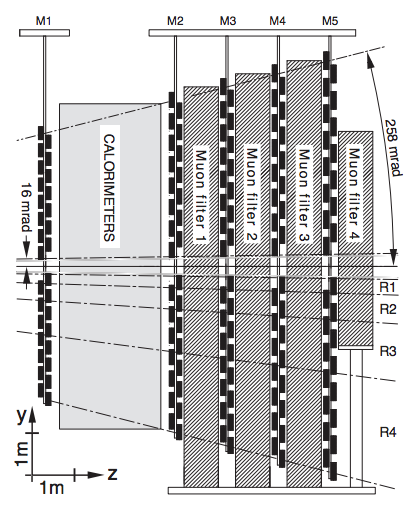
\includegraphics[width=\textwidth]{./Chapters/detector/muon_system/muon_system_side_view.png}
			\caption{Side view of the muon system}
			\label{default}
		\end{subfigure}
		\begin{subfigure}[b]{0.45\textwidth}
			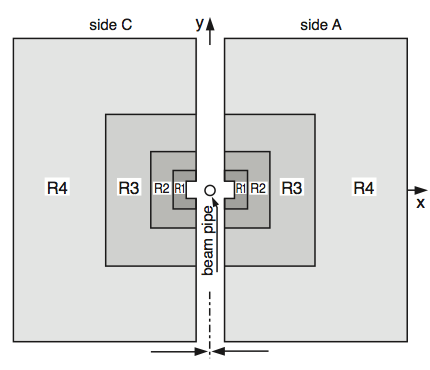
\includegraphics[width=\textwidth]{./Chapters/detector/muon_system/muon_regions.png}
			\caption{Front view of the muon station regions}
			\label{default}
		\end{subfigure}
	\end{center}
	\caption{Muon system layout}
	\label{fig: muon system layout}
\end{figure}

%\begin{table}[htdp]
%	\caption{Particles rates in the muon system, estimated in the Technical Design Report ~\cite{muon-tdr}}
%	\begin{center}
%		\begin{tabular}{|c|c|c|c|c|c|}
%			\hline
%			& M1 & M2 & M3 & M4 & M5 \\
%			\hline
%			R1 & 460 kHz & 37.5 kHz & 10 kHz & 6.5 kHz & 4.4 kHz \\
%			\hline
%			R2 & 186 kHz & 26.5 kHz & 3.3 kHz & 2.2 kHz & 1.8 kHz \\
%			\hline
%			R3 & 80 kHz & 6.5 kHz & 1 kHz & 0.75 kHz & 0.65 kHz \\
%			\hline
%			R4 & 25 kHz & 1.2 kHz & 0.42 kHz & 0.25 kHz & 0.23 kHz \\
%			\hline
%		\end{tabular}
%	\end{center}
%	\label{default}
%\end{table}%

The chambers are further subdivided into logical pads; the dimensions of which vary between muon stations. Stations M1-M3 are used in the muon trigger to calculate the $p_t$ of muon candidates (since muons are more attenuated at the further downstream muon stations) and so the granularity in the bending plane (horizontal) is finer than that of stations M4 and M5 (which are used to identify penetrating muons).

\begin{figure}[htbp]
	\begin{center}
			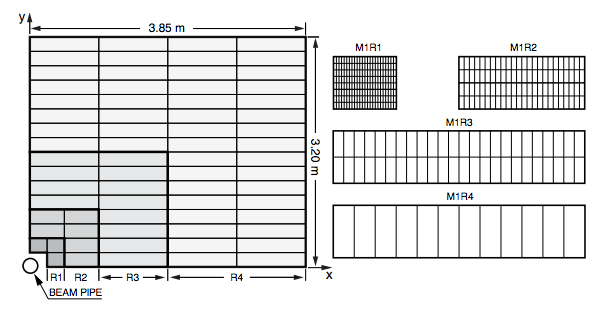
\includegraphics[width=\textwidth]{./Chapters/detector/muon_system/logical_pad_layout.png}
		\caption{On the left is a quadrant of the M1 station with the regions R1-R4 shown. Each rectangle represents a chamber. On the right are the chambers for regions, R1-R4 with the logical pad sub-structure shown}
		\label{fig: muon region granularity}
	\end{center}
\end{figure}

Overall the muon system has performed very well during the operation of LHCb achieving if not exceeding the requirements set by the Technical Design Report \cite{muon-tdr}. In particular efficiencies are well above the design requirements previously described \cite{Alves:2012ey}, see figure; efficiencies and mis Id rates together with the PID information from the RICH detector can be seen in figure \cite{Archilli:2013npa}. The momentum resolution achieved from the stand alone muon system reconstruction is ~25\% and ~0.4\% with the offline reconstruction using the tracking information \cite{Alves:2012ey}.























%\section{Particle Identification (PID)}
\section{Trigger}
\label{section: trigger}

\subsection*{Requirements}

The Large Hadron Collider was designed with a nominal bunch crossing rate of 40 MHz corresponding to a bunch crossing rate with at least one visible inelastic proton-proton interaction of $\sim$ 11 MHz \cite{Aaij:1493820}. The trigger system is required to select from these events rare interactions such as those involving the production of $\mathrm{b}\bar{\mathrm{b}}$ pairs, these events are typically characterised by the presence of particles with high transverse energy and momentum corresponding to daughter particles from the decay of the b quarks. To achieve this the trigger translates the raw detector hit information into physical processes and then decides on whether the event is to be kept. The time in which the trigger can achieve this is strictly constrained by the interaction rate in the LHCb detector. This rate is constantly being driven to higher values to get the most out of the detectors and maximise the data taking rate of experiments at the LHC. Such a dynamically changing environment requires an equally robust trigger.

\subsection*{Layout}

The trigger system is divided into two levels, the level 0 trigger (L0) and the High Level Trigger (HLT) \cite{Antunes-Nobrega:630828}. The high level trigger is further subdivided into two subsections, HLT1 and HLT2. For an event to pass the trigger it must pass each of the subdivisions in sequence (L0, HLT1, HLT2). Events selected by the trigger are then written to permanent data storage for further processing and analysis.

\subsubsection*{Level 0 Trigger (L0)}
The L0 trigger uses information from the muon and calorimeter systems. It identifies high transverse energy photons, hadrons and electrons from hits in the calorimeter system and high transverse energy muons from hits in the muon system. As the first level in the trigger system the L0 trigger makes more decisions that the following levels, to do this the trigger must be very fast. For this reason the decision algorithm is implemented in hardware with the electronics located inside the experiment and connected by optical fibres. The L0 trigger reduces the event rate from 40 MHz to 1.1 MHz with a maximum latency of $4\, \mu s$

\subsubsection*{High Level Trigger}
The high level trigger is a software implemented trigger system, it runs on the Event Filter Farm (EFF), a network of computers dedicated to making fast decisions about events \cite{1742-6596-396-1-012053}. The presence of a software based trigger in addition to the hardware based trigger increases the flexibility of the trigger system; providing a simple interface  to apply modification of parameters, implementation and computing resources without direct access to the physical components. 

The HLT has access to all the raw data from the LHCb detector, this event information is stored in raw banks e.g. energy clusters in the calorimeter system, hits in the tracking system. The HLT system uses a set of algorithms to decode the raw banks into event objects such as vertices, tracks and particles; this is known as the \emph{reconstruction} process. The event objects are passed as arguments to a decision algorithm which determines whether the event is kept depending on the properties of the event objects, e.g. a minimum transverse momentum requirement of particles produced in the event or a minimum impact parameter requirement between a particle and interaction vertex. For events which pass the event selection many of the event objects are stored to file in order to reduced the CPU processing requirements of its later analysis.

\subsubsection*{High Level Trigger 1 (HLT1)}
The HLT1 performs the initial reconstruction defining the vertices and tracks in the event. Its role in the trigger system has varied through the evolution of the experiment, displaying the versatility of the software trigger component of the trigger system. In the 2010 data taking period the role of the trigger was to confirm the decision of the L0 trigger matching the tracks made from the calorimeter and muon system to the VELO and TStation trackers together with other additional checks such as confirming the charge of particles detected at the L0 stage in order to minimise the misidentification of neutral particles. For the 2011 data taking period the HLT1 used a one track approach, basing the decision on the presence of at least one track passing a set of requirements such as, its impact parameter, transverse momentum, track fitting quality etc. For more information see. \cite{Antunes-Nobrega:630828} %edit

\subsubsection*{High Level Trigger 2 (HLT2)}
The HLT2 performs a higher level of reconstruction, matching track segments from each of the sub detector components to form a combined track with improved position and momentum resolution. Basic particle identification is applied these tracks to produce particle objects; this together with reconstruction of secondary vertices enable the reconstruction of both inclusive and exclusive decay channels e.g. $B \rightarrow hhhh$ or $B \rightarrow DX$. 

\subsection*{Offline Processing and Reprocessing}
Events which pass the trigger system are written to a permanent file storage system together with the full detector information. Before these data are made available for physics analysis there is an additional offline processing stage. In the offline environment the time requirements for processing each event are lessened allowing for more sophisticated algorithms to be run such as algorithms which decode particle identification information from the RICH system as well as advanced clone killing algorithms. 

Having the raw event information stored allows for reprocessing of the event information, this is useful since the reconstruction algorithms are constantly improving as well as the understanding of the detector and its alignment methods. Older data can then be reprocessed, giving event objects with greater resolution on their measurements i.e. are better representations of the corresponding physical particles.

\subsection*{Performance}

The trigger system has shown to be flexible and robust during the operation of the LHCb detector adapting to the larger pile-up conditions imposed by the machine delivering 1296 instead of the planned 2622 colliding bunches. The trigger rates of the LHCb detector in 2011 are outlined in table \ref{table: trigger performance} \cite{Aaij:1493820}.

\begin{table}[htdp]
	\caption{Trigger output rates during the 2011 data taking period}
	\begin{center}
		\begin{tabular}{|c|c|}
			\hline
			Trigger & Output Rate (kHz) \\
			\hline
			L0 & 870 \\
			HLT1 & 43 \\
			HLT2 & 3 \\
			\hline
		\end{tabular}
	\end{center}
	\label{table: trigger performance}
\end{table}%



\section{Computing}

The LHCb experiment provides an extremely challenging software environment. Requirements for such a software project include management of both large amounts of data as well as high rates of data; managing software written by a large number of collaborating scientists; managing frequent improvements and changes in algorithms; the ability to provide a common interface between generated data and measured data such that meaningful comparisons can be made; a constantly changing detector environment and the encapsulation of data relevant to a wide range of users.

The LHCb software is based on the Gaudi software architecture and framework \cite{Antunes-Nobrega:835156}. This framework is specifically design for use in the field of high energy physics and based on the concept of object orientated programming. Well defined interfaces are defined between components of the framework so that each component can be modified in a self contained manner without affecting other components. A schematic view of the Gaudi architecture is shown in figure \ref{fig: state of gaudi appliaction}, describing a typical state of the software model. 

\begin{figure}[h]
	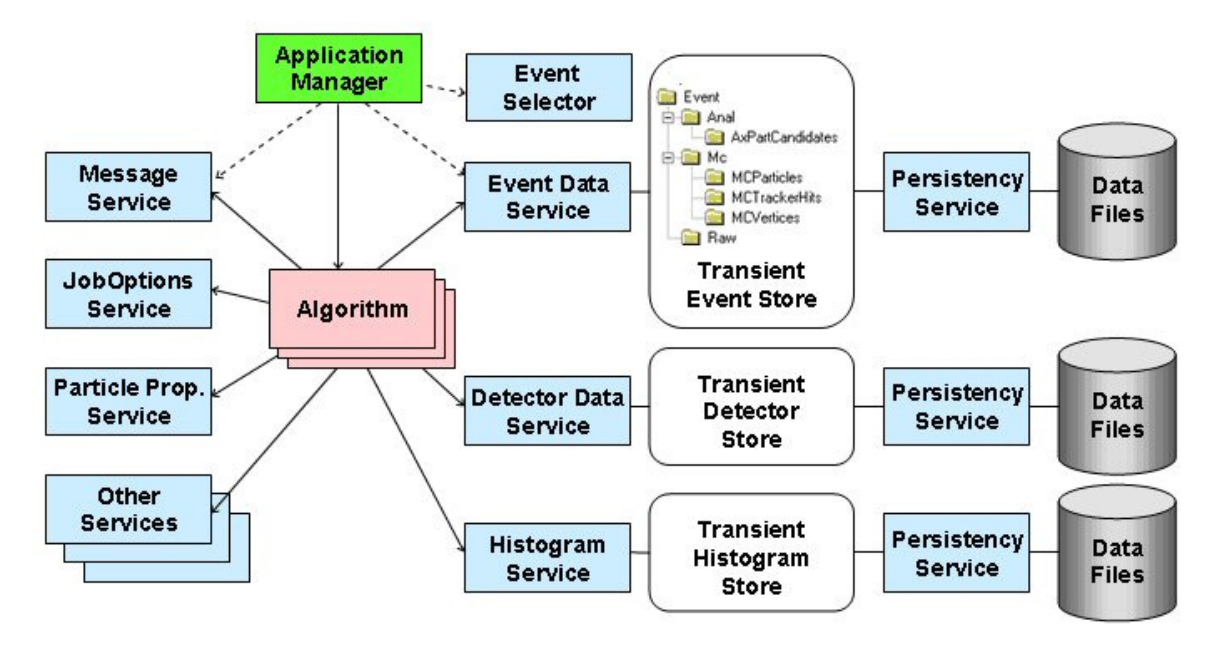
\includegraphics[width=\columnwidth]{/Users/admin/Dropbox/PhD/Thesis/Chapters/detector/computing/images/GaudiArchitecture.png}
	\caption{A state diagram of a typical application build on the Gaudi framework}
	\label{fig: state of gaudi appliaction}
\end{figure}

Unique to Gaudi architecture in comparison to other object orientated frameworks is the distinction between data and algorithms. In the Gaudi architecture algorithms themselves are objects and act on data objects (e.g. A track fitting algorithm acts on detector hit objects to form a track rather than the hits themselves forming a track). The motivation of this approach is shown in the persistency of algorithms and data objects. Algorithms are methods typically used to create objects such as tracks from detector hits; these methods are constantly being improved over the lifetime of the experiment. In contrast to this the models describing data are more stable (e.g. the concept of a track is not expected to change). Making a distinction between the algorithm and data decouples the two enabling the ability to modify the algorithms without affecting the data.

Each phase of the data processing is encapsulated into an application built on the Gaudi framework. Monte Carlo event generation and detector response to the generated particles is handled by the Gauss application, the output of this phase is in the form of detector hits and is used as input for the Boole application. The Boole application applies a detector response to the hits generated by the Gauss application digitising the hits into a format which mimics measured data. Additional hits are added from from Spillover events and LHC background and the digitisation step of the readout electronics, as well as of the L0 trigger hardware are simulated. The next phase of data processing is to reconstruct objects from the digitised hits, this is achieved through the Brunel application. Since the output from Boole is designed such that it models the detector output the algorithms used by Brunel are exactly the same for both generated data and data produced from measured collisions, decoupling the reconstruction phase completely from the generation phase. The output from the reconstruction phase is then proceeded by an analysis phase, the application for this phase is the DaVinci application. This phase is focused on the application of more sophisticated algorithms acting on high level objects such as particles and secondary vertices. This includes the reconstruction of exclusive decay channels and high level background correction. The overall application and data flow is outlined in figure \ref{fig: application data flow}.

\begin{figure}[h]
	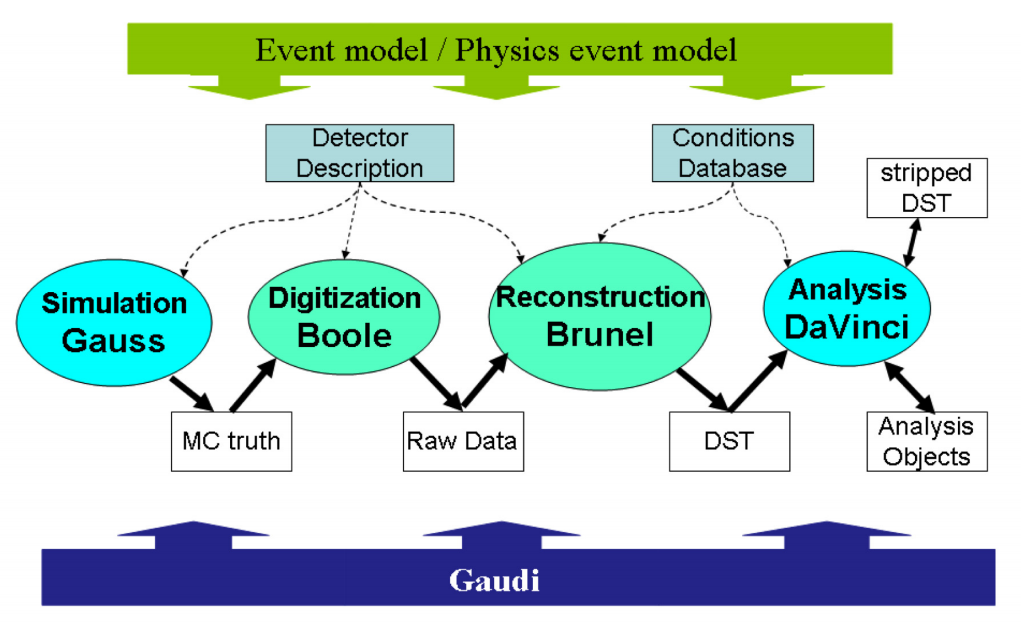
\includegraphics[width=\columnwidth]{/Users/admin/Dropbox/PhD/Thesis/Chapters/detector/computing/images/application_data_flow.png}
	\caption{A schematic of application processes and data flow. Underlying all the applications is the Gaudi framework. The arrows represent the transfer of input and output data.}
	\label{fig: application data flow}
\end{figure}

%In addition to the applications stated above there are many more applications focused on aspects of the operation of the LHCb detector e.g. online monitoring, interactive analysis and visualisation applications. For further information see \ref{}.

Information about the state of the LHCb detector at a given time is accessed via the Conditions Database service. This information includes such things as the temperature and pressure in certain detector elements as well as the alignment parameters used to describe the detector. The values stored in the database are dependent on several variables such as the time, version and data source of the data; each combination of variables is identified by a unique tag. Similarly information about the structure and materials of the detector elements are accessed via the Detector Descriptions Database and accessed via the Detector Description Service.

%The LHCb software is structured into several projects, each with a well defined functionality or application. Each project comprises of a set of packages. A package is defined as a set of files which together provide a well defined functionality. For example the Rec project contains packages related to the reconstruction process; these packages are organised such that they pertain to certain aspects of the reconstruction such as the tracking, calorimeters and particle identification. Dependencies between projects enable packages to be shared across projects, when building the software the dependencies are managed by the Configuration Management Tool (CMT).

To make use of the grid computing service the LHCb software uses the Distributed Infrastructure with Remote Agent's Control project (DIRAC). This together with the job submission application named Ganga, enables users to perform large scale physics analysis without having to the need for a complete understanding of the computing challenges behind their physics analyses.



	
%	\chapter{HPD image centre alignment}
\label{HPD image centre alignment}
\lhead{\emph{HPD image centre alignment}} % Write in your own chapter title to set the page header
%\section{Overview}
\section{Overview}

%1. What is an HPD
%2. What is its purpose
%3. Layout and dimensions
%4. Operation
%5. Performance
The Hybrid photon detectors (HPD) are used to detect Cherenkov photons emitted by particles traversing the RICH system. The hit positions of the emitted photons form a ring on the HPD plane, the radius of which is related to the Cherenkov angle associated to the particle. The Cherenkov angle of a particle acts as a signature of its particle type. This enables discrimination between electrons, pions, kaons and protons which is needed to identify the decay processes of particles produced in the LHCb detector. 

The HPDs are arrange in two grids, for RICH 1 [RICH 2] the grids are positioned above [left] and below [right] the beamline and are are arranged into rows of $14$ [$16$] by $7$ [$9$] columns (Fig \ref{fig: RICH 1: upper grid}). The HPDs are approximately cylindrical in shape, with a length of $160\,\mathrm{mm}$ and radius of $43.7\,\mathrm{mm}$ \footnote{There are small differences in the dimensions of the HPDs in RICH1 and RICH2. The values given here are for the HPDs in RICH 1, details for the HPDs in RICH 2 can be found in the RICH Technical design report.} (See Fig \ref{fig: HPD schematic} and Fig \ref{fig:HPD_photo}). A spherically-shaped cap quartz window is attached to one end of the HPD, on its inner surface is a deposition of an S20 (multi alkali) photo-cathode which emits photo-electrons when stimulated by photons. The emitted photo-electrons traverse the vacuum chamber of the HPD where they are accelerated by an electric potential difference of $20\,\mathrm{kV}$ onto a square silicon chip array of $32\,\times\,32$ pixels \footnote{When the HPD is run is its ALICE configuration the pixel dimensions are $32\,\times\,256$ pixels} with a length and width of $16\,\mathrm{mm}$.

\begin{figure}
	\begin{center}
		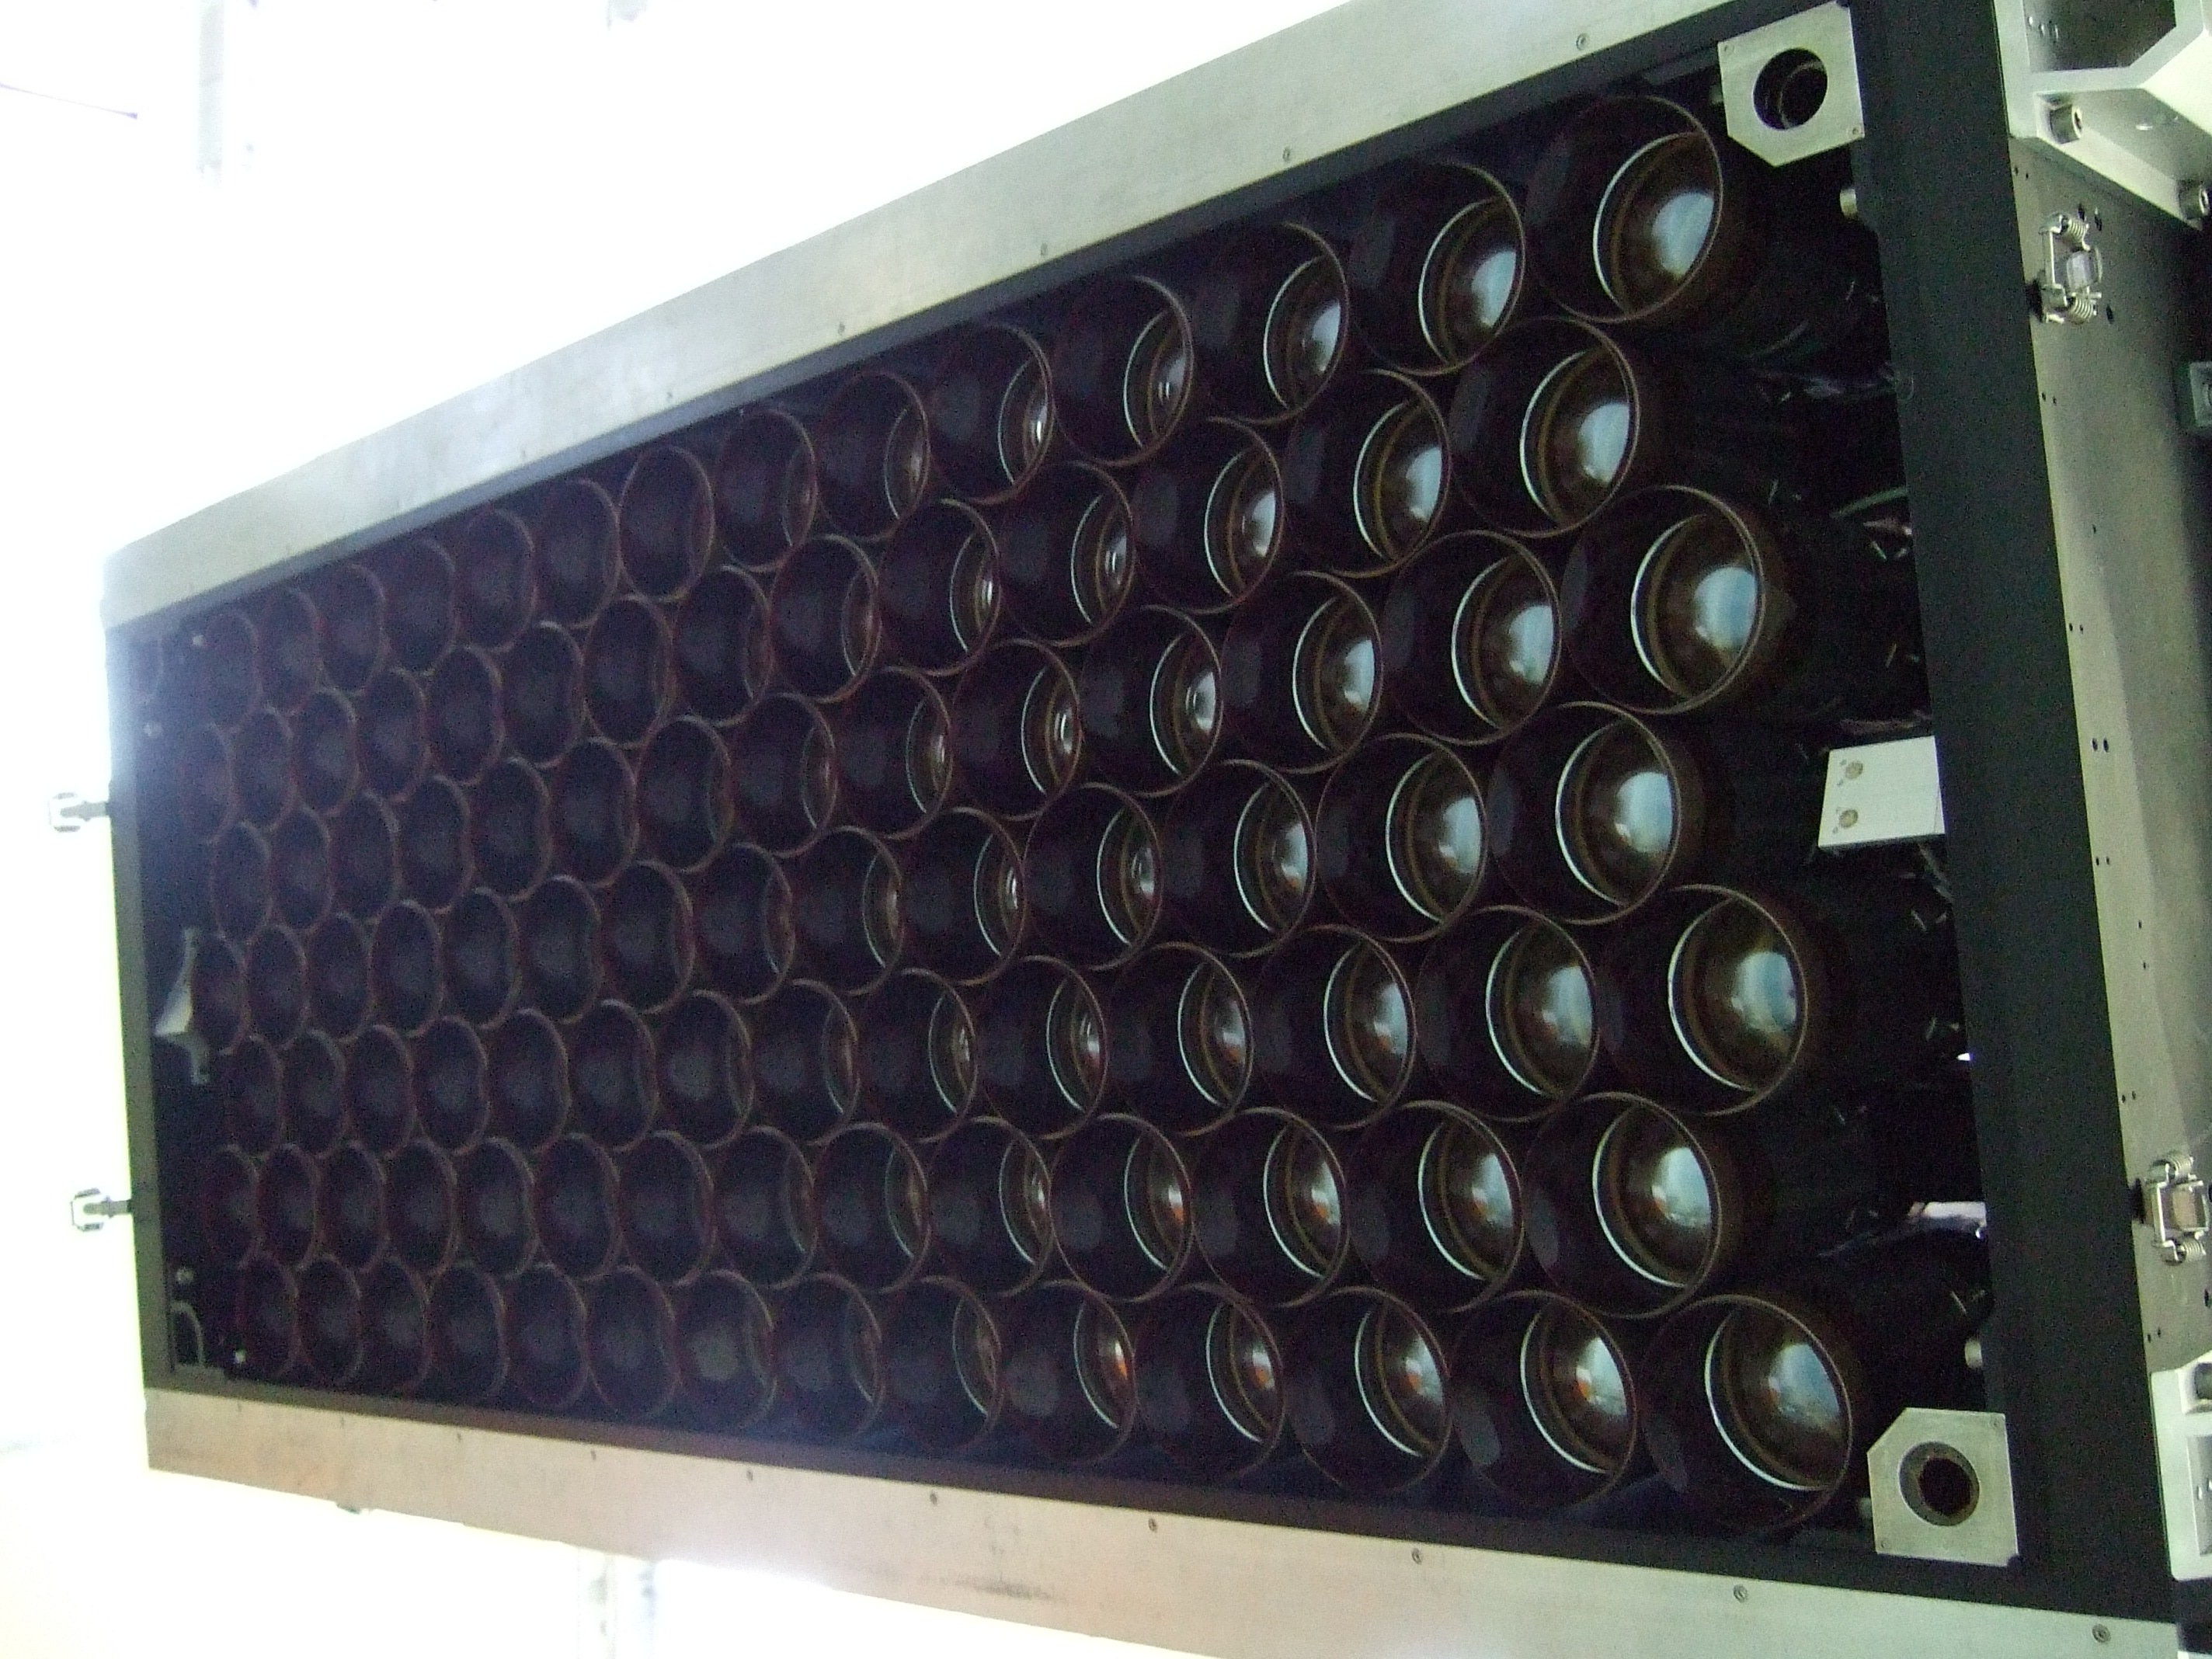
\includegraphics[width=0.5\columnwidth]{./Chapters/hpd_alignment/images/RICH1_Upper_box_134.jpg}
		\caption{Upper HPD grid in RICH 1}
		\label{fig: RICH 1: upper grid}
	\end{center}
\end{figure}

\begin{figure}
	\begin{minipage}[b]{0.45\linewidth}
		\centering
			\includegraphics[height=4cm, width=6cm]{$HOME/Dropbox/LHCb/detector/RICH/images/HPD_schematic2.png}
			\caption{HPD schematic}
			\label{fig: HPD schematic}
	\end{minipage}
	\hspace{0.5cm}
	\begin{minipage}[b]{0.45\linewidth}
		\centering
		\includegraphics[height=4cm]{$HOME/Dropbox/LHCb/detector/RICH/images/HPD_photo.jpg}
		\caption{photo of a HPD}
		\label{fig:HPD_photo}
	\end{minipage}
\end{figure}

The total accumulation of pixel signals over the course of a run can be visualised on a two dimensional plot called a hit map (or image summary fig \ref{example_HPD_image_summaries}). Due to the circular shape of the quartz window the hit map is circular in shape. An image centre is determined by fitting a circle to the boundary of the hit map and taking the central position. The accuracy in the position of the image centre is an important property of the HPD since any translation of the image centre affects the accuracy in the position of the photon, Cherenkov angle and particle identification. 

\begin{figure}
	\begin{center}
		\includegraphics[width=13cm]{$HOME/Dropbox/LHCb/detector/RICH/images/HPD_image_summaries.png}
		\caption{Example HPD hit maps for HPDs 001, 002 and 092 for run 80168. The z-axis corresponds to the number of hits registered by a pixel, the x and y axes correspond to the pixel position on the silicon chip}
		% comment: Either change the naming convention of the HPDs to match U half / D half notation and include image of layout of include image of numbered naming convention
		\label{example_HPD_image_summaries}
	\end{center}
\end{figure}

Observations of the image centre show that its position does not necessarily line up with the centre of the silicon chip, this effect is accounted for by an alignment process which reflects the displacement of the image centre from the silicon chip centre in the detector description of the LHCb detector. In addition, during the course of operation, shifts in the position of the image centre for individual HPDs have been consistently observed. These shifts can be as much as $2\,\mathrm{mm}$ (Fig \ref{fig: shift_distance}) between consecutive runs. This phenomenon was further confirmed during and investigation carried out in laboratory tests performed at the end of 2009 using HPDs removed from the LHCb detector for which shifts has been most noticeably observed. The low levels of mechanical stress, scale of the shifts (Fig \ref{fig: 2010 displacement}) and rigidity of the HPD fixings suggest the image shifts are not due to physical movement of the HPD components, but are instead the result of disturbances to the electric fields due to build up of charge on HPD components over the duration of operation. Additionally shifts were shown to be present across both magnetic field configurations and when the magnet was off suggesting this effect was not an artefact of the magnet.

In addition to the alignment of the HPD image centres the performance of the RICH detector is also dependent on the alignment of its other components. In particular the alignment of the mirrors which reflect the Cherenkov radiation onto the HPD plane and the Magnetic distortion monitoring system (MDCS) which corrects distortion effects to the HPDs due to the magnetic field from the LHCb magnet. These alignment procedures are intimately entangled such that changes in any of the alignment procedures will affect the other. Since improvements in the individual alignment systems are constantly ongoing in parallel it can be difficult to disentangle how the effect of changes in the individual alignment systems affects the RICH system as a whole. 

The work presented here builds on alignment techniques performed previously for the data collected in 2010. The main changes were to carry out the alignment on a run by run basis. For the data taking period of 2010 the HPD image centres were calculated by averaging over the whole year. Improvements were also made to the general stability and accuracy of the fit. At the time of writing the current alignment software produces improvements $\sim7\%$ in RICH1 and RICH2 (section \ref{chap: application of correction factors}) compared to the 2010 alignment techniques.

\begin{figure}
	\begin{center}
		\caption{Image centre x,y displacement and shifts for 2010 tagged consecutive runs ranging from 68179 - 80168}
		\label{fig: 2010 displacement}
		\begin{subfigure}[b]{\textwidth}%[x-displacement]
		{
			\begin{center}
				\includegraphics[width=.6\columnwidth]{/afs/cern.ch/user/d/dvoong/analysis/rich/HPDs/image_fitting/displacement_between_conseq_runs/scripts/x_displacement.png}
			\end{center}
			\caption{Displacement in x}
			\label{fig: x_displacement}
		}
		\end{subfigure}
		\begin{subfigure}[b]{\textwidth}
		{	
			\begin{center}
				\includegraphics[width=.6\columnwidth]{/afs/cern.ch/user/d/dvoong/analysis/rich/HPDs/image_fitting/displacement_between_conseq_runs/scripts/y_displacement.png}
			\end{center}
			\caption{Displacement in y}
			\label{fig: y_displacement}
		}
		\end{subfigure}
		\begin{subfigure}[b]{\textwidth}
		{
			\begin{center}
				\includegraphics[width=.6\columnwidth]{/afs/cern.ch/user/d/dvoong/analysis/rich/HPDs/image_fitting/displacement_between_conseq_runs/scripts/shift_distance.png}
			\end{center}
			\caption{Distance}
			\label{fig: shift_distance}
		}
		\end{subfigure}
	\end{center}
\end{figure}

The shifting of images was first noticed in the middle of 2009 most noticeably in a HPD located around the outer corner (HPD: A7 13) of the the A-side HPD plane (Fig \ref{fig: RICH2_HPD_plane_layout}). The RICH2 HPD intervention in October 2009 was used as an opportunity to extract the HPD to investigate image shifts in a laboratory environment. 

The set up for the laboratory tests were chosen so that the conditions were as similar as possible to the conditions in the LHCb detector. Tests were performed over time periods varying from 48 to 450 hours using an LED light source. Figure \ref{fig: november lab test} shows the results from a 48 hour period test, Figure \ref{fig: thierry row} [\ref{fig: thierry col}] shows the variation in the row [column] position of the image centre and figure \ref{fig: thierry radius} shows the variation in the radius of the circle used to fit the HPD hit map. In January 2010 the tests were repeated over a 450 hour period to investigate whether the shifts exhibited oscillatory behaviour, results are shown in figure \ref{fig: january lab test}, no significant repeating behaviour was observed.

\begin{figure}
	\begin{subfigure}[b]{\textwidth}
		\begin{center}
			\includegraphics[width=0.7\columnwidth]{$HOME/Dropbox/LHCb/detector/RICH/HPDs/alignment/thierry_stuff/november_lab_tests/pngs/row_position.png}
			\caption{image centre row position, note: lab test were performed with HPD in Alice mode meaning a greater number of effective pixels on the chip (8 Alice pixels to 1 LHCb pixel (0.5mm))}
			\label{fig: thierry row}
		\end{center}
	\end{subfigure}
	\begin{subfigure}[b]{\textwidth}
	{
		\begin{center}
			\includegraphics[width=0.7\columnwidth]{$HOME/Dropbox/LHCb/detector/RICH/HPDs/alignment/thierry_stuff/november_lab_tests/pngs/column_position.png}
			\caption{image centre column position}
			\label{fig: thierry col}
		\end{center}
	}
	\end{subfigure}
	\begin{subfigure}[b]{\textwidth}
	{
		\begin{center}
			\includegraphics[width=0.7\columnwidth]{$HOME/Dropbox/LHCb/detector/RICH/HPDs/alignment/thierry_stuff/november_lab_tests/pngs/radius.png}
			\caption{image radius}
			\label{fig: thierry radius}
		\end{center}
	}
	\end{subfigure}
	\caption{HPD A7 13 image shift lab test results over a period of four days}
	\label{fig: november lab test}
\end{figure}

\begin{figure}
	\includegraphics[width=\columnwidth]{$HOME/Dropbox/PhD/service_work/HPD_alignment/internal_note/images/january_lab_test.png}
	\caption{HPD image centre shift laboratory tests in January 2010. HPDs image shifts were monitored over a 450 hour period}
	\label{fig: january lab test}
\end{figure}

%%%%%%%%%%%%%%%%%%%%%%%%%%%%%%%%%%%%%%%%%%%%%%%%%%%%%%%%%%%%%%%%%%%%%%%%
%                                                                                   		IMAGE FITTING TECHNIQUE											        %
%%%%%%%%%%%%%%%%%%%%%%%%%%%%%%%%%%%%%%%%%%%%%%%%%%%%%%%%%%%%%%%%%%%%%%%%
\section{Image fitting technique}
\label{section: Fitting Procedure}

Image fitting is applied to the accumulated hit maps in order to find the centre of the image. A boundary finding procedure is first employed to find the edges of the images, once the boundary is determined a $\chi^2$ minimisation is performed to fit a circle to the boundary. Various boundary finding methods were investigated, two of these are outline below, 1. Threshold boundary fitting and 2. Sobel boundary fitting.

%Shifts in the image centre translate to a shift in the effective position of the silicon chip sensor. From this it follows that if this shift is not corrected for then some error will be associated to projection of photons on the HPD hence their Cherenkov angles. This is corrected by modifying the LHCb detector database to include information on the HPD image centre positions (translated to the silicon chip position). Since the image centre positions vary with time it is necessary to to split the database up into slices such that each slice corresponds to a run period.

%The alignment procedure involves fitting the HPD hit map (fig \ref{example_HPD_image_summaries}), this involves first marking out a boundary to the image which is then fitted with a circle from which the centre is taken as the image centre. %, this is followed by a correction to the image centre to compensate for the displacement from its nominal position. This steps of this process are outlined below,

%\begin{enumerate}
%	\item Calculate an image boundary for the hit map
%	\item Fit a circle to the image boundary and take the centre of the circle as the centre of the hit map
%	\item Record image centre in the LHCb conditions database with a timestamp corresponding to the time of the run
%	\item Rerun the reconstruction software with the updated conditions database for the end of year reprocessing (Since the hit map is produced from data collected over the total duration of a run it is not possible to perform an online alignment at the time of data taking)
%\end{enumerate}

%A private database together with a full RICH reconstruction was carried out to test the effect of the alignment procedure on the Cherenkov angle resolution.

%%%%%%%%%%%%%%%%%%%%%%%%%%%%%%%%%%%%%%%%%%%%%%%%%%%%%%%%%%%%%%%%%%%%%%%%
%                                                                                   		BOUNDARY SELECTION PROCEDURE									        %
%%%%%%%%%%%%%%%%%%%%%%%%%%%%%%%%%%%%%%%%%%%%%%%%%%%%%%%%%%%%%%%%%%%%%%%%
\subsection {Boundary selection procedure}
The boundary selection method uses an iterative algorithm to scan over the hit map scanning from the pixels in the outer region towards the centre. A test is applied to each pixel with a set of criteria to meet, the outermost pixels which pass the test are then marked as part of the boundary of the image. The Sobel boundary fitting method incorporates an additional process applied to the hit map prior to the boundary selection, this process emphasises regions in the image with large changes to the image intensity hence emphasising the image boundaries.


%The alignment software provides two different methods for fitting the image centre of a HPD hit map. These correspond to the two different methods for fitting the boundary (the circle fitting procedure for the two methods is the same). The two boundary fitting methods are outlined in the following sections.

%The boundary of the image can be calculated by two possible methods which are outlined in the following sections. In general the boundary selection method uses an iterative algorithm to scan over the hit map scanning from the pixels in the outer region towards the centre. A test is applied to each pixel with a set of criteria to meet, the outermost pixels which pass the test are marked as part of the boundary of the image. 

%, the criteria are as follows,
%The boundary of the image can be calculated by two possible methods, these are outlined in the following sections.
%The algorithm can be configured to scan the image in various orders, e.g. columns followed by rows and vice-versa.


%%%%%%%%%%%%%%%%%%%%%%%%%%%%%%%%%%%%%%%%%%%%%%%%%%%%%%%%%%%%%%%%%%%%%%%%
%                                                                                   		THRESHOLD BOUNDARY FITTING										        %
%%%%%%%%%%%%%%%%%%%%%%%%%%%%%%%%%%%%%%%%%%%%%%%%%%%%%%%%%%%%%%%%%%%%%%%%
\subsubsection{Threshold boundary fitting}

The threshold boundary method uses two criteria to determine the boundary pixels.

\begin{description}
	\item[Criteria 1] \hfill \\ The number of hits for a pixel must pass a user defined threshold parameter. The parameter is defined such that a value of 1 corresponds to the average number of hits per pixel for the HPD image. The optimal threshold value is calculated by comparing the Cherenkov angle resolution as a function of the threshold value.
	\item[Criteria 2] \hfill \\ At least one of its adjacent pixels must also pass requirement 1, this requirement reduces the contribution of pixels with unexpectedly high population (noisy pixels). This can occur when there is a fault with an individual pixel.
\end{description}

%The threshold boundary fitting method carries on from the 2010 alignment software approach, the simpler of the two methods, it involves an iterative algorithm which effectively scans over the pixel map on the silicon chip scanning from the outer regions of the chip to the centre. The first pixel to satisfy the following requirements marks the a boundary point on the HPD image summary,

%The threshold boundary method uses an iterative algorithm to scan over the hit map scanning from the pixels in the outer region towards the centre. A test is applied to each pixel with a set of criteria to meet, the outermost pixels which pass the test are marked as part of the boundary of the image, the criteria are as follows, 

%comment: Need some plots of boundary selection using threshold method
%In the 2010 software the boundary algorithm scanned {\bf only} the from top to bottom and from bottom to top of the HPD. The 2011 software additional scans horizontally and determines a boundary from the convolution of both directions. The differences can be seen in figure \ref{fig: comparison of 2010, 2011 boundary fitting}
%Needs more detail of what I'm looking at in the Figure.
%\begin{figure}[ht]
%	\begin{center}
%	\subfloat[2010]
%	{
%		\includegraphics[height = 4cm, width = 4cm]{/Users/admin/Pictures/scruffy_dog_small.jpg}
%		\label{fig:simple boundary fitting 2010}
%	}
%	\subfloat[2011]
%	{
%		\includegraphics[height = 4cm, width = 4cm]{/Users/admin/Pictures/scruffy_dog_small.jpg}
%		\label{fig:simple boundary fitting 2011}
%	}
%	\caption{Comparison of simple boundary fitting 2010 and 2011} 
%	\label{fig: simple boundary fitting comparison}
%	\end{center}
%\end{figure}

%\begin{figure}
%\begin{center}
%\includegraphics[width=13cm]{$HOME/Dropbox/LHCb/detector/RICH/images/boundary_fitting_comparison.pdf}
%\caption{Boundary fitting comparison: left) 2010, centre) HPD image summary with image cleaning and Sobel filter applied, right) HPD image summary with fitted circle of centre image overlaid}
%\label{fig: comparison of 2010, 2011 boundary fitting}
%\end{center}
%\end{figure}

% Put image of 2010 boundary fitting here too

%\begin{figure}
%\begin{center}
%\includegraphics[width=13cm]{$HOME/Dropbox/LHCb/detector/RICH/images/HPD_image_summaries_boundary.png}
%\caption{HPD image summaries from figure \ref{example_HPD_image_summaries} with boundaries fitted using the 2011 simple boundary fitting method}
%\label{fig: simple boundary fitting 2011}
%\end{center}
%\end{figure}

% figures showing the boundary fitting algorithm for 2010 and 2011


%%%%%%%%%%%%%%%%%%%%%%%%%%%%%%%%%%%%%%%%%%%%%%%%%%%%%%%%%%%%%%%%%%%%%%%%
%                                                                                   		SOBEL BOUNDARY FITTING										        	        %
%%%%%%%%%%%%%%%%%%%%%%%%%%%%%%%%%%%%%%%%%%%%%%%%%%%%%%%%%%%%%%%%%%%%%%%%
\subsubsection{Sobel boundary fitting}


Similarly to the threshold boundary method the Sobel method also uses a set of criteria to select a boundary, however, before this process a filter is applied to the HPD hit image which maps the intensity ($I$) of a pixel to its intensity gradient in relation to its adjacent pixels. An example of the Sobel filter being used in the field of image processing can be seen in figure \ref{fig: sobel example} and an example of the application of the Sobel filter to a HPD image is shown in figure \ref{fig: HPD image with Sobel filter applied}. The intensity gradient is calculated by calculating the horizontal and vertical intensity gradients for a pixel and combining them using Pythagoras theorem,

\begin{equation}
	\frac{\partial I}{\partial \vec{r}} \approx \sqrt{\left(\frac{\partial I}{\partial x}\right)^2 + \left(\frac{\partial I}{\partial y}\right)^2}
\end{equation}

For a pixel located on row $i$ and column $j$ the horizontal intensity gradient is given by, 

\begin{equation}
	\left(\frac{\partial I}{\partial x}\right)_{(i,j)} = (I_{(i+1,j-1)} - I_{(i+1, j+1)}) + 2(I_{(i,j-1)} - I_{(i, j+1)}) + (I_{(i-1,j-1)} - I_{(i-1, j+1)})
\end{equation}

where the first term is equal to the difference between the lower diagonal left and lower diagonal right pixels; the second term is the difference between the left and right pixels weighted by a factor of two; the third term is the difference between the upper diagonal left and upper diagonal right pixels. Similarly for the the vertical intensity gradient,

\begin{equation}
	\left(\frac{\partial I}{\partial y}\right)_{(i,j)} = (I_{(i-1,j+1)} - I_{(i+1, j+1)}) + 2(I_{(i-1,j)} - I_{(i+1, j)}) + (I_{(i-1,j-1)} - I_{(i+1, j-1)})
\end{equation}

where the first term is difference between the lower diagonal left and upper diagonal left pixels; the second term is difference between the lower and upper pixels weighted by a factor of two; the third term is difference between the lower diagonal right and upper diagonal right pixels.

A boundary finding algorithm is then applied to the filtered hit map, the boundary pixels are required to match the following criteria,

\begin{description}
	\item[Criteria 1] \hfill \\ The intensity gradient of a pixel must pass a user defined threshold parameter. The optimal threshold value is calculated by comparing the Cherenkov angle resolution as a function of the threshold value.
	\item[Criteria 2]\hfill \\ The pixel must be either a peak pixel (adjacent pixels on the same column or row must have a lower intensity gradient) or be adjacent to a peak pixel and have an intensity gradient greater than a user defined threshold value that is related to the intensity gradient of its corresponding peak pixel.
\end{description}

An example of the boundary finding algorithm can be seen in figure \ref{fig: comparison of 2010, 2011 boundary fitting}.

\begin{figure}[h]
	\begin{center}
		\includegraphics[width=13cm]{$HOME/Dropbox/LHCb/detector/RICH/images/sobel_example.png}
		\caption{An example of the Sobel filter in action}
		\label{fig: sobel example}
	\end{center}
\end{figure}

\begin{figure}[h]
	\begin{center}
		\includegraphics[width=13cm]{$HOME/Dropbox/LHCb/detector/RICH/images/Sobel_filtered_image.png}
		\caption{HPD image summary with Sobel filter applied}
		\label{fig: HPD image with Sobel filter applied}
	\end{center}
\end{figure}

%This can be visualised as 
%
%In the case of the horizontal intensity gradient this  taking the difference between intensities of adjacent pixels on the left and right columns and summing this with the difference between the intensities of the diagonally left and right pixels for the above and below rows. In addition the pixels on the central row contribute more to the intensity gradient and are given a weight of twice that for the diagonals. The weighting for the horizontal intensity gradient is visualised below, \\

%Qualitatively this is equivalent to, in the case of the horizontal intensity gradient, taking the difference between intensities of adjacent pixels on the left and right and summing this with the difference between the intensities of the diagonally left and right pixels for the above and below rows. In addition the pixels on the central row contribute more to the intensity gradient and are given a weight of twice that for the diagonals. The weighting for the horizontal intensity gradient is visualised below, \\

%\begin{center}
%$
%	\left( \begin{array}{ccc}
%	-1 & 0 & 1 \\
%	-2 & 0 & 2 \\
%	-1 & 0 & 1 \end{array} \right)
%$
%\end{center}
%
%Similarly in the case of the vertical intensity gradient, the intensity gradient is given by the difference between intensities of adjacent pixels on the top and bottom and summing this with the difference between the intensities of the diagonally top and bottom pixels for the left and right columns. Again the weighting is different for each column.
%
%\begin{center}
%$
%	\left( \begin{array}{ccc}
%	-1 & -2 & -1 \\
%	 0 &  0  &  0  \\
%	 1 &  2  &  1 \end{array} \right)
%$
%\end{center}

%Again what I'm I looking at Fig 2.3
%The Sobel method is the default method for boundary fitting, it has been shown to significant improve on the threshold boundary method. The Sobel method involves first applying the Sobel operator to the hit map. For a generic image the application of the Sobel operator produces a map of image intensity gradients (fig \ref{sobel example}). In the case of the HPD image this corresponds to the variation in the intensity of hits on the pixels on the silicon chip. The result of this can be seen in fig \ref{fig: HPD image with Sobel filter applied}. The peak regions in the image intensity gradient map correspond to the boundary region of the unprocessed image, the problem of finding the boundary of the unprocessed image is then simplified to finding the peak regions in image gradient map.

%%%

%\subsection{The Sobel operator}
%\label{sec: the Sobel operator}
%The Sobel operator is a discrete differentiation operator, computing an approximation of the gradient of the image intensity function.
%Defining A as the image source, $*$ is the convolution operator and $G_x$, $G_y$ as the respective gradients of the image we have,
%\begin{center}
% \[
% G_x =  
%\left( \begin{array}{ccc}
%-1 & 0 & 1 \\
%-2 & 0 & 2 \\
%-1 & 0 & 1 \end{array} \right) * A 
%\]
%\[ 
%G_y =  
%\left( \begin{array}{ccc}
%-1 & -2 & -1 \\
%0 & 0 & 0 \\
%1 & 2 & 1 \end{array} \right) * A 
%\]  \\
%\[
%G = \sqrt{G_x^2 + G_y^2} 
%\] \newline
%
%\end{center}
%
%In the case of the vertical operator the operation on a pixel at $(x_1, y_1)$  calculates the intensity difference between the above and below pixels weighted by two summed with the intensity difference of the above right and below right pixels and of the top left and bottom left pixel both weighted by a factor of 1. \newline
%
%\begin{table}[htdp]
%\begin{center}
%\begin{tabular}{|c|c|c|}
%\hline
%{\cellcolor[gray]{0.8}} & {\cellcolor[gray]{0.}} & {\cellcolor[gray]{0.8}} \\ 
%\hline
% &  &  \\ 
%\hline
%{\cellcolor[gray]{0.8}} & {\cellcolor[gray]{0}} & {\cellcolor[gray]{0.8}} \\
%\hline
%\end{tabular}
%\caption{the vertical intensity gradient of the centre pixel is calculated by summing the difference between the respective pixels in the above and below rows. The black pixels are weighted by a factor of 2 and the grey are weighted by a factor of 1}
%\end{center}
%\end{table}%
%
%$dI(x_1, y_1)/dy \approx 2\times \{I(x_1, y_1+1) - I(x_1, y_1-1)\} + \{I(x_1+1, y_1+1) - I(x_1+1, y_1-1)\} + \{I(x_1-1, y_1+1) - I(x_1+1, y_1-1)\} $

%%%

%alternatively, relative to a non-edge pixel with image intensity $I$, \newline
%\begin{center}
%
%$\frac{\partial I(n,m)}{\partial x} \approx I(n+1, m+1) - I(n+1, m-1) + 2*(I(n, m+1)-I(n, m-1)) + I(n-1, m+1) - I(n-1, m-1)$ \newline
%
%$\frac{\partial I(n,m)}{\partial y} \approx I(n-1, m-1) - I(n+1, m-1) + 2*(I(n-1, m)-I(n+1, m)) + I(n-1, m+1) - I(n+1, m+1)$ \newline
%
%$\frac{\partial I(n,m)}{\partial r} \approx \sqrt{\frac{\partial I(n,m)}{\partial x}^2 + \frac{\partial I(n,m)}{\partial y}^2}$ \newline

%$\frac{\partial I}{\partial x} \approx I_{top\,right} - I_{top\,left} + 2*(I_{right} - I_{left}) + I_{bottom\,right} - I_{bottom\,left} $ \newline
%
%$\frac{\partial I}{\partial y} \approx I_{bottom,left} - I_{top\,left} + 2*(I_{bottom} - I_{top}) + I_{bottom\,right} - I_{top\,right}$ \newline
%
%\[
%\frac{\partial I}{\partial r} \approx \sqrt{\frac{\partial I}{\partial x}^2 + \frac{\partial I}{\partial y}^2}
%\]
%
%$r = \sqrt{x^2 + y^2}$

%\end{center}

%A lot more detail needed in this section outlining the method. As a non-expert I'm afraid I'm non the wiser of what's going on having read the section


 
 %%%%%
 
 \newpage
 
%%%%%%%%%%%%%%%%%%%%%%%%%%%%%%%%%%%%%%%%%%%%%%%%%%%%%%%%%%%%%%%%%%%%%%%%
%                                                                                   		CIRCLE FITTING										        	        		        %
%%%%%%%%%%%%%%%%%%%%%%%%%%%%%%%%%%%%%%%%%%%%%%%%%%%%%%%%%%%%%%%%%%%%%%%%
\subsection{Circle fitting}
The circle fitting procedure is carried out by minimising the chi squared function,
\begin{equation}
 \chi^2(x_0, y_0, r) = \sum \limits_{n=0}^{N}\left(\sqrt{(x_n-x_0)^2 + (y_n-y_0)^2} - r\right)^2 \cdot I_n
\end{equation}
where $x_0$ and $y_0$ correspond to the x and y coordinates of the centre of the circle, $r$ the radius and $(x_n, y_n, I_n)$ are the $x$, $y$ coordinates and intensity for the boundary pixel $n$. Results for the image centre fitting using both the threshold and Sobel boundary finding techniques are shown in figure \ref{fig: comparison of 2010, 2011 boundary fitting}.

\begin{figure}
	\begin{center}
		\includegraphics[width=13cm]{$HOME/Dropbox/LHCb/detector/RICH/images/boundary_fitting_comparison.pdf}
		\caption{Boundary fitting comparison: left) 2010, centre) HPD image summary with image cleaning and Sobel filter applied, right) HPD image summary with fitted circle of centre image overlaid}
		\label{fig: comparison of 2010, 2011 boundary fitting}
	\end{center}
\end{figure}

%Why's this factor of 12 here? It's a constant and won't affect the chi-squared minimisation

 %%%%%

%\subsection{Additional changes to the 2010 fitting code}

%%%%%%%%%%%%%%%%%%%%%%%%%%%%%%%%%%%%%%%%%%%%%%%%%%%%%%%%%%%%%%%%%%%%%%%%
%                                                                                   	ADDITIONAL IMAGE STABILISATION										        %
%%%%%%%%%%%%%%%%%%%%%%%%%%%%%%%%%%%%%%%%%%%%%%%%%%%%%%%%%%%%%%%%%%%%%%%%
\subsection{Additional Image Stabilisation} 

Defects in individual HPDs can result in undesirable effects in the detection of particles from proton-proton interactions in the LHCb detector. For example, a defective pixel may exhibit a high population of hits which do not correspond to any physics event. These are referred to as hot pixels. Similarly a defective pixels might not detect any signal at all, these are known as dead pixels. To minimise the the effect of these hot/dead pixels on the HPD image centre calculations smoothing is applied to suspected defective pixels (see figures \ref{image cleaning: hot pixel} and \ref{image cleaning: dead column}). 

Hot pixels are determined by comparing the population of a pixel to the average population for a pixel calculated as the sum of pixel hits divided by the total number of pixels. A conservative threshold value is chosen and the central region is not scanned to ensure only defective pixels are selected. Dead pixels are selected from pixels that have no hits but have neighbouring pixels with a population greater than a user defined threshold value. Again a conservative threshold is chosen to ensure only defective pixels are selected.

\begin{figure}
	\begin{subfigure}[b]{0.45\textwidth}
		\includegraphics[width=\textwidth]{$HOME/Dropbox/LHCb/detector/RICH/images/image_cleaning_hot_pixel.png}
		\caption{Image cleaning: hot pixel example}	
		\label{image cleaning: hot pixel}
	\end{subfigure}
	\begin{subfigure}[b]{0.45\textwidth}
		\includegraphics[width=\textwidth]{$HOME/Dropbox/LHCb/detector/RICH/images/image_cleaning_dead_column.png}
		\caption{image cleaning: dead column example}
		\label{image cleaning: dead column}	
	\end{subfigure}
	\caption[Optional caption for list of figures]{Other changes to the 2010 fitting code}	
	\label{fig: Other changes to the 2010 fitting code}
\end{figure}

%\begin{figure}[ht]
%	\subfloat[Image cleaning: hot pixel example]
%	{
%		\includegraphics[width=13cm]{$HOME/Dropbox/LHCb/detector/RICH/images/image_cleaning_hot_pixel.png}
%		\label{image cleaning: hot pixel}
%	}
%	\\
%	\subfloat[image cleaning: dead column example]
%	{
%		\includegraphics[width=13cm]{$HOME/Dropbox/LHCb/detector/RICH/images/image_cleaning_dead_column.png}
%		\label{image cleaning: dead column}
%	}
%	\label{fig: Other changes to the 2010 fitting code}
%	\caption[Optional caption for list of figures]{Other changes to the 2010 fitting code}
%\end{figure}


%%%%%%%%%%%%%%%%%%%%%%%%%%%%%%%%%%%%%%%%%%%%%%%%%%%%%%%%%%%%%%%%%%%%%%%%%
%                                                                                   CHERENKOV RADIATION										        	        %
%%%%%%%%%%%%%%%%%%%%%%%%%%%%%%%%%%%%%%%%%%%%%%%%%%%%%%%%%%%%%%%%%%%%%%%%
\section{Cherenkov Radiation}

Charged particles traversing through a medium at a speed greater than the speed of light in the same medium emit electromagnetic radiation known as Cherenkov radiation. The angle at which the radiation is emitted relative to the direction of the particle (Cherenkov angle) is constant given the speed of the particle and the refractive index of the medium are also constant. The relationship between the speed of the particle ($\beta = \frac{|\vec{v}|}{c}$), refractive index of the medium ($n$) and the Cherenkov angle ($\theta_C$) is described by the equation,

\begin{equation}
	\cos{\theta_C} = \frac{1}{n\beta}\\
	\label{equation: Cherenkov radiation}
\end{equation}

The speed of the particle, $\beta$ can be expressed in terms of its mass $m$ and momentum $\vec{p}$,

\begin{eqnarray}
	\beta&=&\frac{|\vec{p}|}{E}
	= \frac{|\vec{p}|}{\sqrt{\vec{p}^2 + m^2}}
	= \frac{1}{\sqrt{1 + \frac{m^2}{\vec{p}^2}}}
%	= \frac{\gamma m |\vec{v}|}{\gamma m} \,\,\,\,\,\,\,\,\,\,\,\,\,\,\,\,\,\,\,\, c = 1
\end{eqnarray}

The equation for the Cherenkov angle can then be expressed in terms of mass and momentum,

\begin{equation}
	\cos{\theta_C} = \frac{1}{n}\sqrt{1 + \frac{m^2}{\vec{p}^2}}
	\label{equation: Cherenkov angle in terms of mass and momentum}
\end{equation}

In this form the particle type of a particle can be determined from knowledge its momentum and the corresponding angle of Cherenkov radiation produced by it. 

For a medium with refractive index $n$ and where $|\vec{p}| >> m$ the Cherenkov angle becomes \emph{saturated} such that for all particle types the Cherenkov equation can be expressed as,

\begin{equation}
	\cos{\theta_C^{max}} = \frac{1}{n}
	\label{equation: saturated Cherenkov radiation}
\end{equation}

\begin{equation}
	\theta_C^{max}(\pi) = \theta_C^{max}(K) = \theta_C^{max}(p)
\end{equation}

Saturation of the Cherenkov angle in the LHCb RICH detector can be seen in figure \ref{fig: RICH radiator}.

\begin{figure}[h]
	\begin{center}
		\includegraphics[width=8.5cm]{$HOME/Dropbox/LHCb/detector/RICH/images/radiators_saturated_tracks.png}
		\caption{Cherenkov angle for tracks transversing different RICH gas radiators as a function of momentum. The saturation regions are indicated.}
		\label{fig: RICH radiator}
	\end{center}
\end{figure}

%%%%%%%%%%%%%%%%%%%%%%%%%%%%%%%%%%%%%%%%%%%%%%%%%%%%%%%%%%%%%%%%%%%%%%%%
%                                                                                   	RICH RECONSTRUCTION											        	        %
%%%%%%%%%%%%%%%%%%%%%%%%%%%%%%%%%%%%%%%%%%%%%%%%%%%%%%%%%%%%%%%%%%%%%%%%
\section{RICH resolution}
To check the resolution of the RICH detector, the saturation properties of the Cherenkov angle are exploited. Saturated particles are selected with a momentum requirement on the associated track. The RICH resolution is determined from the variable $\Delta\theta$, defined as the difference between the measured Cherenkov angle $\theta_C$ and the expected Cherenkov angle $\theta_C^{exp}$ for an individual track,

\begin{equation}
	\Delta \theta_{C} = \theta_{C} - \theta_C^{exp}
\end{equation}

where the measured Cherenkov angle is the direct Cherenkov angle measurement from the RICH detector and the expected Cherenkov angle is calculated from equation \ref{equation: Cherenkov angle in terms of mass and momentum} using momentum information acquired from the tracking and with the assumption that the particle associated to track is a pion.

This distribution of of $\Delta\theta$ is fitted with the sum of a gaussian and second order polynomial, see figure \ref{fig: resolution_plot_RICH1_RICH_reconstruction}. The overall RICH resolution is then defined as the width of the gaussian component of the distribution fit. 

%The reconstruction process is carried out by the LHCb software package Brunel. The performance of the RICH detector can be gauged from a plot of $\Delta \theta_{Cherenkov}$ ($\theta_{C} - <\theta_{C}>$) for saturated tracks.
%
% For a particle of mass $m$ the Cherenkov equation (equation \ref{equation: Cherenkov radiation})  can be written as a function of the particle's momentum $\vec{p}$, 
%
%\begin{equation}
%	\cos{\theta_C} = \frac{1}{n}\frac{m}{|\vec{p}|}, \,\,\,\,\,\,\,\,\,\,\, \vec{p} = \gamma m \vec{v}\\
%\end{equation}

%%%%%%%%%%%%%%%%%%%%%%%%%%%%%%%%%%%%%%%%%%%%%%%%%%%%%%%%%%%%%%%%%%%%%%%%
%                                                                                   APPLICATION OF CORRECTION FACTORS									        	        %
%%%%%%%%%%%%%%%%%%%%%%%%%%%%%%%%%%%%%%%%%%%%%%%%%%%%%%%%%%%%%%%%%%%%%%%%
\section{Alignment Procedure}
\label{chap: application of correction factors}
The shifts in the HPD image centre are tracked and corrected for in the LHCb conditions database. The database contains information on the environment in the LHCb detector such as the position of detector components. In the database a central axis for each HPD is defined which runs through the centre of its base and centre of its quartz window. To correct for the image shift, the position of the silicon chip array in the plane perpendicular to the central axis is modified such that it is displaced by the displacement vector of the image centre shift. 

%%%%%%%%%%%%%%%%%%%%%%%%%%%%%%%%%%%%%%%%%%%%%%%%%%%%%%%%%%%%%%%%%%%%%%%%
%                                                                                   	RUN DEPENDENT CORRECTIONS										        %
%%%%%%%%%%%%%%%%%%%%%%%%%%%%%%%%%%%%%%%%%%%%%%%%%%%%%%%%%%%%%%%%%%%%%%%%
\subsection{Run dependent corrections}
For data collected in 2010 a global correction to the HPD image centre was applied for all runs. The global correction factor was calculated from the averaged HPD image centre for each run.  For the reprocessing of this data in 2011 and the data collected in 2011 a correction per run strategy was implemented. For every run a corresponding database slice is produced containing information on the position correction of the silicon chip array for that run. The idea of a correction per run technique was also investigated during data taking in 2010, however instabilities in the HPD image centre fit resulted in the global averaged correction yielding better performance. These issues were addressed in the software used in 2011. The later version employed a more sophisticated fit method in addition to additional modifications (see section \ref{section: Fitting Procedure}) as well as general bug fixes.

Figures \ref{fig: resolution_plot_RICH1_RICH_reconstruction} and \ref{fig: resolution_plot_RICH2_RICH_reconstruction} show the distribution of $\Delta\theta$ for tracks produced during run $80168$ in 2010 for RICH 1 and RICH2 respectively. The left side of the plots show the distribution of $\Delta\theta$ where the global HPD image shift correction has been applied and the right side of the plots show the distribution where the correction per run method as well as the more recent image fitting methods are used. For RICH 1 the resolution is improved by $7.6\%$ from $1.88$ mrad to $1.747$ mrad and $4.6$\% from $0.78$ mrad to $0.75$ mrad for RICH 2. The order of the improvements in the resolution were found to consistently improve the resolutions with improvements of similar magnitudes for several runs.

%In the 2010 software the detector database was updated with image shifts which were averaged over all runs. It was expected that applying corrections on a run by run basis would yield better results however this was not observed and remained an outstanding issue, this was revisited in the development of the the 2011 alignment software. 

%Early tests in run by run corrections involved manual overrides in the LHCb conditions database and the reconstruction was applied on data containing an individual run rather than a combination of several. For the last ten runs of the 2010 data the manual override corrections showed consistent improvement over corrections for image centres averaged over all runs (improvements $ \sim4\%$), fig \ref{fig: resolution_plot_RICH1_RICH_reconstruction}. 

%However, running the reconstruction with the standard workflow on data that consisted of mixed runs showed no improvement over the 2010 software, this suggested the issue was not due to the image centre fitting but with the process of passing the image centre positions between the conditions database and the reconstruction software.
%
%Investigation into this revealed two bugs in the RICH alignment software. The first was due to differences in time zones in which the data was produced and where the databases were produced. This resulted in all the data being shifted by an hour, this however was not expected to be a major factor for the discrepancy since the movement of the HPD centres is thought to a gradual movement (see figure \ref{fig:november lab test}). The second was related to the database being updated properly for 2010 data. Following fixes for these two problems the full reconstruction was again carried out this time showing significant improvements for time dependent corrections (section \ref{sec: full reconstruction}).

%[Reference] to 2010 software and a brief explanation why that was adopted for 2010

%Applying the alignment software for a series of runs requires the CPU intensive task of re-running of the reconstruction software for each run, because of this it was not practical to rerun the alignment for every change made in the alignment software. Furthermore re-running the alignment software typically involved corrections from other RICH alignments groups, e.g. the mirror alignment and MDCS groups. 

%In later versions of the alignment software the alignment performance for run by run corrections out performed those in which the image centres were averaged over all runs. Since there were many small changes and fixes in the software over the course of development is it not possible to say with absolute certainty what change(s) fixed the issue. The most probable reason(s) is due to bug fixes in the time management of the conditions database as well as the improvement int the stability and handling of unphysical fits.


%You need to be quantitative
%These initial manual corrections showed a consistent improvement for all of the ten runs which were looked at, see figure \ref{fig: resolution_plot_RICH1_RICH_reconstruction} and figure \ref{fig: resolution_plot_RICH2_RICH_reconstruction}. This was a reassuring sign that run by run corrections were now showing improved resolutions in comparison to corrections averaged over all runs. However, these test plots were produced using a different framework to how in practise the reconstruction is carried out. Additionally the RICH software uses database values which vary as a function of time (typically one hour intervals in the case of HPD image centres) rather than as a function of the run number.
%You need to give more detail of the differences
%Is this a problem? Has this been investigated? Discuss in a quantitative way

\begin{figure}[h]
	\begin{center}
		\includegraphics[width=13cm]{$HOME/Dropbox/LHCb/detector/RICH/images/resolution_plot_RICH1_RICH_reconstruction.pdf}
		\caption{CK angle reconstructed - CK angle expected for photons from saturated tracks in RICH1 for run 80168. Left) Using 2010 default database values. Right) Using new alignment procedures and run by run corrections}
		\label{fig: resolution_plot_RICH1_RICH_reconstruction}
	\end{center}
\end{figure}

\begin{figure}[h]
	\begin{center}
		\includegraphics[width=13cm]{$HOME/Dropbox/LHCb/detector/RICH/images/resolution_plot_RICH2_RICH_reconstruction.pdf}
		\caption{As with figure \ref{fig: resolution_plot_RICH1_RICH_reconstruction} but for RICH2}
		\label{fig: resolution_plot_RICH2_RICH_reconstruction}
	\end{center}
\end{figure}

%%%%%%%%%%%%%%%%%%%%%%%%%%%%%%%%%%%%%%%%%%%%%%%%%%%%%%%%%%%%%%%%%%%%%%%%
%                                                                                   		FULL RECONSTRUCTION										        	        %
%%%%%%%%%%%%%%%%%%%%%%%%%%%%%%%%%%%%%%%%%%%%%%%%%%%%%%%%%%%%%%%%%%%%%%%%
\subsection{Full reconstruction}
\label{sec: full reconstruction}

The full reconstruction of events in the RICH system incorporates the most recent alignment in other parts of the system e.g. the mirror alignment and magnetic distortion calibration. These components are interrelated with the HPD image centre alignment such that improvements in the alignment method of one will propagate to another. The overall improvement in the resolution of the RICH detector can be seen in figures \ref{fig: resolution_plot_RICH1_full_reconstruction} and \ref{fig: resolution_plot_RICH2_full_reconstruction} for RICH1 and RICH2 respectively. These plots show the distribution of the resolution parameter $\sigma$ (the width parameter of the Gaussian component of the fit to $\Delta\theta$) for all runs.

Further improvement in the Cherenkov angle resolution is seen in in the case of the full reconstruction with an improvement of $8$\% in resolution, from $1.75$ mrads to $1.62$ mrads in RICH1 and $7.4$\% improvement in resolution from $0.73$ mrads to $0.68$ mrads in RICH2.

%Figures \ref{fig: resolution_plot_RICH1_full_reconstruction} and \ref{fig: resolution_plot_RICH2_full_reconstruction} show the distribution of the width parameter $\sigma$ of the Gaussian component of the fit to the distribution of $\Delta\theta$ for data collected in 2010. 
%
%Figures \ref{fig: resolution_plot_RICH1_full_reconstruction} and \ref{fig: resolution_plot_RICH2_full_reconstruction} show the distribution of the Cherenkov resolution for all runs in 2010 collected data for RICH 1 and RICH 2. Each entry corresponds to the width of the $\Delta \theta_{Cherenkov}$ distribution for a run.

\begin{figure}[h]
	\begin{center}
		\includegraphics[width=13cm]{$HOME/Dropbox/LHCb/detector/RICH/images/2010_old-new_comparison_RICH1.png}
		\caption{CK angle resolution for 2010 runs in RICH1. Left) 2010 alignment Right) 2011 alignment}
		\label{fig: resolution_plot_RICH1_full_reconstruction}
	\end{center}
\end{figure}

\begin{figure}[h]
	\begin{center}
		\includegraphics[width=13cm]{$HOME/Dropbox/LHCb/detector/RICH/images/2010_old-new_comparison_RICH2.png}
		\caption{CK angle resolution for 2010 runs in RICH2. Left) 2010 alignment Right) 2011 alignment}
		\label{fig: resolution_plot_RICH2_full_reconstruction}
	\end{center}
\end{figure}

\subsection{Data from 2011}

Table \ref{tab:mean Cherenkov angle resolution 2011 data} shows the result of the 2011 alignment software on the 2011 data taken up to May 2011. The alignment procedure appears to be stable under the change in conditions of the detector.

\begin{table}[htdp]
	\begin{center}
		\caption{Mean Cherenkov angle resolution for 2011 data (up to May 2011) using the 2011 alignment software, in mrad}
		\begin{tabular}{|c|c|c|}
			\hline
			RICH & $<\mu>$ (from MC) & $\mu$ \\
			\hline
			1 & 1.55 & 1.63 \\
			2 & 0.68 & 0.69 \\
			\hline
		\end{tabular}
		\label{tab:mean Cherenkov angle resolution 2011 data}
	\end{center}
\end{table}

%\section{Conclusion}
%
%In this thesis I have outlined the key physics that underlies particle production phenomena as well as highlighted some future areas of interest for this area of physics. I hope I have shown that the LHCb detector is highly suited to this field of research due especially to its exceptional tracking and as well as its overall performance in all areas. I have presented a method in which the HPDs in the Cherenkov imaging detectors have been aligned due to an effective shift in its position. It is important to note that this phenomenon was not expect
%	\chapter{Multiplicity Distributions of Charged Particles} % Write in your own chapter title
\label{Charged particle multiplicity unfolding}
\lhead{\emph{Multiplicity Distributions of Charged Particles}} % Write in your own chapter title to set the page header

%\section{Theory}
\section{Introduction}
\label{section: multiplicity introduction}

The LHCb detector provides a unique environment in which to study particle multiplicities providing an opportunity to investigate properties of particle production at a unique energy regime and kinematic range with a high level of precision due to the excellent tracking of the detector. The analysis of the production of charged particles is studied as a function of pseudorapidity and transverse momentum. In addition to this the inclusive particle multiplicity is studied for the whole pseudorapidity and momentum range.

%In this analysis the charged particle multiplicity is presented in terms of the charge particle density as a function of pseudorapidity and transverse momentum - giving insight into the regions in which charged particles are produced, and the event multiplicity due to a single proton-proton interaction - giving a broader understanding of the event as a whole.

In this chapter the data selection used is discussed followed by the correction procedures used to remove background contributions. The procedures used to correct detector efficiency effects (unfolding) are then considered followed by an overview of the systematic uncertainties associated to each of the correction procedures. The results are then presented together with comparisons to Monte Carlo event generator predictions. %some of the simulation models currently in use in the  field of particle physics. A discussion of their implications for future measurements in particle physics.

\section{Prompt Particles}

%Over the time evolution of a proton-proton collision event the multiplicity may change. For example, neutral particles may decay into pairs of oppositely charged particles such as in the case of the decay of the $\mathrm{K}_\mathrm{s}$ meson into a pair of oppositely charged pions. In order to provide a measurement of the charged particle multiplicity that can be used compared to phenomenological models a clear definition of the multiplicity must be made. In this analysis the multiplicity is defined as the number of \textbf{prompt} (defined below) particles produced from the interaction.

Prompt particles are defined as stable particles produced from the initial proton-proton interaction or from the decay of short lived states that are produced in the initial proton-proton interaction. The set of stable charged particles is composed of electrons, muons, charged pions, kaons and protons. A proper lifetime cut of 0.01 nanoseconds is imposed on a decay process such that only stable particles from processes with a combined lifetime less than the cut are considered. Under this definition charged particles from the decay of $K_s$ and $\Lambda$ mesons which have mean lifetimes of $0.08954 \pm 0.00004$ ns and $0.2632 \pm 0.002$ ns respectively, are not classified as prompt particles.

The $\eta$ and $p_\mathrm{T}$ distributions of prompt particles over the full kinematic range (i.e. excluding any detector acceptance cuts) calculated from MC data is shown in figure \ref{fig: generated prompt particle density}.

\begin{figure}[h]
	\centering
	\begin{subfigure}[b]{0.49\textwidth}
		\includegraphics[width=\textwidth]{/afs/cern.ch/user/d/dvoong/cmtuser/DaVinci_v33r6/Phys/ChargedParticleMultiplicity/python/kinematic_distributions/genps/data_files/GenpDistributionsPlottingJob/bk/Down/mc/-1/-1/bk/Down/mc/-1/-1/all_genps/event_selection_genp/meissner/pngs/eta_norm_event.png}
		\caption{$\eta$}
		\label{fig: gen particle density eta}
         \end{subfigure}
	\begin{subfigure}[b]{0.49\textwidth}
		\includegraphics[width=\textwidth]{/afs/cern.ch/user/d/dvoong/cmtuser/DaVinci_v33r6/Phys/ChargedParticleMultiplicity/python/kinematic_distributions/genps/data_files/GenpDistributionsPlottingJob/bk/Down/mc/-1/-1/bk/Down/mc/-1/-1/all_genps/event_selection_genp/meissner/pngs/pt_norm_event.png}
		\caption{$p_\mathrm{T}$}
		\label{fig: gen particle density pt}
         \end{subfigure}
%	\begin{subfigure}[b]{0.32\textwidth}
%		\includegraphics[width=\textwidth]{/afs/cern.ch/user/d/dvoong/cmtuser/DaVinci_v33r6/Phys/ChargedParticleMultiplicity/python/kinematic_distributions/genps/data_files/GenpDistributionsPlottingJob/bk/Down/mc/-1/-1/bk/Down/mc/-1/-1/all_genps/event_selection_genp/meissner/pngs/phi_norm_event.png}
%		\caption{$\phi$}
%		\label{fig: gen particle density phi}
%         \end{subfigure}
         \caption{Prompt particle density from generated MC samples}
	 \label{fig: generated prompt particle density}
\end{figure}
\section{Data and Trigger}

The data used for this analysis was recorded in May 2010 at a centre of mass energy of 7 TeV. The average number of proton-proton collisions per bunch crossing during this period of data taking was estimated as less then 0.1. As a result the dataset is dominated by events involving a single proton-proton interaction; with only a small contribution of events with multiple proton-proton interactions. The data is separated into two subsets:  events recorded with the LHCb magnet field down or up. The dataset consists of 5.8 million and 12.2 million events respectively for down and up magnet configurations. The Monte Carlo simulated data are also divided into magnet up and magnet down configurations, both consisting of 35 million events. The simulated events are constrained to events with only one proton-proton interaction in order to emulate the data.

The track selection consists of long tracks (see section \ref{subsection: tracking, track reconstruction}) together with several kinematic requirements that select tracks from regions where the detector efficiency is high and background contributions are small. A momentum requirement of $p \ge 2$ GeV and $p_T \ge 0.2$ GeV removes low momentum tracks; pseudorapidity requirement of $2.0 \le \eta < 4.8$ selects tracks corresponding to particles that have transversed a greater number of tracking stations due to the geometry and positioning of the tracking stations, and a requirement on the proximity of the track to the mean interaction region (described in the section \ref{section: interaction region}). These selections require that the minimum distance between the track and mean interaction region (Distance Of Closest Approach, DOCA) is 2 mm and that the the track is within 3 standard deviations of the mean z position of the mean interaction region (figure \ref{fig: track selection criteria}). This requirement ensures that particles that are produced far away from the interaction region (i.e. unlikely to be prompt particles) do not pass the selection. The track selections are shown in figure \ref{fig: track selection criteria}

The trigger requirements for the data are minimal, requiring at least one selected track is reconstructed in events where the beams are registered as crossing.

\begin{figure}[h]
	\begin{subfigure}[h]{0.49\textwidth}
		\includegraphics[width=\textwidth]{./Chapters/multiplicity/images/track_selection_eta.png}
		\caption{$\eta$}
		\label{fig: track selection criteria eta}
	\end{subfigure}
	\begin{subfigure}[h]{0.49\textwidth}
		\includegraphics[width=\textwidth]{./Chapters/multiplicity/images/track_selection_pt.png}
		\caption{$p_T$}
		\label{fig: track selection criteria pt}
	\end{subfigure}
	\begin{subfigure}[h]{0.49\textwidth}
		\includegraphics[width=\textwidth]{./Chapters/multiplicity/images/track_selection_p.png}
		\caption{$|p|$}
		\label{fig: track selection criteria p}
	\end{subfigure}
	\begin{subfigure}[h]{0.49\textwidth}
		\includegraphics[width=\textwidth]{./Chapters/multiplicity/images/track_selection_ir.png}
		\caption{Interaction region}
		\label{fig: track selection criteria ir}
	\end{subfigure}
	\caption{Track selection criteria}
	\label{fig: track selection criteria}
\end{figure}
\section{Interaction Region}
\label{section: interaction region}

The mean interaction region is described by two quantities, the beam line and the luminous region. The beamline is a vector quantity defined as being the axis along which the average proton-proton interactions occurs. This is calculated by plotting the $x$ and $y$ distribution of the primary vertex position as a function of $z$ and fitting them with a first order polynomial, see figures \ref{fig: pv_distributions mc mag down x_of_z} and \ref{fig: pv_distributions mc mag down y_of_z}. From these fits an equation of the beam line can be determined, the minimum distance between the track and the beam line gives the distance of closest approach (DOCA) between the track and beam line.

The luminous region describes the range of z values in which the proton-proton interactions occur. This is calculated by plotting the $z$ distribution of the primary vertices and fitting this distributions with a Gaussian giving its mean position and corresponding standard deviation from it, see figure \ref{fig: pv_distributions mc mag down z}.

%The mean interaction region is calculated from the position distribution of primary vertices in selected events. The x and y position of the primary vertex are plotted as a function of its z position and are fitted with a first order polynomial to give an equation for the beamline - the axis through which most proton-proton interactions occur on average. Examples of these fits are show in figure \ref{fig: pv_distributions mc mag down x_of_z} and \ref{fig: pv_distributions mc mag down y_of_z}.
%
%A distribution of the  z position of the primary vertex is also plotted. This is fitted with a Gaussian distribution giving the mean position in z where proton-proton collisions occur as well as the standard deviation from this region, see figure \ref{fig: pv_distributions mc mag down z}.

\begin{figure}[h]
	\centering
	\begin{subfigure}{0.49\textwidth}
		\includegraphics[width=\textwidth]{./Chapters/multiplicity/images/beamline_x_of_z.png}
		\caption{$\left<PV_x\right>$ as a function of $PV_z$}
		\label{fig: pv_distributions mc mag down x_of_z}
	\end{subfigure}
	\begin{subfigure}{0.49\textwidth}
		\includegraphics[width=\textwidth]{./Chapters/multiplicity/images/beamline_y_of_z.png}
		\caption{$\left<PV_y\right>$ as a function of $PV_z$}
		\label{fig: pv_distributions mc mag down y_of_z}
	\end{subfigure}
	\begin{subfigure}{0.49\textwidth}
		\includegraphics[width=\textwidth]{./Chapters/multiplicity/images/beamline_z.png}
		\caption{$PV_z$}
		\label{fig: pv_distributions mc mag down z}
	\end{subfigure}
	\caption{PV distributions of MC data in the magnet down configuration}
	\label{fig: pv distributions mc mag down}
\end{figure}
\section{Charged Particle Density}
\label{section: charged particle density}

The charged particle density is investigated as a function of pseudorapidity and transverse momentum. The uncorrected distributions are shown in figure \ref{fig: reconstructed eta mag down} and \ref{fig: reconstructed pt mag down} for pseudorapidity and transverse momentum respectively. Comparisons between measured data and MC data are shown in figure \ref{fig: reconstructed track eta, phi, pt and p mag down comparison}.

\begin{figure}[h]
	\begin{subfigure}[h]{0.49\textwidth}
		\includegraphics[width=\textwidth]{/afs/cern.ch/user/d/dvoong/cmtuser/DaVinci_v33r6/Phys/ChargedParticleMultiplicity/python/kinematic_distributions/tracks/data_files/plots/bk/Down/mc/-1/-1/bk/Down/mc/-1/-1/meissner/bk/Down/real/-1/-1/bk/Down/real/-1/-1/pngs/track_distributions/eta_norm_event.png}
		\caption{$\eta$}
		\label{fig: reconstructed eta mag down}
	\end{subfigure}
	\centering
	\begin{subfigure}[h]{0.49\textwidth}
		\includegraphics[width=\textwidth]{/afs/cern.ch/user/d/dvoong/cmtuser/DaVinci_v33r6/Phys/ChargedParticleMultiplicity/python/kinematic_distributions/tracks/data_files/plots/bk/Down/mc/-1/-1/bk/Down/mc/-1/-1/meissner/bk/Down/real/-1/-1/bk/Down/real/-1/-1/pngs/track_distributions/pt_norm_event.png}
		\caption{$p_T$ (MeV)}
		\label{fig: reconstructed pt mag down}
	\end{subfigure}
	\caption{Uncorrected reconstructed track $\eta$ and $p_T$ of magnet down data.}
	\label{fig: reconstructed track eta, phi, pt and p mag down}
\end{figure}

\begin{figure}
	\begin{subfigure}[h]{0.49\textwidth}
		\includegraphics[width=\textwidth]{/afs/cern.ch/user/d/dvoong/cmtuser/DaVinci_v33r6/Phys/ChargedParticleMultiplicity/python/kinematic_distributions/tracks/data_files/plots/bk/Down/mc/-1/-1/bk/Down/mc/-1/-1/meissner/bk/Down/real/-1/-1/bk/Down/real/-1/-1/pngs/comparison/eta_comparison_norm_event.png}
		\caption{$\eta$}
		\label{fig: reconstructed eta mag down comparison}
	\end{subfigure}
	\centering
	\begin{subfigure}[h]{0.49\textwidth}
		\includegraphics[width=\textwidth]{/afs/cern.ch/user/d/dvoong/cmtuser/DaVinci_v33r6/Phys/ChargedParticleMultiplicity/python/kinematic_distributions/tracks/data_files/plots/bk/Down/mc/-1/-1/bk/Down/mc/-1/-1/meissner/bk/Down/real/-1/-1/bk/Down/real/-1/-1/pngs/comparison/pt_comparison_norm_event.png}
		\caption{$p_T$ (MeV)}
		\label{fig: reconstructed pt mag down comparison}
	\end{subfigure}
	\caption{Uncorrected reconstructed track $\eta$ and $p_T$ of magnet down data. MC data is shown in blue.}
	\label{fig: reconstructed track eta, phi, pt and p mag down comparison}
\end{figure}

The true distributions are obscured by detector effects such as detection inefficiencies or the reconstruction of fake tracks. In order to make a measurement of the true distribution several correction procedures are applied. Firstly a background correction is applied to remove the contributions from tracks that are not associated to any true particle but are instead due to mis-reconstruction effects, secondly an efficiency correction is applied which corrects for prompt particles that are not reconstructed i.e. not observed by the detector. This may be due to charged particles being bent outside of the detector by the magnetic field therefore not leaving any trace in the sub-detectors downstream of the magnet, particles that do not induce enough of a response from the detector to be reconstructed or particles that traverse non-sensitive components of the detector. Lastly a pile-up correction is made in order to remove the contribution from events where there are multiple proton-proton interactions i.e. giving a measurement of the charged particle density for single proton-proton interaction events only.

% (the effect can bee seen in the measured/MC data comparisons figures \ref{fig: reconstructed eta mag down comparison} and \ref{fig: reconstructed pt mag down comparison}
% that corrects for the number of particles observed depending as a function of the region in pseudorapidity and transverse momentum where the multiplicity measurement is made, 
% due to the exclusion of pile-up effects in MC data)

%\subsection{Uncorrected Distributions}
\label{subsection: charged particle density, uncorrected distributions}
\subsection{Background Correction}
\label{subsection: charged particle multiplicity, background correction}

%\begin{figure}[h]
%	\centering
%	\begin{subfigure}{0.32\textwidth}
%		\includegraphics[width=\textwidth]{/afs/cern.ch/user/d/dvoong/cmtuser/DaVinci_v33r6/Phys/ChargedParticleMultiplicity/python/multiplicity/tracks/data_files/TrackMultiplicityPlottingJob/bk/Down/mc/-1/-1/bk/Down/mc/-1/-1/meissner_multiplicity_full/bk/Down/real/-1/-1/bk/Down/real/-1/-1/pngs/background_corrected/2-0_4-5_norm.png}
%		\caption{$2.0 \le \eta \le 4.5$}
%	\end{subfigure}
%	\begin{subfigure}{0.32\textwidth}
%		\includegraphics[width=\textwidth]{/afs/cern.ch/user/d/dvoong/cmtuser/DaVinci_v33r6/Phys/ChargedParticleMultiplicity/python/multiplicity/tracks/data_files/TrackMultiplicityPlottingJob/bk/Down/mc/-1/-1/bk/Down/mc/-1/-1/meissner_multiplicity/bk/Down/real/-1/-1/bk/Down/real/-1/-1/pngs/background_corrected/2-0_2-5_norm.png}
%		\caption{$2.0 \le \eta \le 2.5$}
%	\end{subfigure}
%	\begin{subfigure}{0.32\textwidth}
%		\includegraphics[width=\textwidth]{/afs/cern.ch/user/d/dvoong/cmtuser/DaVinci_v33r6/Phys/ChargedParticleMultiplicity/python/multiplicity/tracks/data_files/TrackMultiplicityPlottingJob/bk/Down/mc/-1/-1/bk/Down/mc/-1/-1/meissner_multiplicity/bk/Down/real/-1/-1/bk/Down/real/-1/-1/pngs/background_corrected/2-5_3-0_norm.png}
%		\caption{$2.5 \le \eta \le 3.0$}
%	\end{subfigure}
%	\begin{subfigure}{0.32\textwidth}
%		\includegraphics[width=\textwidth]{/afs/cern.ch/user/d/dvoong/cmtuser/DaVinci_v33r6/Phys/ChargedParticleMultiplicity/python/multiplicity/tracks/data_files/TrackMultiplicityPlottingJob/bk/Down/mc/-1/-1/bk/Down/mc/-1/-1/meissner_multiplicity/bk/Down/real/-1/-1/bk/Down/real/-1/-1/pngs/background_corrected/3-0_3-5_norm.png}
%		\caption{$3.0 \le \eta \le 3.5$}
%	\end{subfigure}
%	\begin{subfigure}{0.32\textwidth}
%		\includegraphics[width=\textwidth]{/afs/cern.ch/user/d/dvoong/cmtuser/DaVinci_v33r6/Phys/ChargedParticleMultiplicity/python/multiplicity/tracks/data_files/TrackMultiplicityPlottingJob/bk/Down/mc/-1/-1/bk/Down/mc/-1/-1/meissner_multiplicity/bk/Down/real/-1/-1/bk/Down/real/-1/-1/pngs/background_corrected/3-5_4-0_norm.png}
%		\caption{$3.5 \le \eta \le 4.0$}
%	\end{subfigure}
%	\begin{subfigure}{0.32\textwidth}
%		\includegraphics[width=\textwidth]{/afs/cern.ch/user/d/dvoong/cmtuser/DaVinci_v33r6/Phys/ChargedParticleMultiplicity/python/multiplicity/tracks/data_files/TrackMultiplicityPlottingJob/bk/Down/mc/-1/-1/bk/Down/mc/-1/-1/meissner_multiplicity/bk/Down/real/-1/-1/bk/Down/real/-1/-1/pngs/background_corrected/4-0_4-5_norm.png}
%		\caption{$4.0 \le \eta \le 4.5$}
%	\end{subfigure}
%	\caption{Background corrected track multiplicities}
%	\label{fig: background corrected track multiplicities}
%\end{figure}

%To correct for the background contribution to track multiplicity this same method cannot be used since it would result in non-integer multiplicities. Instead the background is modelled with a Poisson distribution,

For the charged particle multiplicity distributions the background is modelled by a Poisson distribution,

\begin{equation*}
	f(k; \lambda) = \frac{\lambda^{k}e^{-\lambda}}{k!}
\end{equation*}

where $k$ corresponds to the number of background tracks in an event and $\lambda$ corresponds to the expected number of background tracks. The expected number of background tracks is calculated by summing the background rates for all tracks in the event. These background rates for the tracks are calculated from the purity calculated in section \ref{subsection: charged particle density, background corrected distributions} and shown in figure \ref{fig: signal weights}. 

\begin{equation}
	\lambda = \sum^{N}_{i=0} 1 - p_i(\eta, p_\mathrm{T}, n_{VELO}, n_\mathrm{t})
\end{equation}

where $N$ is the total number of selected tracks in the event and $p$ is the purity corresponding to the $\eta$, $p_\mathrm{T}$, $n_\mathrm{VELO}$ and $n_\mathrm{t}$ bin associated to the track. To apply the correction to the event multiplicity all allowed values for the number of background tracks ($k$) are considered and weighted by the corresponding probability. An event with $N$ tracks may then be considered as the sum of events with $k \in \{0, 1, ..., N\}$ background tracks weighted by the corresponding probability. Since the Poisson distribution is limited by the allowed values of $k$ ($0 \le k \le N$), the Poisson distribution requires and additional normalisation factor $I^{-1}$ where $I$ is given by, 

\begin{equation}
	I = \sum^{N}_{k=0} f(k; \lambda)
\end{equation}

The results of the background correction applied to measured data are shown in figure \ref{fig: background corrected track multiplicities} and comparisons to the background correction applied to MC data is shown in figure \ref{fig: background corrected track multiplicity comparison}.

%\begin{figure}[h]
%	\centering
%	\begin{subfigure}{0.32\textwidth}
%		\includegraphics[width=\textwidth]{/afs/cern.ch/user/d/dvoong/cmtuser/DaVinci_v33r6/Phys/ChargedParticleMultiplicity/python/multiplicity/tracks/data_files/TrackMultiplicityPlottingJob/bk/Down/mc/-1/-1/bk/Down/mc/-1/-1/meissner_multiplicity_full/bk/Down/real/-1/-1/bk/Down/real/-1/-1/pngs/comparison/background_corrected/2-0_4-5_comparison.png}
%		\caption{$2.0 \le \eta \le 4.5$}
%	\end{subfigure}
%	\begin{subfigure}{0.32\textwidth}
%		\includegraphics[width=\textwidth]{/afs/cern.ch/user/d/dvoong/cmtuser/DaVinci_v33r6/Phys/ChargedParticleMultiplicity/python/multiplicity/tracks/data_files/TrackMultiplicityPlottingJob/bk/Down/mc/-1/-1/bk/Down/mc/-1/-1/meissner_multiplicity/bk/Down/real/-1/-1/bk/Down/real/-1/-1/pngs/comparison/background_corrected/2-0_2-5_comparison.png}
%		\caption{$2.0 \le \eta \le 2.5$}
%	\end{subfigure}
%	\begin{subfigure}{0.32\textwidth}
%		\includegraphics[width=\textwidth]{/afs/cern.ch/user/d/dvoong/cmtuser/DaVinci_v33r6/Phys/ChargedParticleMultiplicity/python/multiplicity/tracks/data_files/TrackMultiplicityPlottingJob/bk/Down/mc/-1/-1/bk/Down/mc/-1/-1/meissner_multiplicity/bk/Down/real/-1/-1/bk/Down/real/-1/-1/pngs/comparison/background_corrected/2-5_3-0_comparison.png}
%		\caption{$2.5 \le \eta \le 3.0$}
%	\end{subfigure}
%	\begin{subfigure}{0.32\textwidth}
%		\includegraphics[width=\textwidth]{/afs/cern.ch/user/d/dvoong/cmtuser/DaVinci_v33r6/Phys/ChargedParticleMultiplicity/python/multiplicity/tracks/data_files/TrackMultiplicityPlottingJob/bk/Down/mc/-1/-1/bk/Down/mc/-1/-1/meissner_multiplicity/bk/Down/real/-1/-1/bk/Down/real/-1/-1/pngs/comparison/background_corrected/3-0_3-5_comparison.png}
%		\caption{$3.0 \le \eta \le 3.5$}
%	\end{subfigure}
%	\begin{subfigure}{0.32\textwidth}
%		\includegraphics[width=\textwidth]{/afs/cern.ch/user/d/dvoong/cmtuser/DaVinci_v33r6/Phys/ChargedParticleMultiplicity/python/multiplicity/tracks/data_files/TrackMultiplicityPlottingJob/bk/Down/mc/-1/-1/bk/Down/mc/-1/-1/meissner_multiplicity/bk/Down/real/-1/-1/bk/Down/real/-1/-1/pngs/comparison/background_corrected/3-5_4-0_comparison.png}
%		\caption{$3.5 \le \eta \le 4.0$}
%	\end{subfigure}
%	\begin{subfigure}{0.32\textwidth}
%		\includegraphics[width=\textwidth]{/afs/cern.ch/user/d/dvoong/cmtuser/DaVinci_v33r6/Phys/ChargedParticleMultiplicity/python/multiplicity/tracks/data_files/TrackMultiplicityPlottingJob/bk/Down/mc/-1/-1/bk/Down/mc/-1/-1/meissner_multiplicity/bk/Down/real/-1/-1/bk/Down/real/-1/-1/pngs/comparison/background_corrected/4-0_4-5_comparison.png}
%		\caption{$4.0 \le \eta \le 4.5$}
%	\end{subfigure}
%	\caption{Background corrected track multiplicities from real data and MC}
%	\label{fig: background corrected track multiplicity comparison}
%\end{figure}

\begin{figure}[H]
	\centering
	\begin{subfigure}{0.32\textwidth}
		\includegraphics[width=\textwidth]{Chapters/multiplicity/images/background_corrected/real/2-0_4-5_norm.png}
		\caption{$2.0 \le \eta \le 4.5$}
	\end{subfigure}
	\begin{subfigure}{0.32\textwidth}
		\includegraphics[width=\textwidth]{Chapters/multiplicity/images/background_corrected/real/2-0_2-5_norm.png}
		\caption{$2.0 \le \eta \le 2.5$}
	\end{subfigure}
	\begin{subfigure}{0.32\textwidth}
		\includegraphics[width=\textwidth]{Chapters/multiplicity/images/background_corrected/real/2-5_3-0_norm.png}
		\caption{$2.5 \le \eta \le 3.0$}
	\end{subfigure}
	\begin{subfigure}{0.32\textwidth}
		\includegraphics[width=\textwidth]{Chapters/multiplicity/images/background_corrected/real/3-0_3-5_norm.png}
		\caption{$3.0 \le \eta \le 3.5$}
	\end{subfigure}
	\begin{subfigure}{0.32\textwidth}
		\includegraphics[width=\textwidth]{Chapters/multiplicity/images/background_corrected/real/3-5_4-0_norm.png}
		\caption{$3.5 \le \eta \le 4.0$}
	\end{subfigure}
	\begin{subfigure}{0.32\textwidth}
		\includegraphics[width=\textwidth]{Chapters/multiplicity/images/background_corrected/real/4-0_4-5_norm.png}
		\caption{$4.0 \le \eta \le 4.5$}
	\end{subfigure}
	\caption{Background corrected track multiplicities in measured data}
	\label{fig: background corrected track multiplicities}
\end{figure}

\begin{figure}[H]
	\centering
	\begin{subfigure}{0.32\textwidth}
		\includegraphics[width=\textwidth]{Chapters/multiplicity/charged_particle_event_multiplicity/images/background_correction_comparison/2_0-4_5.png}
		\caption{$2.0 \le \eta \le 4.5$}
	\end{subfigure}
	\begin{subfigure}{0.32\textwidth}
		\includegraphics[width=\textwidth]{Chapters/multiplicity/charged_particle_event_multiplicity/images/background_correction_comparison/2_0-2_5.png}
		\caption{$2.0 \le \eta \le 2.5$}
	\end{subfigure}
	\begin{subfigure}{0.32\textwidth}
		\includegraphics[width=\textwidth]{Chapters/multiplicity/charged_particle_event_multiplicity/images/background_correction_comparison/2_5-3_0.png}
		\caption{$2.5 \le \eta \le 3.0$}
	\end{subfigure}
	\begin{subfigure}{0.32\textwidth}
		\includegraphics[width=\textwidth]{Chapters/multiplicity/charged_particle_event_multiplicity/images/background_correction_comparison/3_0-3_5.png}
		\caption{$3.0 \le \eta \le 3.5$}
	\end{subfigure}
	\begin{subfigure}{0.32\textwidth}
		\includegraphics[width=\textwidth]{Chapters/multiplicity/charged_particle_event_multiplicity/images/background_correction_comparison/3_5-4_0.png}
		\caption{$3.5 \le \eta \le 4.0$}
	\end{subfigure}
	\begin{subfigure}{0.32\textwidth}
		\includegraphics[width=\textwidth]{Chapters/multiplicity/charged_particle_event_multiplicity/images/background_correction_comparison/4_0-4_5.png}
		\caption{$4.0 \le \eta \le 4.5$}
	\end{subfigure}
	\caption{Background corrected track multiplicities from measured data and MC}
	\label{fig: background corrected track multiplicity comparison}
\end{figure}

%\begin{figure}[h]
%	\centering
%	\begin{subfigure}{0.32\textwidth}
%		\includegraphics[width=\textwidth]{/afs/cern.ch/user/d/dvoong/cmtuser/DaVinci_v33r6/Phys/ChargedParticleMultiplicity/python/multiplicity/tracks/data_files/TrackMultiplicityPlottingJob/bk/Down/mc/-1/-1/bk/Down/mc/-1/-1/meissner_multiplicity_full/bk/Down/mc/-1/-1/bk/Down/mc/-1/-1/pngs/cross_check/2-0_4-5.png}
%		\caption{$2.0 \le \eta \le 4.5$}
%	\end{subfigure}
%	\begin{subfigure}{0.32\textwidth}
%		\includegraphics[width=\textwidth]{/afs/cern.ch/user/d/dvoong/cmtuser/DaVinci_v33r6/Phys/ChargedParticleMultiplicity/python/multiplicity/tracks/data_files/TrackMultiplicityPlottingJob/bk/Down/mc/-1/-1/bk/Down/mc/-1/-1/meissner_multiplicity/bk/Down/mc/-1/-1/bk/Down/mc/-1/-1/pngs/cross_check/2-0_2-5.png}
%		\caption{$2.0 \le \eta \le 2.5$}
%	\end{subfigure}
%	\begin{subfigure}{0.32\textwidth}
%		\includegraphics[width=\textwidth]{/afs/cern.ch/user/d/dvoong/cmtuser/DaVinci_v33r6/Phys/ChargedParticleMultiplicity/python/multiplicity/tracks/data_files/TrackMultiplicityPlottingJob/bk/Down/mc/-1/-1/bk/Down/mc/-1/-1/meissner_multiplicity/bk/Down/mc/-1/-1/bk/Down/mc/-1/-1/pngs/cross_check/2-5_3-0.png}
%		\caption{$2.5 \le \eta \le 3.0$}
%	\end{subfigure}
%	\begin{subfigure}{0.32\textwidth}
%		\includegraphics[width=\textwidth]{/afs/cern.ch/user/d/dvoong/cmtuser/DaVinci_v33r6/Phys/ChargedParticleMultiplicity/python/multiplicity/tracks/data_files/TrackMultiplicityPlottingJob/bk/Down/mc/-1/-1/bk/Down/mc/-1/-1/meissner_multiplicity/bk/Down/mc/-1/-1/bk/Down/mc/-1/-1/pngs/cross_check/3-0_3-5.png}
%		\caption{$3.0 \le \eta \le 3.5$}
%	\end{subfigure}
%	\begin{subfigure}{0.32\textwidth}
%		\includegraphics[width=\textwidth]{/afs/cern.ch/user/d/dvoong/cmtuser/DaVinci_v33r6/Phys/ChargedParticleMultiplicity/python/multiplicity/tracks/data_files/TrackMultiplicityPlottingJob/bk/Down/mc/-1/-1/bk/Down/mc/-1/-1/meissner_multiplicity/bk/Down/mc/-1/-1/bk/Down/mc/-1/-1/pngs/cross_check/3-5_4-0.png}
%		\caption{$3.5 \le \eta \le 4.0$}
%	\end{subfigure}
%	\begin{subfigure}{0.32\textwidth}
%		\includegraphics[width=\textwidth]{/afs/cern.ch/user/d/dvoong/cmtuser/DaVinci_v33r6/Phys/ChargedParticleMultiplicity/python/multiplicity/tracks/data_files/TrackMultiplicityPlottingJob/bk/Down/mc/-1/-1/bk/Down/mc/-1/-1/meissner_multiplicity/bk/Down/mc/-1/-1/bk/Down/mc/-1/-1/pngs/cross_check/4-0_4-5.png}
%		\caption{$4.0 \le \eta \le 4.5$}
%	\end{subfigure}
%	\caption{Background correction cross-check. Background corrected track multiplicities are compared with tracks matched to generator prompt particles by MC truth matching}
%	\label{fig: background corrected track multiplicity cross-check}
%\end{figure}
\subsection{Efficiency Correction}
\label{subsection: charged particle multiplicity, efficiency correction}

\input{Chapters/multiplicity/charged_particle_event_multiplicity/response_matrix}
\input{Chapters/multiplicity/charged_particle_event_multiplicity/true_multiplicity_parameterisations}

%The response functions for the background corrected multiplicities in figure \ref{fig: background corrected track multiplicities} and parameterisations in figure \ref{fig: parameterisation fits} are shown in figure \ref{fig: response function, measured data} and \ref{fig: response function, mc data} for measured and MC data. The corresponding unfolded multiplicities are shown figure \ref{fig: unfolded multiplicity, measured data} and \ref{fig: unfolded multiplicity, mc data} respectively.

The response functions for the background corrected multiplicities in figure \ref{fig: background corrected track multiplicities} and parameterisations in figure \ref{fig: parameterisation fits} are shown in figure \ref{fig: response function, measured data} for measured data. The corresponding unfolded multiplicities are shown figure \ref{fig: unfolded multiplicity, measured data}.

\begin{figure}[H]
	\centering
	\begin{subfigure}{0.49\textwidth}
		\includegraphics[width=\textwidth]{/afs/cern.ch/user/d/dvoong/cmtuser/DaVinci_v33r6/Phys/ChargedParticleMultiplicity/python/multiplicity/tracks/unfolding/data_files/UnfoldingPlottingWithStatsJob/bk/Down/mc/-1/-1/bk/Down/mc/-1/-1/meissner_multiplicity_full/bk/Down/real/-1/-1/bk/Down/real/-1/-1/bk/Down/mc/-1/-1/bk/Down/mc/-1/155/parameterisation_a/2_0-4_5/bk/Down/mc/-1/-1/bk/Down/mc/-1/-1/meissner_multiplicity_full/bk/Down/mc/-1/-1/bk/Down/mc/-1/-1/background_corrected/truncation/response_function.png}
		\caption{Parameterisation A}
	\end{subfigure}
	\begin{subfigure}{0.49\textwidth}
		\includegraphics[width=\textwidth]{/afs/cern.ch/user/d/dvoong/cmtuser/DaVinci_v33r6/Phys/ChargedParticleMultiplicity/python/multiplicity/tracks/unfolding/data_files/UnfoldingPlottingWithStatsJob/bk/Down/mc/-1/-1/bk/Down/mc/-1/-1/meissner_multiplicity_full/bk/Down/real/-1/-1/bk/Down/real/-1/-1/bk/Down/mc/-1/-1/bk/Down/mc/-1/155/parameterisation_b/2_0-4_5/bk/Down/mc/-1/-1/bk/Down/mc/-1/-1/meissner_multiplicity_full/bk/Down/mc/-1/-1/bk/Down/mc/-1/-1/background_corrected/truncation/response_function.png}
		\caption{Parameterisation B}
	\end{subfigure}
%	\begin{subfigure}{0.49\textwidth}
%		\includegraphics[width=\textwidth]{/afs/cern.ch/user/d/dvoong/cmtuser/DaVinci_v33r6/Phys/ChargedParticleMultiplicity/python/multiplicity/tracks/unfolding/data_files/UnfoldingPlottingWithStatsJob/bk/Down/mc/-1/-1/bk/Down/mc/-1/-1/meissner_multiplicity_full/bk/Down/real/-1/-1/bk/Down/real/-1/-1/bk/Down/mc/-1/-1/bk/Down/mc/-1/155/parameterisation_c/2_0-4_5/bk/Down/mc/-1/-1/bk/Down/mc/-1/-1/meissner_multiplicity_full/bk/Down/mc/-1/-1/bk/Down/mc/-1/-1/background_corrected/truncation/response_function.png}
%		\caption{Parameterisation C}
%	\end{subfigure}
	\begin{subfigure}{0.49\textwidth}
		\includegraphics[width=\textwidth]{/afs/cern.ch/user/d/dvoong/cmtuser/DaVinci_v33r6/Phys/ChargedParticleMultiplicity/python/multiplicity/tracks/unfolding/data_files/UnfoldingPlottingWithStatsJob/bk/Down/mc/-1/-1/bk/Down/mc/-1/-1/meissner_multiplicity_full/bk/Down/real/-1/-1/bk/Down/real/-1/-1/bk/Down/mc/-1/-1/bk/Down/mc/-1/155/parameterisation_d/2_0-4_5/bk/Down/mc/-1/-1/bk/Down/mc/-1/-1/meissner_multiplicity_full/bk/Down/mc/-1/-1/bk/Down/mc/-1/-1/background_corrected/truncation/response_function.png}
		\caption{Parameterisation D}
	\end{subfigure}
%	\begin{subfigure}{0.49\textwidth}
%		\includegraphics[width=\textwidth]{/afs/cern.ch/user/d/dvoong/cmtuser/DaVinci_v33r6/Phys/ChargedParticleMultiplicity/python/multiplicity/tracks/unfolding/data_files/UnfoldingPlottingWithStatsJob/bk/Down/mc/-1/-1/bk/Down/mc/-1/-1/meissner_multiplicity_full/bk/Down/real/-1/-1/bk/Down/real/-1/-1/bk/Down/mc/-1/-1/bk/Down/mc/-1/155/parameterisation_e/2_0-4_5/bk/Down/mc/-1/-1/bk/Down/mc/-1/-1/meissner_multiplicity_full/bk/Down/mc/-1/-1/bk/Down/mc/-1/-1/background_corrected/truncation/response_function.png}
%		\caption{Parameterisation E}
%	\end{subfigure}
	\begin{subfigure}{0.49\textwidth}
		\includegraphics[width=\textwidth]{/afs/cern.ch/user/d/dvoong/cmtuser/DaVinci_v33r6/Phys/ChargedParticleMultiplicity/python/multiplicity/tracks/unfolding/data_files/UnfoldingPlottingWithStatsJob/bk/Down/mc/-1/-1/bk/Down/mc/-1/-1/meissner_multiplicity_full/bk/Down/real/-1/-1/bk/Down/real/-1/-1/bk/Down/mc/-1/-1/bk/Down/mc/-1/155/parameterisation_f/2_0-4_5/bk/Down/mc/-1/-1/bk/Down/mc/-1/-1/meissner_multiplicity_full/bk/Down/mc/-1/-1/bk/Down/mc/-1/-1/background_corrected/truncation/response_function.png}
		\caption{Parameterisation F}
	\end{subfigure}
	\caption{Response Function for $2.0 \le \eta \le 4.5$, Measured Data}
	\label{fig: response function, measured data}
\end{figure}

%\newpage
\begin{table}
	\centering
	\caption{Response function parameters}
	\label{table: response function parameters}
	\begin{subtable}{0.49\textwidth}
		\centering
		\caption{Parameterisation A}
		\input{/afs/cern.ch/user/d/dvoong/cmtuser/DaVinci_v33r6/Phys/ChargedParticleMultiplicity/python/multiplicity/tracks/unfolding/data_files/UnfoldingPlottingWithStatsJob/bk/Down/mc/-1/-1/bk/Down/mc/-1/-1/meissner_multiplicity_full/bk/Down/mc/-1/-1/bk/Down/mc/-1/155/bk/Down/mc/-1/-1/bk/Down/mc/-1/155/parameterisation_a/2_0-4_5/bk/Down/mc/-1/-1/bk/Down/mc/-1/-1/meissner_multiplicity_full/bk/Down/mc/-1/-1/bk/Down/mc/-1/-1/background_corrected/parameterised/parameters}
	\end{subtable}
	\begin{subtable}{0.49\textwidth}
		\centering
		\caption{Parameterisation B}
		\input{/afs/cern.ch/user/d/dvoong/cmtuser/DaVinci_v33r6/Phys/ChargedParticleMultiplicity/python/multiplicity/tracks/unfolding/data_files/UnfoldingPlottingWithStatsJob/bk/Down/mc/-1/-1/bk/Down/mc/-1/-1/meissner_multiplicity_full/bk/Down/mc/-1/-1/bk/Down/mc/-1/155/bk/Down/mc/-1/-1/bk/Down/mc/-1/155/parameterisation_b/2_0-4_5/bk/Down/mc/-1/-1/bk/Down/mc/-1/-1/meissner_multiplicity_full/bk/Down/mc/-1/-1/bk/Down/mc/-1/-1/background_corrected/parameterised/parameters}
	\end{subtable}
	\begin{subtable}{0.49\textwidth}
		\caption{Parameterisation D}
		\centering
		\input{/afs/cern.ch/user/d/dvoong/cmtuser/DaVinci_v33r6/Phys/ChargedParticleMultiplicity/python/multiplicity/tracks/unfolding/data_files/UnfoldingPlottingWithStatsJob/bk/Down/mc/-1/-1/bk/Down/mc/-1/-1/meissner_multiplicity_full/bk/Down/mc/-1/-1/bk/Down/mc/-1/155/bk/Down/mc/-1/-1/bk/Down/mc/-1/155/parameterisation_d/2_0-4_5/bk/Down/mc/-1/-1/bk/Down/mc/-1/-1/meissner_multiplicity_full/bk/Down/mc/-1/-1/bk/Down/mc/-1/-1/background_corrected/parameterised/parameters}
	\end{subtable}
%	\begin{subtable}{0.49\textwidth}
%		\centering
%		\caption{Parameterisation E}
%		\input{/afs/cern.ch/user/d/dvoong/cmtuser/DaVinci_v33r6/Phys/ChargedParticleMultiplicity/python/multiplicity/tracks/unfolding/data_files/UnfoldingPlottingWithStatsJob/bk/Down/mc/-1/-1/bk/Down/mc/-1/-1/meissner_multiplicity_full/bk/Down/mc/-1/-1/bk/Down/mc/-1/155/bk/Down/mc/-1/-1/bk/Down/mc/-1/155/parameterisation_e/2_0-4_5/bk/Down/mc/-1/-1/bk/Down/mc/-1/-1/meissner_multiplicity_full/bk/Down/mc/-1/-1/bk/Down/mc/-1/-1/background_corrected/parameterised/parameters}
%	\end{subtable}
	\begin{subtable}{0.49\textwidth}
		\centering
		\caption{Parameterisation F}
		\input{/afs/cern.ch/user/d/dvoong/cmtuser/DaVinci_v33r6/Phys/ChargedParticleMultiplicity/python/multiplicity/tracks/unfolding/data_files/UnfoldingPlottingWithStatsJob/bk/Down/mc/-1/-1/bk/Down/mc/-1/-1/meissner_multiplicity_full/bk/Down/mc/-1/-1/bk/Down/mc/-1/155/bk/Down/mc/-1/-1/bk/Down/mc/-1/155/parameterisation_f/2_0-4_5/bk/Down/mc/-1/-1/bk/Down/mc/-1/-1/meissner_multiplicity_full/bk/Down/mc/-1/-1/bk/Down/mc/-1/-1/background_corrected/parameterised/parameters}
	\end{subtable}
\end{table}
%\newpage

\begin{figure}[H]
	\centering
	\begin{subfigure}{0.49\textwidth}
		\includegraphics[width=\textwidth]{/afs/cern.ch/user/d/dvoong/cmtuser/DaVinci_v33r6/Phys/ChargedParticleMultiplicity/python/multiplicity/tracks/unfolding/data_files/UnfoldingPlottingWithStatsJob/bk/Down/mc/-1/-1/bk/Down/mc/-1/-1/meissner_multiplicity_full/bk/Down/real/-1/-1/bk/Down/real/-1/-1/bk/Down/mc/-1/-1/bk/Down/mc/-1/155/parameterisation_a/2_0-4_5/bk/Down/mc/-1/-1/bk/Down/mc/-1/-1/meissner_multiplicity_full/bk/Down/mc/-1/-1/bk/Down/mc/-1/-1/background_corrected/truncation/unfolded_multiplicity}
		\caption{Parameterisation A}
	\end{subfigure}
	\begin{subfigure}{0.49\textwidth}
		\includegraphics[width=\textwidth]{/afs/cern.ch/user/d/dvoong/cmtuser/DaVinci_v33r6/Phys/ChargedParticleMultiplicity/python/multiplicity/tracks/unfolding/data_files/UnfoldingPlottingWithStatsJob/bk/Down/mc/-1/-1/bk/Down/mc/-1/-1/meissner_multiplicity_full/bk/Down/real/-1/-1/bk/Down/real/-1/-1/bk/Down/mc/-1/-1/bk/Down/mc/-1/155/parameterisation_b/2_0-4_5/bk/Down/mc/-1/-1/bk/Down/mc/-1/-1/meissner_multiplicity_full/bk/Down/mc/-1/-1/bk/Down/mc/-1/-1/background_corrected/truncation/unfolded_multiplicity}
		\caption{Parameterisation B}
	\end{subfigure}
%	\begin{subfigure}{0.49\textwidth}
%		\includegraphics[width=\textwidth]{/afs/cern.ch/user/d/dvoong/cmtuser/DaVinci_v33r6/Phys/ChargedParticleMultiplicity/python/multiplicity/tracks/unfolding/data_files/UnfoldingPlottingJob/bk/Down/mc/-1/-1/bk/Down/mc/-1/-1/meissner_multiplicity_full/bk/Down/real/-1/-1/bk/Down/real/-1/-1/bk/Down/mc/-1/-1/bk/Down/mc/-1/-1/parameterisation_c/2_0-4_5/bk/Down/mc/-1/-1/bk/Down/mc/-1/-1/meissner_multiplicity_full/bk/Down/mc/-1/-1/bk/Down/mc/-1/-1/background_corrected/pngs/unfolded_multiplicity.png}
%		\caption{Parameterisation C}
%	\end{subfigure}
	\begin{subfigure}{0.49\textwidth}
		\includegraphics[width=\textwidth]{/afs/cern.ch/user/d/dvoong/cmtuser/DaVinci_v33r6/Phys/ChargedParticleMultiplicity/python/multiplicity/tracks/unfolding/data_files/UnfoldingPlottingWithStatsJob/bk/Down/mc/-1/-1/bk/Down/mc/-1/-1/meissner_multiplicity_full/bk/Down/real/-1/-1/bk/Down/real/-1/-1/bk/Down/mc/-1/-1/bk/Down/mc/-1/155/parameterisation_d/2_0-4_5/bk/Down/mc/-1/-1/bk/Down/mc/-1/-1/meissner_multiplicity_full/bk/Down/mc/-1/-1/bk/Down/mc/-1/-1/background_corrected/truncation/unfolded_multiplicity}
		\caption{Parameterisation D}
	\end{subfigure}
%	\begin{subfigure}{0.49\textwidth}
%		\includegraphics[width=\textwidth]{/afs/cern.ch/user/d/dvoong/cmtuser/DaVinci_v33r6/Phys/ChargedParticleMultiplicity/python/multiplicity/tracks/unfolding/data_files/UnfoldingPlottingWithStatsJob/bk/Down/mc/-1/-1/bk/Down/mc/-1/-1/meissner_multiplicity_full/bk/Down/real/-1/-1/bk/Down/real/-1/-1/bk/Down/mc/-1/-1/bk/Down/mc/-1/155/parameterisation_e/2_0-4_5/bk/Down/mc/-1/-1/bk/Down/mc/-1/-1/meissner_multiplicity_full/bk/Down/mc/-1/-1/bk/Down/mc/-1/-1/background_corrected/truncation/unfolded_multiplicity}
%		\caption{Parameterisation E}
%	\end{subfigure}
	\begin{subfigure}{0.49\textwidth}
		\includegraphics[width=\textwidth]{/afs/cern.ch/user/d/dvoong/cmtuser/DaVinci_v33r6/Phys/ChargedParticleMultiplicity/python/multiplicity/tracks/unfolding/data_files/UnfoldingPlottingWithStatsJob/bk/Down/mc/-1/-1/bk/Down/mc/-1/-1/meissner_multiplicity_full/bk/Down/real/-1/-1/bk/Down/real/-1/-1/bk/Down/mc/-1/-1/bk/Down/mc/-1/155/parameterisation_f/2_0-4_5/bk/Down/mc/-1/-1/bk/Down/mc/-1/-1/meissner_multiplicity_full/bk/Down/mc/-1/-1/bk/Down/mc/-1/-1/background_corrected/truncation/unfolded_multiplicity}
		\caption{Parameterisation F}
	\end{subfigure}
	\caption{Unfolded Multiplicity for $2.0 \le \eta \le 4.5$, Measured Data}
	\label{fig: unfolded multiplicity, measured data}
\end{figure}
%
%\begin{figure}[H]
%	\centering
%	\begin{subfigure}{0.49\textwidth}
%		\includegraphics[width=\textwidth]{/afs/cern.ch/user/d/dvoong/cmtuser/DaVinci_v33r6/Phys/ChargedParticleMultiplicity/python/multiplicity/tracks/unfolding/data_files/UnfoldingPlottingJob/bk/Down/mc/-1/-1/bk/Down/mc/-1/-1/meissner_multiplicity_full/bk/Down/mc/-1/-1/bk/Down/mc/-1/-1/bk/Down/mc/-1/-1/bk/Down/mc/-1/-1/parameterisation_a/2_0-4_5/bk/Down/mc/-1/-1/bk/Down/mc/-1/-1/meissner_multiplicity_full/bk/Down/mc/-1/-1/bk/Down/mc/-1/-1//background_corrected/pngs/response_function.png}
%		\caption{Parameterisation A}
%	\end{subfigure}
%	\begin{subfigure}{0.49\textwidth}
%		\includegraphics[width=\textwidth]{/afs/cern.ch/user/d/dvoong/cmtuser/DaVinci_v33r6/Phys/ChargedParticleMultiplicity/python/multiplicity/tracks/unfolding/data_files/UnfoldingPlottingJob/bk/Down/mc/-1/-1/bk/Down/mc/-1/-1/meissner_multiplicity_full/bk/Down/mc/-1/-1/bk/Down/mc/-1/-1/bk/Down/mc/-1/-1/bk/Down/mc/-1/-1/parameterisation_b/2_0-4_5/bk/Down/mc/-1/-1/bk/Down/mc/-1/-1/meissner_multiplicity_full/bk/Down/mc/-1/-1/bk/Down/mc/-1/-1/background_corrected/pngs/response_function.png}
%		\caption{Parameterisation B}
%	\end{subfigure}
%%	\begin{subfigure}{0.49\textwidth}
%%		\includegraphics[width=\textwidth]{/afs/cern.ch/user/d/dvoong/cmtuser/DaVinci_v33r6/Phys/ChargedParticleMultiplicity/python/multiplicity/tracks/unfolding/data_files/UnfoldingPlottingJob/bk/Down/mc/-1/-1/bk/Down/mc/-1/-1/meissner_multiplicity_full/bk/Down/mc/-1/-1/bk/Down/mc/-1/-1/bk/Down/mc/-1/-1/bk/Down/mc/-1/-1/parameterisation_c/2_0-4_5/bk/Down/mc/-1/-1/bk/Down/mc/-1/-1/meissner_multiplicity_full/bk/Down/mc/-1/-1/bk/Down/mc/-1/-1/background_corrected/pngs/response_function.png}
%%		\caption{Parameterisation C}
%%	\end{subfigure}
%	\begin{subfigure}{0.49\textwidth}
%		\includegraphics[width=\textwidth]{/afs/cern.ch/user/d/dvoong/cmtuser/DaVinci_v33r6/Phys/ChargedParticleMultiplicity/python/multiplicity/tracks/unfolding/data_files/UnfoldingPlottingJob/bk/Down/mc/-1/-1/bk/Down/mc/-1/-1/meissner_multiplicity_full/bk/Down/mc/-1/-1/bk/Down/mc/-1/-1/bk/Down/mc/-1/-1/bk/Down/mc/-1/-1/parameterisation_d/2_0-4_5/bk/Down/mc/-1/-1/bk/Down/mc/-1/-1/meissner_multiplicity_full/bk/Down/mc/-1/-1/bk/Down/mc/-1/-1/background_corrected/pngs/response_function.png}
%		\caption{Parameterisation D}
%	\end{subfigure}
%	\begin{subfigure}{0.49\textwidth}
%		\includegraphics[width=\textwidth]{/afs/cern.ch/user/d/dvoong/cmtuser/DaVinci_v33r6/Phys/ChargedParticleMultiplicity/python/multiplicity/tracks/unfolding/data_files/UnfoldingPlottingJob/bk/Down/mc/-1/-1/bk/Down/mc/-1/-1/meissner_multiplicity_full/bk/Down/mc/-1/-1/bk/Down/mc/-1/-1/bk/Down/mc/-1/-1/bk/Down/mc/-1/-1/parameterisation_e/2_0-4_5/bk/Down/mc/-1/-1/bk/Down/mc/-1/-1/meissner_multiplicity_full/bk/Down/mc/-1/-1/bk/Down/mc/-1/-1/background_corrected/pngs/response_function.png}
%		\caption{Parameterisation E}
%	\end{subfigure}
%	\begin{subfigure}{0.49\textwidth}
%		\includegraphics[width=\textwidth]{/afs/cern.ch/user/d/dvoong/cmtuser/DaVinci_v33r6/Phys/ChargedParticleMultiplicity/python/multiplicity/tracks/unfolding/data_files/UnfoldingPlottingJob/bk/Down/mc/-1/-1/bk/Down/mc/-1/-1/meissner_multiplicity_full/bk/Down/mc/-1/-1/bk/Down/mc/-1/-1/bk/Down/mc/-1/-1/bk/Down/mc/-1/-1/parameterisation_f/2_0-4_5/bk/Down/mc/-1/-1/bk/Down/mc/-1/-1/meissner_multiplicity_full/bk/Down/mc/-1/-1/bk/Down/mc/-1/-1/background_corrected/pngs/response_function.png}
%		\caption{Parameterisation F}
%	\end{subfigure}
%	\caption{Response Function for $2.0 \le \eta \le 4.5$, MC Data}
%	\label{fig: response function, mc data}
%\end{figure}
%
%\begin{figure}[H]
%	\centering
%	\begin{subfigure}{0.49\textwidth}
%		\includegraphics[width=\textwidth]{/afs/cern.ch/user/d/dvoong/cmtuser/DaVinci_v33r6/Phys/ChargedParticleMultiplicity/python/multiplicity/tracks/unfolding/data_files/UnfoldingPlottingJob/bk/Down/mc/-1/-1/bk/Down/mc/-1/-1/meissner_multiplicity_full/bk/Down/mc/-1/-1/bk/Down/mc/-1/-1/bk/Down/mc/-1/-1/bk/Down/mc/-1/-1/parameterisation_a/2_0-4_5/bk/Down/mc/-1/-1/bk/Down/mc/-1/-1/meissner_multiplicity_full/bk/Down/mc/-1/-1/bk/Down/mc/-1/-1/background_corrected/pngs/unfolded_multiplicity.png}
%		\caption{Parameterisation A}
%	\end{subfigure}
%	\begin{subfigure}{0.49\textwidth}
%		\includegraphics[width=\textwidth]{/afs/cern.ch/user/d/dvoong/cmtuser/DaVinci_v33r6/Phys/ChargedParticleMultiplicity/python/multiplicity/tracks/unfolding/data_files/UnfoldingPlottingJob/bk/Down/mc/-1/-1/bk/Down/mc/-1/-1/meissner_multiplicity_full/bk/Down/mc/-1/-1/bk/Down/mc/-1/-1/bk/Down/mc/-1/-1/bk/Down/mc/-1/-1/parameterisation_b/2_0-4_5/bk/Down/mc/-1/-1/bk/Down/mc/-1/-1/meissner_multiplicity_full/bk/Down/mc/-1/-1/bk/Down/mc/-1/-1/background_corrected/pngs/unfolded_multiplicity.png}
%		\caption{Parameterisation B}
%	\end{subfigure}
%%	\begin{subfigure}{0.49\textwidth}
%%		\includegraphics[width=\textwidth]{/afs/cern.ch/user/d/dvoong/cmtuser/DaVinci_v33r6/Phys/ChargedParticleMultiplicity/python/multiplicity/tracks/unfolding/data_files/UnfoldingPlottingJob/bk/Down/mc/-1/-1/bk/Down/mc/-1/-1/meissner_multiplicity_full/bk/Down/mc/-1/-1/bk/Down/mc/-1/-1/bk/Down/mc/-1/-1/bk/Down/mc/-1/-1/parameterisation_c/2_0-4_5/bk/Down/mc/-1/-1/bk/Down/mc/-1/-1/meissner_multiplicity_full/bk/Down/mc/-1/-1/bk/Down/mc/-1/-1/background_corrected/pngs/unfolded_multiplicity.png}
%%		\caption{Parameterisation C}
%%	\end{subfigure}
%	\begin{subfigure}{0.49\textwidth}
%		\includegraphics[width=\textwidth]{/afs/cern.ch/user/d/dvoong/cmtuser/DaVinci_v33r6/Phys/ChargedParticleMultiplicity/python/multiplicity/tracks/unfolding/data_files/UnfoldingPlottingJob/bk/Down/mc/-1/-1/bk/Down/mc/-1/-1/meissner_multiplicity_full/bk/Down/mc/-1/-1/bk/Down/mc/-1/-1/bk/Down/mc/-1/-1/bk/Down/mc/-1/-1/parameterisation_d/2_0-4_5/bk/Down/mc/-1/-1/bk/Down/mc/-1/-1/meissner_multiplicity_full/bk/Down/mc/-1/-1/bk/Down/mc/-1/-1/background_corrected/pngs/unfolded_multiplicity.png}
%		\caption{Parameterisation D}
%	\end{subfigure}
%	\begin{subfigure}{0.49\textwidth}
%		\includegraphics[width=\textwidth]{/afs/cern.ch/user/d/dvoong/cmtuser/DaVinci_v33r6/Phys/ChargedParticleMultiplicity/python/multiplicity/tracks/unfolding/data_files/UnfoldingPlottingJob/bk/Down/mc/-1/-1/bk/Down/mc/-1/-1/meissner_multiplicity_full/bk/Down/mc/-1/-1/bk/Down/mc/-1/-1/bk/Down/mc/-1/-1/bk/Down/mc/-1/-1/parameterisation_e/2_0-4_5/bk/Down/mc/-1/-1/bk/Down/mc/-1/-1/meissner_multiplicity_full/bk/Down/mc/-1/-1/bk/Down/mc/-1/-1/background_corrected/pngs/unfolded_multiplicity.png}
%		\caption{Parameterisation E}
%	\end{subfigure}
%	\begin{subfigure}{0.49\textwidth}
%		\includegraphics[width=\textwidth]{/afs/cern.ch/user/d/dvoong/cmtuser/DaVinci_v33r6/Phys/ChargedParticleMultiplicity/python/multiplicity/tracks/unfolding/data_files/UnfoldingPlottingJob/bk/Down/mc/-1/-1/bk/Down/mc/-1/-1/meissner_multiplicity_full/bk/Down/mc/-1/-1/bk/Down/mc/-1/-1/bk/Down/mc/-1/-1/bk/Down/mc/-1/-1/parameterisation_f/2_0-4_5/bk/Down/mc/-1/-1/bk/Down/mc/-1/-1/meissner_multiplicity_full/bk/Down/mc/-1/-1/bk/Down/mc/-1/-1/background_corrected/pngs/unfolded_multiplicity.png}
%		\caption{Parameterisation F}
%	\end{subfigure}
%	\caption{Unfolded Multiplicity for $2.0 \le \eta \le 4.5$, MC Data}
%	\label{fig: unfolded multiplicity, mc data}
%\end{figure}

%Starting with equation \ref{equation: multiplicity-response relationship} the shape of the true distribution is approximated a parameterisation model such as in section \ref{section: genp multiplicity parameterisation}, the initial value of the parameters are set from fits to MC simulated data. Applying the response matrix to the true distribution then gives a corresponding reconstructed distribution, comparing this with the observed reconstructed distribution indicates how accurate the approximated true distribution is. Using an iterative process to systematically perturb the approximated true distribution such that the difference between it corresponding distribution and the observed distribution and is minimised gives the corrected distribution.
%
%The starting assumption on the shape of the true distribution is taken from the parameterisation of generator level multiplicity distributions taken from MC simulated data, see section \ref{section: true multiplicity parameterisation}. The difference between the observed and observed and computed reconstruction distribution is quantified by a $\chi^2$ function, 
%
%\begin{equation}
%	\chi^2 = \sum_i (a_i - \sum_j R_{ij} b_j)^2
%\end{equation}
%

%%%%%%%%%%%%%%%%%

%\begin{figure}[h]
%	\begin{subfigure}{0.49\textwidth}
%		\includegraphics[width=\textwidth]{/afs/cern.ch/user/d/dvoong/cmtuser/DaVinci_v33r6/Phys/ChargedParticleMultiplicity/python/multiplicity/tracks/unfolding/data_files/UnfoldingPlottingJob/bk/Down/mc/-1/-1/bk/Down/mc/-1/-1/meissner_multiplicity_full/bk/Down/real/-1/-1/bk/Down/real/-1/-1/bk/Down/mc/-1/-1/bk/Down/mc/-1/-1/parameterisation_a/2_0-4_5/bk/Down/mc/-1/-1/bk/Down/mc/-1/-1/meissner_multiplicity_full/bk/Down/mc/-1/-1/bk/Down/mc/-1/-1/pngs/response_function.png}
%%		\includegraphics[width=\textwidth]{/afs/cern.ch/user/d/dvoong/cmtuser/DaVinci_v33r6/Phys/ChargedParticleMultiplicity/python/multiplicity/tracks/unfolding/data_files/UnfoldingPlottingJob/bk/Down/mc/-1/-1/bk/Down/mc/-1/-1/meissner_multiplicity_full/bk/Down/mc/-1/-1/bk/Down/mc/-1/-1/bk/Down/mc/-1/-1/bk/Down/mc/-1/-1/parameterisation_a/2_0-4_5/bk/Down/mc/-1/-1/bk/Down/mc/-1/-1/meissner_multiplicity_full/bk/Down/mc/-1/-1/bk/Down/mc/-1/-1/pngs/response_function.png}
%		\caption{Parameterisation A}
%	\end{subfigure}
%	\begin{subfigure}{0.49\textwidth}
%		\includegraphics[width=\textwidth]{/afs/cern.ch/user/d/dvoong/cmtuser/DaVinci_v33r6/Phys/ChargedParticleMultiplicity/python/multiplicity/tracks/unfolding/data_files/UnfoldingPlottingJob/bk/Down/mc/-1/-1/bk/Down/mc/-1/-1/meissner_multiplicity_full/bk/Down/real/-1/-1/bk/Down/real/-1/-1/bk/Down/mc/-1/-1/bk/Down/mc/-1/-1/parameterisation_b/2_0-4_5/bk/Down/mc/-1/-1/bk/Down/mc/-1/-1/meissner_multiplicity_full/bk/Down/mc/-1/-1/bk/Down/mc/-1/-1/pngs/response_function.png}
%		\caption{Parameterisation B}
%	\end{subfigure}
%	\begin{subfigure}{0.49\textwidth}
%		\includegraphics[width=\textwidth]{/afs/cern.ch/user/d/dvoong/cmtuser/DaVinci_v33r6/Phys/ChargedParticleMultiplicity/python/multiplicity/tracks/unfolding/data_files/UnfoldingPlottingJob/bk/Down/mc/-1/-1/bk/Down/mc/-1/-1/meissner_multiplicity_full/bk/Down/real/-1/-1/bk/Down/real/-1/-1/bk/Down/mc/-1/-1/bk/Down/mc/-1/-1/parameterisation_c/2_0-4_5/bk/Down/mc/-1/-1/bk/Down/mc/-1/-1/meissner_multiplicity_full/bk/Down/mc/-1/-1/bk/Down/mc/-1/-1/pngs/response_function.png}
%		\caption{Parameterisation C}
%	\end{subfigure}
%	\begin{subfigure}{0.49\textwidth}
%		\includegraphics[width=\textwidth]{/afs/cern.ch/user/d/dvoong/cmtuser/DaVinci_v33r6/Phys/ChargedParticleMultiplicity/python/multiplicity/tracks/unfolding/data_files/UnfoldingPlottingJob/bk/Down/mc/-1/-1/bk/Down/mc/-1/-1/meissner_multiplicity_full/bk/Down/real/-1/-1/bk/Down/real/-1/-1/bk/Down/mc/-1/-1/bk/Down/mc/-1/-1/parameterisation_d/2_0-4_5/bk/Down/mc/-1/-1/bk/Down/mc/-1/-1/meissner_multiplicity_full/bk/Down/mc/-1/-1/bk/Down/mc/-1/-1/pngs/response_function.png}
%		\caption{Parameterisation D}
%	\end{subfigure}
%	\begin{subfigure}{0.49\textwidth}
%		\includegraphics[width=\textwidth]{/afs/cern.ch/user/d/dvoong/cmtuser/DaVinci_v33r6/Phys/ChargedParticleMultiplicity/python/multiplicity/tracks/unfolding/data_files/UnfoldingPlottingJob/bk/Down/mc/-1/-1/bk/Down/mc/-1/-1/meissner_multiplicity_full/bk/Down/real/-1/-1/bk/Down/real/-1/-1/bk/Down/mc/-1/-1/bk/Down/mc/-1/-1/parameterisation_e/2_0-4_5/bk/Down/mc/-1/-1/bk/Down/mc/-1/-1/meissner_multiplicity_full/bk/Down/mc/-1/-1/bk/Down/mc/-1/-1/pngs/response_function.png}
%		\caption{Parameterisation E}
%	\end{subfigure}
%	\begin{subfigure}{0.49\textwidth}
%		\includegraphics[width=\textwidth]{/afs/cern.ch/user/d/dvoong/cmtuser/DaVinci_v33r6/Phys/ChargedParticleMultiplicity/python/multiplicity/tracks/unfolding/data_files/UnfoldingPlottingJob/bk/Down/mc/-1/-1/bk/Down/mc/-1/-1/meissner_multiplicity_full/bk/Down/real/-1/-1/bk/Down/real/-1/-1/bk/Down/mc/-1/-1/bk/Down/mc/-1/-1/parameterisation_f/2_0-4_5/bk/Down/mc/-1/-1/bk/Down/mc/-1/-1/meissner_multiplicity_full/bk/Down/mc/-1/-1/bk/Down/mc/-1/-1/pngs/response_function.png}
%		\caption{Parameterisation F}
%	\end{subfigure}
%	\caption{Response Function: No Background Correction}
%\end{figure}

%\begin{figure}[h]
%	\begin{subfigure}{0.49\textwidth}
%		\includegraphics[width=\textwidth]{/afs/cern.ch/user/d/dvoong/cmtuser/DaVinci_v33r6/Phys/ChargedParticleMultiplicity/python/multiplicity/tracks/unfolding/data_files/UnfoldingPlottingJob/bk/Down/mc/-1/-1/bk/Down/mc/-1/-1/meissner_multiplicity_full/bk/Down/real/-1/-1/bk/Down/real/-1/-1/bk/Down/mc/-1/-1/bk/Down/mc/-1/-1/parameterisation_a/2_0-4_5/bk/Down/mc/-1/-1/bk/Down/mc/-1/-1/meissner_multiplicity_full/bk/Down/mc/-1/-1/bk/Down/mc/-1/-1/pngs/unfolded_multiplicity.png}
%		\caption{Parameterisation A}
%	\end{subfigure}
%	\begin{subfigure}{0.49\textwidth}
%		\includegraphics[width=\textwidth]{/afs/cern.ch/user/d/dvoong/cmtuser/DaVinci_v33r6/Phys/ChargedParticleMultiplicity/python/multiplicity/tracks/unfolding/data_files/UnfoldingPlottingJob/bk/Down/mc/-1/-1/bk/Down/mc/-1/-1/meissner_multiplicity_full/bk/Down/real/-1/-1/bk/Down/real/-1/-1/bk/Down/mc/-1/-1/bk/Down/mc/-1/-1/parameterisation_b/2_0-4_5/bk/Down/mc/-1/-1/bk/Down/mc/-1/-1/meissner_multiplicity_full/bk/Down/mc/-1/-1/bk/Down/mc/-1/-1/pngs/unfolded_multiplicity.png}
%		\caption{Parameterisation B}
%	\end{subfigure}
%	\begin{subfigure}{0.49\textwidth}
%		\includegraphics[width=\textwidth]{/afs/cern.ch/user/d/dvoong/cmtuser/DaVinci_v33r6/Phys/ChargedParticleMultiplicity/python/multiplicity/tracks/unfolding/data_files/UnfoldingPlottingJob/bk/Down/mc/-1/-1/bk/Down/mc/-1/-1/meissner_multiplicity_full/bk/Down/real/-1/-1/bk/Down/real/-1/-1/bk/Down/mc/-1/-1/bk/Down/mc/-1/-1/parameterisation_c/2_0-4_5/bk/Down/mc/-1/-1/bk/Down/mc/-1/-1/meissner_multiplicity_full/bk/Down/mc/-1/-1/bk/Down/mc/-1/-1/pngs/unfolded_multiplicity.png}
%		\caption{Parameterisation C}
%	\end{subfigure}
%	\begin{subfigure}{0.49\textwidth}
%		\includegraphics[width=\textwidth]{/afs/cern.ch/user/d/dvoong/cmtuser/DaVinci_v33r6/Phys/ChargedParticleMultiplicity/python/multiplicity/tracks/unfolding/data_files/UnfoldingPlottingJob/bk/Down/mc/-1/-1/bk/Down/mc/-1/-1/meissner_multiplicity_full/bk/Down/real/-1/-1/bk/Down/real/-1/-1/bk/Down/mc/-1/-1/bk/Down/mc/-1/-1/parameterisation_d/2_0-4_5/bk/Down/mc/-1/-1/bk/Down/mc/-1/-1/meissner_multiplicity_full/bk/Down/mc/-1/-1/bk/Down/mc/-1/-1/pngs/unfolded_multiplicity.png}
%		\caption{Parameterisation D}
%	\end{subfigure}
%	\begin{subfigure}{0.49\textwidth}
%		\includegraphics[width=\textwidth]{/afs/cern.ch/user/d/dvoong/cmtuser/DaVinci_v33r6/Phys/ChargedParticleMultiplicity/python/multiplicity/tracks/unfolding/data_files/UnfoldingPlottingJob/bk/Down/mc/-1/-1/bk/Down/mc/-1/-1/meissner_multiplicity_full/bk/Down/real/-1/-1/bk/Down/real/-1/-1/bk/Down/mc/-1/-1/bk/Down/mc/-1/-1/parameterisation_e/2_0-4_5/bk/Down/mc/-1/-1/bk/Down/mc/-1/-1/meissner_multiplicity_full/bk/Down/mc/-1/-1/bk/Down/mc/-1/-1/pngs/unfolded_multiplicity.png}
%		\caption{Parameterisation E}
%	\end{subfigure}
%	\begin{subfigure}{0.49\textwidth}
%		\includegraphics[width=\textwidth]{/afs/cern.ch/user/d/dvoong/cmtuser/DaVinci_v33r6/Phys/ChargedParticleMultiplicity/python/multiplicity/tracks/unfolding/data_files/UnfoldingPlottingJob/bk/Down/mc/-1/-1/bk/Down/mc/-1/-1/meissner_multiplicity_full/bk/Down/real/-1/-1/bk/Down/real/-1/-1/bk/Down/mc/-1/-1/bk/Down/mc/-1/-1/parameterisation_f/2_0-4_5/bk/Down/mc/-1/-1/bk/Down/mc/-1/-1/meissner_multiplicity_full/bk/Down/mc/-1/-1/bk/Down/mc/-1/-1/pngs/unfolded_multiplicity.png}
%		\caption{Parameterisation F}
%	\end{subfigure}
%	\caption{Unfolded Multiplicity: No Background Correction}
%\end{figure}

%\begin{figure}[h]
%	\begin{subfigure}{0.49\textwidth}
%		\includegraphics[width=\textwidth]{/afs/cern.ch/user/d/dvoong/cmtuser/DaVinci_v33r6/Phys/ChargedParticleMultiplicity/python/multiplicity/tracks/unfolding/data_files/UnfoldingPlottingJob/bk/Down/mc/-1/-1/bk/Down/mc/-1/-1/meissner_multiplicity_full/bk/Down/mc/-1/-1/bk/Down/mc/-1/-1/bk/Down/mc/-1/-1/bk/Down/mc/-1/-1/parameterisation_a/2_0-4_5/bk/Down/mc/-1/-1/bk/Down/mc/-1/-1/meissner_multiplicity_full/bk/Down/mc/-1/-1/bk/Down/mc/-1/-1/pngs/response_function.png}
%		\caption{Parameterisation A}
%	\end{subfigure}
%	\begin{subfigure}{0.49\textwidth}
%		\includegraphics[width=\textwidth]{/afs/cern.ch/user/d/dvoong/cmtuser/DaVinci_v33r6/Phys/ChargedParticleMultiplicity/python/multiplicity/tracks/unfolding/data_files/UnfoldingPlottingJob/bk/Down/mc/-1/-1/bk/Down/mc/-1/-1/meissner_multiplicity_full/bk/Down/mc/-1/-1/bk/Down/mc/-1/-1/bk/Down/mc/-1/-1/bk/Down/mc/-1/-1/parameterisation_b/2_0-4_5/bk/Down/mc/-1/-1/bk/Down/mc/-1/-1/meissner_multiplicity_full/bk/Down/mc/-1/-1/bk/Down/mc/-1/-1/pngs/response_function.png}
%		\caption{Parameterisation B}
%	\end{subfigure}
%	\begin{subfigure}{0.49\textwidth}
%		\includegraphics[width=\textwidth]{/afs/cern.ch/user/d/dvoong/cmtuser/DaVinci_v33r6/Phys/ChargedParticleMultiplicity/python/multiplicity/tracks/unfolding/data_files/UnfoldingPlottingJob/bk/Down/mc/-1/-1/bk/Down/mc/-1/-1/meissner_multiplicity_full/bk/Down/mc/-1/-1/bk/Down/mc/-1/-1/bk/Down/mc/-1/-1/bk/Down/mc/-1/-1/parameterisation_c/2_0-4_5/bk/Down/mc/-1/-1/bk/Down/mc/-1/-1/meissner_multiplicity_full/bk/Down/mc/-1/-1/bk/Down/mc/-1/-1/pngs/response_function.png}
%		\caption{Parameterisation C}
%	\end{subfigure}
%	\begin{subfigure}{0.49\textwidth}
%		\includegraphics[width=\textwidth]{/afs/cern.ch/user/d/dvoong/cmtuser/DaVinci_v33r6/Phys/ChargedParticleMultiplicity/python/multiplicity/tracks/unfolding/data_files/UnfoldingPlottingJob/bk/Down/mc/-1/-1/bk/Down/mc/-1/-1/meissner_multiplicity_full/bk/Down/mc/-1/-1/bk/Down/mc/-1/-1/bk/Down/mc/-1/-1/bk/Down/mc/-1/-1/parameterisation_d/2_0-4_5/bk/Down/mc/-1/-1/bk/Down/mc/-1/-1/meissner_multiplicity_full/bk/Down/mc/-1/-1/bk/Down/mc/-1/-1/pngs/response_function.png}
%		\caption{Parameterisation D}
%	\end{subfigure}
%	\begin{subfigure}{0.49\textwidth}
%		\includegraphics[width=\textwidth]{/afs/cern.ch/user/d/dvoong/cmtuser/DaVinci_v33r6/Phys/ChargedParticleMultiplicity/python/multiplicity/tracks/unfolding/data_files/UnfoldingPlottingJob/bk/Down/mc/-1/-1/bk/Down/mc/-1/-1/meissner_multiplicity_full/bk/Down/mc/-1/-1/bk/Down/mc/-1/-1/bk/Down/mc/-1/-1/bk/Down/mc/-1/-1/parameterisation_e/2_0-4_5/bk/Down/mc/-1/-1/bk/Down/mc/-1/-1/meissner_multiplicity_full/bk/Down/mc/-1/-1/bk/Down/mc/-1/-1/pngs/response_function.png}
%		\caption{Parameterisation E}
%	\end{subfigure}
%	\begin{subfigure}{0.49\textwidth}
%		\includegraphics[width=\textwidth]{/afs/cern.ch/user/d/dvoong/cmtuser/DaVinci_v33r6/Phys/ChargedParticleMultiplicity/python/multiplicity/tracks/unfolding/data_files/UnfoldingPlottingJob/bk/Down/mc/-1/-1/bk/Down/mc/-1/-1/meissner_multiplicity_full/bk/Down/mc/-1/-1/bk/Down/mc/-1/-1/bk/Down/mc/-1/-1/bk/Down/mc/-1/-1/parameterisation_f/2_0-4_5/bk/Down/mc/-1/-1/bk/Down/mc/-1/-1/meissner_multiplicity_full/bk/Down/mc/-1/-1/bk/Down/mc/-1/-1/pngs/response_function.png}
%		\caption{Parameterisation F}
%	\end{subfigure}
%	\caption{Response Function: No Background Correction. MC Data}
%\end{figure}

%\begin{figure}[h]
%	\begin{subfigure}{0.49\textwidth}
%		\includegraphics[width=\textwidth]{/afs/cern.ch/user/d/dvoong/cmtuser/DaVinci_v33r6/Phys/ChargedParticleMultiplicity/python/multiplicity/tracks/unfolding/data_files/UnfoldingPlottingJob/bk/Down/mc/-1/-1/bk/Down/mc/-1/-1/meissner_multiplicity_full/bk/Down/mc/-1/-1/bk/Down/mc/-1/-1/bk/Down/mc/-1/-1/bk/Down/mc/-1/-1/parameterisation_a/2_0-4_5/bk/Down/mc/-1/-1/bk/Down/mc/-1/-1/meissner_multiplicity_full/bk/Down/mc/-1/-1/bk/Down/mc/-1/-1/pngs/unfolded_multiplicity.png}
%		\caption{Parameterisation A}
%	\end{subfigure}
%	\begin{subfigure}{0.49\textwidth}
%		\includegraphics[width=\textwidth]{/afs/cern.ch/user/d/dvoong/cmtuser/DaVinci_v33r6/Phys/ChargedParticleMultiplicity/python/multiplicity/tracks/unfolding/data_files/UnfoldingPlottingJob/bk/Down/mc/-1/-1/bk/Down/mc/-1/-1/meissner_multiplicity_full/bk/Down/mc/-1/-1/bk/Down/mc/-1/-1/bk/Down/mc/-1/-1/bk/Down/mc/-1/-1/parameterisation_b/2_0-4_5/bk/Down/mc/-1/-1/bk/Down/mc/-1/-1/meissner_multiplicity_full/bk/Down/mc/-1/-1/bk/Down/mc/-1/-1/pngs/unfolded_multiplicity.png}
%		\caption{Parameterisation B}
%	\end{subfigure}
%	\begin{subfigure}{0.49\textwidth}
%		\includegraphics[width=\textwidth]{/afs/cern.ch/user/d/dvoong/cmtuser/DaVinci_v33r6/Phys/ChargedParticleMultiplicity/python/multiplicity/tracks/unfolding/data_files/UnfoldingPlottingJob/bk/Down/mc/-1/-1/bk/Down/mc/-1/-1/meissner_multiplicity_full/bk/Down/mc/-1/-1/bk/Down/mc/-1/-1/bk/Down/mc/-1/-1/bk/Down/mc/-1/-1/parameterisation_c/2_0-4_5/bk/Down/mc/-1/-1/bk/Down/mc/-1/-1/meissner_multiplicity_full/bk/Down/mc/-1/-1/bk/Down/mc/-1/-1/pngs/unfolded_multiplicity.png}
%		\caption{Parameterisation C}
%	\end{subfigure}
%	\begin{subfigure}{0.49\textwidth}
%		\includegraphics[width=\textwidth]{/afs/cern.ch/user/d/dvoong/cmtuser/DaVinci_v33r6/Phys/ChargedParticleMultiplicity/python/multiplicity/tracks/unfolding/data_files/UnfoldingPlottingJob/bk/Down/mc/-1/-1/bk/Down/mc/-1/-1/meissner_multiplicity_full/bk/Down/mc/-1/-1/bk/Down/mc/-1/-1/bk/Down/mc/-1/-1/bk/Down/mc/-1/-1/parameterisation_d/2_0-4_5/bk/Down/mc/-1/-1/bk/Down/mc/-1/-1/meissner_multiplicity_full/bk/Down/mc/-1/-1/bk/Down/mc/-1/-1/pngs/unfolded_multiplicity.png}
%		\caption{Parameterisation D}
%	\end{subfigure}
%	\begin{subfigure}{0.49\textwidth}
%		\includegraphics[width=\textwidth]{/afs/cern.ch/user/d/dvoong/cmtuser/DaVinci_v33r6/Phys/ChargedParticleMultiplicity/python/multiplicity/tracks/unfolding/data_files/UnfoldingPlottingJob/bk/Down/mc/-1/-1/bk/Down/mc/-1/-1/meissner_multiplicity_full/bk/Down/mc/-1/-1/bk/Down/mc/-1/-1/bk/Down/mc/-1/-1/bk/Down/mc/-1/-1/parameterisation_e/2_0-4_5/bk/Down/mc/-1/-1/bk/Down/mc/-1/-1/meissner_multiplicity_full/bk/Down/mc/-1/-1/bk/Down/mc/-1/-1/pngs/unfolded_multiplicity.png}
%		\caption{Parameterisation E}
%	\end{subfigure}
%	\begin{subfigure}{0.49\textwidth}
%		\includegraphics[width=\textwidth]{/afs/cern.ch/user/d/dvoong/cmtuser/DaVinci_v33r6/Phys/ChargedParticleMultiplicity/python/multiplicity/tracks/unfolding/data_files/UnfoldingPlottingJob/bk/Down/mc/-1/-1/bk/Down/mc/-1/-1/meissner_multiplicity_full/bk/Down/mc/-1/-1/bk/Down/mc/-1/-1/bk/Down/mc/-1/-1/bk/Down/mc/-1/-1/parameterisation_f/2_0-4_5/bk/Down/mc/-1/-1/bk/Down/mc/-1/-1/meissner_multiplicity_full/bk/Down/mc/-1/-1/bk/Down/mc/-1/-1/pngs/unfolded_multiplicity.png}
%		\caption{Parameterisation F}
%	\end{subfigure}
%	\caption{Unfolded Multiplicity: No Background Correction. MC Data}
%\end{figure}

\subsection{Pile-up correction}
\label{subsection: charged particle density, pile-up}
%At the LHCb detector pile-up is defined as the average number of proton-proton interactions ($n$) in visible events. 

The Pile-Up is the number of proton interactions corresponding to a bunch crossing instance. A bunch crossing consisting of multiple proton interactions will associate all interactions to the same event. In order to calculate the charged particle density associated to a single proton-proton interaction a correction is applied to remove the effects of pile-up. The amount of pile expected in a data sample is related to the number visible proton-proton interactions ($n$) per bunch crossing, this follows a Poisson distribution given by equation \ref{equation: number of visible proton-proton interactions per bunch crossing}. 

\begin{equation}
	P(n; \mu) = \frac{\mu^n e^{-\mu}}{n!}
	\label{equation: number of visible proton-proton interactions per bunch crossing}
\end{equation}

where $\mu$ is the expected number of visible proton-proton interactions per bunch crossing. The value of $\mu$ for a dataset can be calculated by plotting the distribution of the time passed between consecutive events ($g(\Delta t)$) and fitting it to equation \ref{equation: delta t},

\begin{equation}
	g(\Delta t) = e^{-\mu\cdot k \cdot f \cdot \Delta t}
	\label{equation: delta t}
\end{equation}

where $k$ is the number of colliding bunches (1 for magnet down data and 2 for magnet up data) and $f$ is the LHC revolution frequency (11.246 kHz for data collected in 2010). Fitting the distribution (see figure \ref{fig: delta t distribution}) gives a $\mu$ is of 0.0261 for magnet down data and 0.0066 for magnet up data in 2010. % corresponding to a probability of seeing another interaction ($\sim \mu/2$) of approximately 1\%. %Due to the smallness of the probability of pile-up events, its effect on the charged particle density is negligible.

\begin{figure}[h]
	\centering
	\begin{subfigure}{0.49\textwidth}
		\centering
		\includegraphics[width=\textwidth]{/Users/admin/Dropbox/PhD/Thesis/Chapters/multiplicity/images/delta_t_distribution_down_no_event_selection.png}
		\caption{Magnet Down}
	\end{subfigure}
	\begin{subfigure}{0.49\textwidth}
		\centering
		\includegraphics[width=\textwidth]{/Users/admin/Dropbox/PhD/Thesis/Chapters/multiplicity/images/delta_t_distribution_up_no_event_selection.png}
		\caption{Magnet Up}
	\end{subfigure}
	\caption{Distribution of the time between events with at least one track reconstructed}
	\label{fig: delta t distribution}
\end{figure}

Introducing a trigger condition that accepts only events with visible interactions gives a probability distribution of observing $n$ interactions ($1 \le n \le \infty$) with an expected number of interactions $\mu_1$ described by a renormalised zero suppressed Poisson distribution.

\begin{equation}
	P_1(n; \mu_1) = \frac{P(n; \mu)}{1 - P(0; \mu)} \,\,\,\,\,\,\,\,\,\,\,\,\,\,\,\,\,\,\,\,\,\,\,\, \mathrm{for} \,\, 1 \le n \le \infty
\end{equation}

The expectation value $\mu_1$ that describes the expected number of visible interactions in triggered events, i.e. pile-up is given by,

\begin{equation}
	\mu_1 = \frac{\sum^{\infty}_{n=1}{n\cdot P(n; \mu)}}{1 - P(0; \mu)} = \frac{\sum^{\infty}_{k=0}{n\cdot P(n; \mu)}}{1-e^{-\mu}} = \frac{\mu}{1 - e^{-\mu}}
\end{equation}

For small values of $\mu$ the pile-up can be expressed as the following expansion,

\begin{equation}
	\mu_1 \approx \frac{\mu}{1 - (1 - \mu + \mu^2/2)} \approx 1 + \frac{\mu}{2}
	\label{equation: mu approximation}
\end{equation}

To correct the particle density distributions the number of events are renormalised to include events including two proton-proton interactions, this is given by,

\begin{equation}
	N^\mathrm{total}_{ev} = \mu_1 \cdot N_\mathrm{ev} = N_\mathrm{ev}(1 + \frac{\mu}{2})
\end{equation}

This corresponds to a decrease in the charged particle density of 1.3\% for magnet down data and 0.33\% for magnet up data.

%\begin{equation}
%	N_\mathrm{int}^\mathrm{total} = \frac{p_1}{p_\mathrm{total}} \cdot N_\mathrm{ev} + 2 \frac{p_2}{p_\mathrm{total}} \cdot N_\mathrm{ev}
%\end{equation}
%
%where $p_n$ is described by,
%
%\begin{equation*}
%	p_n = \frac{\mu^n e^{-\mu}}{n!}
%\end{equation*}

%To calculate the multiplicity distribution for events with single proton-proton interactions it is required to correct for effects due to the pile-up. The observed multiplicity distribution ($\theta$) is modelled as the convolution of single proton-proton interaction distributions ($\phi$), given by,
%
%\begin{equation}
%	\theta(n) = \frac{1}{\sum_{k=1}^{\infty} P(k)} \sum_{k=1}^{\infty}P(k)\phi_k(n)
%\end{equation}
%
%with,
%\begin{equation*}
%	\phi_k = \phi \ast \phi ... \ast \phi \mathrm{\,\,\,\,\,} k \mathrm{\,times}
%\end{equation*}
%
%For small values of $\mu$ it is sufficient to consider only the first two terms. The expression for the pile-up ($\mu_1$) in this regime can be expanded as,
%\begin{equation}
%	\mu_1 \approx \frac{\mu}{1 - (1 - \mu + \mu^2/2)}
%\end{equation}
%or,
%\begin{equation}
%	\mu_1 \approx 1 + \frac{\mu}{2}
%\end{equation}
%
%The expression for the observed distribution in terms of convolutions of single proton-proton interaction distributions approximates to,
%
%\begin{equation}
%	\theta(n) \approx \frac{P(1)\phi(n) + P(2)\phi_2(n)}{P(1) + P(2)} = \frac{\phi(n) + (\mu/2)\phi_2(n)}{1 + \mu/2}
%\end{equation}
%
%In terms of the single proton-proton interaction distribution $\phi$ this is,
%
%\begin{equation}
%	\phi(n) = (1 + \frac{\mu}{2})\theta(n) - \frac{\mu}{2}\phi_2(n)
%\end{equation}
%
%The form of this equation suggests an iterative approach to calculating the solution with,
%
%\begin{equation}
%	\phi^{i+1}(n) = (1 + \frac{\mu}{2})\theta(n) - \frac{\mu}{2}\phi_2^{i}(n) \mathrm{\,\,\,\,\,\,\,\,for\,\,the\,\,} i^{th} \mathrm{\,\,iteration}
%\end{equation}
%
%Since $\mu$ is small a suitable choice at the initial seed for $\phi^0$ is the observed multiplicity $\theta$, this gives the first iteration of $\phi$ as,
%
%\begin{equation}
%	\phi' = (1 + \frac{\mu}{2})\theta - \frac{\mu}{2}\theta_2 = \theta + \frac{\mu}{2}(\theta - \theta_2)
%\end{equation}
%with,
%\begin{equation*}
%	 \theta_k = \theta \ast \theta ... \ast \theta \mathrm{\,\,\,\,\,\,\,\,} k \mathrm{\,\,times}
%\end{equation*}
%
%and for the second iteration,
%
%\begin{equation}
%	\phi'' = \phi' - \frac{\mu^2}{2}(\theta_2 - \theta_3) + \frac{\mu^3}{8}(\theta_2 - 2\theta_3 + \theta_4)
%\end{equation}
%
%The pile-up correction applies only two iterations, the next iteration affects only the $\mu^3$ term which has a small effect on the overall correction due to the smallness of $\mu$.

%------------------------------------------------------------------------------------
% APPENDIX THINGS
%------------------------------------------------------------------------------------
% MU
%\begin{equation}
%	\mu = \sum_0^{\infty} n P(n)
%\end{equation}
% PILE-UP
%\begin{equation}
%	\mu_1 = \frac{\sum_{n=1}^{\infty} n \cdot P(n)}{\sum_{n=1}^{\infty} P(n)}
%\end{equation}
%The numerator can be expressed as, 
%
%\begin{equation*}
%	\sum_{n=1}^{\infty} n \cdot P(n) = \sum_{n=0}^{\infty} n \cdot P(n) = \mu
%\end{equation*}
%
%and the denominator can be expressed as,
%
%\begin{equation*}
%	\sum_{n=1}^{\infty} P(n) = 1 - P(0) = 1-e^{-\mu}
%\end{equation*}

%--------------------------------------------------------------------------------------
% SMALL \MU APPROXIMATION
%--------------------------------------------------------------------------------------
%For small values of $\mu$ this can be expanded as,
%
%\begin{equation}
%	\mu_1 \approx \frac{\mu}{1 - (1 - \mu + \mu^2/2)}
%\end{equation}
%
%or,
%
%\begin{equation}
%	\mu_1 \approx 1 + \frac{\mu}{2}
%\end{equation}

%------------------------------------------------------------------------------------
% OBSERVED MULTIPLICITY = CONVOLUTION OF SINGLE INTERACTION MULTIPLICITY
%------------------------------------------------------------------------------------
%\begin{equation}
%	N_{observed}(n) \approx N_{single}(n) + \frac{\mu}{2} \sum_n N_{single}(k) \ast N_{single}(n-k)
%\end{equation}
%
%where $\mu$ is the average number of visible proton-proton collisions per bunch crossing, $N_{observed}(n)$ is the number of events with $n$ tracks observed in measured data, $N_{single}(n)$ is the number of events with $n$ tracks originating from a single proton-proton interaction. The second term on the right corresponds to the small perturbation to the multiplicity distribution due to additional proton-proton interactions in the same event. 

 %; the pile-up ($\mu_1$) is defined as the 0 suppressed expectation value . %, for $n \ge 1$, given by (see appendix \ref{AppendixA}),
%
%\begin{equation}
%	\mu_1 = \frac{\mu}{1-e^{-\mu}}
%\end{equation}

% see https://twiki.cern.ch/twiki/pub/LHCbPhysics/TrackMultiplicities/ParticleMult-analysis_Draft5.pdf appendix C
\subsection{Uncertainties and Results}
\label{subsection: charged particle density, systematics}

\begin{figure}[h]
	\begin{subfigure}{0.49\textwidth}
		\includegraphics[width=\textwidth]{/afs/cern.ch/user/d/dvoong/cmtuser/DaVinci_v33r6/Phys/ChargedParticleMultiplicity/python/kinematic_distributions/tracks/systematics/data_files/TrackDistributionComparisonPlottingJob/bk/Down/real/-1/-1/pngs/eta_background_corrected_overlay.png}
		\caption{Background corrected charged particle density, $\eta$}
	\end{subfigure}
	\begin{subfigure}{0.49\textwidth}
		\includegraphics[width=\textwidth]{/afs/cern.ch/user/d/dvoong/cmtuser/DaVinci_v33r6/Phys/ChargedParticleMultiplicity/python/kinematic_distributions/tracks/systematics/data_files/TrackDistributionComparisonPlottingJob/bk/Down/real/-1/-1/pngs/eta_unfolded_overlay.png}
		\caption{Unfolded charged particle density, $\eta$}
	\end{subfigure}
	\begin{subfigure}{0.49\textwidth}
		\includegraphics[width=\textwidth]{/afs/cern.ch/user/d/dvoong/cmtuser/DaVinci_v33r6/Phys/ChargedParticleMultiplicity/python/kinematic_distributions/tracks/systematics/data_files/TrackDistributionComparisonPlottingJob/bk/Down/real/-1/-1/pngs/pt_background_corrected_overlay.png}
		\caption{Background  charged particle density, $p_\mathrm{T}$}
	\end{subfigure}
	\begin{subfigure}{0.49\textwidth}
		\includegraphics[width=\textwidth]{/afs/cern.ch/user/d/dvoong/cmtuser/DaVinci_v33r6/Phys/ChargedParticleMultiplicity/python/kinematic_distributions/tracks/systematics/data_files/TrackDistributionComparisonPlottingJob/bk/Down/real/-1/-1/pngs/pt_unfolded_overlay.png}
		\caption{Unfolded charged particle density, $p_\mathrm{T}$}
	\end{subfigure}
	\caption{Uncertainty of the corrected charged particle density in measured data due to statistical errors in the purity and efficiency}
	\label{fig: statistical uncertainty of corrected charged particle density, measured data}
\end{figure}

Since the purity and efficiency distributions are calculated from MC generated data, there is an associated uncertainty due to the statistical error in their distributions. This uncertainty is estimated by applying the correction procedure with the values of the purity and efficiency varied by their standard deviation. The resulting corrected distributions are shown in figure \ref{fig: statistical uncertainty of corrected charged particle density, measured data} for measured data and figure \ref{fig: statistical uncertainty of corrected charged particle density, mc data} for MC data.

\begin{figure}[h]
	\begin{subfigure}{0.49\textwidth}
		\includegraphics[width=\textwidth]{/afs/cern.ch/user/d/dvoong/cmtuser/DaVinci_v33r6/Phys/ChargedParticleMultiplicity/python/kinematic_distributions/tracks/systematics/data_files/TrackDistributionComparisonPlottingJob/bk/Down/mc/-1/-1/pngs/eta_background_corrected_overlay.png}
		\caption{Background corrected charged particle density, $\eta$}
	\end{subfigure}
	\begin{subfigure}{0.49\textwidth}
		\includegraphics[width=\textwidth]{/afs/cern.ch/user/d/dvoong/cmtuser/DaVinci_v33r6/Phys/ChargedParticleMultiplicity/python/kinematic_distributions/tracks/systematics/data_files/TrackDistributionComparisonPlottingJob/bk/Down/mc/-1/-1/pngs/eta_unfolded_overlay.png}
		\caption{Unfolded charged particle density, $\eta$}
	\end{subfigure}
	\begin{subfigure}{0.49\textwidth}
		\includegraphics[width=\textwidth]{/afs/cern.ch/user/d/dvoong/cmtuser/DaVinci_v33r6/Phys/ChargedParticleMultiplicity/python/kinematic_distributions/tracks/systematics/data_files/TrackDistributionComparisonPlottingJob/bk/Down/mc/-1/-1/pngs/pt_background_corrected_overlay.png}
		\caption{Background  charged particle density, $p_\mathrm{T}$}
	\end{subfigure}
	\begin{subfigure}{0.49\textwidth}
		\includegraphics[width=\textwidth]{/afs/cern.ch/user/d/dvoong/cmtuser/DaVinci_v33r6/Phys/ChargedParticleMultiplicity/python/kinematic_distributions/tracks/systematics/data_files/TrackDistributionComparisonPlottingJob/bk/Down/mc/-1/-1/pngs/pt_unfolded_overlay.png}
		\caption{Unfolded charged particle density, $p_\mathrm{T}$}
	\end{subfigure}
	\caption{Uncertainty of the corrected charged particle density in MC data due to statistical errors in the purity and efficiency}
	\label{fig: statistical uncertainty of corrected charged particle density, mc data}
\end{figure}

The uncertainty in the background correction of the charged particle density is dominated by the ghost correction, this can been seen in figure \ref{fig: background rates}. The systematic error on the ghost estimation is estimated by comparing the ghost rates calculated in section \ref{subsection: charged particle density, background corrected distributions} to a data driven method of ghost estimation. 

From MC data it can be seen that the dominant source of ghost tracks is from mis-matching VELO track segments (see section \ref{subsection: tracking, track reconstruction}) to hits or track segments in the T-stations - these hits may be due to other particles or detector noise. The data driven method of estimates these effects using the VELO flip method; this involves taking a reconstructed VELO track segment and flipping its direction in x and y. The flipped VELO track segment is then used as a seed in the forward track matching reconstruction algorithm that attempts to match the segment to hits or other track segments in the T-stations. Forward tracks reconstructed using the flipped VELO segment as its seed are then classified as ghost tracks.

In order for the track to be reconstructed it must meet several criteria such as a quality of fit ($\chi^2$) cut. In addition to this the track must be a better candidate than other combinations of the VELO track segment seed and T-station hits or track segments. In order to make an accurate estimation of the ghost rate the track candidates from the flipped VELO track segment are compared to the candidates from the original VELO track segment, if the best track candidate is from the flipped VELO track segment then it is kept.

\begin{figure}[h]
	\centering
	\includegraphics[width=0.49\textwidth]{Chapters/multiplicity/images/ghost_rate_data_driven.png}
	\caption{Ghost rates as a function of T-station hit multiplicity calculated using the data driven VELO flip method. The data points in red correspond to the ghost rate in MC data and the blue data points correspond to measured data. A good agreement is present between MC and measured data.}
	\label{fig: ghost rates, velo flip}
\end{figure}

Due to the nature of the matching algorithm, events with higher activity (expressed by the number of hits in the T-stations) in the detector are expected to have higher ghost rates. The ghost rate is plotted as a function of the T-station multiplicity (figure \ref{fig: ghost rates, velo flip}). The ghost rate is determined by the ratio of ghost classified tracks to the number of VELO track segments in an event, to translate this to the context of long tracks used in this analysis the ghost rate in long tracks is related to the ghost rate in VELO tracks scaled by the ratio of VELO tracks to long tracks. 

\begin{equation}
	R_\mathrm{long} = R_\mathrm{VELO} \cdot \frac{n_\mathrm{VELO}}{n_\mathrm{long}}
\end{equation}

where $R_\mathrm{long}$ is the ghost rate in long tracks, $R_\mathrm{VELO}$ is the ghost rate in VELO tracks, $n_\mathrm{VELO}$ is the number of velo tracks and $n_\mathrm{long}$ is the number of long tracks in the event. The overall ghost rate is then calculated from the average of the ghost rate in all events. The comparison between ghost rate estimation using the VELO flip method is shown in figure \ref{fig: ghost rates, velo flip}; there is good agreement between measured and MC data. A conservative estimate of 2\% for the systematic error was made for this analysis, as is the case for similar analyses such as \cite{Aaij:1662427}.

The final results for the charged particle density are shown in figure \ref{fig: corrected charged particle densities} with the systematics errors shown by the blue shaded boxes. A comparison between the unfolded distribution and charged particle distributions in MC generated events are shown for several event generators in figure \ref{fig: corrected charged particle densities, comparison}. 

\begin{figure}[h]
	\centering
	\begin{subfigure}{0.49\textwidth}
		\includegraphics[width=\textwidth]{/afs/cern.ch/user/d/dvoong/cmtuser/DaVinci_v33r6/Phys/ChargedParticleMultiplicity/python/kinematic_distributions/tracks/results/data_files/manual/real/eta.png}
		\caption{$\eta$}
		\label{fig: charged particle density, eta result}
	\end{subfigure}
	\begin{subfigure}{0.49\textwidth}
		\includegraphics[width=\textwidth]{/afs/cern.ch/user/d/dvoong/cmtuser/DaVinci_v33r6/Phys/ChargedParticleMultiplicity/python/kinematic_distributions/tracks/results/data_files/manual/real/pt.png}
		\caption{$p_\mathrm{T}$}
		\label{fig: charged particle density, pt result}
	\end{subfigure}
	\caption{Corrected charged particle densities, systematic errors are shown by the shaded blue areas}
	\label{fig: corrected charged particle densities}
\end{figure}

\begin{figure}[H]
	\centering
	\begin{subfigure}{0.49\textwidth}
		\includegraphics[width=\textwidth]{/afs/cern.ch/user/d/dvoong/cmtuser/DaVinci_v33r6/Phys/ChargedParticleMultiplicity/python/kinematic_distributions/tracks/results/data_files/manual/real/eta_comparison.png}
		\caption{$\eta$}
		\label{fig: charged particle density, eta result}
	\end{subfigure}
	\begin{subfigure}{0.49\textwidth}
		\includegraphics[width=\textwidth]{/afs/cern.ch/user/d/dvoong/cmtuser/DaVinci_v33r6/Phys/ChargedParticleMultiplicity/python/kinematic_distributions/tracks/results/data_files/manual/real/pt_comparison.png}
		\caption{$p_\mathrm{T}$}
		\label{fig: charged particle density, pt result}
	\end{subfigure}
	\caption{Comparison of corrected charged particle densities between measured data and several MC generators.}
	\label{fig: corrected charged particle densities, comparison}
\end{figure}

%%\section{Conclusion}
%
%In this thesis I have outlined the key physics that underlies particle production phenomena as well as highlighted some future areas of interest for this area of physics. I hope I have shown that the LHCb detector is highly suited to this field of research due especially to its exceptional tracking and as well as its overall performance in all areas. I have presented a method in which the HPDs in the Cherenkov imaging detectors have been aligned due to an effective shift in its position. It is important to note that this phenomenon was not expect

%\subsection{Uncorrected Distributions}
%
%\subsection{Background Corrected Distributions}
%
%\subsection{Efficiency Corrected Distributions}

\section{Charged Particle Event Multiplicity}
\label{section: charged particle event multiplicity}

\begin{figure}[h]
	\begin{subfigure}[h]{0.32\textwidth}
%		\includegraphics[width=\textwidth]{./Chapters/multiplicity/images/reconstructed_multiplicity_2_0_4_5_measured_down.png}
		\includegraphics[width=\textwidth]{/afs/cern.ch/user/d/dvoong/cmtuser/DaVinci_v33r6/Phys/ChargedParticleMultiplicity/python/multiplicity/tracks/data_files/TrackMultiplicityPlottingJob/bk/Down/mc/-1/-1/bk/Down/mc/-1/-1/meissner_multiplicity_full/bk/Down/real/-1/-1/bk/Down/real/-1/-1/pngs/2-0_4-5_norm.png}
		\caption{$2.0 \le \eta < 4.5$}
		\label{fig: reconstructed track multiplicity measured down 2.0 - 4.5}
	\end{subfigure}
	\begin{subfigure}[h]{0.32\textwidth}
%		\includegraphics[width=\textwidth]{./Chapters/multiplicity/images/reconstructed_multiplicity_2_0_2_5_real_down.png}
		\includegraphics[width=\textwidth]{/afs/cern.ch/user/d/dvoong/cmtuser/DaVinci_v33r6/Phys/ChargedParticleMultiplicity/python/multiplicity/tracks/data_files/TrackMultiplicityPlottingJob/bk/Down/mc/-1/-1/bk/Down/mc/-1/-1/meissner_multiplicity/bk/Down/real/-1/-1/bk/Down/real/-1/-1/pngs/2-0_2-5_norm.png}
		\caption{$2.0 \le \eta < 2.5$}
		\label{fig: reconstructed track multiplicity measured down 2.0 - 2.5}
	\end{subfigure}
	\begin{subfigure}[h]{0.32\textwidth}
%		\includegraphics[width=\textwidth]{./Chapters/multiplicity/images/reconstructed_multiplicity_2_5_3_0_real_down.png}
		\includegraphics[width=\textwidth]{/afs/cern.ch/user/d/dvoong/cmtuser/DaVinci_v33r6/Phys/ChargedParticleMultiplicity/python/multiplicity/tracks/data_files/TrackMultiplicityPlottingJob/bk/Down/mc/-1/-1/bk/Down/mc/-1/-1/meissner_multiplicity/bk/Down/real/-1/-1/bk/Down/real/-1/-1/pngs/2-5_3-0_norm.png}
		\caption{$2.5 \le \eta < 3.0$}
		\label{fig: reconstructed track multiplicity measured down 2.5 - 3.0}
	\end{subfigure}
	\begin{subfigure}[h]{0.32\textwidth}
%		\includegraphics[width=\textwidth]{./Chapters/multiplicity/images/reconstructed_multiplicity_3_0_3_5_real_down.png}
		\includegraphics[width=\textwidth]{/afs/cern.ch/user/d/dvoong/cmtuser/DaVinci_v33r6/Phys/ChargedParticleMultiplicity/python/multiplicity/tracks/data_files/TrackMultiplicityPlottingJob/bk/Down/mc/-1/-1/bk/Down/mc/-1/-1/meissner_multiplicity/bk/Down/real/-1/-1/bk/Down/real/-1/-1/pngs/3-0_3-5_norm.png}
		\caption{$3.0 \le \eta < 3.5$}
		\label{fig: reconstructed track multiplicity measured down 3.0 - 3.5}
	\end{subfigure}
	\begin{subfigure}[h]{0.32\textwidth}
%		\includegraphics[width=\textwidth]{./Chapters/multiplicity/images/reconstructed_multiplicity_3_5_4_0_real_down.png}
		\includegraphics[width=\textwidth]{/afs/cern.ch/user/d/dvoong/cmtuser/DaVinci_v33r6/Phys/ChargedParticleMultiplicity/python/multiplicity/tracks/data_files/TrackMultiplicityPlottingJob/bk/Down/mc/-1/-1/bk/Down/mc/-1/-1/meissner_multiplicity/bk/Down/real/-1/-1/bk/Down/real/-1/-1/pngs/3-5_4-0_norm.png}
		\caption{$3.5 \le \eta < 4.0$}
		\label{fig: reconstructed track multiplicity measured down 3.5 - 4.0}
	\end{subfigure}
	\begin{subfigure}[h]{0.32\textwidth}
%		\includegraphics[width=\textwidth]{./Chapters/multiplicity/images/reconstructed_multiplicity_4_0_4_5_real_down.png}
		\includegraphics[width=\textwidth]{/afs/cern.ch/user/d/dvoong/cmtuser/DaVinci_v33r6/Phys/ChargedParticleMultiplicity/python/multiplicity/tracks/data_files/TrackMultiplicityPlottingJob/bk/Down/mc/-1/-1/bk/Down/mc/-1/-1/meissner_multiplicity/bk/Down/real/-1/-1/bk/Down/real/-1/-1/pngs/4-0_4-5_norm.png}
		\caption{$4.0 \le \eta < 4.5$}
		\label{fig: reconstructed track multiplicity measured down 4.0 - 4.5}
	\end{subfigure}
	\caption{Reconstructed track multiplicity of measured data}
	\label{fig: reconstructed track multiplicity measured}
\end{figure}

The event multiplicity distribution describes the number of tracks or charged particles produced per proton-proton interaction. The process of particle production in high energy collisions is very sensitive to phenomenological models used by MC event generators. As with the case of the charged particle densities, a series of corrections are applied to the measured track distributions to correct for detector effects such as background contributions, reconstruction efficiencies and pile-up. The charged particle densities the distributions were plotted as a function of the continuous quantities, pseudorapidity and transverse momentum. The event multiplicity distribution is plotted as a function of the discrete quantity, $N_\mathrm{ch}$, the number of charged particles or tracks in the event. In order to correct the distribution, different methods of applying the corrections are employed, these are discussed in the following sections.

\begin{figure}[h]
	\begin{subfigure}[h]{0.32\textwidth}
%		\includegraphics[width=\textwidth]{/afs/cern.ch/work/d/dvoong/private/cmtuser/DaVinci_v33r6/Phys/ChargedParticleMultiplicity/python/multiplicity/tracks/data_files/manual/plots/2_0-4_5_real_mc_comparison.png}
		\includegraphics[width=\textwidth]{/afs/cern.ch/user/d/dvoong/cmtuser/DaVinci_v33r6/Phys/ChargedParticleMultiplicity/python/multiplicity/tracks/data_files/TrackMultiplicityPlottingJob/bk/Down/mc/-1/-1/bk/Down/mc/-1/-1/meissner_multiplicity_full/bk/Down/real/-1/-1/bk/Down/real/-1/-1/pngs/comparison/2-0_4-5_comparison.png}
		\caption{$2.0 \le \eta < 4.5$}
		\label{fig: reconstructed track multiplicity measured data-mc comparison 2.0 - 4.5}
	\end{subfigure}
	\begin{subfigure}[h]{0.32\textwidth}
%		\includegraphics[width=\textwidth]{/afs/cern.ch/work/d/dvoong/private/cmtuser/DaVinci_v33r6/Phys/ChargedParticleMultiplicity/python/multiplicity/tracks/data_files/manual/plots/2_0-2_5_real_mc_comparison.png}
		\includegraphics[width=\textwidth]{/afs/cern.ch/user/d/dvoong/cmtuser/DaVinci_v33r6/Phys/ChargedParticleMultiplicity/python/multiplicity/tracks/data_files/TrackMultiplicityPlottingJob/bk/Down/mc/-1/-1/bk/Down/mc/-1/-1/meissner_multiplicity/bk/Down/real/-1/-1/bk/Down/real/-1/-1/pngs/comparison/2-0_2-5_comparison.png}
		\caption{$2.0 \le \eta < 2.5$}
		\label{fig: reconstructed track multiplicity measured data-mc comparison 2.0 - 2.5}
	\end{subfigure}
	\begin{subfigure}[h]{0.32\textwidth}
%		\includegraphics[width=\textwidth]{/afs/cern.ch/work/d/dvoong/private/cmtuser/DaVinci_v33r6/Phys/ChargedParticleMultiplicity/python/multiplicity/tracks/data_files/manual/plots/2_5-3_0_real_mc_comparison.png}
		\includegraphics[width=\textwidth]{/afs/cern.ch/user/d/dvoong/cmtuser/DaVinci_v33r6/Phys/ChargedParticleMultiplicity/python/multiplicity/tracks/data_files/TrackMultiplicityPlottingJob/bk/Down/mc/-1/-1/bk/Down/mc/-1/-1/meissner_multiplicity/bk/Down/real/-1/-1/bk/Down/real/-1/-1/pngs/comparison/2-5_3-0_comparison.png}
		\caption{$2.5 \le \eta < 3.0$}
		\label{fig: reconstructed track multiplicity measured data-mc comparison 2.5 - 3.0}
	\end{subfigure}
	\begin{subfigure}[h]{0.32\textwidth}
%		\includegraphics[width=\textwidth]{/afs/cern.ch/work/d/dvoong/private/cmtuser/DaVinci_v33r6/Phys/ChargedParticleMultiplicity/python/multiplicity/tracks/data_files/manual/plots/3_0-3_5_real_mc_comparison.png}
		\includegraphics[width=\textwidth]{/afs/cern.ch/user/d/dvoong/cmtuser/DaVinci_v33r6/Phys/ChargedParticleMultiplicity/python/multiplicity/tracks/data_files/TrackMultiplicityPlottingJob/bk/Down/mc/-1/-1/bk/Down/mc/-1/-1/meissner_multiplicity/bk/Down/real/-1/-1/bk/Down/real/-1/-1/pngs/comparison/3-0_3-5_comparison.png}
		\caption{$3.0 \le \eta < 3.5$}
		\label{fig: reconstructed track multiplicity measured data-mc comparison 3.0 - 3.5}
	\end{subfigure}
	\begin{subfigure}[h]{0.32\textwidth}
%		\includegraphics[width=\textwidth]{/afs/cern.ch/work/d/dvoong/private/cmtuser/DaVinci_v33r6/Phys/ChargedParticleMultiplicity/python/multiplicity/tracks/data_files/manual/plots/3_5-4_0_real_mc_comparison.png}
		\includegraphics[width=\textwidth]{/afs/cern.ch/user/d/dvoong/cmtuser/DaVinci_v33r6/Phys/ChargedParticleMultiplicity/python/multiplicity/tracks/data_files/TrackMultiplicityPlottingJob/bk/Down/mc/-1/-1/bk/Down/mc/-1/-1/meissner_multiplicity/bk/Down/real/-1/-1/bk/Down/real/-1/-1/pngs/comparison/3-5_4-0_comparison.png}
		\caption{$3.5 \le \eta < 4.0$}
		\label{fig: reconstructed track multiplicity measured data-mc comparison 3.5 - 4.0}
	\end{subfigure}
	\begin{subfigure}[h]{0.32\textwidth}
%		\includegraphics[width=\textwidth]{/afs/cern.ch/work/d/dvoong/private/cmtuser/DaVinci_v33r6/Phys/ChargedParticleMultiplicity/python/multiplicity/tracks/data_files/manual/plots/4_0-4_5_real_mc_comparison.png}
		\includegraphics[width=\textwidth]{/afs/cern.ch/user/d/dvoong/cmtuser/DaVinci_v33r6/Phys/ChargedParticleMultiplicity/python/multiplicity/tracks/data_files/TrackMultiplicityPlottingJob/bk/Down/mc/-1/-1/bk/Down/mc/-1/-1/meissner_multiplicity/bk/Down/real/-1/-1/bk/Down/real/-1/-1/pngs/comparison/4-0_4-5_comparison.png}
		\caption{$4.0 \le \eta < 4.5$}
		\label{fig: reconstructed track multiplicity measured data-mc comparison 4.0 - 4.5}
	\end{subfigure}
	\caption{Comparison of reconstructed track multiplicities in measured and MC simulated data}
	\label{fig: reconstructed track multiplicity measured data mc comparison}
\end{figure}

The uncorrected track multiplicities are shown in figure \ref{fig: reconstructed track multiplicity measured}. A comparison between measured and MC data is shown in figure \ref{fig: reconstructed track multiplicity measured data mc comparison}; these data shows a systematic increase in the track multiplicity in measured data, this is partly due to pile-up (which is not included in the MC simulated data) and the physics of the MC generator. Lastly a comparison between the uncorrected track multiplicity and the true particle multiplicity in MC data is shown in figure \ref{fig: reconstructed track multiplicity mc down}; this shows that the detector response varies significantly over the pseudorapidity range of the experiment with efficiency effects being more predominant at the boundaries, $2.0 \le \eta \le 2.5$ and $4.0 \le \eta \le 4.5$, and background effects being more predominant in the middle region $3.0 \le \eta \le 4.0$. 

%\ref{fig: reconstructed track multiplicity measured down}

\begin{figure}[h]
	\begin{subfigure}[h]{0.32\textwidth}
		\includegraphics[width=\textwidth]{./Chapters/multiplicity/charged_particle_event_multiplicity/images/reco_gen_comparison/2_0-4_5.png}
		\caption{$2.0 \le \eta < 4.5$}
		\label{fig: reconstructed track multiplicity measured down 2.0 - 4.5}
	\end{subfigure}
	\begin{subfigure}[h]{0.32\textwidth}
		\includegraphics[width=\textwidth]{./Chapters/multiplicity/charged_particle_event_multiplicity/images/reco_gen_comparison/2_0-2_5.png}
		\caption{$2.0 \le \eta < 2.5$}
		\label{fig: reconstructed track multiplicity mc down 2.0 - 2.5}
	\end{subfigure}
	\begin{subfigure}[h]{0.32\textwidth}
		\includegraphics[width=\textwidth]{./Chapters/multiplicity/charged_particle_event_multiplicity/images/reco_gen_comparison/2_5-3_0.png}
		\caption{$2.5 \le \eta < 3.0$}
		\label{fig: reconstructed track multiplicity mc down 2.5 - 3.0}
	\end{subfigure}
	\begin{subfigure}[h]{0.32\textwidth}
		\includegraphics[width=\textwidth]{./Chapters/multiplicity/charged_particle_event_multiplicity/images/reco_gen_comparison/3_0-3_5.png}
		\caption{$3.0 \le \eta < 3.5$}
		\label{fig: reconstructed track multiplicity mc down 3.0 - 3.5}
	\end{subfigure}
	\begin{subfigure}[h]{0.32\textwidth}
		\includegraphics[width=\textwidth]{./Chapters/multiplicity/charged_particle_event_multiplicity/images/reco_gen_comparison/3_5-4_0.png}
		\caption{$3.5 \le \eta < 4.0$}
		\label{fig: reconstructed track multiplicity mc down 3.5 - 4.0}
	\end{subfigure}
	\begin{subfigure}[h]{0.32\textwidth}
		\includegraphics[width=\textwidth]{./Chapters/multiplicity/charged_particle_event_multiplicity/images/reco_gen_comparison/4_0-4_5.png}
		\caption{$4.0 \le \eta < 4.5$}
		\label{fig: reconstructed track multiplicity mc down 4.0 - 4.5}
	\end{subfigure}
	\caption{Comparison between reconstructed track multiplicities and generator charged particle multiplicities in MC simulated data.}
	\label{fig: reconstructed track multiplicity mc down}
\end{figure}


\subsection{Background Correction}
\label{subsection: charged particle multiplicity, background correction}

%\begin{figure}[h]
%	\centering
%	\begin{subfigure}{0.32\textwidth}
%		\includegraphics[width=\textwidth]{/afs/cern.ch/user/d/dvoong/cmtuser/DaVinci_v33r6/Phys/ChargedParticleMultiplicity/python/multiplicity/tracks/data_files/TrackMultiplicityPlottingJob/bk/Down/mc/-1/-1/bk/Down/mc/-1/-1/meissner_multiplicity_full/bk/Down/real/-1/-1/bk/Down/real/-1/-1/pngs/background_corrected/2-0_4-5_norm.png}
%		\caption{$2.0 \le \eta \le 4.5$}
%	\end{subfigure}
%	\begin{subfigure}{0.32\textwidth}
%		\includegraphics[width=\textwidth]{/afs/cern.ch/user/d/dvoong/cmtuser/DaVinci_v33r6/Phys/ChargedParticleMultiplicity/python/multiplicity/tracks/data_files/TrackMultiplicityPlottingJob/bk/Down/mc/-1/-1/bk/Down/mc/-1/-1/meissner_multiplicity/bk/Down/real/-1/-1/bk/Down/real/-1/-1/pngs/background_corrected/2-0_2-5_norm.png}
%		\caption{$2.0 \le \eta \le 2.5$}
%	\end{subfigure}
%	\begin{subfigure}{0.32\textwidth}
%		\includegraphics[width=\textwidth]{/afs/cern.ch/user/d/dvoong/cmtuser/DaVinci_v33r6/Phys/ChargedParticleMultiplicity/python/multiplicity/tracks/data_files/TrackMultiplicityPlottingJob/bk/Down/mc/-1/-1/bk/Down/mc/-1/-1/meissner_multiplicity/bk/Down/real/-1/-1/bk/Down/real/-1/-1/pngs/background_corrected/2-5_3-0_norm.png}
%		\caption{$2.5 \le \eta \le 3.0$}
%	\end{subfigure}
%	\begin{subfigure}{0.32\textwidth}
%		\includegraphics[width=\textwidth]{/afs/cern.ch/user/d/dvoong/cmtuser/DaVinci_v33r6/Phys/ChargedParticleMultiplicity/python/multiplicity/tracks/data_files/TrackMultiplicityPlottingJob/bk/Down/mc/-1/-1/bk/Down/mc/-1/-1/meissner_multiplicity/bk/Down/real/-1/-1/bk/Down/real/-1/-1/pngs/background_corrected/3-0_3-5_norm.png}
%		\caption{$3.0 \le \eta \le 3.5$}
%	\end{subfigure}
%	\begin{subfigure}{0.32\textwidth}
%		\includegraphics[width=\textwidth]{/afs/cern.ch/user/d/dvoong/cmtuser/DaVinci_v33r6/Phys/ChargedParticleMultiplicity/python/multiplicity/tracks/data_files/TrackMultiplicityPlottingJob/bk/Down/mc/-1/-1/bk/Down/mc/-1/-1/meissner_multiplicity/bk/Down/real/-1/-1/bk/Down/real/-1/-1/pngs/background_corrected/3-5_4-0_norm.png}
%		\caption{$3.5 \le \eta \le 4.0$}
%	\end{subfigure}
%	\begin{subfigure}{0.32\textwidth}
%		\includegraphics[width=\textwidth]{/afs/cern.ch/user/d/dvoong/cmtuser/DaVinci_v33r6/Phys/ChargedParticleMultiplicity/python/multiplicity/tracks/data_files/TrackMultiplicityPlottingJob/bk/Down/mc/-1/-1/bk/Down/mc/-1/-1/meissner_multiplicity/bk/Down/real/-1/-1/bk/Down/real/-1/-1/pngs/background_corrected/4-0_4-5_norm.png}
%		\caption{$4.0 \le \eta \le 4.5$}
%	\end{subfigure}
%	\caption{Background corrected track multiplicities}
%	\label{fig: background corrected track multiplicities}
%\end{figure}

%To correct for the background contribution to track multiplicity this same method cannot be used since it would result in non-integer multiplicities. Instead the background is modelled with a Poisson distribution,

For the charged particle multiplicity distributions the background is modelled by a Poisson distribution,

\begin{equation*}
	f(k; \lambda) = \frac{\lambda^{k}e^{-\lambda}}{k!}
\end{equation*}

where $k$ corresponds to the number of background tracks in an event and $\lambda$ corresponds to the expected number of background tracks. The expected number of background tracks is calculated by summing the background rates for all tracks in the event. These background rates for the tracks are calculated from the purity calculated in section \ref{subsection: charged particle density, background corrected distributions} and shown in figure \ref{fig: signal weights}. 

\begin{equation}
	\lambda = \sum^{N}_{i=0} 1 - p_i(\eta, p_\mathrm{T}, n_{VELO}, n_\mathrm{t})
\end{equation}

where $N$ is the total number of selected tracks in the event and $p$ is the purity corresponding to the $\eta$, $p_\mathrm{T}$, $n_\mathrm{VELO}$ and $n_\mathrm{t}$ bin associated to the track. To apply the correction to the event multiplicity all allowed values for the number of background tracks ($k$) are considered and weighted by the corresponding probability. An event with $N$ tracks may then be considered as the sum of events with $k \in \{0, 1, ..., N\}$ background tracks weighted by the corresponding probability. Since the Poisson distribution is limited by the allowed values of $k$ ($0 \le k \le N$), the Poisson distribution requires and additional normalisation factor $I^{-1}$ where $I$ is given by, 

\begin{equation}
	I = \sum^{N}_{k=0} f(k; \lambda)
\end{equation}

The results of the background correction applied to measured data are shown in figure \ref{fig: background corrected track multiplicities} and comparisons to the background correction applied to MC data is shown in figure \ref{fig: background corrected track multiplicity comparison}.

%\begin{figure}[h]
%	\centering
%	\begin{subfigure}{0.32\textwidth}
%		\includegraphics[width=\textwidth]{/afs/cern.ch/user/d/dvoong/cmtuser/DaVinci_v33r6/Phys/ChargedParticleMultiplicity/python/multiplicity/tracks/data_files/TrackMultiplicityPlottingJob/bk/Down/mc/-1/-1/bk/Down/mc/-1/-1/meissner_multiplicity_full/bk/Down/real/-1/-1/bk/Down/real/-1/-1/pngs/comparison/background_corrected/2-0_4-5_comparison.png}
%		\caption{$2.0 \le \eta \le 4.5$}
%	\end{subfigure}
%	\begin{subfigure}{0.32\textwidth}
%		\includegraphics[width=\textwidth]{/afs/cern.ch/user/d/dvoong/cmtuser/DaVinci_v33r6/Phys/ChargedParticleMultiplicity/python/multiplicity/tracks/data_files/TrackMultiplicityPlottingJob/bk/Down/mc/-1/-1/bk/Down/mc/-1/-1/meissner_multiplicity/bk/Down/real/-1/-1/bk/Down/real/-1/-1/pngs/comparison/background_corrected/2-0_2-5_comparison.png}
%		\caption{$2.0 \le \eta \le 2.5$}
%	\end{subfigure}
%	\begin{subfigure}{0.32\textwidth}
%		\includegraphics[width=\textwidth]{/afs/cern.ch/user/d/dvoong/cmtuser/DaVinci_v33r6/Phys/ChargedParticleMultiplicity/python/multiplicity/tracks/data_files/TrackMultiplicityPlottingJob/bk/Down/mc/-1/-1/bk/Down/mc/-1/-1/meissner_multiplicity/bk/Down/real/-1/-1/bk/Down/real/-1/-1/pngs/comparison/background_corrected/2-5_3-0_comparison.png}
%		\caption{$2.5 \le \eta \le 3.0$}
%	\end{subfigure}
%	\begin{subfigure}{0.32\textwidth}
%		\includegraphics[width=\textwidth]{/afs/cern.ch/user/d/dvoong/cmtuser/DaVinci_v33r6/Phys/ChargedParticleMultiplicity/python/multiplicity/tracks/data_files/TrackMultiplicityPlottingJob/bk/Down/mc/-1/-1/bk/Down/mc/-1/-1/meissner_multiplicity/bk/Down/real/-1/-1/bk/Down/real/-1/-1/pngs/comparison/background_corrected/3-0_3-5_comparison.png}
%		\caption{$3.0 \le \eta \le 3.5$}
%	\end{subfigure}
%	\begin{subfigure}{0.32\textwidth}
%		\includegraphics[width=\textwidth]{/afs/cern.ch/user/d/dvoong/cmtuser/DaVinci_v33r6/Phys/ChargedParticleMultiplicity/python/multiplicity/tracks/data_files/TrackMultiplicityPlottingJob/bk/Down/mc/-1/-1/bk/Down/mc/-1/-1/meissner_multiplicity/bk/Down/real/-1/-1/bk/Down/real/-1/-1/pngs/comparison/background_corrected/3-5_4-0_comparison.png}
%		\caption{$3.5 \le \eta \le 4.0$}
%	\end{subfigure}
%	\begin{subfigure}{0.32\textwidth}
%		\includegraphics[width=\textwidth]{/afs/cern.ch/user/d/dvoong/cmtuser/DaVinci_v33r6/Phys/ChargedParticleMultiplicity/python/multiplicity/tracks/data_files/TrackMultiplicityPlottingJob/bk/Down/mc/-1/-1/bk/Down/mc/-1/-1/meissner_multiplicity/bk/Down/real/-1/-1/bk/Down/real/-1/-1/pngs/comparison/background_corrected/4-0_4-5_comparison.png}
%		\caption{$4.0 \le \eta \le 4.5$}
%	\end{subfigure}
%	\caption{Background corrected track multiplicities from real data and MC}
%	\label{fig: background corrected track multiplicity comparison}
%\end{figure}

\begin{figure}[H]
	\centering
	\begin{subfigure}{0.32\textwidth}
		\includegraphics[width=\textwidth]{Chapters/multiplicity/images/background_corrected/real/2-0_4-5_norm.png}
		\caption{$2.0 \le \eta \le 4.5$}
	\end{subfigure}
	\begin{subfigure}{0.32\textwidth}
		\includegraphics[width=\textwidth]{Chapters/multiplicity/images/background_corrected/real/2-0_2-5_norm.png}
		\caption{$2.0 \le \eta \le 2.5$}
	\end{subfigure}
	\begin{subfigure}{0.32\textwidth}
		\includegraphics[width=\textwidth]{Chapters/multiplicity/images/background_corrected/real/2-5_3-0_norm.png}
		\caption{$2.5 \le \eta \le 3.0$}
	\end{subfigure}
	\begin{subfigure}{0.32\textwidth}
		\includegraphics[width=\textwidth]{Chapters/multiplicity/images/background_corrected/real/3-0_3-5_norm.png}
		\caption{$3.0 \le \eta \le 3.5$}
	\end{subfigure}
	\begin{subfigure}{0.32\textwidth}
		\includegraphics[width=\textwidth]{Chapters/multiplicity/images/background_corrected/real/3-5_4-0_norm.png}
		\caption{$3.5 \le \eta \le 4.0$}
	\end{subfigure}
	\begin{subfigure}{0.32\textwidth}
		\includegraphics[width=\textwidth]{Chapters/multiplicity/images/background_corrected/real/4-0_4-5_norm.png}
		\caption{$4.0 \le \eta \le 4.5$}
	\end{subfigure}
	\caption{Background corrected track multiplicities in measured data}
	\label{fig: background corrected track multiplicities}
\end{figure}

\begin{figure}[H]
	\centering
	\begin{subfigure}{0.32\textwidth}
		\includegraphics[width=\textwidth]{Chapters/multiplicity/charged_particle_event_multiplicity/images/background_correction_comparison/2_0-4_5.png}
		\caption{$2.0 \le \eta \le 4.5$}
	\end{subfigure}
	\begin{subfigure}{0.32\textwidth}
		\includegraphics[width=\textwidth]{Chapters/multiplicity/charged_particle_event_multiplicity/images/background_correction_comparison/2_0-2_5.png}
		\caption{$2.0 \le \eta \le 2.5$}
	\end{subfigure}
	\begin{subfigure}{0.32\textwidth}
		\includegraphics[width=\textwidth]{Chapters/multiplicity/charged_particle_event_multiplicity/images/background_correction_comparison/2_5-3_0.png}
		\caption{$2.5 \le \eta \le 3.0$}
	\end{subfigure}
	\begin{subfigure}{0.32\textwidth}
		\includegraphics[width=\textwidth]{Chapters/multiplicity/charged_particle_event_multiplicity/images/background_correction_comparison/3_0-3_5.png}
		\caption{$3.0 \le \eta \le 3.5$}
	\end{subfigure}
	\begin{subfigure}{0.32\textwidth}
		\includegraphics[width=\textwidth]{Chapters/multiplicity/charged_particle_event_multiplicity/images/background_correction_comparison/3_5-4_0.png}
		\caption{$3.5 \le \eta \le 4.0$}
	\end{subfigure}
	\begin{subfigure}{0.32\textwidth}
		\includegraphics[width=\textwidth]{Chapters/multiplicity/charged_particle_event_multiplicity/images/background_correction_comparison/4_0-4_5.png}
		\caption{$4.0 \le \eta \le 4.5$}
	\end{subfigure}
	\caption{Background corrected track multiplicities from measured data and MC}
	\label{fig: background corrected track multiplicity comparison}
\end{figure}

%\begin{figure}[h]
%	\centering
%	\begin{subfigure}{0.32\textwidth}
%		\includegraphics[width=\textwidth]{/afs/cern.ch/user/d/dvoong/cmtuser/DaVinci_v33r6/Phys/ChargedParticleMultiplicity/python/multiplicity/tracks/data_files/TrackMultiplicityPlottingJob/bk/Down/mc/-1/-1/bk/Down/mc/-1/-1/meissner_multiplicity_full/bk/Down/mc/-1/-1/bk/Down/mc/-1/-1/pngs/cross_check/2-0_4-5.png}
%		\caption{$2.0 \le \eta \le 4.5$}
%	\end{subfigure}
%	\begin{subfigure}{0.32\textwidth}
%		\includegraphics[width=\textwidth]{/afs/cern.ch/user/d/dvoong/cmtuser/DaVinci_v33r6/Phys/ChargedParticleMultiplicity/python/multiplicity/tracks/data_files/TrackMultiplicityPlottingJob/bk/Down/mc/-1/-1/bk/Down/mc/-1/-1/meissner_multiplicity/bk/Down/mc/-1/-1/bk/Down/mc/-1/-1/pngs/cross_check/2-0_2-5.png}
%		\caption{$2.0 \le \eta \le 2.5$}
%	\end{subfigure}
%	\begin{subfigure}{0.32\textwidth}
%		\includegraphics[width=\textwidth]{/afs/cern.ch/user/d/dvoong/cmtuser/DaVinci_v33r6/Phys/ChargedParticleMultiplicity/python/multiplicity/tracks/data_files/TrackMultiplicityPlottingJob/bk/Down/mc/-1/-1/bk/Down/mc/-1/-1/meissner_multiplicity/bk/Down/mc/-1/-1/bk/Down/mc/-1/-1/pngs/cross_check/2-5_3-0.png}
%		\caption{$2.5 \le \eta \le 3.0$}
%	\end{subfigure}
%	\begin{subfigure}{0.32\textwidth}
%		\includegraphics[width=\textwidth]{/afs/cern.ch/user/d/dvoong/cmtuser/DaVinci_v33r6/Phys/ChargedParticleMultiplicity/python/multiplicity/tracks/data_files/TrackMultiplicityPlottingJob/bk/Down/mc/-1/-1/bk/Down/mc/-1/-1/meissner_multiplicity/bk/Down/mc/-1/-1/bk/Down/mc/-1/-1/pngs/cross_check/3-0_3-5.png}
%		\caption{$3.0 \le \eta \le 3.5$}
%	\end{subfigure}
%	\begin{subfigure}{0.32\textwidth}
%		\includegraphics[width=\textwidth]{/afs/cern.ch/user/d/dvoong/cmtuser/DaVinci_v33r6/Phys/ChargedParticleMultiplicity/python/multiplicity/tracks/data_files/TrackMultiplicityPlottingJob/bk/Down/mc/-1/-1/bk/Down/mc/-1/-1/meissner_multiplicity/bk/Down/mc/-1/-1/bk/Down/mc/-1/-1/pngs/cross_check/3-5_4-0.png}
%		\caption{$3.5 \le \eta \le 4.0$}
%	\end{subfigure}
%	\begin{subfigure}{0.32\textwidth}
%		\includegraphics[width=\textwidth]{/afs/cern.ch/user/d/dvoong/cmtuser/DaVinci_v33r6/Phys/ChargedParticleMultiplicity/python/multiplicity/tracks/data_files/TrackMultiplicityPlottingJob/bk/Down/mc/-1/-1/bk/Down/mc/-1/-1/meissner_multiplicity/bk/Down/mc/-1/-1/bk/Down/mc/-1/-1/pngs/cross_check/4-0_4-5.png}
%		\caption{$4.0 \le \eta \le 4.5$}
%	\end{subfigure}
%	\caption{Background correction cross-check. Background corrected track multiplicities are compared with tracks matched to generator prompt particles by MC truth matching}
%	\label{fig: background corrected track multiplicity cross-check}
%\end{figure}
%\section{Response Matrix}
\label{section: response matrix}

The response matrix is an n by m matrix $R_{nm}$, each element gives the probability of reconstructing n number of tracks given an event with m number of particles. The relationship between the reconstructed track multiplicity  and true particle distribution ($a$) is described by the equation,

\begin{equation}
	a = R \cdot b
\end{equation} 

where a and b are column matrices describing the track and particle multiplicities respectively such that $a_i$ is the number of events with $i$ reconstructed tracks and $b_j$ is the number of events with $j$ corresponding true particles.

The response matrix is determined using truth information from Monte Carlo simulated events. 

\begin{figure}
	\centering
	\begin{subfigure}{0.32\textwidth}
		\includegraphics[width=\textwidth]{/afs/cern.ch/user/d/dvoong/cmtuser/DaVinci_v33r6/Phys/ChargedParticleMultiplicity/python/response_matrix/data_files/ResponseMatrixPlottingJob/bk/Down/mc/-1/-1/bk/Down/mc/-1/-1/meissner_multiplicity_full/bk/Down/mc/-1/-1/bk/Down/mc/-1/-1/pngs/background_corrected/2-0_4-5.png}
		\caption{$2.0 \le \eta \le 4.5$}
	\end{subfigure}
	\begin{subfigure}{0.32\textwidth}
		\includegraphics[width=\textwidth]{/afs/cern.ch/user/d/dvoong/cmtuser/DaVinci_v33r6/Phys/ChargedParticleMultiplicity/python/response_matrix/data_files/ResponseMatrixPlottingJob/bk/Down/mc/-1/-1/bk/Down/mc/-1/-1/meissner_multiplicity/bk/Down/mc/-1/-1/bk/Down/mc/-1/-1/pngs/background_corrected/2-0_2-5.png}
		\caption{$2.0 \le \eta \le 2.5$}
	\end{subfigure}
	\begin{subfigure}{0.32\textwidth}
		\includegraphics[width=\textwidth]{/afs/cern.ch/user/d/dvoong/cmtuser/DaVinci_v33r6/Phys/ChargedParticleMultiplicity/python/response_matrix/data_files/ResponseMatrixPlottingJob/bk/Down/mc/-1/-1/bk/Down/mc/-1/-1/meissner_multiplicity/bk/Down/mc/-1/-1/bk/Down/mc/-1/-1/pngs/background_corrected/2-5_3-0.png}
		\caption{$2.5 \le \eta \le 3.0$}
	\end{subfigure}
	\begin{subfigure}{0.32\textwidth}
		\includegraphics[width=\textwidth]{/afs/cern.ch/user/d/dvoong/cmtuser/DaVinci_v33r6/Phys/ChargedParticleMultiplicity/python/response_matrix/data_files/ResponseMatrixPlottingJob/bk/Down/mc/-1/-1/bk/Down/mc/-1/-1/meissner_multiplicity/bk/Down/mc/-1/-1/bk/Down/mc/-1/-1/pngs/background_corrected/3-0_3-5.png}
		\caption{$3.0 \le \eta \le 3.5$}
	\end{subfigure}
	\begin{subfigure}{0.32\textwidth}
		\includegraphics[width=\textwidth]{/afs/cern.ch/user/d/dvoong/cmtuser/DaVinci_v33r6/Phys/ChargedParticleMultiplicity/python/response_matrix/data_files/ResponseMatrixPlottingJob/bk/Down/mc/-1/-1/bk/Down/mc/-1/-1/meissner_multiplicity/bk/Down/mc/-1/-1/bk/Down/mc/-1/-1/pngs/background_corrected/3-5_4-0.png}
		\caption{$3.5 \le \eta \le 4.0$}
	\end{subfigure}
	\begin{subfigure}{0.32\textwidth}
		\includegraphics[width=\textwidth]{/afs/cern.ch/user/d/dvoong/cmtuser/DaVinci_v33r6/Phys/ChargedParticleMultiplicity/python/response_matrix/data_files/ResponseMatrixPlottingJob/bk/Down/mc/-1/-1/bk/Down/mc/-1/-1/meissner_multiplicity/bk/Down/mc/-1/-1/bk/Down/mc/-1/-1/pngs/background_corrected/4-0_4-5.png}
		\caption{$4.0 \le \eta \le 4.5$}
	\end{subfigure}
	\caption{Background corrected response matrices}
	\label{fig: background corrected response matrices}
\end{figure}
%\subsubsection{True Multiplicity Parameterisation}
\label{subsection: charged particle event multiplicity, true multiplicity parameterisation}

Starting from equation \ref{equation: multiplicity-response relationship} a heuristic approach to calculating the true particle multiplicity can be employed. By making a educated guess at the shape of the true distribution a corresponding expected multiplicity can be calculated by applying the response matrix. Comparing the observed multiplicity to the expected multiplicity gives a quantifiable measurement of the accuracy of the guess. To achieve this in a more systematic way, a parameterisation of the true distribution ($b'$) can be made for which a corresponding response (or smearing) functions ($a'$) exists. By fitting the response function to the observed multiplicity the associated parameters can be propagated back in terms of the parameterisation of the true multiplicity distribution to give a corrected multiplicity distribution. The response function and corresponding $\chi^2$ minimisation function that were used are,

\begin{equation}
	a'(p_0, p_1, ..., p_n) = R \cdot b'(p_0, p_1, ..., p_n)
\end{equation}

\begin{equation}
	\chi^2(p_0, p_1, ..., p_n) = \sum^{N_\mathrm{max}}_{N_\mathrm{ch}} \sqrt{a(N_\mathrm{ch})^2 - a'(N_\mathrm{ch})^2}
	\label{equation: response function minimisation}
\end{equation}

Where $p_0, p_1, ..., p_n$ corresponds to the parameters used to parameterise the response function and hence true multiplicity, $N_\mathrm{max}$ is the maximum number of reconstructed tracks ($N_\mathrm{ch}$), $a(N_\mathrm{ch})$ is the number of events with $N_\mathrm{ch}$ tracks and $a'(N_\mathrm{ch})$ is the number of events with $N_\mathrm{ch}$ reconstructed tracks predicted by the response function.

%The true multiplicity is parameterised using several functions in order to optimise the robustness of the unfolding procedure.
%The following parameterisation functions were used,

The true multiplicity distribution is parameterised by several parameterisations (listed below). These parameterisations consist of several parameters such that the parameterisations are extremely flexible and robust. This enables the parameterisations to model a range of possible true distributions, minimising the bias associated to modelling an unknown distribution. The initial values of the parameters in each parameterisation are initialised by fitting MC generated data with each parameterisations, the fits are shown in figure \ref{fig: parameterisation fits} and the parameters are shown in table \ref{table: gen multiplicity parameters}.

\begin{itemize}
	\item $P_A(x) = p_0 e^{p_1x}x^2 + e^{p_2x}x^2$
	\item $P_B(x) = e^{p_0 + p_1x} \cdot (x + 1)^3 + e^{p_2 + p_3x} \cdot x^2 + e^{p_4 + p_5x} \cdot x^2$
%	\item $P_C(x) = \mathrm{NBD}(x; p_0, p_1) + p_6 \mathrm{NBD}(x + p_8; p_2, p_3) + p_7 \mathrm{NBD}(x + p_9; p_4, p_5)$
	\item $P_C(x) = e^{p_0 + p_1x} \cdot x^{p_2} + e^{p_3 + p_4x} \cdot x^{p_5} + e^{p_6 + p_7x} \cdot x^{p_8}$
%	\item $P_D(x) = e^{p_0 + p_1 \cdot x^{p_2}} \cdot x^2 + e^{p_3 + p_4x + p_5(p_7x)^{p_6}} + \frac{p_8}{x+1} \cdot e^\frac{p9}{x+1}$
	\item $P_E(x) = e^{p_0 + p_1x} \cdot x^{p_2} + e^{p_3 + p_4x} \cdot x^2$
\end{itemize}

%\begin{equation}
%	f(x) = p_0 e^{p_1x}x^2 + e^{p_2x}x^2
%\end{equation}
%
%\begin{equation}
%	f(x) = e^{p_0 + p_1x} \cdot (x + 1)^3 + e^{p_2 + p_3x} \cdot x^2 + e^{p_4 + p_5x} \cdot x^2
%\end{equation}
%
%\begin{equation}
%	f(x) = \frac{n!}{x!(n-x)!} \cdot p^x \cdot (1-p)^{n-x} + p_6 \cdot \left( \frac{n'!}{x!(n'-x)!} \cdot p'^x \cdot(1-p')^{n'-x} \right) + p_7 \cdot \left( \frac{n''!}{(x+1)!(n''-x)!} \cdot p''^{x + 1} \cdot (1-p'')^{(n'' - (x+1))} \right)
%\end{equation}
%
%\begin{equation}
%	f(x) = e^{p_0 + p_1x} \cdot x^{p_2} + e^{p_3 + p_4x} \cdot x^{p_5} + e^{p_6 + p_7x} \cdot x^{p_8}
%\end{equation}
%
%\begin{equation}
%	f(x) = e^{p_0 + p_1 \cdot x^{p_2}} \cdot x^2 + e^{p_3 + p_4x + p_5(p_7x)^{p_6}} + \frac{p_8}{x+1} \cdot e^\frac{p9}{x+1}
%\end{equation}
%
%\begin{equation}
%	f(x) = e^{p_0 + p_1x} \cdot x^{p_2} + e^{p_3 + p_4x} \cdot x^2
%\end{equation}

%Due to the non-perturbative nature of the multiplicity distribution there is ambiguity in the shape of the multiplicity distribution. These parameterisation functions are adopted in order to give a high degree of flexibility and robustness in describing the multiplicity distribution.

\begin{figure}[H]
	\centering
	\begin{subfigure}{0.49\textwidth}
		\includegraphics[width=\textwidth]{/afs/cern.ch/user/d/dvoong/cmtuser/DaVinci_v33r6/Phys/ChargedParticleMultiplicity/python/multiplicity/genps/parameterisation/data_files/GenpMultiplicityParameterisationPlottingJob/bk/Down/mc/-1/-1/bk/Down/mc/-1/155/parameterisation_a/2_0-4_5/parameterisation_a.png}
		\caption{Parameterisation A}
		\label{}
	\end{subfigure}
	\begin{subfigure}{0.49\textwidth}
		\includegraphics[width=\textwidth]{/afs/cern.ch/user/d/dvoong/cmtuser/DaVinci_v33r6/Phys/ChargedParticleMultiplicity/python/multiplicity/genps/parameterisation/data_files/GenpMultiplicityParameterisationPlottingJob/bk/Down/mc/-1/-1/bk/Down/mc/-1/155/parameterisation_b/2_0-4_5/parameterisation_b.png}
		\caption{Parameterisation B}
		\label{}
	\end{subfigure}
%	\begin{subfigure}{0.49\textwidth}
%		\includegraphics[width=\textwidth]{/afs/cern.ch/user/d/dvoong/cmtuser/DaVinci_v33r6/Phys/ChargedParticleMultiplicity/python/multiplicity/genps/parameterisation/data_files/GenpMultiplicityParameterisationPlottingJob/bk/Down/mc/-1/-1/bk/Down/mc/-1/155/parameterisation_c/2_0-4_5/parameterisation_c.png}
%		\caption{Parameterisation C}
%		\label{}
%	\end{subfigure}
	\begin{subfigure}{0.49\textwidth}
		\includegraphics[width=\textwidth]{/afs/cern.ch/user/d/dvoong/cmtuser/DaVinci_v33r6/Phys/ChargedParticleMultiplicity/python/multiplicity/genps/parameterisation/data_files/GenpMultiplicityParameterisationPlottingJob/bk/Down/mc/-1/-1/bk/Down/mc/-1/155/parameterisation_d/2_0-4_5/parameterisation_d.png}
		\caption{Parameterisation D}
		\label{}
	\end{subfigure}
%	\begin{subfigure}{0.49\textwidth}
%		\includegraphics[width=\textwidth]{/afs/cern.ch/user/d/dvoong/cmtuser/DaVinci_v33r6/Phys/ChargedParticleMultiplicity/python/multiplicity/genps/parameterisation/data_files/GenpMultiplicityParameterisationPlottingJob/bk/Down/mc/-1/-1/bk/Down/mc/-1/155/parameterisation_e/2_0-4_5/parameterisation_e.png}
%		\caption{Parameterisation E}
%		\label{}
%	\end{subfigure}
	\begin{subfigure}{0.49\textwidth}
		\includegraphics[width=\textwidth]{/afs/cern.ch/user/d/dvoong/cmtuser/DaVinci_v33r6/Phys/ChargedParticleMultiplicity/python/multiplicity/genps/parameterisation/data_files/GenpMultiplicityParameterisationPlottingJob/bk/Down/mc/-1/-1/bk/Down/mc/-1/155/parameterisation_f/2_0-4_5/parameterisation_f.png}
		\caption{Parameterisation F}
		\label{}
	\end{subfigure}
	\caption{Parameterisation fits to MC data for $2.0 \le \eta \le 4.5$. The solid blue line corresponds to the total fit and the dotted lines correspond to the components of the total fit}
	\label{fig: parameterisation fits}
\end{figure}

\input{Chapters/multiplicity/charged_particle_event_multiplicity/tables/output}
\subsection{Efficiency Correction}
\label{subsection: charged particle multiplicity, efficiency correction}

\input{Chapters/multiplicity/charged_particle_event_multiplicity/response_matrix}
\input{Chapters/multiplicity/charged_particle_event_multiplicity/true_multiplicity_parameterisations}

%The response functions for the background corrected multiplicities in figure \ref{fig: background corrected track multiplicities} and parameterisations in figure \ref{fig: parameterisation fits} are shown in figure \ref{fig: response function, measured data} and \ref{fig: response function, mc data} for measured and MC data. The corresponding unfolded multiplicities are shown figure \ref{fig: unfolded multiplicity, measured data} and \ref{fig: unfolded multiplicity, mc data} respectively.

The response functions for the background corrected multiplicities in figure \ref{fig: background corrected track multiplicities} and parameterisations in figure \ref{fig: parameterisation fits} are shown in figure \ref{fig: response function, measured data} for measured data. The corresponding unfolded multiplicities are shown figure \ref{fig: unfolded multiplicity, measured data}.

\begin{figure}[H]
	\centering
	\begin{subfigure}{0.49\textwidth}
		\includegraphics[width=\textwidth]{/afs/cern.ch/user/d/dvoong/cmtuser/DaVinci_v33r6/Phys/ChargedParticleMultiplicity/python/multiplicity/tracks/unfolding/data_files/UnfoldingPlottingWithStatsJob/bk/Down/mc/-1/-1/bk/Down/mc/-1/-1/meissner_multiplicity_full/bk/Down/real/-1/-1/bk/Down/real/-1/-1/bk/Down/mc/-1/-1/bk/Down/mc/-1/155/parameterisation_a/2_0-4_5/bk/Down/mc/-1/-1/bk/Down/mc/-1/-1/meissner_multiplicity_full/bk/Down/mc/-1/-1/bk/Down/mc/-1/-1/background_corrected/truncation/response_function.png}
		\caption{Parameterisation A}
	\end{subfigure}
	\begin{subfigure}{0.49\textwidth}
		\includegraphics[width=\textwidth]{/afs/cern.ch/user/d/dvoong/cmtuser/DaVinci_v33r6/Phys/ChargedParticleMultiplicity/python/multiplicity/tracks/unfolding/data_files/UnfoldingPlottingWithStatsJob/bk/Down/mc/-1/-1/bk/Down/mc/-1/-1/meissner_multiplicity_full/bk/Down/real/-1/-1/bk/Down/real/-1/-1/bk/Down/mc/-1/-1/bk/Down/mc/-1/155/parameterisation_b/2_0-4_5/bk/Down/mc/-1/-1/bk/Down/mc/-1/-1/meissner_multiplicity_full/bk/Down/mc/-1/-1/bk/Down/mc/-1/-1/background_corrected/truncation/response_function.png}
		\caption{Parameterisation B}
	\end{subfigure}
%	\begin{subfigure}{0.49\textwidth}
%		\includegraphics[width=\textwidth]{/afs/cern.ch/user/d/dvoong/cmtuser/DaVinci_v33r6/Phys/ChargedParticleMultiplicity/python/multiplicity/tracks/unfolding/data_files/UnfoldingPlottingWithStatsJob/bk/Down/mc/-1/-1/bk/Down/mc/-1/-1/meissner_multiplicity_full/bk/Down/real/-1/-1/bk/Down/real/-1/-1/bk/Down/mc/-1/-1/bk/Down/mc/-1/155/parameterisation_c/2_0-4_5/bk/Down/mc/-1/-1/bk/Down/mc/-1/-1/meissner_multiplicity_full/bk/Down/mc/-1/-1/bk/Down/mc/-1/-1/background_corrected/truncation/response_function.png}
%		\caption{Parameterisation C}
%	\end{subfigure}
	\begin{subfigure}{0.49\textwidth}
		\includegraphics[width=\textwidth]{/afs/cern.ch/user/d/dvoong/cmtuser/DaVinci_v33r6/Phys/ChargedParticleMultiplicity/python/multiplicity/tracks/unfolding/data_files/UnfoldingPlottingWithStatsJob/bk/Down/mc/-1/-1/bk/Down/mc/-1/-1/meissner_multiplicity_full/bk/Down/real/-1/-1/bk/Down/real/-1/-1/bk/Down/mc/-1/-1/bk/Down/mc/-1/155/parameterisation_d/2_0-4_5/bk/Down/mc/-1/-1/bk/Down/mc/-1/-1/meissner_multiplicity_full/bk/Down/mc/-1/-1/bk/Down/mc/-1/-1/background_corrected/truncation/response_function.png}
		\caption{Parameterisation D}
	\end{subfigure}
%	\begin{subfigure}{0.49\textwidth}
%		\includegraphics[width=\textwidth]{/afs/cern.ch/user/d/dvoong/cmtuser/DaVinci_v33r6/Phys/ChargedParticleMultiplicity/python/multiplicity/tracks/unfolding/data_files/UnfoldingPlottingWithStatsJob/bk/Down/mc/-1/-1/bk/Down/mc/-1/-1/meissner_multiplicity_full/bk/Down/real/-1/-1/bk/Down/real/-1/-1/bk/Down/mc/-1/-1/bk/Down/mc/-1/155/parameterisation_e/2_0-4_5/bk/Down/mc/-1/-1/bk/Down/mc/-1/-1/meissner_multiplicity_full/bk/Down/mc/-1/-1/bk/Down/mc/-1/-1/background_corrected/truncation/response_function.png}
%		\caption{Parameterisation E}
%	\end{subfigure}
	\begin{subfigure}{0.49\textwidth}
		\includegraphics[width=\textwidth]{/afs/cern.ch/user/d/dvoong/cmtuser/DaVinci_v33r6/Phys/ChargedParticleMultiplicity/python/multiplicity/tracks/unfolding/data_files/UnfoldingPlottingWithStatsJob/bk/Down/mc/-1/-1/bk/Down/mc/-1/-1/meissner_multiplicity_full/bk/Down/real/-1/-1/bk/Down/real/-1/-1/bk/Down/mc/-1/-1/bk/Down/mc/-1/155/parameterisation_f/2_0-4_5/bk/Down/mc/-1/-1/bk/Down/mc/-1/-1/meissner_multiplicity_full/bk/Down/mc/-1/-1/bk/Down/mc/-1/-1/background_corrected/truncation/response_function.png}
		\caption{Parameterisation F}
	\end{subfigure}
	\caption{Response Function for $2.0 \le \eta \le 4.5$, Measured Data}
	\label{fig: response function, measured data}
\end{figure}

%\newpage
\begin{table}
	\centering
	\caption{Response function parameters}
	\label{table: response function parameters}
	\begin{subtable}{0.49\textwidth}
		\centering
		\caption{Parameterisation A}
		\input{/afs/cern.ch/user/d/dvoong/cmtuser/DaVinci_v33r6/Phys/ChargedParticleMultiplicity/python/multiplicity/tracks/unfolding/data_files/UnfoldingPlottingWithStatsJob/bk/Down/mc/-1/-1/bk/Down/mc/-1/-1/meissner_multiplicity_full/bk/Down/mc/-1/-1/bk/Down/mc/-1/155/bk/Down/mc/-1/-1/bk/Down/mc/-1/155/parameterisation_a/2_0-4_5/bk/Down/mc/-1/-1/bk/Down/mc/-1/-1/meissner_multiplicity_full/bk/Down/mc/-1/-1/bk/Down/mc/-1/-1/background_corrected/parameterised/parameters}
	\end{subtable}
	\begin{subtable}{0.49\textwidth}
		\centering
		\caption{Parameterisation B}
		\input{/afs/cern.ch/user/d/dvoong/cmtuser/DaVinci_v33r6/Phys/ChargedParticleMultiplicity/python/multiplicity/tracks/unfolding/data_files/UnfoldingPlottingWithStatsJob/bk/Down/mc/-1/-1/bk/Down/mc/-1/-1/meissner_multiplicity_full/bk/Down/mc/-1/-1/bk/Down/mc/-1/155/bk/Down/mc/-1/-1/bk/Down/mc/-1/155/parameterisation_b/2_0-4_5/bk/Down/mc/-1/-1/bk/Down/mc/-1/-1/meissner_multiplicity_full/bk/Down/mc/-1/-1/bk/Down/mc/-1/-1/background_corrected/parameterised/parameters}
	\end{subtable}
	\begin{subtable}{0.49\textwidth}
		\caption{Parameterisation D}
		\centering
		\input{/afs/cern.ch/user/d/dvoong/cmtuser/DaVinci_v33r6/Phys/ChargedParticleMultiplicity/python/multiplicity/tracks/unfolding/data_files/UnfoldingPlottingWithStatsJob/bk/Down/mc/-1/-1/bk/Down/mc/-1/-1/meissner_multiplicity_full/bk/Down/mc/-1/-1/bk/Down/mc/-1/155/bk/Down/mc/-1/-1/bk/Down/mc/-1/155/parameterisation_d/2_0-4_5/bk/Down/mc/-1/-1/bk/Down/mc/-1/-1/meissner_multiplicity_full/bk/Down/mc/-1/-1/bk/Down/mc/-1/-1/background_corrected/parameterised/parameters}
	\end{subtable}
%	\begin{subtable}{0.49\textwidth}
%		\centering
%		\caption{Parameterisation E}
%		\input{/afs/cern.ch/user/d/dvoong/cmtuser/DaVinci_v33r6/Phys/ChargedParticleMultiplicity/python/multiplicity/tracks/unfolding/data_files/UnfoldingPlottingWithStatsJob/bk/Down/mc/-1/-1/bk/Down/mc/-1/-1/meissner_multiplicity_full/bk/Down/mc/-1/-1/bk/Down/mc/-1/155/bk/Down/mc/-1/-1/bk/Down/mc/-1/155/parameterisation_e/2_0-4_5/bk/Down/mc/-1/-1/bk/Down/mc/-1/-1/meissner_multiplicity_full/bk/Down/mc/-1/-1/bk/Down/mc/-1/-1/background_corrected/parameterised/parameters}
%	\end{subtable}
	\begin{subtable}{0.49\textwidth}
		\centering
		\caption{Parameterisation F}
		\input{/afs/cern.ch/user/d/dvoong/cmtuser/DaVinci_v33r6/Phys/ChargedParticleMultiplicity/python/multiplicity/tracks/unfolding/data_files/UnfoldingPlottingWithStatsJob/bk/Down/mc/-1/-1/bk/Down/mc/-1/-1/meissner_multiplicity_full/bk/Down/mc/-1/-1/bk/Down/mc/-1/155/bk/Down/mc/-1/-1/bk/Down/mc/-1/155/parameterisation_f/2_0-4_5/bk/Down/mc/-1/-1/bk/Down/mc/-1/-1/meissner_multiplicity_full/bk/Down/mc/-1/-1/bk/Down/mc/-1/-1/background_corrected/parameterised/parameters}
	\end{subtable}
\end{table}
%\newpage

\begin{figure}[H]
	\centering
	\begin{subfigure}{0.49\textwidth}
		\includegraphics[width=\textwidth]{/afs/cern.ch/user/d/dvoong/cmtuser/DaVinci_v33r6/Phys/ChargedParticleMultiplicity/python/multiplicity/tracks/unfolding/data_files/UnfoldingPlottingWithStatsJob/bk/Down/mc/-1/-1/bk/Down/mc/-1/-1/meissner_multiplicity_full/bk/Down/real/-1/-1/bk/Down/real/-1/-1/bk/Down/mc/-1/-1/bk/Down/mc/-1/155/parameterisation_a/2_0-4_5/bk/Down/mc/-1/-1/bk/Down/mc/-1/-1/meissner_multiplicity_full/bk/Down/mc/-1/-1/bk/Down/mc/-1/-1/background_corrected/truncation/unfolded_multiplicity}
		\caption{Parameterisation A}
	\end{subfigure}
	\begin{subfigure}{0.49\textwidth}
		\includegraphics[width=\textwidth]{/afs/cern.ch/user/d/dvoong/cmtuser/DaVinci_v33r6/Phys/ChargedParticleMultiplicity/python/multiplicity/tracks/unfolding/data_files/UnfoldingPlottingWithStatsJob/bk/Down/mc/-1/-1/bk/Down/mc/-1/-1/meissner_multiplicity_full/bk/Down/real/-1/-1/bk/Down/real/-1/-1/bk/Down/mc/-1/-1/bk/Down/mc/-1/155/parameterisation_b/2_0-4_5/bk/Down/mc/-1/-1/bk/Down/mc/-1/-1/meissner_multiplicity_full/bk/Down/mc/-1/-1/bk/Down/mc/-1/-1/background_corrected/truncation/unfolded_multiplicity}
		\caption{Parameterisation B}
	\end{subfigure}
%	\begin{subfigure}{0.49\textwidth}
%		\includegraphics[width=\textwidth]{/afs/cern.ch/user/d/dvoong/cmtuser/DaVinci_v33r6/Phys/ChargedParticleMultiplicity/python/multiplicity/tracks/unfolding/data_files/UnfoldingPlottingJob/bk/Down/mc/-1/-1/bk/Down/mc/-1/-1/meissner_multiplicity_full/bk/Down/real/-1/-1/bk/Down/real/-1/-1/bk/Down/mc/-1/-1/bk/Down/mc/-1/-1/parameterisation_c/2_0-4_5/bk/Down/mc/-1/-1/bk/Down/mc/-1/-1/meissner_multiplicity_full/bk/Down/mc/-1/-1/bk/Down/mc/-1/-1/background_corrected/pngs/unfolded_multiplicity.png}
%		\caption{Parameterisation C}
%	\end{subfigure}
	\begin{subfigure}{0.49\textwidth}
		\includegraphics[width=\textwidth]{/afs/cern.ch/user/d/dvoong/cmtuser/DaVinci_v33r6/Phys/ChargedParticleMultiplicity/python/multiplicity/tracks/unfolding/data_files/UnfoldingPlottingWithStatsJob/bk/Down/mc/-1/-1/bk/Down/mc/-1/-1/meissner_multiplicity_full/bk/Down/real/-1/-1/bk/Down/real/-1/-1/bk/Down/mc/-1/-1/bk/Down/mc/-1/155/parameterisation_d/2_0-4_5/bk/Down/mc/-1/-1/bk/Down/mc/-1/-1/meissner_multiplicity_full/bk/Down/mc/-1/-1/bk/Down/mc/-1/-1/background_corrected/truncation/unfolded_multiplicity}
		\caption{Parameterisation D}
	\end{subfigure}
%	\begin{subfigure}{0.49\textwidth}
%		\includegraphics[width=\textwidth]{/afs/cern.ch/user/d/dvoong/cmtuser/DaVinci_v33r6/Phys/ChargedParticleMultiplicity/python/multiplicity/tracks/unfolding/data_files/UnfoldingPlottingWithStatsJob/bk/Down/mc/-1/-1/bk/Down/mc/-1/-1/meissner_multiplicity_full/bk/Down/real/-1/-1/bk/Down/real/-1/-1/bk/Down/mc/-1/-1/bk/Down/mc/-1/155/parameterisation_e/2_0-4_5/bk/Down/mc/-1/-1/bk/Down/mc/-1/-1/meissner_multiplicity_full/bk/Down/mc/-1/-1/bk/Down/mc/-1/-1/background_corrected/truncation/unfolded_multiplicity}
%		\caption{Parameterisation E}
%	\end{subfigure}
	\begin{subfigure}{0.49\textwidth}
		\includegraphics[width=\textwidth]{/afs/cern.ch/user/d/dvoong/cmtuser/DaVinci_v33r6/Phys/ChargedParticleMultiplicity/python/multiplicity/tracks/unfolding/data_files/UnfoldingPlottingWithStatsJob/bk/Down/mc/-1/-1/bk/Down/mc/-1/-1/meissner_multiplicity_full/bk/Down/real/-1/-1/bk/Down/real/-1/-1/bk/Down/mc/-1/-1/bk/Down/mc/-1/155/parameterisation_f/2_0-4_5/bk/Down/mc/-1/-1/bk/Down/mc/-1/-1/meissner_multiplicity_full/bk/Down/mc/-1/-1/bk/Down/mc/-1/-1/background_corrected/truncation/unfolded_multiplicity}
		\caption{Parameterisation F}
	\end{subfigure}
	\caption{Unfolded Multiplicity for $2.0 \le \eta \le 4.5$, Measured Data}
	\label{fig: unfolded multiplicity, measured data}
\end{figure}
%
%\begin{figure}[H]
%	\centering
%	\begin{subfigure}{0.49\textwidth}
%		\includegraphics[width=\textwidth]{/afs/cern.ch/user/d/dvoong/cmtuser/DaVinci_v33r6/Phys/ChargedParticleMultiplicity/python/multiplicity/tracks/unfolding/data_files/UnfoldingPlottingJob/bk/Down/mc/-1/-1/bk/Down/mc/-1/-1/meissner_multiplicity_full/bk/Down/mc/-1/-1/bk/Down/mc/-1/-1/bk/Down/mc/-1/-1/bk/Down/mc/-1/-1/parameterisation_a/2_0-4_5/bk/Down/mc/-1/-1/bk/Down/mc/-1/-1/meissner_multiplicity_full/bk/Down/mc/-1/-1/bk/Down/mc/-1/-1//background_corrected/pngs/response_function.png}
%		\caption{Parameterisation A}
%	\end{subfigure}
%	\begin{subfigure}{0.49\textwidth}
%		\includegraphics[width=\textwidth]{/afs/cern.ch/user/d/dvoong/cmtuser/DaVinci_v33r6/Phys/ChargedParticleMultiplicity/python/multiplicity/tracks/unfolding/data_files/UnfoldingPlottingJob/bk/Down/mc/-1/-1/bk/Down/mc/-1/-1/meissner_multiplicity_full/bk/Down/mc/-1/-1/bk/Down/mc/-1/-1/bk/Down/mc/-1/-1/bk/Down/mc/-1/-1/parameterisation_b/2_0-4_5/bk/Down/mc/-1/-1/bk/Down/mc/-1/-1/meissner_multiplicity_full/bk/Down/mc/-1/-1/bk/Down/mc/-1/-1/background_corrected/pngs/response_function.png}
%		\caption{Parameterisation B}
%	\end{subfigure}
%%	\begin{subfigure}{0.49\textwidth}
%%		\includegraphics[width=\textwidth]{/afs/cern.ch/user/d/dvoong/cmtuser/DaVinci_v33r6/Phys/ChargedParticleMultiplicity/python/multiplicity/tracks/unfolding/data_files/UnfoldingPlottingJob/bk/Down/mc/-1/-1/bk/Down/mc/-1/-1/meissner_multiplicity_full/bk/Down/mc/-1/-1/bk/Down/mc/-1/-1/bk/Down/mc/-1/-1/bk/Down/mc/-1/-1/parameterisation_c/2_0-4_5/bk/Down/mc/-1/-1/bk/Down/mc/-1/-1/meissner_multiplicity_full/bk/Down/mc/-1/-1/bk/Down/mc/-1/-1/background_corrected/pngs/response_function.png}
%%		\caption{Parameterisation C}
%%	\end{subfigure}
%	\begin{subfigure}{0.49\textwidth}
%		\includegraphics[width=\textwidth]{/afs/cern.ch/user/d/dvoong/cmtuser/DaVinci_v33r6/Phys/ChargedParticleMultiplicity/python/multiplicity/tracks/unfolding/data_files/UnfoldingPlottingJob/bk/Down/mc/-1/-1/bk/Down/mc/-1/-1/meissner_multiplicity_full/bk/Down/mc/-1/-1/bk/Down/mc/-1/-1/bk/Down/mc/-1/-1/bk/Down/mc/-1/-1/parameterisation_d/2_0-4_5/bk/Down/mc/-1/-1/bk/Down/mc/-1/-1/meissner_multiplicity_full/bk/Down/mc/-1/-1/bk/Down/mc/-1/-1/background_corrected/pngs/response_function.png}
%		\caption{Parameterisation D}
%	\end{subfigure}
%	\begin{subfigure}{0.49\textwidth}
%		\includegraphics[width=\textwidth]{/afs/cern.ch/user/d/dvoong/cmtuser/DaVinci_v33r6/Phys/ChargedParticleMultiplicity/python/multiplicity/tracks/unfolding/data_files/UnfoldingPlottingJob/bk/Down/mc/-1/-1/bk/Down/mc/-1/-1/meissner_multiplicity_full/bk/Down/mc/-1/-1/bk/Down/mc/-1/-1/bk/Down/mc/-1/-1/bk/Down/mc/-1/-1/parameterisation_e/2_0-4_5/bk/Down/mc/-1/-1/bk/Down/mc/-1/-1/meissner_multiplicity_full/bk/Down/mc/-1/-1/bk/Down/mc/-1/-1/background_corrected/pngs/response_function.png}
%		\caption{Parameterisation E}
%	\end{subfigure}
%	\begin{subfigure}{0.49\textwidth}
%		\includegraphics[width=\textwidth]{/afs/cern.ch/user/d/dvoong/cmtuser/DaVinci_v33r6/Phys/ChargedParticleMultiplicity/python/multiplicity/tracks/unfolding/data_files/UnfoldingPlottingJob/bk/Down/mc/-1/-1/bk/Down/mc/-1/-1/meissner_multiplicity_full/bk/Down/mc/-1/-1/bk/Down/mc/-1/-1/bk/Down/mc/-1/-1/bk/Down/mc/-1/-1/parameterisation_f/2_0-4_5/bk/Down/mc/-1/-1/bk/Down/mc/-1/-1/meissner_multiplicity_full/bk/Down/mc/-1/-1/bk/Down/mc/-1/-1/background_corrected/pngs/response_function.png}
%		\caption{Parameterisation F}
%	\end{subfigure}
%	\caption{Response Function for $2.0 \le \eta \le 4.5$, MC Data}
%	\label{fig: response function, mc data}
%\end{figure}
%
%\begin{figure}[H]
%	\centering
%	\begin{subfigure}{0.49\textwidth}
%		\includegraphics[width=\textwidth]{/afs/cern.ch/user/d/dvoong/cmtuser/DaVinci_v33r6/Phys/ChargedParticleMultiplicity/python/multiplicity/tracks/unfolding/data_files/UnfoldingPlottingJob/bk/Down/mc/-1/-1/bk/Down/mc/-1/-1/meissner_multiplicity_full/bk/Down/mc/-1/-1/bk/Down/mc/-1/-1/bk/Down/mc/-1/-1/bk/Down/mc/-1/-1/parameterisation_a/2_0-4_5/bk/Down/mc/-1/-1/bk/Down/mc/-1/-1/meissner_multiplicity_full/bk/Down/mc/-1/-1/bk/Down/mc/-1/-1/background_corrected/pngs/unfolded_multiplicity.png}
%		\caption{Parameterisation A}
%	\end{subfigure}
%	\begin{subfigure}{0.49\textwidth}
%		\includegraphics[width=\textwidth]{/afs/cern.ch/user/d/dvoong/cmtuser/DaVinci_v33r6/Phys/ChargedParticleMultiplicity/python/multiplicity/tracks/unfolding/data_files/UnfoldingPlottingJob/bk/Down/mc/-1/-1/bk/Down/mc/-1/-1/meissner_multiplicity_full/bk/Down/mc/-1/-1/bk/Down/mc/-1/-1/bk/Down/mc/-1/-1/bk/Down/mc/-1/-1/parameterisation_b/2_0-4_5/bk/Down/mc/-1/-1/bk/Down/mc/-1/-1/meissner_multiplicity_full/bk/Down/mc/-1/-1/bk/Down/mc/-1/-1/background_corrected/pngs/unfolded_multiplicity.png}
%		\caption{Parameterisation B}
%	\end{subfigure}
%%	\begin{subfigure}{0.49\textwidth}
%%		\includegraphics[width=\textwidth]{/afs/cern.ch/user/d/dvoong/cmtuser/DaVinci_v33r6/Phys/ChargedParticleMultiplicity/python/multiplicity/tracks/unfolding/data_files/UnfoldingPlottingJob/bk/Down/mc/-1/-1/bk/Down/mc/-1/-1/meissner_multiplicity_full/bk/Down/mc/-1/-1/bk/Down/mc/-1/-1/bk/Down/mc/-1/-1/bk/Down/mc/-1/-1/parameterisation_c/2_0-4_5/bk/Down/mc/-1/-1/bk/Down/mc/-1/-1/meissner_multiplicity_full/bk/Down/mc/-1/-1/bk/Down/mc/-1/-1/background_corrected/pngs/unfolded_multiplicity.png}
%%		\caption{Parameterisation C}
%%	\end{subfigure}
%	\begin{subfigure}{0.49\textwidth}
%		\includegraphics[width=\textwidth]{/afs/cern.ch/user/d/dvoong/cmtuser/DaVinci_v33r6/Phys/ChargedParticleMultiplicity/python/multiplicity/tracks/unfolding/data_files/UnfoldingPlottingJob/bk/Down/mc/-1/-1/bk/Down/mc/-1/-1/meissner_multiplicity_full/bk/Down/mc/-1/-1/bk/Down/mc/-1/-1/bk/Down/mc/-1/-1/bk/Down/mc/-1/-1/parameterisation_d/2_0-4_5/bk/Down/mc/-1/-1/bk/Down/mc/-1/-1/meissner_multiplicity_full/bk/Down/mc/-1/-1/bk/Down/mc/-1/-1/background_corrected/pngs/unfolded_multiplicity.png}
%		\caption{Parameterisation D}
%	\end{subfigure}
%	\begin{subfigure}{0.49\textwidth}
%		\includegraphics[width=\textwidth]{/afs/cern.ch/user/d/dvoong/cmtuser/DaVinci_v33r6/Phys/ChargedParticleMultiplicity/python/multiplicity/tracks/unfolding/data_files/UnfoldingPlottingJob/bk/Down/mc/-1/-1/bk/Down/mc/-1/-1/meissner_multiplicity_full/bk/Down/mc/-1/-1/bk/Down/mc/-1/-1/bk/Down/mc/-1/-1/bk/Down/mc/-1/-1/parameterisation_e/2_0-4_5/bk/Down/mc/-1/-1/bk/Down/mc/-1/-1/meissner_multiplicity_full/bk/Down/mc/-1/-1/bk/Down/mc/-1/-1/background_corrected/pngs/unfolded_multiplicity.png}
%		\caption{Parameterisation E}
%	\end{subfigure}
%	\begin{subfigure}{0.49\textwidth}
%		\includegraphics[width=\textwidth]{/afs/cern.ch/user/d/dvoong/cmtuser/DaVinci_v33r6/Phys/ChargedParticleMultiplicity/python/multiplicity/tracks/unfolding/data_files/UnfoldingPlottingJob/bk/Down/mc/-1/-1/bk/Down/mc/-1/-1/meissner_multiplicity_full/bk/Down/mc/-1/-1/bk/Down/mc/-1/-1/bk/Down/mc/-1/-1/bk/Down/mc/-1/-1/parameterisation_f/2_0-4_5/bk/Down/mc/-1/-1/bk/Down/mc/-1/-1/meissner_multiplicity_full/bk/Down/mc/-1/-1/bk/Down/mc/-1/-1/background_corrected/pngs/unfolded_multiplicity.png}
%		\caption{Parameterisation F}
%	\end{subfigure}
%	\caption{Unfolded Multiplicity for $2.0 \le \eta \le 4.5$, MC Data}
%	\label{fig: unfolded multiplicity, mc data}
%\end{figure}

%Starting with equation \ref{equation: multiplicity-response relationship} the shape of the true distribution is approximated a parameterisation model such as in section \ref{section: genp multiplicity parameterisation}, the initial value of the parameters are set from fits to MC simulated data. Applying the response matrix to the true distribution then gives a corresponding reconstructed distribution, comparing this with the observed reconstructed distribution indicates how accurate the approximated true distribution is. Using an iterative process to systematically perturb the approximated true distribution such that the difference between it corresponding distribution and the observed distribution and is minimised gives the corrected distribution.
%
%The starting assumption on the shape of the true distribution is taken from the parameterisation of generator level multiplicity distributions taken from MC simulated data, see section \ref{section: true multiplicity parameterisation}. The difference between the observed and observed and computed reconstruction distribution is quantified by a $\chi^2$ function, 
%
%\begin{equation}
%	\chi^2 = \sum_i (a_i - \sum_j R_{ij} b_j)^2
%\end{equation}
%

%%%%%%%%%%%%%%%%%

%\begin{figure}[h]
%	\begin{subfigure}{0.49\textwidth}
%		\includegraphics[width=\textwidth]{/afs/cern.ch/user/d/dvoong/cmtuser/DaVinci_v33r6/Phys/ChargedParticleMultiplicity/python/multiplicity/tracks/unfolding/data_files/UnfoldingPlottingJob/bk/Down/mc/-1/-1/bk/Down/mc/-1/-1/meissner_multiplicity_full/bk/Down/real/-1/-1/bk/Down/real/-1/-1/bk/Down/mc/-1/-1/bk/Down/mc/-1/-1/parameterisation_a/2_0-4_5/bk/Down/mc/-1/-1/bk/Down/mc/-1/-1/meissner_multiplicity_full/bk/Down/mc/-1/-1/bk/Down/mc/-1/-1/pngs/response_function.png}
%%		\includegraphics[width=\textwidth]{/afs/cern.ch/user/d/dvoong/cmtuser/DaVinci_v33r6/Phys/ChargedParticleMultiplicity/python/multiplicity/tracks/unfolding/data_files/UnfoldingPlottingJob/bk/Down/mc/-1/-1/bk/Down/mc/-1/-1/meissner_multiplicity_full/bk/Down/mc/-1/-1/bk/Down/mc/-1/-1/bk/Down/mc/-1/-1/bk/Down/mc/-1/-1/parameterisation_a/2_0-4_5/bk/Down/mc/-1/-1/bk/Down/mc/-1/-1/meissner_multiplicity_full/bk/Down/mc/-1/-1/bk/Down/mc/-1/-1/pngs/response_function.png}
%		\caption{Parameterisation A}
%	\end{subfigure}
%	\begin{subfigure}{0.49\textwidth}
%		\includegraphics[width=\textwidth]{/afs/cern.ch/user/d/dvoong/cmtuser/DaVinci_v33r6/Phys/ChargedParticleMultiplicity/python/multiplicity/tracks/unfolding/data_files/UnfoldingPlottingJob/bk/Down/mc/-1/-1/bk/Down/mc/-1/-1/meissner_multiplicity_full/bk/Down/real/-1/-1/bk/Down/real/-1/-1/bk/Down/mc/-1/-1/bk/Down/mc/-1/-1/parameterisation_b/2_0-4_5/bk/Down/mc/-1/-1/bk/Down/mc/-1/-1/meissner_multiplicity_full/bk/Down/mc/-1/-1/bk/Down/mc/-1/-1/pngs/response_function.png}
%		\caption{Parameterisation B}
%	\end{subfigure}
%	\begin{subfigure}{0.49\textwidth}
%		\includegraphics[width=\textwidth]{/afs/cern.ch/user/d/dvoong/cmtuser/DaVinci_v33r6/Phys/ChargedParticleMultiplicity/python/multiplicity/tracks/unfolding/data_files/UnfoldingPlottingJob/bk/Down/mc/-1/-1/bk/Down/mc/-1/-1/meissner_multiplicity_full/bk/Down/real/-1/-1/bk/Down/real/-1/-1/bk/Down/mc/-1/-1/bk/Down/mc/-1/-1/parameterisation_c/2_0-4_5/bk/Down/mc/-1/-1/bk/Down/mc/-1/-1/meissner_multiplicity_full/bk/Down/mc/-1/-1/bk/Down/mc/-1/-1/pngs/response_function.png}
%		\caption{Parameterisation C}
%	\end{subfigure}
%	\begin{subfigure}{0.49\textwidth}
%		\includegraphics[width=\textwidth]{/afs/cern.ch/user/d/dvoong/cmtuser/DaVinci_v33r6/Phys/ChargedParticleMultiplicity/python/multiplicity/tracks/unfolding/data_files/UnfoldingPlottingJob/bk/Down/mc/-1/-1/bk/Down/mc/-1/-1/meissner_multiplicity_full/bk/Down/real/-1/-1/bk/Down/real/-1/-1/bk/Down/mc/-1/-1/bk/Down/mc/-1/-1/parameterisation_d/2_0-4_5/bk/Down/mc/-1/-1/bk/Down/mc/-1/-1/meissner_multiplicity_full/bk/Down/mc/-1/-1/bk/Down/mc/-1/-1/pngs/response_function.png}
%		\caption{Parameterisation D}
%	\end{subfigure}
%	\begin{subfigure}{0.49\textwidth}
%		\includegraphics[width=\textwidth]{/afs/cern.ch/user/d/dvoong/cmtuser/DaVinci_v33r6/Phys/ChargedParticleMultiplicity/python/multiplicity/tracks/unfolding/data_files/UnfoldingPlottingJob/bk/Down/mc/-1/-1/bk/Down/mc/-1/-1/meissner_multiplicity_full/bk/Down/real/-1/-1/bk/Down/real/-1/-1/bk/Down/mc/-1/-1/bk/Down/mc/-1/-1/parameterisation_e/2_0-4_5/bk/Down/mc/-1/-1/bk/Down/mc/-1/-1/meissner_multiplicity_full/bk/Down/mc/-1/-1/bk/Down/mc/-1/-1/pngs/response_function.png}
%		\caption{Parameterisation E}
%	\end{subfigure}
%	\begin{subfigure}{0.49\textwidth}
%		\includegraphics[width=\textwidth]{/afs/cern.ch/user/d/dvoong/cmtuser/DaVinci_v33r6/Phys/ChargedParticleMultiplicity/python/multiplicity/tracks/unfolding/data_files/UnfoldingPlottingJob/bk/Down/mc/-1/-1/bk/Down/mc/-1/-1/meissner_multiplicity_full/bk/Down/real/-1/-1/bk/Down/real/-1/-1/bk/Down/mc/-1/-1/bk/Down/mc/-1/-1/parameterisation_f/2_0-4_5/bk/Down/mc/-1/-1/bk/Down/mc/-1/-1/meissner_multiplicity_full/bk/Down/mc/-1/-1/bk/Down/mc/-1/-1/pngs/response_function.png}
%		\caption{Parameterisation F}
%	\end{subfigure}
%	\caption{Response Function: No Background Correction}
%\end{figure}

%\begin{figure}[h]
%	\begin{subfigure}{0.49\textwidth}
%		\includegraphics[width=\textwidth]{/afs/cern.ch/user/d/dvoong/cmtuser/DaVinci_v33r6/Phys/ChargedParticleMultiplicity/python/multiplicity/tracks/unfolding/data_files/UnfoldingPlottingJob/bk/Down/mc/-1/-1/bk/Down/mc/-1/-1/meissner_multiplicity_full/bk/Down/real/-1/-1/bk/Down/real/-1/-1/bk/Down/mc/-1/-1/bk/Down/mc/-1/-1/parameterisation_a/2_0-4_5/bk/Down/mc/-1/-1/bk/Down/mc/-1/-1/meissner_multiplicity_full/bk/Down/mc/-1/-1/bk/Down/mc/-1/-1/pngs/unfolded_multiplicity.png}
%		\caption{Parameterisation A}
%	\end{subfigure}
%	\begin{subfigure}{0.49\textwidth}
%		\includegraphics[width=\textwidth]{/afs/cern.ch/user/d/dvoong/cmtuser/DaVinci_v33r6/Phys/ChargedParticleMultiplicity/python/multiplicity/tracks/unfolding/data_files/UnfoldingPlottingJob/bk/Down/mc/-1/-1/bk/Down/mc/-1/-1/meissner_multiplicity_full/bk/Down/real/-1/-1/bk/Down/real/-1/-1/bk/Down/mc/-1/-1/bk/Down/mc/-1/-1/parameterisation_b/2_0-4_5/bk/Down/mc/-1/-1/bk/Down/mc/-1/-1/meissner_multiplicity_full/bk/Down/mc/-1/-1/bk/Down/mc/-1/-1/pngs/unfolded_multiplicity.png}
%		\caption{Parameterisation B}
%	\end{subfigure}
%	\begin{subfigure}{0.49\textwidth}
%		\includegraphics[width=\textwidth]{/afs/cern.ch/user/d/dvoong/cmtuser/DaVinci_v33r6/Phys/ChargedParticleMultiplicity/python/multiplicity/tracks/unfolding/data_files/UnfoldingPlottingJob/bk/Down/mc/-1/-1/bk/Down/mc/-1/-1/meissner_multiplicity_full/bk/Down/real/-1/-1/bk/Down/real/-1/-1/bk/Down/mc/-1/-1/bk/Down/mc/-1/-1/parameterisation_c/2_0-4_5/bk/Down/mc/-1/-1/bk/Down/mc/-1/-1/meissner_multiplicity_full/bk/Down/mc/-1/-1/bk/Down/mc/-1/-1/pngs/unfolded_multiplicity.png}
%		\caption{Parameterisation C}
%	\end{subfigure}
%	\begin{subfigure}{0.49\textwidth}
%		\includegraphics[width=\textwidth]{/afs/cern.ch/user/d/dvoong/cmtuser/DaVinci_v33r6/Phys/ChargedParticleMultiplicity/python/multiplicity/tracks/unfolding/data_files/UnfoldingPlottingJob/bk/Down/mc/-1/-1/bk/Down/mc/-1/-1/meissner_multiplicity_full/bk/Down/real/-1/-1/bk/Down/real/-1/-1/bk/Down/mc/-1/-1/bk/Down/mc/-1/-1/parameterisation_d/2_0-4_5/bk/Down/mc/-1/-1/bk/Down/mc/-1/-1/meissner_multiplicity_full/bk/Down/mc/-1/-1/bk/Down/mc/-1/-1/pngs/unfolded_multiplicity.png}
%		\caption{Parameterisation D}
%	\end{subfigure}
%	\begin{subfigure}{0.49\textwidth}
%		\includegraphics[width=\textwidth]{/afs/cern.ch/user/d/dvoong/cmtuser/DaVinci_v33r6/Phys/ChargedParticleMultiplicity/python/multiplicity/tracks/unfolding/data_files/UnfoldingPlottingJob/bk/Down/mc/-1/-1/bk/Down/mc/-1/-1/meissner_multiplicity_full/bk/Down/real/-1/-1/bk/Down/real/-1/-1/bk/Down/mc/-1/-1/bk/Down/mc/-1/-1/parameterisation_e/2_0-4_5/bk/Down/mc/-1/-1/bk/Down/mc/-1/-1/meissner_multiplicity_full/bk/Down/mc/-1/-1/bk/Down/mc/-1/-1/pngs/unfolded_multiplicity.png}
%		\caption{Parameterisation E}
%	\end{subfigure}
%	\begin{subfigure}{0.49\textwidth}
%		\includegraphics[width=\textwidth]{/afs/cern.ch/user/d/dvoong/cmtuser/DaVinci_v33r6/Phys/ChargedParticleMultiplicity/python/multiplicity/tracks/unfolding/data_files/UnfoldingPlottingJob/bk/Down/mc/-1/-1/bk/Down/mc/-1/-1/meissner_multiplicity_full/bk/Down/real/-1/-1/bk/Down/real/-1/-1/bk/Down/mc/-1/-1/bk/Down/mc/-1/-1/parameterisation_f/2_0-4_5/bk/Down/mc/-1/-1/bk/Down/mc/-1/-1/meissner_multiplicity_full/bk/Down/mc/-1/-1/bk/Down/mc/-1/-1/pngs/unfolded_multiplicity.png}
%		\caption{Parameterisation F}
%	\end{subfigure}
%	\caption{Unfolded Multiplicity: No Background Correction}
%\end{figure}

%\begin{figure}[h]
%	\begin{subfigure}{0.49\textwidth}
%		\includegraphics[width=\textwidth]{/afs/cern.ch/user/d/dvoong/cmtuser/DaVinci_v33r6/Phys/ChargedParticleMultiplicity/python/multiplicity/tracks/unfolding/data_files/UnfoldingPlottingJob/bk/Down/mc/-1/-1/bk/Down/mc/-1/-1/meissner_multiplicity_full/bk/Down/mc/-1/-1/bk/Down/mc/-1/-1/bk/Down/mc/-1/-1/bk/Down/mc/-1/-1/parameterisation_a/2_0-4_5/bk/Down/mc/-1/-1/bk/Down/mc/-1/-1/meissner_multiplicity_full/bk/Down/mc/-1/-1/bk/Down/mc/-1/-1/pngs/response_function.png}
%		\caption{Parameterisation A}
%	\end{subfigure}
%	\begin{subfigure}{0.49\textwidth}
%		\includegraphics[width=\textwidth]{/afs/cern.ch/user/d/dvoong/cmtuser/DaVinci_v33r6/Phys/ChargedParticleMultiplicity/python/multiplicity/tracks/unfolding/data_files/UnfoldingPlottingJob/bk/Down/mc/-1/-1/bk/Down/mc/-1/-1/meissner_multiplicity_full/bk/Down/mc/-1/-1/bk/Down/mc/-1/-1/bk/Down/mc/-1/-1/bk/Down/mc/-1/-1/parameterisation_b/2_0-4_5/bk/Down/mc/-1/-1/bk/Down/mc/-1/-1/meissner_multiplicity_full/bk/Down/mc/-1/-1/bk/Down/mc/-1/-1/pngs/response_function.png}
%		\caption{Parameterisation B}
%	\end{subfigure}
%	\begin{subfigure}{0.49\textwidth}
%		\includegraphics[width=\textwidth]{/afs/cern.ch/user/d/dvoong/cmtuser/DaVinci_v33r6/Phys/ChargedParticleMultiplicity/python/multiplicity/tracks/unfolding/data_files/UnfoldingPlottingJob/bk/Down/mc/-1/-1/bk/Down/mc/-1/-1/meissner_multiplicity_full/bk/Down/mc/-1/-1/bk/Down/mc/-1/-1/bk/Down/mc/-1/-1/bk/Down/mc/-1/-1/parameterisation_c/2_0-4_5/bk/Down/mc/-1/-1/bk/Down/mc/-1/-1/meissner_multiplicity_full/bk/Down/mc/-1/-1/bk/Down/mc/-1/-1/pngs/response_function.png}
%		\caption{Parameterisation C}
%	\end{subfigure}
%	\begin{subfigure}{0.49\textwidth}
%		\includegraphics[width=\textwidth]{/afs/cern.ch/user/d/dvoong/cmtuser/DaVinci_v33r6/Phys/ChargedParticleMultiplicity/python/multiplicity/tracks/unfolding/data_files/UnfoldingPlottingJob/bk/Down/mc/-1/-1/bk/Down/mc/-1/-1/meissner_multiplicity_full/bk/Down/mc/-1/-1/bk/Down/mc/-1/-1/bk/Down/mc/-1/-1/bk/Down/mc/-1/-1/parameterisation_d/2_0-4_5/bk/Down/mc/-1/-1/bk/Down/mc/-1/-1/meissner_multiplicity_full/bk/Down/mc/-1/-1/bk/Down/mc/-1/-1/pngs/response_function.png}
%		\caption{Parameterisation D}
%	\end{subfigure}
%	\begin{subfigure}{0.49\textwidth}
%		\includegraphics[width=\textwidth]{/afs/cern.ch/user/d/dvoong/cmtuser/DaVinci_v33r6/Phys/ChargedParticleMultiplicity/python/multiplicity/tracks/unfolding/data_files/UnfoldingPlottingJob/bk/Down/mc/-1/-1/bk/Down/mc/-1/-1/meissner_multiplicity_full/bk/Down/mc/-1/-1/bk/Down/mc/-1/-1/bk/Down/mc/-1/-1/bk/Down/mc/-1/-1/parameterisation_e/2_0-4_5/bk/Down/mc/-1/-1/bk/Down/mc/-1/-1/meissner_multiplicity_full/bk/Down/mc/-1/-1/bk/Down/mc/-1/-1/pngs/response_function.png}
%		\caption{Parameterisation E}
%	\end{subfigure}
%	\begin{subfigure}{0.49\textwidth}
%		\includegraphics[width=\textwidth]{/afs/cern.ch/user/d/dvoong/cmtuser/DaVinci_v33r6/Phys/ChargedParticleMultiplicity/python/multiplicity/tracks/unfolding/data_files/UnfoldingPlottingJob/bk/Down/mc/-1/-1/bk/Down/mc/-1/-1/meissner_multiplicity_full/bk/Down/mc/-1/-1/bk/Down/mc/-1/-1/bk/Down/mc/-1/-1/bk/Down/mc/-1/-1/parameterisation_f/2_0-4_5/bk/Down/mc/-1/-1/bk/Down/mc/-1/-1/meissner_multiplicity_full/bk/Down/mc/-1/-1/bk/Down/mc/-1/-1/pngs/response_function.png}
%		\caption{Parameterisation F}
%	\end{subfigure}
%	\caption{Response Function: No Background Correction. MC Data}
%\end{figure}

%\begin{figure}[h]
%	\begin{subfigure}{0.49\textwidth}
%		\includegraphics[width=\textwidth]{/afs/cern.ch/user/d/dvoong/cmtuser/DaVinci_v33r6/Phys/ChargedParticleMultiplicity/python/multiplicity/tracks/unfolding/data_files/UnfoldingPlottingJob/bk/Down/mc/-1/-1/bk/Down/mc/-1/-1/meissner_multiplicity_full/bk/Down/mc/-1/-1/bk/Down/mc/-1/-1/bk/Down/mc/-1/-1/bk/Down/mc/-1/-1/parameterisation_a/2_0-4_5/bk/Down/mc/-1/-1/bk/Down/mc/-1/-1/meissner_multiplicity_full/bk/Down/mc/-1/-1/bk/Down/mc/-1/-1/pngs/unfolded_multiplicity.png}
%		\caption{Parameterisation A}
%	\end{subfigure}
%	\begin{subfigure}{0.49\textwidth}
%		\includegraphics[width=\textwidth]{/afs/cern.ch/user/d/dvoong/cmtuser/DaVinci_v33r6/Phys/ChargedParticleMultiplicity/python/multiplicity/tracks/unfolding/data_files/UnfoldingPlottingJob/bk/Down/mc/-1/-1/bk/Down/mc/-1/-1/meissner_multiplicity_full/bk/Down/mc/-1/-1/bk/Down/mc/-1/-1/bk/Down/mc/-1/-1/bk/Down/mc/-1/-1/parameterisation_b/2_0-4_5/bk/Down/mc/-1/-1/bk/Down/mc/-1/-1/meissner_multiplicity_full/bk/Down/mc/-1/-1/bk/Down/mc/-1/-1/pngs/unfolded_multiplicity.png}
%		\caption{Parameterisation B}
%	\end{subfigure}
%	\begin{subfigure}{0.49\textwidth}
%		\includegraphics[width=\textwidth]{/afs/cern.ch/user/d/dvoong/cmtuser/DaVinci_v33r6/Phys/ChargedParticleMultiplicity/python/multiplicity/tracks/unfolding/data_files/UnfoldingPlottingJob/bk/Down/mc/-1/-1/bk/Down/mc/-1/-1/meissner_multiplicity_full/bk/Down/mc/-1/-1/bk/Down/mc/-1/-1/bk/Down/mc/-1/-1/bk/Down/mc/-1/-1/parameterisation_c/2_0-4_5/bk/Down/mc/-1/-1/bk/Down/mc/-1/-1/meissner_multiplicity_full/bk/Down/mc/-1/-1/bk/Down/mc/-1/-1/pngs/unfolded_multiplicity.png}
%		\caption{Parameterisation C}
%	\end{subfigure}
%	\begin{subfigure}{0.49\textwidth}
%		\includegraphics[width=\textwidth]{/afs/cern.ch/user/d/dvoong/cmtuser/DaVinci_v33r6/Phys/ChargedParticleMultiplicity/python/multiplicity/tracks/unfolding/data_files/UnfoldingPlottingJob/bk/Down/mc/-1/-1/bk/Down/mc/-1/-1/meissner_multiplicity_full/bk/Down/mc/-1/-1/bk/Down/mc/-1/-1/bk/Down/mc/-1/-1/bk/Down/mc/-1/-1/parameterisation_d/2_0-4_5/bk/Down/mc/-1/-1/bk/Down/mc/-1/-1/meissner_multiplicity_full/bk/Down/mc/-1/-1/bk/Down/mc/-1/-1/pngs/unfolded_multiplicity.png}
%		\caption{Parameterisation D}
%	\end{subfigure}
%	\begin{subfigure}{0.49\textwidth}
%		\includegraphics[width=\textwidth]{/afs/cern.ch/user/d/dvoong/cmtuser/DaVinci_v33r6/Phys/ChargedParticleMultiplicity/python/multiplicity/tracks/unfolding/data_files/UnfoldingPlottingJob/bk/Down/mc/-1/-1/bk/Down/mc/-1/-1/meissner_multiplicity_full/bk/Down/mc/-1/-1/bk/Down/mc/-1/-1/bk/Down/mc/-1/-1/bk/Down/mc/-1/-1/parameterisation_e/2_0-4_5/bk/Down/mc/-1/-1/bk/Down/mc/-1/-1/meissner_multiplicity_full/bk/Down/mc/-1/-1/bk/Down/mc/-1/-1/pngs/unfolded_multiplicity.png}
%		\caption{Parameterisation E}
%	\end{subfigure}
%	\begin{subfigure}{0.49\textwidth}
%		\includegraphics[width=\textwidth]{/afs/cern.ch/user/d/dvoong/cmtuser/DaVinci_v33r6/Phys/ChargedParticleMultiplicity/python/multiplicity/tracks/unfolding/data_files/UnfoldingPlottingJob/bk/Down/mc/-1/-1/bk/Down/mc/-1/-1/meissner_multiplicity_full/bk/Down/mc/-1/-1/bk/Down/mc/-1/-1/bk/Down/mc/-1/-1/bk/Down/mc/-1/-1/parameterisation_f/2_0-4_5/bk/Down/mc/-1/-1/bk/Down/mc/-1/-1/meissner_multiplicity_full/bk/Down/mc/-1/-1/bk/Down/mc/-1/-1/pngs/unfolded_multiplicity.png}
%		\caption{Parameterisation F}
%	\end{subfigure}
%	\caption{Unfolded Multiplicity: No Background Correction. MC Data}
%\end{figure}

\subsection{Pile-up correction}
\label{subsection: charged particle density, pile-up}
%At the LHCb detector pile-up is defined as the average number of proton-proton interactions ($n$) in visible events. 

The Pile-Up is the number of proton interactions corresponding to a bunch crossing instance. A bunch crossing consisting of multiple proton interactions will associate all interactions to the same event. In order to calculate the charged particle density associated to a single proton-proton interaction a correction is applied to remove the effects of pile-up. The amount of pile expected in a data sample is related to the number visible proton-proton interactions ($n$) per bunch crossing, this follows a Poisson distribution given by equation \ref{equation: number of visible proton-proton interactions per bunch crossing}. 

\begin{equation}
	P(n; \mu) = \frac{\mu^n e^{-\mu}}{n!}
	\label{equation: number of visible proton-proton interactions per bunch crossing}
\end{equation}

where $\mu$ is the expected number of visible proton-proton interactions per bunch crossing. The value of $\mu$ for a dataset can be calculated by plotting the distribution of the time passed between consecutive events ($g(\Delta t)$) and fitting it to equation \ref{equation: delta t},

\begin{equation}
	g(\Delta t) = e^{-\mu\cdot k \cdot f \cdot \Delta t}
	\label{equation: delta t}
\end{equation}

where $k$ is the number of colliding bunches (1 for magnet down data and 2 for magnet up data) and $f$ is the LHC revolution frequency (11.246 kHz for data collected in 2010). Fitting the distribution (see figure \ref{fig: delta t distribution}) gives a $\mu$ is of 0.0261 for magnet down data and 0.0066 for magnet up data in 2010. % corresponding to a probability of seeing another interaction ($\sim \mu/2$) of approximately 1\%. %Due to the smallness of the probability of pile-up events, its effect on the charged particle density is negligible.

\begin{figure}[h]
	\centering
	\begin{subfigure}{0.49\textwidth}
		\centering
		\includegraphics[width=\textwidth]{/Users/admin/Dropbox/PhD/Thesis/Chapters/multiplicity/images/delta_t_distribution_down_no_event_selection.png}
		\caption{Magnet Down}
	\end{subfigure}
	\begin{subfigure}{0.49\textwidth}
		\centering
		\includegraphics[width=\textwidth]{/Users/admin/Dropbox/PhD/Thesis/Chapters/multiplicity/images/delta_t_distribution_up_no_event_selection.png}
		\caption{Magnet Up}
	\end{subfigure}
	\caption{Distribution of the time between events with at least one track reconstructed}
	\label{fig: delta t distribution}
\end{figure}

Introducing a trigger condition that accepts only events with visible interactions gives a probability distribution of observing $n$ interactions ($1 \le n \le \infty$) with an expected number of interactions $\mu_1$ described by a renormalised zero suppressed Poisson distribution.

\begin{equation}
	P_1(n; \mu_1) = \frac{P(n; \mu)}{1 - P(0; \mu)} \,\,\,\,\,\,\,\,\,\,\,\,\,\,\,\,\,\,\,\,\,\,\,\, \mathrm{for} \,\, 1 \le n \le \infty
\end{equation}

The expectation value $\mu_1$ that describes the expected number of visible interactions in triggered events, i.e. pile-up is given by,

\begin{equation}
	\mu_1 = \frac{\sum^{\infty}_{n=1}{n\cdot P(n; \mu)}}{1 - P(0; \mu)} = \frac{\sum^{\infty}_{k=0}{n\cdot P(n; \mu)}}{1-e^{-\mu}} = \frac{\mu}{1 - e^{-\mu}}
\end{equation}

For small values of $\mu$ the pile-up can be expressed as the following expansion,

\begin{equation}
	\mu_1 \approx \frac{\mu}{1 - (1 - \mu + \mu^2/2)} \approx 1 + \frac{\mu}{2}
	\label{equation: mu approximation}
\end{equation}

To correct the particle density distributions the number of events are renormalised to include events including two proton-proton interactions, this is given by,

\begin{equation}
	N^\mathrm{total}_{ev} = \mu_1 \cdot N_\mathrm{ev} = N_\mathrm{ev}(1 + \frac{\mu}{2})
\end{equation}

This corresponds to a decrease in the charged particle density of 1.3\% for magnet down data and 0.33\% for magnet up data.

%\begin{equation}
%	N_\mathrm{int}^\mathrm{total} = \frac{p_1}{p_\mathrm{total}} \cdot N_\mathrm{ev} + 2 \frac{p_2}{p_\mathrm{total}} \cdot N_\mathrm{ev}
%\end{equation}
%
%where $p_n$ is described by,
%
%\begin{equation*}
%	p_n = \frac{\mu^n e^{-\mu}}{n!}
%\end{equation*}

%To calculate the multiplicity distribution for events with single proton-proton interactions it is required to correct for effects due to the pile-up. The observed multiplicity distribution ($\theta$) is modelled as the convolution of single proton-proton interaction distributions ($\phi$), given by,
%
%\begin{equation}
%	\theta(n) = \frac{1}{\sum_{k=1}^{\infty} P(k)} \sum_{k=1}^{\infty}P(k)\phi_k(n)
%\end{equation}
%
%with,
%\begin{equation*}
%	\phi_k = \phi \ast \phi ... \ast \phi \mathrm{\,\,\,\,\,} k \mathrm{\,times}
%\end{equation*}
%
%For small values of $\mu$ it is sufficient to consider only the first two terms. The expression for the pile-up ($\mu_1$) in this regime can be expanded as,
%\begin{equation}
%	\mu_1 \approx \frac{\mu}{1 - (1 - \mu + \mu^2/2)}
%\end{equation}
%or,
%\begin{equation}
%	\mu_1 \approx 1 + \frac{\mu}{2}
%\end{equation}
%
%The expression for the observed distribution in terms of convolutions of single proton-proton interaction distributions approximates to,
%
%\begin{equation}
%	\theta(n) \approx \frac{P(1)\phi(n) + P(2)\phi_2(n)}{P(1) + P(2)} = \frac{\phi(n) + (\mu/2)\phi_2(n)}{1 + \mu/2}
%\end{equation}
%
%In terms of the single proton-proton interaction distribution $\phi$ this is,
%
%\begin{equation}
%	\phi(n) = (1 + \frac{\mu}{2})\theta(n) - \frac{\mu}{2}\phi_2(n)
%\end{equation}
%
%The form of this equation suggests an iterative approach to calculating the solution with,
%
%\begin{equation}
%	\phi^{i+1}(n) = (1 + \frac{\mu}{2})\theta(n) - \frac{\mu}{2}\phi_2^{i}(n) \mathrm{\,\,\,\,\,\,\,\,for\,\,the\,\,} i^{th} \mathrm{\,\,iteration}
%\end{equation}
%
%Since $\mu$ is small a suitable choice at the initial seed for $\phi^0$ is the observed multiplicity $\theta$, this gives the first iteration of $\phi$ as,
%
%\begin{equation}
%	\phi' = (1 + \frac{\mu}{2})\theta - \frac{\mu}{2}\theta_2 = \theta + \frac{\mu}{2}(\theta - \theta_2)
%\end{equation}
%with,
%\begin{equation*}
%	 \theta_k = \theta \ast \theta ... \ast \theta \mathrm{\,\,\,\,\,\,\,\,} k \mathrm{\,\,times}
%\end{equation*}
%
%and for the second iteration,
%
%\begin{equation}
%	\phi'' = \phi' - \frac{\mu^2}{2}(\theta_2 - \theta_3) + \frac{\mu^3}{8}(\theta_2 - 2\theta_3 + \theta_4)
%\end{equation}
%
%The pile-up correction applies only two iterations, the next iteration affects only the $\mu^3$ term which has a small effect on the overall correction due to the smallness of $\mu$.

%------------------------------------------------------------------------------------
% APPENDIX THINGS
%------------------------------------------------------------------------------------
% MU
%\begin{equation}
%	\mu = \sum_0^{\infty} n P(n)
%\end{equation}
% PILE-UP
%\begin{equation}
%	\mu_1 = \frac{\sum_{n=1}^{\infty} n \cdot P(n)}{\sum_{n=1}^{\infty} P(n)}
%\end{equation}
%The numerator can be expressed as, 
%
%\begin{equation*}
%	\sum_{n=1}^{\infty} n \cdot P(n) = \sum_{n=0}^{\infty} n \cdot P(n) = \mu
%\end{equation*}
%
%and the denominator can be expressed as,
%
%\begin{equation*}
%	\sum_{n=1}^{\infty} P(n) = 1 - P(0) = 1-e^{-\mu}
%\end{equation*}

%--------------------------------------------------------------------------------------
% SMALL \MU APPROXIMATION
%--------------------------------------------------------------------------------------
%For small values of $\mu$ this can be expanded as,
%
%\begin{equation}
%	\mu_1 \approx \frac{\mu}{1 - (1 - \mu + \mu^2/2)}
%\end{equation}
%
%or,
%
%\begin{equation}
%	\mu_1 \approx 1 + \frac{\mu}{2}
%\end{equation}

%------------------------------------------------------------------------------------
% OBSERVED MULTIPLICITY = CONVOLUTION OF SINGLE INTERACTION MULTIPLICITY
%------------------------------------------------------------------------------------
%\begin{equation}
%	N_{observed}(n) \approx N_{single}(n) + \frac{\mu}{2} \sum_n N_{single}(k) \ast N_{single}(n-k)
%\end{equation}
%
%where $\mu$ is the average number of visible proton-proton collisions per bunch crossing, $N_{observed}(n)$ is the number of events with $n$ tracks observed in measured data, $N_{single}(n)$ is the number of events with $n$ tracks originating from a single proton-proton interaction. The second term on the right corresponds to the small perturbation to the multiplicity distribution due to additional proton-proton interactions in the same event. 

 %; the pile-up ($\mu_1$) is defined as the 0 suppressed expectation value . %, for $n \ge 1$, given by (see appendix \ref{AppendixA}),
%
%\begin{equation}
%	\mu_1 = \frac{\mu}{1-e^{-\mu}}
%\end{equation}

% see https://twiki.cern.ch/twiki/pub/LHCbPhysics/TrackMultiplicities/ParticleMult-analysis_Draft5.pdf appendix C
\subsection{Uncertainties and Results}
\label{subsection: charged particle event multiplicity, uncertainties and results}

\subsection*{Systematic Uncertainties}

The systematic uncertainties affecting the unfolded particle event multiplicities are discussed in this section. The uncertainty associated to the uncertainty of the statistical error in the response matrix due to the limited MC simulated events is estimated by producing several additional response matrices with values randomised around the central value. For each element a random number is generated using a Gaussian distribution that has a mean of the central value of the original response matrix calculated in section \ref{subsection: charged particle event multiplicity, the response matrix} and a width equal to the statistical uncertainty of the element (an additional renormalisation is required in order to preserve the normalisation of the response matrix). The unfolding procedure is carried out using the randomised response matrices and an average difference between the central value and the value from the randomised response matrix is calculated. Figure \ref{fig: comparison random response matrices} shows an example of the randomisation procedure and figure \ref{fig: response matrix systematic} shows the systematic error as a function of the number of charged particles in the event.


% Systematic on the statistical error on response matrix
\begin{figure}[h]
	\centering
	\begin{subfigure}{0.32\textwidth}
		\includegraphics[width=\textwidth]{/afs/cern.ch/user/d/dvoong/cmtuser/DaVinci_v33r6/Phys/ChargedParticleMultiplicity/python/response_matrix/data_files/ResponseMatrixJob/bk/Down/mc/-1/-1/bk/Down/mc/-1/-1/meissner_multiplicity_full/bk/Down/mc/-1/-1/bk/Down/mc/-1/-1/pngs/background_corrected/2-0_4-5.png}
		\caption{Response Matrix}
	\end{subfigure}
	\begin{subfigure}{0.32\textwidth}
		\includegraphics[width=\textwidth]{/afs/cern.ch/user/d/dvoong/cmtuser/DaVinci_v33r6/Phys/ChargedParticleMultiplicity/python/response_matrix/data_files/ResponseMatrixJob/bk/Down/mc/-1/-1/bk/Down/mc/-1/-1/meissner_multiplicity_full/bk/Down/mc/-1/-1/bk/Down/mc/-1/-1/pngs/background_corrected/random/0/2-0_4-5.png}
		\caption{Randomised}
	\end{subfigure}
	\begin{subfigure}{0.32\textwidth}
		\includegraphics[width=\textwidth]{Chapters/multiplicity/charged_particle_event_multiplicity/images/systematics/response_matrix_diff.png}
		\caption{Difference}
	\end{subfigure}
	\caption{Comparison between the calculated response matrix and the randomised response matrix}
	\label{fig: comparison between calculated response matrix and randomised response matrix}
\end{figure}

\begin{figure}[h]
	\begin{subfigure}{0.49\textwidth}
		\includegraphics[width=\textwidth]{Chapters/multiplicity/charged_particle_event_multiplicity/images/systematics/random_response_matrix_overlay.png}
		\caption{Comparison of unfolded multiplicities between the default response matrix and the randomised response matrices}
		\label{fig: comparison random response matrices}
	\end{subfigure}
	\begin{subfigure}{0.49\textwidth}
		\includegraphics[width=\textwidth]{Chapters/multiplicity/charged_particle_event_multiplicity/images/systematics/random_response_matrix_systematic.png}
		\caption{Response matrix systematic error as a percentage}
		\label{fig: response matrix systematic}
	\end{subfigure}
	\caption{Response matrix systematic errors.}
	\label{fig: response matrix systematic errors}
\end{figure}

In addition to this a systematic uncertainty is due to the parameterisation model used is also present. To estimate this one of the parameterisation models is nominated as the reference parameterisation and the difference between it and the unfolded distributions from the other parameterisations is used to assign an error, figure \ref{fig: parameterisation comparison} shows the comparison between the unfolded distributions due to the different parameterisations and figure \ref{fig: parameterisation systematic} shows the systematic error as a function of the number of charged particles.

\begin{figure}[h]
	\begin{subfigure}{0.49\textwidth}
		\includegraphics[width=\textwidth]{/afs/cern.ch/user/d/dvoong/cmtuser/DaVinci_v33r6/Phys/ChargedParticleMultiplicity/python/multiplicity/tracks/unfolding/systematics/data_files/parameterisations/overlay.png}
		\caption{Comparison of unfolded multiplicities between the default parameterisation and the other parameterisation models}
		\label{fig: parameterisation comparison}
	\end{subfigure}
	\begin{subfigure}{0.49\textwidth}
		\includegraphics[width=\textwidth]{/afs/cern.ch/user/d/dvoong/cmtuser/DaVinci_v33r6/Phys/ChargedParticleMultiplicity/python/multiplicity/tracks/unfolding/systematics/data_files/parameterisations/systematic_error.png}
		\caption{Parameterisation model systematic error as a percentage}
		\label{fig: parameterisation systematic}
	\end{subfigure}
	\caption{Parameterisation model systematic errors.}
	\label{fig: parameterisation model systematic errors}
\end{figure}

The uncertainty in the background correction discussed in section \ref{subsection: charged particle density, systematics} is also present in the measurement of the charged particle event multiplicity, similarly a systematic error of 2\% is applied to the final results.

%\subsection*{Matrix Inversion Unfolding}
%In addition to the unfolding procedure discussed in the previous sections another technique that involves inverting the response matrix was investigated.  The matrix inversion technique involves manipulating equation \ref{equation: multiplicity-response relationship} to give,
%
%\begin{equation}
%	b = R^{-1} \cdot a
%\end{equation}
%
%where $R^{-1}$ is the inverse of the response matrix, $b$ is the true distribution and $a$ is the observed track multiplicity. Inverting the matrix is achieved using Singular Value Decomposition (SVD \cite{wolf:svd}), a numerical method which deconstructs a matrix into a product of two orthogonal matrices and a diagonal matrix. 
%
%\begin{equation}
%	R = u \cdot W \cdot v^\mathrm{T}
%\end{equation}
%
%Hence by using the matrix identities of orthogonal and diagonal matrices,
%
%\begin{equation}
%	u \cdot u^\mathrm{T} = I
%\end{equation}
%
%for orthogonal matices, and
%
%\begin{equation}
%	W^{-1} \cdot W = I
%\end{equation}
%
%by applying matrix multiplication from the left hand side the matrix equation may be written as,
%
%\begin{equation}
%	b = v  \cdot W^{-1} \cdot u^\mathrm{T}
%\end{equation}
%
%In this form the elements of $W^{-1}$ are simply the reciprocals of the diagonal matrix $W$, this leads to vary large elements in $W^{-1}$ which when applied to the orthogonal matrices $u^\mathrm{T}$ and $v$ results in data points with poor statistical significance being amplified (resulting in non-physical results, see figure \ref{fig: unfolded multiplicities matrix inversion}) and the amplification of the oscillatory nature of the orthogonal functions.
%
%\begin{figure}[h]
%	\begin{subfigure}{0.49\textwidth}
%		\includegraphics[width=\textwidth]{Chapters/multiplicity/charged_particle_event_multiplicity/images/matrix_inversion/unfolded_multiplicity_mc.png}
%		\caption{MC data}
%	\end{subfigure}
%	\begin{subfigure}{0.49\textwidth}
%		\includegraphics[width=\textwidth]{Chapters/multiplicity/charged_particle_event_multiplicity/images/matrix_inversion/unfolded_multiplicity_real.png}
%		\caption{Real data}
%	\end{subfigure}
%	\caption{Unfolded multiplicities using the matrix inversion method}
%	\label{fig: unfolded multiplicities matrix inversion}
%\end{figure}
%
%By removing contributions of the large weights in $W^{-1}$ (regularising the matrix) these effects may be reduced. 

\subsection*{MC Generator Comparison}

The unfolded multiplicity distribution together with systematic errors is compared with the multiplicity distributions from the Pythia 6, Pythia8 and EPOS event generators in figure \ref{fig: unfolded multiplicity generator comparison}, the average multiplicity for the respective distributions are shown in table \ref{table: multiplicity averages}. The Pythia and EPOS generators show a systematic decrease and increase in higher multiplicity events respectively (in agreement with the charged particle densities).

\begin{table}
	\centering
	\caption{Comparison of the mean charged particle multiplicity between the unfolded multiplicity and MC simulated data}
	\label{table: multiplicity averages}
	\input{/afs/cern.ch/user/d/dvoong/cmtuser/DaVinci_v33r6/Phys/ChargedParticleMultiplicity/python/multiplicity/tracks/data_files/manual/results/output}
\end{table}

\begin{figure}[h]
	\includegraphics[width=\textwidth]{/afs/cern.ch/user/d/dvoong/cmtuser/DaVinci_v33r6/Phys/ChargedParticleMultiplicity/python/multiplicity/tracks/data_files/manual/results/canvas.png}
	\caption{The unfolded event multiplicity distribution compared with the Pythia6, Pythia8 and EPOS event generators. The unfolded distribution is shown in black with the systematics shown in the red shaded boxes.}
	\label{fig: unfolded multiplicity generator comparison}
\end{figure}

%\begin{itemize}
%	\item Statistical error: Observed multiplicity propagated to the unfolded multiplicity by the fit to the response/smearing function
%	\item Systematic: Background correction. Main contribution from MC simulation of the detector response to ghost tracks. Also contributions from secondary tracks, tracks from material interaction and a small contribution from clone tracks
%	\item Systematic: Reconstruction efficiency - Statistical uncertainty in the response matrix due to MC statistics
%	\item Systematic: Reconstruction efficiency - How well does MC model the detector efficiency?
%	\item Systematic: Pile up: Not sure how to check?
%	\item Systematic: Events not triggered on - Use MC to check. Systematic from... Can't use data method to estimate
%\end{itemize}

% Unfolded multiplicities with statistical errors
%\begin{figure}[h]
%	\centering
%	\begin{subfigure}{0.49\textwidth}
%		\includegraphics[width=\textwidth]{}
%		\caption{}
%		\label{}
%	\end{subfigure}
%\end{figure}

%%\section{Conclusion}
%
%In this thesis I have outlined the key physics that underlies particle production phenomena as well as highlighted some future areas of interest for this area of physics. I hope I have shown that the LHCb detector is highly suited to this field of research due especially to its exceptional tracking and as well as its overall performance in all areas. I have presented a method in which the HPDs in the Cherenkov imaging detectors have been aligned due to an effective shift in its position. It is important to note that this phenomenon was not expect
%\subsection{Uncorrected Distributions}
\label{subsection: charged particle density, uncorrected distributions}
%\section{Background Correction}

Effects which involve particles being undetected are group together under efficiency effects. There are many reasons why this can occur such as from particles which travel along the beam pipe of an accelerator bypassing the sensitive instruments of the detector; particles which leave weak signals in sensitive components; have low momentum and are swept out of the detector; neutral particles which interact weakly etc. The result of these effects are to decrease the ratio of number of detected particles to the number of generated particles. Conversely effects which produce false, duplicate copies or detector induced particles are grouped together as false or background particles. This may occur when hits from several particles incorrectly associated together; hits from a particle are not all associated together but instead form subgroups; particles interact with material in the detector to cause showers of particles. In order to understand the underlying physics of the initial interaction these effects must be disentangled, this process is known as unfolding.

The first stage of the unfolding procedure is to remove the background contribution from the kinematic track distributions and track multiplicity distributions. Background tracks are classified as follows,

\begin{table}[htdp]
	\caption{Background track classifications}
		\begin{center}
			\begin{tabular}{|c|p{0.7\textwidth}|}
				\hline
				Ghost track & Tracks which are either a) not associated to any corresponding true particle either from the initial proton-proton interaction or from their interactions with detector material and magnetic fields b) has only a small fraction of hits associated from a true particle.  \\
				\hline
				 Material track & Tracks which are a result of the interaction between particles from the initial proton-proton reaction and detector material. In MC simulated data material tracks are determined by tracks which are associated to particles that are not involved in the generator level event description \\
				 \hline
				 Secondary track & Tracks associated to true particles which do not meet the prompt particle requirement \\
				 \hline
				 Clone track & Tracks associated to true prompt particles and share the same association with other tracks in the event \\
				\hline
			\end{tabular}
		\end{center}
	\label{default}
\end{table}%

To correct for background contributions the mean purity, $p$, is calculated for $\eta$, $p_T$, $n_{velo}$, $n_{t}$ bins, where $n_{velo}$ is the number of Velo tracks reconstructed in the event and $n_t$ is the number of hits in the T-stations for the event.

\begin{equation}
	p(\eta, p_T, n_{velo}, n_t) = \frac{n_{mat}(\eta, p_T, n_{velo}, n_t)}{n_{reco}(\eta, p_T, n_{velo}, n_t)}
\end{equation}

\begin{figure}
	\begin{subfigure}[h]{0.49\textwidth}
		\includegraphics[width=\textwidth]{/afs/cern.ch/work/d/dvoong/private/cmtuser/DaVinci_v33r6/Phys/ChargedParticleMultiplicity/python/efficiency_and_purity/data_files/bk/Down/mc/-1/-1/bk/Down/mc/-1/-1/meissner/pngs/purity/signal.png}
		\caption{Signal weight}
		\label{fig: signal weight}
	\end{subfigure}
	\begin{subfigure}[h]{0.49\textwidth}
		\includegraphics[width=\textwidth]{/afs/cern.ch/work/d/dvoong/private/cmtuser/DaVinci_v33r6/Phys/ChargedParticleMultiplicity/python/efficiency_and_purity/data_files/bk/Down/mc/-1/-1/bk/Down/mc/-1/-1/meissner/pngs/purity/signal_matched.png}
		\caption{Signal Matched weight}
		\label{fig: signal matched weight}
	\end{subfigure}
	\caption{Signal weights as a function of $\eta$ and $\mathrm{p}_T$.}
	\label{fig: signal weights}
\end{figure}

\begin{figure}
	\centering
	\begin{subfigure}[h]{0.49\textwidth}
		\includegraphics[width=\textwidth]{/afs/cern.ch/work/d/dvoong/private/cmtuser/DaVinci_v33r6/Phys/ChargedParticleMultiplicity/python/efficiency_and_purity/data_files/bk/Down/mc/-1/-1/bk/Down/mc/-1/-1/meissner/pngs/purity/ghost.png}
		\caption{Ghost Rate}
		\label{}
	\end{subfigure}
	\begin{subfigure}[h]{0.49\textwidth}
		\includegraphics[width=\textwidth]{/afs/cern.ch/work/d/dvoong/private/cmtuser/DaVinci_v33r6/Phys/ChargedParticleMultiplicity/python/efficiency_and_purity/data_files/bk/Down/mc/-1/-1/bk/Down/mc/-1/-1/meissner/pngs/purity/outside_bin.png}
		\caption{Bin Migration Rate}
		\label{}
	\end{subfigure}
	\begin{subfigure}[h]{0.49\textwidth}
		\includegraphics[width=\textwidth]{/afs/cern.ch/work/d/dvoong/private/cmtuser/DaVinci_v33r6/Phys/ChargedParticleMultiplicity/python/efficiency_and_purity/data_files/bk/Down/mc/-1/-1/bk/Down/mc/-1/-1/meissner/pngs/purity/secondary.png}
		\caption{Secondary Rate}
		\label{}
	\end{subfigure}
	\begin{subfigure}[h]{0.49\textwidth}
		\includegraphics[width=\textwidth]{/afs/cern.ch/work/d/dvoong/private/cmtuser/DaVinci_v33r6/Phys/ChargedParticleMultiplicity/python/efficiency_and_purity/data_files/bk/Down/mc/-1/-1/bk/Down/mc/-1/-1/meissner/pngs/purity/material.png}
		\caption{Material Rate}
		\label{}
	\end{subfigure}
	\begin{subfigure}[h]{0.49\textwidth}
		\includegraphics[width=\textwidth]{/afs/cern.ch/work/d/dvoong/private/cmtuser/DaVinci_v33r6/Phys/ChargedParticleMultiplicity/python/efficiency_and_purity/data_files/bk/Down/mc/-1/-1/bk/Down/mc/-1/-1/meissner/pngs/purity/clone.png}
		\caption{Clone Rate}
		\label{}
	\end{subfigure}
	\caption{Background Rates}
	\label{fig: background rates}
\end{figure}

where $n_{mat}$ is the number of tracks matched to a prompt particle in the same $\eta$, $p_T$ and $n_{velo}$ bin. The background corrected $\eta$ and $p_T$ distributions are calculated by weighting each track by its corresponding purity. 

\begin{figure}[h]
	\begin{subfigure}{0.49\textwidth}
		\includegraphics[width=\textwidth]{/afs/cern.ch/user/d/dvoong/cmtuser/DaVinci_v33r6/Phys/ChargedParticleMultiplicity/python/kinematic_distributions/tracks/data_files/plots/bk/Down/mc/-1/-1/bk/Down/mc/-1/-1/meissner/bk/Down/real/-1/-1/bk/Down/real/-1/-1/pngs/track_distributions/background_corrected/eta_norm.png}
		\caption{$\eta$}
		\label{fig: background corrected track distributions eta}
	\end{subfigure}
%	\begin{subfigure}[h]{0.49\textwidth}
%		\includegraphics[width=\textwidth]{./Chapters/multiplicity/images/phi_background_corrected.png}
%		\caption{$\phi$}
%		\label{fig: background corrected track distributions phi}
%	\end{subfigure}
	\begin{subfigure}[h]{0.49\textwidth}
		\includegraphics[width=\textwidth]{/afs/cern.ch/user/d/dvoong/cmtuser/DaVinci_v33r6/Phys/ChargedParticleMultiplicity/python/kinematic_distributions/tracks/data_files/plots/bk/Down/mc/-1/-1/bk/Down/mc/-1/-1/meissner/bk/Down/real/-1/-1/bk/Down/real/-1/-1/pngs/track_distributions/background_corrected/pt_norm.png}
		\caption{$p_T$}
		\label{fig: background corrected track distributions pt}
	\end{subfigure}
%	\begin{subfigure}[h]{0.49\textwidth}
%		\includegraphics[width=\textwidth]{./Chapters/multiplicity/images/p_background_corrected.png}
%		\caption{$|p|$}
%		\label{fig: background corrected track distributions p}
%	\end{subfigure}
	\caption{Background corrected track distributions}
	\label{fig: background corrected track distributions}
\end{figure}

\begin{figure}[h]
	\begin{subfigure}{0.49\textwidth}
		\includegraphics[width=\textwidth]{/afs/cern.ch/user/d/dvoong/cmtuser/DaVinci_v33r6/Phys/ChargedParticleMultiplicity/python/kinematic_distributions/tracks/data_files/plots/bk/Down/mc/-1/-1/bk/Down/mc/-1/-1/meissner/bk/Down/real/-1/-1/bk/Down/real/-1/-1/pngs/comparison/background_corrected/eta_comparison_norm.png}
		\caption{$\eta$}
		\label{fig: background corrected track distributions eta}
	\end{subfigure}
	\begin{subfigure}{0.49\textwidth}
		\includegraphics[width=\textwidth]{/afs/cern.ch/user/d/dvoong/cmtuser/DaVinci_v33r6/Phys/ChargedParticleMultiplicity/python/kinematic_distributions/tracks/data_files/plots/bk/Down/mc/-1/-1/bk/Down/mc/-1/-1/meissner/bk/Down/real/-1/-1/bk/Down/real/-1/-1/pngs/comparison/background_corrected/pt_comparison_norm.png}
		\caption{$p_T$}
		\label{fig: background corrected track distributions pt}
	\end{subfigure}
	\caption{Background corrected track distributions, MC and measured data comparison}
	\label{fig: background corrected track distributions, MC and measured data comparison}
\end{figure}

\begin{figure}[h]
	\begin{subfigure}{0.49\textwidth}
		\includegraphics[width=\textwidth]{/afs/cern.ch/user/d/dvoong/cmtuser/DaVinci_v33r6/Phys/ChargedParticleMultiplicity/python/kinematic_distributions/tracks/data_files/plots/bk/Down/mc/-1/-1/bk/Down/mc/-1/-1/meissner/bk/Down/mc/-1/-1/bk/Down/mc/-1/-1/pngs/cross_check/eta_background_correction_cross_check.png}
		\caption{$\eta$}
	\end{subfigure}
	\begin{subfigure}{0.49\textwidth}
		\includegraphics[width=\textwidth]{/afs/cern.ch/user/d/dvoong/cmtuser/DaVinci_v33r6/Phys/ChargedParticleMultiplicity/python/kinematic_distributions/tracks/data_files/plots/bk/Down/mc/-1/-1/bk/Down/mc/-1/-1/meissner/bk/Down/mc/-1/-1/bk/Down/mc/-1/-1/pngs/cross_check/pt_background_correction_cross_check.png}
		\caption{$p_T$}
	\end{subfigure}
	\caption{Background correction cross-check. Background corrected track distributions are compared with tracks matched to generator prompt particles by MC truth matching}
	\label{fig: background correction cross-check}
\end{figure}

To correct for the background contribution to track multiplicity this same method cannot be used since it would result in non-integer multiplicities. Instead the background is modelled with a Poisson distribution,

\begin{equation*}
	f(k; \lambda) = \frac{\lambda^{k}e^{-\lambda}}{k!}
\end{equation*}

where $k$ corresponds to the number of background tracks in an event and $\lambda$ corresponds to the expected number of background tracks calculated by summing the background rates for all tracks in the event,

\begin{equation}
	\lambda = \sum^{N}_{i=0} 1 - p_i(\eta, p_T, n_{velo}, n_t)
\end{equation}

where $N$ is the total number of selected tracks in the event. Each possible signal track multiplicity, $n_{sig} = N - k$, is then weighted by the corresponding probability of k background tracks. Since the allowed values of $k$ are restricted by the total number of tracks, $k \le N$, the Poisson distribution requires and additional normalisation factor $I^{-1}$ where $I$ is given by, 

\begin{equation}
	I = \sum^{N}_{k=0} f(k; \lambda)
\end{equation}

\begin{figure}[h]
	\centering
	\begin{subfigure}{0.32\textwidth}
		\includegraphics[width=\textwidth]{/afs/cern.ch/user/d/dvoong/cmtuser/DaVinci_v33r6/Phys/ChargedParticleMultiplicity/python/multiplicity/tracks/data_files/TrackMultiplicityPlottingJob/bk/Down/mc/-1/-1/bk/Down/mc/-1/-1/meissner_multiplicity_full/bk/Down/real/-1/-1/bk/Down/real/-1/-1/pngs/background_corrected/2-0_4-5_norm.png}
		\caption{$2.0 \le \eta \le 4.5$}
	\end{subfigure}
	\begin{subfigure}{0.32\textwidth}
		\includegraphics[width=\textwidth]{/afs/cern.ch/user/d/dvoong/cmtuser/DaVinci_v33r6/Phys/ChargedParticleMultiplicity/python/multiplicity/tracks/data_files/TrackMultiplicityPlottingJob/bk/Down/mc/-1/-1/bk/Down/mc/-1/-1/meissner_multiplicity/bk/Down/real/-1/-1/bk/Down/real/-1/-1/pngs/background_corrected/2-0_2-5_norm.png}
		\caption{$2.0 \le \eta \le 2.5$}
	\end{subfigure}
	\begin{subfigure}{0.32\textwidth}
		\includegraphics[width=\textwidth]{/afs/cern.ch/user/d/dvoong/cmtuser/DaVinci_v33r6/Phys/ChargedParticleMultiplicity/python/multiplicity/tracks/data_files/TrackMultiplicityPlottingJob/bk/Down/mc/-1/-1/bk/Down/mc/-1/-1/meissner_multiplicity/bk/Down/real/-1/-1/bk/Down/real/-1/-1/pngs/background_corrected/2-5_3-0_norm.png}
		\caption{$2.5 \le \eta \le 3.0$}
	\end{subfigure}
	\begin{subfigure}{0.32\textwidth}
		\includegraphics[width=\textwidth]{/afs/cern.ch/user/d/dvoong/cmtuser/DaVinci_v33r6/Phys/ChargedParticleMultiplicity/python/multiplicity/tracks/data_files/TrackMultiplicityPlottingJob/bk/Down/mc/-1/-1/bk/Down/mc/-1/-1/meissner_multiplicity/bk/Down/real/-1/-1/bk/Down/real/-1/-1/pngs/background_corrected/3-0_3-5_norm.png}
		\caption{$3.0 \le \eta \le 3.5$}
	\end{subfigure}
	\begin{subfigure}{0.32\textwidth}
		\includegraphics[width=\textwidth]{/afs/cern.ch/user/d/dvoong/cmtuser/DaVinci_v33r6/Phys/ChargedParticleMultiplicity/python/multiplicity/tracks/data_files/TrackMultiplicityPlottingJob/bk/Down/mc/-1/-1/bk/Down/mc/-1/-1/meissner_multiplicity/bk/Down/real/-1/-1/bk/Down/real/-1/-1/pngs/background_corrected/3-5_4-0_norm.png}
		\caption{$3.5 \le \eta \le 4.0$}
	\end{subfigure}
	\begin{subfigure}{0.32\textwidth}
		\includegraphics[width=\textwidth]{/afs/cern.ch/user/d/dvoong/cmtuser/DaVinci_v33r6/Phys/ChargedParticleMultiplicity/python/multiplicity/tracks/data_files/TrackMultiplicityPlottingJob/bk/Down/mc/-1/-1/bk/Down/mc/-1/-1/meissner_multiplicity/bk/Down/real/-1/-1/bk/Down/real/-1/-1/pngs/background_corrected/4-0_4-5_norm.png}
		\caption{$4.0 \le \eta \le 4.5$}
	\end{subfigure}
	\caption{Background corrected track multiplicities}
	\label{fig: background corrected track multiplicities}
\end{figure}

\begin{figure}[h]
	\centering
	\begin{subfigure}{0.32\textwidth}
		\includegraphics[width=\textwidth]{/afs/cern.ch/user/d/dvoong/cmtuser/DaVinci_v33r6/Phys/ChargedParticleMultiplicity/python/multiplicity/tracks/data_files/TrackMultiplicityPlottingJob/bk/Down/mc/-1/-1/bk/Down/mc/-1/-1/meissner_multiplicity_full/bk/Down/real/-1/-1/bk/Down/real/-1/-1/pngs/comparison/background_corrected/2-0_4-5_comparison.png}
		\caption{$2.0 \le \eta \le 4.5$}
	\end{subfigure}
	\begin{subfigure}{0.32\textwidth}
		\includegraphics[width=\textwidth]{/afs/cern.ch/user/d/dvoong/cmtuser/DaVinci_v33r6/Phys/ChargedParticleMultiplicity/python/multiplicity/tracks/data_files/TrackMultiplicityPlottingJob/bk/Down/mc/-1/-1/bk/Down/mc/-1/-1/meissner_multiplicity/bk/Down/real/-1/-1/bk/Down/real/-1/-1/pngs/comparison/background_corrected/2-0_2-5_comparison.png}
		\caption{$2.0 \le \eta \le 2.5$}
	\end{subfigure}
	\begin{subfigure}{0.32\textwidth}
		\includegraphics[width=\textwidth]{/afs/cern.ch/user/d/dvoong/cmtuser/DaVinci_v33r6/Phys/ChargedParticleMultiplicity/python/multiplicity/tracks/data_files/TrackMultiplicityPlottingJob/bk/Down/mc/-1/-1/bk/Down/mc/-1/-1/meissner_multiplicity/bk/Down/real/-1/-1/bk/Down/real/-1/-1/pngs/comparison/background_corrected/2-5_3-0_comparison.png}
		\caption{$2.5 \le \eta \le 3.0$}
	\end{subfigure}
	\begin{subfigure}{0.32\textwidth}
		\includegraphics[width=\textwidth]{/afs/cern.ch/user/d/dvoong/cmtuser/DaVinci_v33r6/Phys/ChargedParticleMultiplicity/python/multiplicity/tracks/data_files/TrackMultiplicityPlottingJob/bk/Down/mc/-1/-1/bk/Down/mc/-1/-1/meissner_multiplicity/bk/Down/real/-1/-1/bk/Down/real/-1/-1/pngs/comparison/background_corrected/3-0_3-5_comparison.png}
		\caption{$3.0 \le \eta \le 3.5$}
	\end{subfigure}
	\begin{subfigure}{0.32\textwidth}
		\includegraphics[width=\textwidth]{/afs/cern.ch/user/d/dvoong/cmtuser/DaVinci_v33r6/Phys/ChargedParticleMultiplicity/python/multiplicity/tracks/data_files/TrackMultiplicityPlottingJob/bk/Down/mc/-1/-1/bk/Down/mc/-1/-1/meissner_multiplicity/bk/Down/real/-1/-1/bk/Down/real/-1/-1/pngs/comparison/background_corrected/3-5_4-0_comparison.png}
		\caption{$3.5 \le \eta \le 4.0$}
	\end{subfigure}
	\begin{subfigure}{0.32\textwidth}
		\includegraphics[width=\textwidth]{/afs/cern.ch/user/d/dvoong/cmtuser/DaVinci_v33r6/Phys/ChargedParticleMultiplicity/python/multiplicity/tracks/data_files/TrackMultiplicityPlottingJob/bk/Down/mc/-1/-1/bk/Down/mc/-1/-1/meissner_multiplicity/bk/Down/real/-1/-1/bk/Down/real/-1/-1/pngs/comparison/background_corrected/4-0_4-5_comparison.png}
		\caption{$4.0 \le \eta \le 4.5$}
	\end{subfigure}
	\caption{Background corrected track multiplicities from measured data and MC}
	\label{fig: background corrected track multiplicity comparison}
\end{figure}

\begin{figure}[h]
	\centering
	\begin{subfigure}{0.32\textwidth}
		\includegraphics[width=\textwidth]{/afs/cern.ch/user/d/dvoong/cmtuser/DaVinci_v33r6/Phys/ChargedParticleMultiplicity/python/multiplicity/tracks/data_files/TrackMultiplicityPlottingJob/bk/Down/mc/-1/-1/bk/Down/mc/-1/-1/meissner_multiplicity_full/bk/Down/mc/-1/-1/bk/Down/mc/-1/-1/pngs/cross_check/2-0_4-5.png}
		\caption{$2.0 \le \eta \le 4.5$}
	\end{subfigure}
	\begin{subfigure}{0.32\textwidth}
		\includegraphics[width=\textwidth]{/afs/cern.ch/user/d/dvoong/cmtuser/DaVinci_v33r6/Phys/ChargedParticleMultiplicity/python/multiplicity/tracks/data_files/TrackMultiplicityPlottingJob/bk/Down/mc/-1/-1/bk/Down/mc/-1/-1/meissner_multiplicity/bk/Down/mc/-1/-1/bk/Down/mc/-1/-1/pngs/cross_check/2-0_2-5.png}
		\caption{$2.0 \le \eta \le 2.5$}
	\end{subfigure}
	\begin{subfigure}{0.32\textwidth}
		\includegraphics[width=\textwidth]{/afs/cern.ch/user/d/dvoong/cmtuser/DaVinci_v33r6/Phys/ChargedParticleMultiplicity/python/multiplicity/tracks/data_files/TrackMultiplicityPlottingJob/bk/Down/mc/-1/-1/bk/Down/mc/-1/-1/meissner_multiplicity/bk/Down/mc/-1/-1/bk/Down/mc/-1/-1/pngs/cross_check/2-5_3-0.png}
		\caption{$2.5 \le \eta \le 3.0$}
	\end{subfigure}
	\begin{subfigure}{0.32\textwidth}
		\includegraphics[width=\textwidth]{/afs/cern.ch/user/d/dvoong/cmtuser/DaVinci_v33r6/Phys/ChargedParticleMultiplicity/python/multiplicity/tracks/data_files/TrackMultiplicityPlottingJob/bk/Down/mc/-1/-1/bk/Down/mc/-1/-1/meissner_multiplicity/bk/Down/mc/-1/-1/bk/Down/mc/-1/-1/pngs/cross_check/3-0_3-5.png}
		\caption{$3.0 \le \eta \le 3.5$}
	\end{subfigure}
	\begin{subfigure}{0.32\textwidth}
		\includegraphics[width=\textwidth]{/afs/cern.ch/user/d/dvoong/cmtuser/DaVinci_v33r6/Phys/ChargedParticleMultiplicity/python/multiplicity/tracks/data_files/TrackMultiplicityPlottingJob/bk/Down/mc/-1/-1/bk/Down/mc/-1/-1/meissner_multiplicity/bk/Down/mc/-1/-1/bk/Down/mc/-1/-1/pngs/cross_check/3-5_4-0.png}
		\caption{$3.5 \le \eta \le 4.0$}
	\end{subfigure}
	\begin{subfigure}{0.32\textwidth}
		\includegraphics[width=\textwidth]{/afs/cern.ch/user/d/dvoong/cmtuser/DaVinci_v33r6/Phys/ChargedParticleMultiplicity/python/multiplicity/tracks/data_files/TrackMultiplicityPlottingJob/bk/Down/mc/-1/-1/bk/Down/mc/-1/-1/meissner_multiplicity/bk/Down/mc/-1/-1/bk/Down/mc/-1/-1/pngs/cross_check/4-0_4-5.png}
		\caption{$4.0 \le \eta \le 4.5$}
	\end{subfigure}
	\caption{Background correction cross-check. Background corrected track multiplicities are compared with tracks matched to generator prompt particles by MC truth matching}
	\label{fig: background corrected track multiplicity cross-check}
\end{figure}
%\section{Response Matrix}
\label{section: response matrix}

The response matrix is an n by m matrix $R_{nm}$, each element gives the probability of reconstructing n number of tracks given an event with m number of particles. The relationship between the reconstructed track multiplicity  and true particle distribution ($a$) is described by the equation,

\begin{equation}
	a = R \cdot b
\end{equation} 

where a and b are column matrices describing the track and particle multiplicities respectively such that $a_i$ is the number of events with $i$ reconstructed tracks and $b_j$ is the number of events with $j$ corresponding true particles.

The response matrix is determined using truth information from Monte Carlo simulated events. 

\begin{figure}
	\centering
	\begin{subfigure}{0.32\textwidth}
		\includegraphics[width=\textwidth]{/afs/cern.ch/user/d/dvoong/cmtuser/DaVinci_v33r6/Phys/ChargedParticleMultiplicity/python/response_matrix/data_files/ResponseMatrixPlottingJob/bk/Down/mc/-1/-1/bk/Down/mc/-1/-1/meissner_multiplicity_full/bk/Down/mc/-1/-1/bk/Down/mc/-1/-1/pngs/background_corrected/2-0_4-5.png}
		\caption{$2.0 \le \eta \le 4.5$}
	\end{subfigure}
	\begin{subfigure}{0.32\textwidth}
		\includegraphics[width=\textwidth]{/afs/cern.ch/user/d/dvoong/cmtuser/DaVinci_v33r6/Phys/ChargedParticleMultiplicity/python/response_matrix/data_files/ResponseMatrixPlottingJob/bk/Down/mc/-1/-1/bk/Down/mc/-1/-1/meissner_multiplicity/bk/Down/mc/-1/-1/bk/Down/mc/-1/-1/pngs/background_corrected/2-0_2-5.png}
		\caption{$2.0 \le \eta \le 2.5$}
	\end{subfigure}
	\begin{subfigure}{0.32\textwidth}
		\includegraphics[width=\textwidth]{/afs/cern.ch/user/d/dvoong/cmtuser/DaVinci_v33r6/Phys/ChargedParticleMultiplicity/python/response_matrix/data_files/ResponseMatrixPlottingJob/bk/Down/mc/-1/-1/bk/Down/mc/-1/-1/meissner_multiplicity/bk/Down/mc/-1/-1/bk/Down/mc/-1/-1/pngs/background_corrected/2-5_3-0.png}
		\caption{$2.5 \le \eta \le 3.0$}
	\end{subfigure}
	\begin{subfigure}{0.32\textwidth}
		\includegraphics[width=\textwidth]{/afs/cern.ch/user/d/dvoong/cmtuser/DaVinci_v33r6/Phys/ChargedParticleMultiplicity/python/response_matrix/data_files/ResponseMatrixPlottingJob/bk/Down/mc/-1/-1/bk/Down/mc/-1/-1/meissner_multiplicity/bk/Down/mc/-1/-1/bk/Down/mc/-1/-1/pngs/background_corrected/3-0_3-5.png}
		\caption{$3.0 \le \eta \le 3.5$}
	\end{subfigure}
	\begin{subfigure}{0.32\textwidth}
		\includegraphics[width=\textwidth]{/afs/cern.ch/user/d/dvoong/cmtuser/DaVinci_v33r6/Phys/ChargedParticleMultiplicity/python/response_matrix/data_files/ResponseMatrixPlottingJob/bk/Down/mc/-1/-1/bk/Down/mc/-1/-1/meissner_multiplicity/bk/Down/mc/-1/-1/bk/Down/mc/-1/-1/pngs/background_corrected/3-5_4-0.png}
		\caption{$3.5 \le \eta \le 4.0$}
	\end{subfigure}
	\begin{subfigure}{0.32\textwidth}
		\includegraphics[width=\textwidth]{/afs/cern.ch/user/d/dvoong/cmtuser/DaVinci_v33r6/Phys/ChargedParticleMultiplicity/python/response_matrix/data_files/ResponseMatrixPlottingJob/bk/Down/mc/-1/-1/bk/Down/mc/-1/-1/meissner_multiplicity/bk/Down/mc/-1/-1/bk/Down/mc/-1/-1/pngs/background_corrected/4-0_4-5.png}
		\caption{$4.0 \le \eta \le 4.5$}
	\end{subfigure}
	\caption{Background corrected response matrices}
	\label{fig: background corrected response matrices}
\end{figure}
%\section{True Multiplicity Parameterisation}
\label{section: true multiplicity parameterisation}

The true multiplicity is parameterised using several functions in order to optimise the robustness of the unfolding procedure.

The following parameterisation functions were used,

\begin{itemize}
	\item $f_A(x) = p_0 e^{p_1x}x^2 + e^{p_2x}x^2$
	\item $f_B(x) = e^{p_0 + p_1x} \cdot (x + 1)^3 + e^{p_2 + p_3x} \cdot x^2 + e^{p_4 + p_5x} \cdot x^2$
	\item $f_C(x) = \mathrm{NBD}(x; p_0, p_1) + p_6 \mathrm{NBD}(x + p_8; p_2, p_3) + p_7 \mathrm{NBD}(x + p_9; p_4, p_5)$
	\item $f_D(x) = e^{p_0 + p_1x} \cdot x^{p_2} + e^{p_3 + p_4x} \cdot x^{p_5} + e^{p_6 + p_7x} \cdot x^{p_8}$
	\item $f_E(x) = e^{p_0 + p_1 \cdot x^{p_2}} \cdot x^2 + e^{p_3 + p_4x + p_5(p_7x)^{p_6}} + \frac{p_8}{x+1} \cdot e^\frac{p9}{x+1}$
	\item $f_F(x) = e^{p_0 + p_1x} \cdot x^{p_2} + e^{p_3 + p_4x} \cdot x^2$
\end{itemize}

%\begin{equation}
%	f(x) = p_0 e^{p_1x}x^2 + e^{p_2x}x^2
%\end{equation}
%
%\begin{equation}
%	f(x) = e^{p_0 + p_1x} \cdot (x + 1)^3 + e^{p_2 + p_3x} \cdot x^2 + e^{p_4 + p_5x} \cdot x^2
%\end{equation}
%
%\begin{equation}
%	f(x) = \frac{n!}{x!(n-x)!} \cdot p^x \cdot (1-p)^{n-x} + p_6 \cdot \left( \frac{n'!}{x!(n'-x)!} \cdot p'^x \cdot(1-p')^{n'-x} \right) + p_7 \cdot \left( \frac{n''!}{(x+1)!(n''-x)!} \cdot p''^{x + 1} \cdot (1-p'')^{(n'' - (x+1))} \right)
%\end{equation}
%
%\begin{equation}
%	f(x) = e^{p_0 + p_1x} \cdot x^{p_2} + e^{p_3 + p_4x} \cdot x^{p_5} + e^{p_6 + p_7x} \cdot x^{p_8}
%\end{equation}
%
%\begin{equation}
%	f(x) = e^{p_0 + p_1 \cdot x^{p_2}} \cdot x^2 + e^{p_3 + p_4x + p_5(p_7x)^{p_6}} + \frac{p_8}{x+1} \cdot e^\frac{p9}{x+1}
%\end{equation}
%
%\begin{equation}
%	f(x) = e^{p_0 + p_1x} \cdot x^{p_2} + e^{p_3 + p_4x} \cdot x^2
%\end{equation}

Due to the non-perturbative nature of the multiplicity distribution there is ambiguity in the shape of the multiplicity distribution. These parameterisation functions are adopted in order to give a high degree of flexibility and robustness in describing the multiplicity distribution.

\begin{figure}[h]
	\centering
	\begin{subfigure}{0.49\textwidth}
		\includegraphics[width=\textwidth]{/afs/cern.ch/user/d/dvoong/cmtuser/DaVinci_v33r6/Phys/ChargedParticleMultiplicity/python/multiplicity/genps/parameterisation/data_files/bk/Down/mc/-1/-1/bk/Down/mc/-1/-1/parameterisation_a/2_0-4_5/pngs/2_0-4_5/parameterisation_a/2_0-4_5/canvas.png}
		\caption{Parameterisation A}
		\label{}
	\end{subfigure}
	\begin{subfigure}{0.49\textwidth}
		\includegraphics[width=\textwidth]{/afs/cern.ch/user/d/dvoong/cmtuser/DaVinci_v33r6/Phys/ChargedParticleMultiplicity/python/multiplicity/genps/parameterisation/data_files/bk/Down/mc/-1/-1/bk/Down/mc/-1/-1/parameterisation_b/2_0-4_5/pngs/2_0-4_5/parameterisation_b/2_0-4_5/canvas.png}
		\caption{Parameterisation B}
		\label{}
	\end{subfigure}
	\begin{subfigure}{0.49\textwidth}
		\includegraphics[width=\textwidth]{/afs/cern.ch/user/d/dvoong/cmtuser/DaVinci_v33r6/Phys/ChargedParticleMultiplicity/python/multiplicity/genps/parameterisation/data_files/bk/Down/mc/-1/-1/bk/Down/mc/-1/-1/parameterisation_c/2_0-4_5/pngs/2_0-4_5/parameterisation_c/2_0-4_5/canvas.png}
		\caption{Parameterisation C}
		\label{}
	\end{subfigure}
	\begin{subfigure}{0.49\textwidth}
		\includegraphics[width=\textwidth]{/afs/cern.ch/user/d/dvoong/cmtuser/DaVinci_v33r6/Phys/ChargedParticleMultiplicity/python/multiplicity/genps/parameterisation/data_files/bk/Down/mc/-1/-1/bk/Down/mc/-1/-1/parameterisation_d/2_0-4_5/pngs/2_0-4_5/parameterisation_d/2_0-4_5/canvas.png}
		\caption{Parameterisation D}
		\label{}
	\end{subfigure}
	\begin{subfigure}{0.49\textwidth}
		\includegraphics[width=\textwidth]{/afs/cern.ch/user/d/dvoong/cmtuser/DaVinci_v33r6/Phys/ChargedParticleMultiplicity/python/multiplicity/genps/parameterisation/data_files/bk/Down/mc/-1/-1/bk/Down/mc/-1/-1/parameterisation_e/2_0-4_5/pngs/2_0-4_5/parameterisation_e/2_0-4_5/canvas.png}
		\caption{Parameterisation E}
		\label{}
	\end{subfigure}
	\begin{subfigure}{0.49\textwidth}
		\includegraphics[width=\textwidth]{/afs/cern.ch/user/d/dvoong/cmtuser/DaVinci_v33r6/Phys/ChargedParticleMultiplicity/python/multiplicity/genps/parameterisation/data_files/bk/Down/mc/-1/-1/bk/Down/mc/-1/-1/parameterisation_f/2_0-4_5/pngs/2_0-4_5/parameterisation_f/2_0-4_5/canvas.png}
		\caption{Parameterisation F}
		\label{}
	\end{subfigure}
	\caption{Parameterisation fits to MC data}
	\label{fig: parameterisation fits}
\end{figure}
%\section{Efficiency Correction}

\subsection*{Efficiency}

The efficiency for a given $\eta$ and $p_T$ bin is the fraction of particles in the bin which are reconstructed as tracks in the same bin; it is the probability for a particle in an $\eta$ and $p_T$ bin to be reconstructed with a reconstructed $\eta$ and $p_T$ in the same bin.

\begin{equation}
	\epsilon(\eta, p_T, n_{velo}, n_t) = \frac{n_{mat}(\eta, p_T, n_{velo}, n_t)}{n_{true}(\eta, p_T, n_{velo}, n_t)}
\end{equation}

where $n_{mat}$ is the number of tracks matched to prompt particles in the same $\eta$ and $p_T$ bin as before with the purity and $n_{true}$ is the number of prompt particles in the $\eta$ and $p_T$ bin.

\subsection*{$\eta$ and $p_T$ distributions}

Corrected $\eta$ and $p_T$ distributions combine the purity and efficiency corrections factors to give the total correction factor, $c$,

\begin{equation}
	c(\eta, p_T, n_{velo}, n_t) = p \cdot \epsilon^{-1}
\end{equation}

\begin{figure}[h]
	\begin{subfigure}[h]{0.49\textwidth}
		\includegraphics[width=\textwidth]{/afs/cern.ch/user/d/dvoong/cmtuser/DaVinci_v33r6/Phys/ChargedParticleMultiplicity/python/kinematic_distributions/tracks/data_files/plots/bk/Down/mc/-1/-1/bk/Down/mc/-1/-1/meissner/bk/Down/real/-1/-1/bk/Down/real/-1/-1/pngs/track_distributions/unfolded/eta_norm_event.png}
		\caption{$\eta$}
		\label{fig: background corrected track distributions eta}
	\end{subfigure}
	\begin{subfigure}[h]{0.49\textwidth}
		\includegraphics[width=\textwidth]{/afs/cern.ch/user/d/dvoong/cmtuser/DaVinci_v33r6/Phys/ChargedParticleMultiplicity/python/kinematic_distributions/tracks/data_files/plots/bk/Down/mc/-1/-1/bk/Down/mc/-1/-1/meissner/bk/Down/real/-1/-1/bk/Down/real/-1/-1/pngs/track_distributions/unfolded/pt_norm_event.png}
		\caption{$p_T$}
		\label{fig: background corrected track distributions pt}
	\end{subfigure}
	\caption{Unfolded track distributions}
	\label{fig: unfolded track distributions}
\end{figure}

\begin{figure}[h]
	\begin{subfigure}[h]{0.49\textwidth}
		\includegraphics[width=\textwidth]{/afs/cern.ch/user/d/dvoong/cmtuser/DaVinci_v33r6/Phys/ChargedParticleMultiplicity/python/kinematic_distributions/tracks/data_files/plots/bk/Down/mc/-1/-1/bk/Down/mc/-1/-1/meissner/bk/Down/real/-1/-1/bk/Down/real/-1/-1/pngs/comparison/unfolded/eta_comparison_norm_event.png}
		\caption{$\eta$}
		\label{fig: background corrected track distributions eta}
	\end{subfigure}
	\begin{subfigure}[h]{0.49\textwidth}
		\includegraphics[width=\textwidth]{/afs/cern.ch/user/d/dvoong/cmtuser/DaVinci_v33r6/Phys/ChargedParticleMultiplicity/python/kinematic_distributions/tracks/data_files/plots/bk/Down/mc/-1/-1/bk/Down/mc/-1/-1/meissner/bk/Down/real/-1/-1/bk/Down/real/-1/-1/pngs/comparison/unfolded/pt_comparison_norm_event.png}
		\caption{$p_T$}
		\label{fig: background corrected track distributions pt}
	\end{subfigure}
	\caption{Unfolded track distributions, measured/MC data comparison}
	\label{fig: unfolded track distributions comparison}
\end{figure}

\begin{figure}[h]
	\begin{subfigure}[h]{0.49\textwidth}
		\includegraphics[width=\textwidth]{/afs/cern.ch/user/d/dvoong/cmtuser/DaVinci_v33r6/Phys/ChargedParticleMultiplicity/python/kinematic_distributions/tracks/data_files/plots/bk/Down/mc/-1/-1/bk/Down/mc/-1/-1/meissner/bk/Down/mc/-1/-1/bk/Down/mc/-1/-1/pngs/cross_check/eta_unfolded_cross_check.png}
		\caption{$\eta$}
		\label{fig: background corrected track distributions eta}
	\end{subfigure}
	\begin{subfigure}[h]{0.49\textwidth}
		\includegraphics[width=\textwidth]{/afs/cern.ch/user/d/dvoong/cmtuser/DaVinci_v33r6/Phys/ChargedParticleMultiplicity/python/kinematic_distributions/tracks/data_files/plots/bk/Down/mc/-1/-1/bk/Down/mc/-1/-1/meissner/bk/Down/mc/-1/-1/bk/Down/mc/-1/-1/pngs/cross_check/pt_unfolded_cross_check.png}
		\caption{$p_T$}
		\label{fig: background corrected track distributions pt}
	\end{subfigure}
	\caption{Unfolded track distributions, MC cross-check}
	\label{fig: unfolded track distributions cross-check}
\end{figure}

\subsection*{Multiplicity correction}

The multiplicity correction uses the response matrix as discussed in section \ref{section: response matrix}. The relationship between the reconstructed distribution, true distribution and detector response is given by,

\begin{equation}
	\label{equation: multiplicity-response relationship}
	a = R \cdot b
\end{equation} 

where a and b are column matrices describing the track and particle multiplicities respectively such that $a_i$ is the number of events with $i$ reconstructed tracks and $b_j$ is the number of events with $j$ corresponding true particles.

Hence the true distribution, $b$ is given by,

\begin{equation}
	b = R^{-1} \cdot a
\end{equation} 

where $R^{-1}$ is the inverse of the response matrix, $R$. The inversion of the response matrix is not a trivial task, instead a more heuristic approach is used. 

Starting with equation \ref{equation: multiplicity-response relationship}
the shape of the true distribution is postulated with an approximation. Applying the response matrix to the true distribution then gives a corresponding reconstructed distribution, comparing this with the observed reconstructed distribution indicates how accurate the approximated true distribution is. Using an iterative process to systematically perturb the approximated true distribution such that the difference between it corresponding distribution and the observed distribution and is minimised gives the corrected distribution.

The starting assumption on the shape of the true distribution is taken from the parameterisation of generator level multiplicity distributions taken from MC simulated data, see section \ref{section: true multiplicity parameterisation}. The difference between the observed and observed and computed reconstruction distribution is quantified by a $\chi^2$ function, 

\begin{equation}
	\chi^2 = \sum_i (a_i - \sum_j R_{ij} b_j)^2
\end{equation}

%\begin{figure}[h]
%	\begin{subfigure}{0.49\textwidth}
%		\includegraphics[width=\textwidth]{/afs/cern.ch/user/d/dvoong/cmtuser/DaVinci_v33r6/Phys/ChargedParticleMultiplicity/python/multiplicity/tracks/unfolding/data_files/UnfoldingPlottingJob/bk/Down/mc/-1/-1/bk/Down/mc/-1/-1/meissner_multiplicity_full/bk/Down/real/-1/-1/bk/Down/real/-1/-1/bk/Down/mc/-1/-1/bk/Down/mc/-1/-1/parameterisation_a/2_0-4_5/bk/Down/mc/-1/-1/bk/Down/mc/-1/-1/meissner_multiplicity_full/bk/Down/mc/-1/-1/bk/Down/mc/-1/-1/pngs/response_function.png}
%%		\includegraphics[width=\textwidth]{/afs/cern.ch/user/d/dvoong/cmtuser/DaVinci_v33r6/Phys/ChargedParticleMultiplicity/python/multiplicity/tracks/unfolding/data_files/UnfoldingPlottingJob/bk/Down/mc/-1/-1/bk/Down/mc/-1/-1/meissner_multiplicity_full/bk/Down/mc/-1/-1/bk/Down/mc/-1/-1/bk/Down/mc/-1/-1/bk/Down/mc/-1/-1/parameterisation_a/2_0-4_5/bk/Down/mc/-1/-1/bk/Down/mc/-1/-1/meissner_multiplicity_full/bk/Down/mc/-1/-1/bk/Down/mc/-1/-1/pngs/response_function.png}
%		\caption{Parameterisation A}
%	\end{subfigure}
%	\begin{subfigure}{0.49\textwidth}
%		\includegraphics[width=\textwidth]{/afs/cern.ch/user/d/dvoong/cmtuser/DaVinci_v33r6/Phys/ChargedParticleMultiplicity/python/multiplicity/tracks/unfolding/data_files/UnfoldingPlottingJob/bk/Down/mc/-1/-1/bk/Down/mc/-1/-1/meissner_multiplicity_full/bk/Down/real/-1/-1/bk/Down/real/-1/-1/bk/Down/mc/-1/-1/bk/Down/mc/-1/-1/parameterisation_b/2_0-4_5/bk/Down/mc/-1/-1/bk/Down/mc/-1/-1/meissner_multiplicity_full/bk/Down/mc/-1/-1/bk/Down/mc/-1/-1/pngs/response_function.png}
%		\caption{Parameterisation B}
%	\end{subfigure}
%	\begin{subfigure}{0.49\textwidth}
%		\includegraphics[width=\textwidth]{/afs/cern.ch/user/d/dvoong/cmtuser/DaVinci_v33r6/Phys/ChargedParticleMultiplicity/python/multiplicity/tracks/unfolding/data_files/UnfoldingPlottingJob/bk/Down/mc/-1/-1/bk/Down/mc/-1/-1/meissner_multiplicity_full/bk/Down/real/-1/-1/bk/Down/real/-1/-1/bk/Down/mc/-1/-1/bk/Down/mc/-1/-1/parameterisation_c/2_0-4_5/bk/Down/mc/-1/-1/bk/Down/mc/-1/-1/meissner_multiplicity_full/bk/Down/mc/-1/-1/bk/Down/mc/-1/-1/pngs/response_function.png}
%		\caption{Parameterisation C}
%	\end{subfigure}
%	\begin{subfigure}{0.49\textwidth}
%		\includegraphics[width=\textwidth]{/afs/cern.ch/user/d/dvoong/cmtuser/DaVinci_v33r6/Phys/ChargedParticleMultiplicity/python/multiplicity/tracks/unfolding/data_files/UnfoldingPlottingJob/bk/Down/mc/-1/-1/bk/Down/mc/-1/-1/meissner_multiplicity_full/bk/Down/real/-1/-1/bk/Down/real/-1/-1/bk/Down/mc/-1/-1/bk/Down/mc/-1/-1/parameterisation_d/2_0-4_5/bk/Down/mc/-1/-1/bk/Down/mc/-1/-1/meissner_multiplicity_full/bk/Down/mc/-1/-1/bk/Down/mc/-1/-1/pngs/response_function.png}
%		\caption{Parameterisation D}
%	\end{subfigure}
%	\begin{subfigure}{0.49\textwidth}
%		\includegraphics[width=\textwidth]{/afs/cern.ch/user/d/dvoong/cmtuser/DaVinci_v33r6/Phys/ChargedParticleMultiplicity/python/multiplicity/tracks/unfolding/data_files/UnfoldingPlottingJob/bk/Down/mc/-1/-1/bk/Down/mc/-1/-1/meissner_multiplicity_full/bk/Down/real/-1/-1/bk/Down/real/-1/-1/bk/Down/mc/-1/-1/bk/Down/mc/-1/-1/parameterisation_e/2_0-4_5/bk/Down/mc/-1/-1/bk/Down/mc/-1/-1/meissner_multiplicity_full/bk/Down/mc/-1/-1/bk/Down/mc/-1/-1/pngs/response_function.png}
%		\caption{Parameterisation E}
%	\end{subfigure}
%	\begin{subfigure}{0.49\textwidth}
%		\includegraphics[width=\textwidth]{/afs/cern.ch/user/d/dvoong/cmtuser/DaVinci_v33r6/Phys/ChargedParticleMultiplicity/python/multiplicity/tracks/unfolding/data_files/UnfoldingPlottingJob/bk/Down/mc/-1/-1/bk/Down/mc/-1/-1/meissner_multiplicity_full/bk/Down/real/-1/-1/bk/Down/real/-1/-1/bk/Down/mc/-1/-1/bk/Down/mc/-1/-1/parameterisation_f/2_0-4_5/bk/Down/mc/-1/-1/bk/Down/mc/-1/-1/meissner_multiplicity_full/bk/Down/mc/-1/-1/bk/Down/mc/-1/-1/pngs/response_function.png}
%		\caption{Parameterisation F}
%	\end{subfigure}
%	\caption{Response Function: No Background Correction}
%\end{figure}

%\begin{figure}[h]
%	\begin{subfigure}{0.49\textwidth}
%		\includegraphics[width=\textwidth]{/afs/cern.ch/user/d/dvoong/cmtuser/DaVinci_v33r6/Phys/ChargedParticleMultiplicity/python/multiplicity/tracks/unfolding/data_files/UnfoldingPlottingJob/bk/Down/mc/-1/-1/bk/Down/mc/-1/-1/meissner_multiplicity_full/bk/Down/real/-1/-1/bk/Down/real/-1/-1/bk/Down/mc/-1/-1/bk/Down/mc/-1/-1/parameterisation_a/2_0-4_5/bk/Down/mc/-1/-1/bk/Down/mc/-1/-1/meissner_multiplicity_full/bk/Down/mc/-1/-1/bk/Down/mc/-1/-1/pngs/unfolded_multiplicity.png}
%		\caption{Parameterisation A}
%	\end{subfigure}
%	\begin{subfigure}{0.49\textwidth}
%		\includegraphics[width=\textwidth]{/afs/cern.ch/user/d/dvoong/cmtuser/DaVinci_v33r6/Phys/ChargedParticleMultiplicity/python/multiplicity/tracks/unfolding/data_files/UnfoldingPlottingJob/bk/Down/mc/-1/-1/bk/Down/mc/-1/-1/meissner_multiplicity_full/bk/Down/real/-1/-1/bk/Down/real/-1/-1/bk/Down/mc/-1/-1/bk/Down/mc/-1/-1/parameterisation_b/2_0-4_5/bk/Down/mc/-1/-1/bk/Down/mc/-1/-1/meissner_multiplicity_full/bk/Down/mc/-1/-1/bk/Down/mc/-1/-1/pngs/unfolded_multiplicity.png}
%		\caption{Parameterisation B}
%	\end{subfigure}
%	\begin{subfigure}{0.49\textwidth}
%		\includegraphics[width=\textwidth]{/afs/cern.ch/user/d/dvoong/cmtuser/DaVinci_v33r6/Phys/ChargedParticleMultiplicity/python/multiplicity/tracks/unfolding/data_files/UnfoldingPlottingJob/bk/Down/mc/-1/-1/bk/Down/mc/-1/-1/meissner_multiplicity_full/bk/Down/real/-1/-1/bk/Down/real/-1/-1/bk/Down/mc/-1/-1/bk/Down/mc/-1/-1/parameterisation_c/2_0-4_5/bk/Down/mc/-1/-1/bk/Down/mc/-1/-1/meissner_multiplicity_full/bk/Down/mc/-1/-1/bk/Down/mc/-1/-1/pngs/unfolded_multiplicity.png}
%		\caption{Parameterisation C}
%	\end{subfigure}
%	\begin{subfigure}{0.49\textwidth}
%		\includegraphics[width=\textwidth]{/afs/cern.ch/user/d/dvoong/cmtuser/DaVinci_v33r6/Phys/ChargedParticleMultiplicity/python/multiplicity/tracks/unfolding/data_files/UnfoldingPlottingJob/bk/Down/mc/-1/-1/bk/Down/mc/-1/-1/meissner_multiplicity_full/bk/Down/real/-1/-1/bk/Down/real/-1/-1/bk/Down/mc/-1/-1/bk/Down/mc/-1/-1/parameterisation_d/2_0-4_5/bk/Down/mc/-1/-1/bk/Down/mc/-1/-1/meissner_multiplicity_full/bk/Down/mc/-1/-1/bk/Down/mc/-1/-1/pngs/unfolded_multiplicity.png}
%		\caption{Parameterisation D}
%	\end{subfigure}
%	\begin{subfigure}{0.49\textwidth}
%		\includegraphics[width=\textwidth]{/afs/cern.ch/user/d/dvoong/cmtuser/DaVinci_v33r6/Phys/ChargedParticleMultiplicity/python/multiplicity/tracks/unfolding/data_files/UnfoldingPlottingJob/bk/Down/mc/-1/-1/bk/Down/mc/-1/-1/meissner_multiplicity_full/bk/Down/real/-1/-1/bk/Down/real/-1/-1/bk/Down/mc/-1/-1/bk/Down/mc/-1/-1/parameterisation_e/2_0-4_5/bk/Down/mc/-1/-1/bk/Down/mc/-1/-1/meissner_multiplicity_full/bk/Down/mc/-1/-1/bk/Down/mc/-1/-1/pngs/unfolded_multiplicity.png}
%		\caption{Parameterisation E}
%	\end{subfigure}
%	\begin{subfigure}{0.49\textwidth}
%		\includegraphics[width=\textwidth]{/afs/cern.ch/user/d/dvoong/cmtuser/DaVinci_v33r6/Phys/ChargedParticleMultiplicity/python/multiplicity/tracks/unfolding/data_files/UnfoldingPlottingJob/bk/Down/mc/-1/-1/bk/Down/mc/-1/-1/meissner_multiplicity_full/bk/Down/real/-1/-1/bk/Down/real/-1/-1/bk/Down/mc/-1/-1/bk/Down/mc/-1/-1/parameterisation_f/2_0-4_5/bk/Down/mc/-1/-1/bk/Down/mc/-1/-1/meissner_multiplicity_full/bk/Down/mc/-1/-1/bk/Down/mc/-1/-1/pngs/unfolded_multiplicity.png}
%		\caption{Parameterisation F}
%	\end{subfigure}
%	\caption{Unfolded Multiplicity: No Background Correction}
%\end{figure}

%\begin{figure}[h]
%	\begin{subfigure}{0.49\textwidth}
%		\includegraphics[width=\textwidth]{/afs/cern.ch/user/d/dvoong/cmtuser/DaVinci_v33r6/Phys/ChargedParticleMultiplicity/python/multiplicity/tracks/unfolding/data_files/UnfoldingPlottingJob/bk/Down/mc/-1/-1/bk/Down/mc/-1/-1/meissner_multiplicity_full/bk/Down/mc/-1/-1/bk/Down/mc/-1/-1/bk/Down/mc/-1/-1/bk/Down/mc/-1/-1/parameterisation_a/2_0-4_5/bk/Down/mc/-1/-1/bk/Down/mc/-1/-1/meissner_multiplicity_full/bk/Down/mc/-1/-1/bk/Down/mc/-1/-1/pngs/response_function.png}
%		\caption{Parameterisation A}
%	\end{subfigure}
%	\begin{subfigure}{0.49\textwidth}
%		\includegraphics[width=\textwidth]{/afs/cern.ch/user/d/dvoong/cmtuser/DaVinci_v33r6/Phys/ChargedParticleMultiplicity/python/multiplicity/tracks/unfolding/data_files/UnfoldingPlottingJob/bk/Down/mc/-1/-1/bk/Down/mc/-1/-1/meissner_multiplicity_full/bk/Down/mc/-1/-1/bk/Down/mc/-1/-1/bk/Down/mc/-1/-1/bk/Down/mc/-1/-1/parameterisation_b/2_0-4_5/bk/Down/mc/-1/-1/bk/Down/mc/-1/-1/meissner_multiplicity_full/bk/Down/mc/-1/-1/bk/Down/mc/-1/-1/pngs/response_function.png}
%		\caption{Parameterisation B}
%	\end{subfigure}
%	\begin{subfigure}{0.49\textwidth}
%		\includegraphics[width=\textwidth]{/afs/cern.ch/user/d/dvoong/cmtuser/DaVinci_v33r6/Phys/ChargedParticleMultiplicity/python/multiplicity/tracks/unfolding/data_files/UnfoldingPlottingJob/bk/Down/mc/-1/-1/bk/Down/mc/-1/-1/meissner_multiplicity_full/bk/Down/mc/-1/-1/bk/Down/mc/-1/-1/bk/Down/mc/-1/-1/bk/Down/mc/-1/-1/parameterisation_c/2_0-4_5/bk/Down/mc/-1/-1/bk/Down/mc/-1/-1/meissner_multiplicity_full/bk/Down/mc/-1/-1/bk/Down/mc/-1/-1/pngs/response_function.png}
%		\caption{Parameterisation C}
%	\end{subfigure}
%	\begin{subfigure}{0.49\textwidth}
%		\includegraphics[width=\textwidth]{/afs/cern.ch/user/d/dvoong/cmtuser/DaVinci_v33r6/Phys/ChargedParticleMultiplicity/python/multiplicity/tracks/unfolding/data_files/UnfoldingPlottingJob/bk/Down/mc/-1/-1/bk/Down/mc/-1/-1/meissner_multiplicity_full/bk/Down/mc/-1/-1/bk/Down/mc/-1/-1/bk/Down/mc/-1/-1/bk/Down/mc/-1/-1/parameterisation_d/2_0-4_5/bk/Down/mc/-1/-1/bk/Down/mc/-1/-1/meissner_multiplicity_full/bk/Down/mc/-1/-1/bk/Down/mc/-1/-1/pngs/response_function.png}
%		\caption{Parameterisation D}
%	\end{subfigure}
%	\begin{subfigure}{0.49\textwidth}
%		\includegraphics[width=\textwidth]{/afs/cern.ch/user/d/dvoong/cmtuser/DaVinci_v33r6/Phys/ChargedParticleMultiplicity/python/multiplicity/tracks/unfolding/data_files/UnfoldingPlottingJob/bk/Down/mc/-1/-1/bk/Down/mc/-1/-1/meissner_multiplicity_full/bk/Down/mc/-1/-1/bk/Down/mc/-1/-1/bk/Down/mc/-1/-1/bk/Down/mc/-1/-1/parameterisation_e/2_0-4_5/bk/Down/mc/-1/-1/bk/Down/mc/-1/-1/meissner_multiplicity_full/bk/Down/mc/-1/-1/bk/Down/mc/-1/-1/pngs/response_function.png}
%		\caption{Parameterisation E}
%	\end{subfigure}
%	\begin{subfigure}{0.49\textwidth}
%		\includegraphics[width=\textwidth]{/afs/cern.ch/user/d/dvoong/cmtuser/DaVinci_v33r6/Phys/ChargedParticleMultiplicity/python/multiplicity/tracks/unfolding/data_files/UnfoldingPlottingJob/bk/Down/mc/-1/-1/bk/Down/mc/-1/-1/meissner_multiplicity_full/bk/Down/mc/-1/-1/bk/Down/mc/-1/-1/bk/Down/mc/-1/-1/bk/Down/mc/-1/-1/parameterisation_f/2_0-4_5/bk/Down/mc/-1/-1/bk/Down/mc/-1/-1/meissner_multiplicity_full/bk/Down/mc/-1/-1/bk/Down/mc/-1/-1/pngs/response_function.png}
%		\caption{Parameterisation F}
%	\end{subfigure}
%	\caption{Response Function: No Background Correction. MC Data}
%\end{figure}

%\begin{figure}[h]
%	\begin{subfigure}{0.49\textwidth}
%		\includegraphics[width=\textwidth]{/afs/cern.ch/user/d/dvoong/cmtuser/DaVinci_v33r6/Phys/ChargedParticleMultiplicity/python/multiplicity/tracks/unfolding/data_files/UnfoldingPlottingJob/bk/Down/mc/-1/-1/bk/Down/mc/-1/-1/meissner_multiplicity_full/bk/Down/mc/-1/-1/bk/Down/mc/-1/-1/bk/Down/mc/-1/-1/bk/Down/mc/-1/-1/parameterisation_a/2_0-4_5/bk/Down/mc/-1/-1/bk/Down/mc/-1/-1/meissner_multiplicity_full/bk/Down/mc/-1/-1/bk/Down/mc/-1/-1/pngs/unfolded_multiplicity.png}
%		\caption{Parameterisation A}
%	\end{subfigure}
%	\begin{subfigure}{0.49\textwidth}
%		\includegraphics[width=\textwidth]{/afs/cern.ch/user/d/dvoong/cmtuser/DaVinci_v33r6/Phys/ChargedParticleMultiplicity/python/multiplicity/tracks/unfolding/data_files/UnfoldingPlottingJob/bk/Down/mc/-1/-1/bk/Down/mc/-1/-1/meissner_multiplicity_full/bk/Down/mc/-1/-1/bk/Down/mc/-1/-1/bk/Down/mc/-1/-1/bk/Down/mc/-1/-1/parameterisation_b/2_0-4_5/bk/Down/mc/-1/-1/bk/Down/mc/-1/-1/meissner_multiplicity_full/bk/Down/mc/-1/-1/bk/Down/mc/-1/-1/pngs/unfolded_multiplicity.png}
%		\caption{Parameterisation B}
%	\end{subfigure}
%	\begin{subfigure}{0.49\textwidth}
%		\includegraphics[width=\textwidth]{/afs/cern.ch/user/d/dvoong/cmtuser/DaVinci_v33r6/Phys/ChargedParticleMultiplicity/python/multiplicity/tracks/unfolding/data_files/UnfoldingPlottingJob/bk/Down/mc/-1/-1/bk/Down/mc/-1/-1/meissner_multiplicity_full/bk/Down/mc/-1/-1/bk/Down/mc/-1/-1/bk/Down/mc/-1/-1/bk/Down/mc/-1/-1/parameterisation_c/2_0-4_5/bk/Down/mc/-1/-1/bk/Down/mc/-1/-1/meissner_multiplicity_full/bk/Down/mc/-1/-1/bk/Down/mc/-1/-1/pngs/unfolded_multiplicity.png}
%		\caption{Parameterisation C}
%	\end{subfigure}
%	\begin{subfigure}{0.49\textwidth}
%		\includegraphics[width=\textwidth]{/afs/cern.ch/user/d/dvoong/cmtuser/DaVinci_v33r6/Phys/ChargedParticleMultiplicity/python/multiplicity/tracks/unfolding/data_files/UnfoldingPlottingJob/bk/Down/mc/-1/-1/bk/Down/mc/-1/-1/meissner_multiplicity_full/bk/Down/mc/-1/-1/bk/Down/mc/-1/-1/bk/Down/mc/-1/-1/bk/Down/mc/-1/-1/parameterisation_d/2_0-4_5/bk/Down/mc/-1/-1/bk/Down/mc/-1/-1/meissner_multiplicity_full/bk/Down/mc/-1/-1/bk/Down/mc/-1/-1/pngs/unfolded_multiplicity.png}
%		\caption{Parameterisation D}
%	\end{subfigure}
%	\begin{subfigure}{0.49\textwidth}
%		\includegraphics[width=\textwidth]{/afs/cern.ch/user/d/dvoong/cmtuser/DaVinci_v33r6/Phys/ChargedParticleMultiplicity/python/multiplicity/tracks/unfolding/data_files/UnfoldingPlottingJob/bk/Down/mc/-1/-1/bk/Down/mc/-1/-1/meissner_multiplicity_full/bk/Down/mc/-1/-1/bk/Down/mc/-1/-1/bk/Down/mc/-1/-1/bk/Down/mc/-1/-1/parameterisation_e/2_0-4_5/bk/Down/mc/-1/-1/bk/Down/mc/-1/-1/meissner_multiplicity_full/bk/Down/mc/-1/-1/bk/Down/mc/-1/-1/pngs/unfolded_multiplicity.png}
%		\caption{Parameterisation E}
%	\end{subfigure}
%	\begin{subfigure}{0.49\textwidth}
%		\includegraphics[width=\textwidth]{/afs/cern.ch/user/d/dvoong/cmtuser/DaVinci_v33r6/Phys/ChargedParticleMultiplicity/python/multiplicity/tracks/unfolding/data_files/UnfoldingPlottingJob/bk/Down/mc/-1/-1/bk/Down/mc/-1/-1/meissner_multiplicity_full/bk/Down/mc/-1/-1/bk/Down/mc/-1/-1/bk/Down/mc/-1/-1/bk/Down/mc/-1/-1/parameterisation_f/2_0-4_5/bk/Down/mc/-1/-1/bk/Down/mc/-1/-1/meissner_multiplicity_full/bk/Down/mc/-1/-1/bk/Down/mc/-1/-1/pngs/unfolded_multiplicity.png}
%		\caption{Parameterisation F}
%	\end{subfigure}
%	\caption{Unfolded Multiplicity: No Background Correction. MC Data}
%\end{figure}

\begin{figure}[h]
	\begin{subfigure}{0.49\textwidth}
		\includegraphics[width=\textwidth]{/afs/cern.ch/user/d/dvoong/cmtuser/DaVinci_v33r6/Phys/ChargedParticleMultiplicity/python/multiplicity/tracks/unfolding/data_files/UnfoldingPlottingJob/bk/Down/mc/-1/-1/bk/Down/mc/-1/-1/meissner_multiplicity_full/bk/Down/real/-1/-1/bk/Down/real/-1/-1/bk/Down/mc/-1/-1/bk/Down/mc/-1/-1/parameterisation_a/2_0-4_5/bk/Down/mc/-1/-1/bk/Down/mc/-1/-1/meissner_multiplicity_full/bk/Down/mc/-1/-1/bk/Down/mc/-1/-1/background_corrected/pngs/response_function.png}
		\caption{Parameterisation A}
	\end{subfigure}
	\begin{subfigure}{0.49\textwidth}
		\includegraphics[width=\textwidth]{/afs/cern.ch/user/d/dvoong/cmtuser/DaVinci_v33r6/Phys/ChargedParticleMultiplicity/python/multiplicity/tracks/unfolding/data_files/UnfoldingPlottingJob/bk/Down/mc/-1/-1/bk/Down/mc/-1/-1/meissner_multiplicity_full/bk/Down/real/-1/-1/bk/Down/real/-1/-1/bk/Down/mc/-1/-1/bk/Down/mc/-1/-1/parameterisation_b/2_0-4_5/bk/Down/mc/-1/-1/bk/Down/mc/-1/-1/meissner_multiplicity_full/bk/Down/mc/-1/-1/bk/Down/mc/-1/-1/background_corrected/pngs/response_function.png}
		\caption{Parameterisation B}
	\end{subfigure}
	\begin{subfigure}{0.49\textwidth}
		\includegraphics[width=\textwidth]{/afs/cern.ch/user/d/dvoong/cmtuser/DaVinci_v33r6/Phys/ChargedParticleMultiplicity/python/multiplicity/tracks/unfolding/data_files/UnfoldingPlottingJob/bk/Down/mc/-1/-1/bk/Down/mc/-1/-1/meissner_multiplicity_full/bk/Down/real/-1/-1/bk/Down/real/-1/-1/bk/Down/mc/-1/-1/bk/Down/mc/-1/-1/parameterisation_c/2_0-4_5/bk/Down/mc/-1/-1/bk/Down/mc/-1/-1/meissner_multiplicity_full/bk/Down/mc/-1/-1/bk/Down/mc/-1/-1/background_corrected/pngs/response_function.png}
		\caption{Parameterisation C}
	\end{subfigure}
	\begin{subfigure}{0.49\textwidth}
		\includegraphics[width=\textwidth]{/afs/cern.ch/user/d/dvoong/cmtuser/DaVinci_v33r6/Phys/ChargedParticleMultiplicity/python/multiplicity/tracks/unfolding/data_files/UnfoldingPlottingJob/bk/Down/mc/-1/-1/bk/Down/mc/-1/-1/meissner_multiplicity_full/bk/Down/real/-1/-1/bk/Down/real/-1/-1/bk/Down/mc/-1/-1/bk/Down/mc/-1/-1/parameterisation_d/2_0-4_5/bk/Down/mc/-1/-1/bk/Down/mc/-1/-1/meissner_multiplicity_full/bk/Down/mc/-1/-1/bk/Down/mc/-1/-1/background_corrected/pngs/response_function.png}
		\caption{Parameterisation D}
	\end{subfigure}
	\begin{subfigure}{0.49\textwidth}
		\includegraphics[width=\textwidth]{/afs/cern.ch/user/d/dvoong/cmtuser/DaVinci_v33r6/Phys/ChargedParticleMultiplicity/python/multiplicity/tracks/unfolding/data_files/UnfoldingPlottingJob/bk/Down/mc/-1/-1/bk/Down/mc/-1/-1/meissner_multiplicity_full/bk/Down/real/-1/-1/bk/Down/real/-1/-1/bk/Down/mc/-1/-1/bk/Down/mc/-1/-1/parameterisation_e/2_0-4_5/bk/Down/mc/-1/-1/bk/Down/mc/-1/-1/meissner_multiplicity_full/bk/Down/mc/-1/-1/bk/Down/mc/-1/-1/background_corrected/pngs/response_function.png}
		\caption{Parameterisation E}
	\end{subfigure}
	\begin{subfigure}{0.49\textwidth}
		\includegraphics[width=\textwidth]{/afs/cern.ch/user/d/dvoong/cmtuser/DaVinci_v33r6/Phys/ChargedParticleMultiplicity/python/multiplicity/tracks/unfolding/data_files/UnfoldingPlottingJob/bk/Down/mc/-1/-1/bk/Down/mc/-1/-1/meissner_multiplicity_full/bk/Down/real/-1/-1/bk/Down/real/-1/-1/bk/Down/mc/-1/-1/bk/Down/mc/-1/-1/parameterisation_f/2_0-4_5/bk/Down/mc/-1/-1/bk/Down/mc/-1/-1/meissner_multiplicity_full/bk/Down/mc/-1/-1/bk/Down/mc/-1/-1/background_corrected/pngs/response_function.png}
		\caption{Parameterisation F}
	\end{subfigure}
	\caption{Response Function, Measured Data}
	\label{fig: response function, measured data}
\end{figure}

\begin{figure}[h]
	\begin{subfigure}{0.49\textwidth}
		\includegraphics[width=\textwidth]{/afs/cern.ch/user/d/dvoong/cmtuser/DaVinci_v33r6/Phys/ChargedParticleMultiplicity/python/multiplicity/tracks/unfolding/data_files/UnfoldingPlottingJob/bk/Down/mc/-1/-1/bk/Down/mc/-1/-1/meissner_multiplicity_full/bk/Down/real/-1/-1/bk/Down/real/-1/-1/bk/Down/mc/-1/-1/bk/Down/mc/-1/-1/parameterisation_a/2_0-4_5/bk/Down/mc/-1/-1/bk/Down/mc/-1/-1/meissner_multiplicity_full/bk/Down/mc/-1/-1/bk/Down/mc/-1/-1//background_corrected/pngs/unfolded_multiplicity.png}
		\caption{Parameterisation A}
	\end{subfigure}
	\begin{subfigure}{0.49\textwidth}
		\includegraphics[width=\textwidth]{/afs/cern.ch/user/d/dvoong/cmtuser/DaVinci_v33r6/Phys/ChargedParticleMultiplicity/python/multiplicity/tracks/unfolding/data_files/UnfoldingPlottingJob/bk/Down/mc/-1/-1/bk/Down/mc/-1/-1/meissner_multiplicity_full/bk/Down/real/-1/-1/bk/Down/real/-1/-1/bk/Down/mc/-1/-1/bk/Down/mc/-1/-1/parameterisation_b/2_0-4_5/bk/Down/mc/-1/-1/bk/Down/mc/-1/-1/meissner_multiplicity_full/bk/Down/mc/-1/-1/bk/Down/mc/-1/-1/background_corrected/pngs/unfolded_multiplicity.png}
		\caption{Parameterisation B}
	\end{subfigure}
	\begin{subfigure}{0.49\textwidth}
		\includegraphics[width=\textwidth]{/afs/cern.ch/user/d/dvoong/cmtuser/DaVinci_v33r6/Phys/ChargedParticleMultiplicity/python/multiplicity/tracks/unfolding/data_files/UnfoldingPlottingJob/bk/Down/mc/-1/-1/bk/Down/mc/-1/-1/meissner_multiplicity_full/bk/Down/real/-1/-1/bk/Down/real/-1/-1/bk/Down/mc/-1/-1/bk/Down/mc/-1/-1/parameterisation_c/2_0-4_5/bk/Down/mc/-1/-1/bk/Down/mc/-1/-1/meissner_multiplicity_full/bk/Down/mc/-1/-1/bk/Down/mc/-1/-1/background_corrected/pngs/unfolded_multiplicity.png}
		\caption{Parameterisation C}
	\end{subfigure}
	\begin{subfigure}{0.49\textwidth}
		\includegraphics[width=\textwidth]{/afs/cern.ch/user/d/dvoong/cmtuser/DaVinci_v33r6/Phys/ChargedParticleMultiplicity/python/multiplicity/tracks/unfolding/data_files/UnfoldingPlottingJob/bk/Down/mc/-1/-1/bk/Down/mc/-1/-1/meissner_multiplicity_full/bk/Down/real/-1/-1/bk/Down/real/-1/-1/bk/Down/mc/-1/-1/bk/Down/mc/-1/-1/parameterisation_d/2_0-4_5/bk/Down/mc/-1/-1/bk/Down/mc/-1/-1/meissner_multiplicity_full/bk/Down/mc/-1/-1/bk/Down/mc/-1/-1/background_corrected/pngs/unfolded_multiplicity.png}
		\caption{Parameterisation D}
	\end{subfigure}
	\begin{subfigure}{0.49\textwidth}
		\includegraphics[width=\textwidth]{/afs/cern.ch/user/d/dvoong/cmtuser/DaVinci_v33r6/Phys/ChargedParticleMultiplicity/python/multiplicity/tracks/unfolding/data_files/UnfoldingPlottingJob/bk/Down/mc/-1/-1/bk/Down/mc/-1/-1/meissner_multiplicity_full/bk/Down/real/-1/-1/bk/Down/real/-1/-1/bk/Down/mc/-1/-1/bk/Down/mc/-1/-1/parameterisation_e/2_0-4_5/bk/Down/mc/-1/-1/bk/Down/mc/-1/-1/meissner_multiplicity_full/bk/Down/mc/-1/-1/bk/Down/mc/-1/-1/background_corrected/pngs/unfolded_multiplicity.png}
		\caption{Parameterisation E}
	\end{subfigure}
	\begin{subfigure}{0.49\textwidth}
		\includegraphics[width=\textwidth]{/afs/cern.ch/user/d/dvoong/cmtuser/DaVinci_v33r6/Phys/ChargedParticleMultiplicity/python/multiplicity/tracks/unfolding/data_files/UnfoldingPlottingJob/bk/Down/mc/-1/-1/bk/Down/mc/-1/-1/meissner_multiplicity_full/bk/Down/real/-1/-1/bk/Down/real/-1/-1/bk/Down/mc/-1/-1/bk/Down/mc/-1/-1/parameterisation_f/2_0-4_5/bk/Down/mc/-1/-1/bk/Down/mc/-1/-1/meissner_multiplicity_full/bk/Down/mc/-1/-1/bk/Down/mc/-1/-1/background_corrected/pngs/unfolded_multiplicity.png}
		\caption{Parameterisation F}
	\end{subfigure}
	\caption{Unfolded Multiplicity, Measured Data}
	\label{fig: unfolded multiplicity, measured data}
\end{figure}

\begin{figure}[h]
	\begin{subfigure}{0.49\textwidth}
		\includegraphics[width=\textwidth]{/afs/cern.ch/user/d/dvoong/cmtuser/DaVinci_v33r6/Phys/ChargedParticleMultiplicity/python/multiplicity/tracks/unfolding/data_files/UnfoldingPlottingJob/bk/Down/mc/-1/-1/bk/Down/mc/-1/-1/meissner_multiplicity_full/bk/Down/mc/-1/-1/bk/Down/mc/-1/-1/bk/Down/mc/-1/-1/bk/Down/mc/-1/-1/parameterisation_a/2_0-4_5/bk/Down/mc/-1/-1/bk/Down/mc/-1/-1/meissner_multiplicity_full/bk/Down/mc/-1/-1/bk/Down/mc/-1/-1//background_corrected/pngs/response_function.png}
		\caption{Parameterisation A}
	\end{subfigure}
	\begin{subfigure}{0.49\textwidth}
		\includegraphics[width=\textwidth]{/afs/cern.ch/user/d/dvoong/cmtuser/DaVinci_v33r6/Phys/ChargedParticleMultiplicity/python/multiplicity/tracks/unfolding/data_files/UnfoldingPlottingJob/bk/Down/mc/-1/-1/bk/Down/mc/-1/-1/meissner_multiplicity_full/bk/Down/mc/-1/-1/bk/Down/mc/-1/-1/bk/Down/mc/-1/-1/bk/Down/mc/-1/-1/parameterisation_b/2_0-4_5/bk/Down/mc/-1/-1/bk/Down/mc/-1/-1/meissner_multiplicity_full/bk/Down/mc/-1/-1/bk/Down/mc/-1/-1/background_corrected/pngs/response_function.png}
		\caption{Parameterisation B}
	\end{subfigure}
%	\begin{subfigure}{0.49\textwidth}
%		\includegraphics[width=\textwidth]{/afs/cern.ch/user/d/dvoong/cmtuser/DaVinci_v33r6/Phys/ChargedParticleMultiplicity/python/multiplicity/tracks/unfolding/data_files/UnfoldingPlottingJob/bk/Down/mc/-1/-1/bk/Down/mc/-1/-1/meissner_multiplicity_full/bk/Down/mc/-1/-1/bk/Down/mc/-1/-1/bk/Down/mc/-1/-1/bk/Down/mc/-1/-1/parameterisation_c/2_0-4_5/bk/Down/mc/-1/-1/bk/Down/mc/-1/-1/meissner_multiplicity_full/bk/Down/mc/-1/-1/bk/Down/mc/-1/-1/background_corrected/pngs/response_function.png}
%		\caption{Parameterisation C}
%	\end{subfigure}
	\begin{subfigure}{0.49\textwidth}
		\includegraphics[width=\textwidth]{/afs/cern.ch/user/d/dvoong/cmtuser/DaVinci_v33r6/Phys/ChargedParticleMultiplicity/python/multiplicity/tracks/unfolding/data_files/UnfoldingPlottingJob/bk/Down/mc/-1/-1/bk/Down/mc/-1/-1/meissner_multiplicity_full/bk/Down/mc/-1/-1/bk/Down/mc/-1/-1/bk/Down/mc/-1/-1/bk/Down/mc/-1/-1/parameterisation_d/2_0-4_5/bk/Down/mc/-1/-1/bk/Down/mc/-1/-1/meissner_multiplicity_full/bk/Down/mc/-1/-1/bk/Down/mc/-1/-1/background_corrected/pngs/response_function.png}
		\caption{Parameterisation D}
	\end{subfigure}
	\begin{subfigure}{0.49\textwidth}
		\includegraphics[width=\textwidth]{/afs/cern.ch/user/d/dvoong/cmtuser/DaVinci_v33r6/Phys/ChargedParticleMultiplicity/python/multiplicity/tracks/unfolding/data_files/UnfoldingPlottingJob/bk/Down/mc/-1/-1/bk/Down/mc/-1/-1/meissner_multiplicity_full/bk/Down/mc/-1/-1/bk/Down/mc/-1/-1/bk/Down/mc/-1/-1/bk/Down/mc/-1/-1/parameterisation_e/2_0-4_5/bk/Down/mc/-1/-1/bk/Down/mc/-1/-1/meissner_multiplicity_full/bk/Down/mc/-1/-1/bk/Down/mc/-1/-1/background_corrected/pngs/response_function.png}
		\caption{Parameterisation E}
	\end{subfigure}
	\begin{subfigure}{0.49\textwidth}
		\includegraphics[width=\textwidth]{/afs/cern.ch/user/d/dvoong/cmtuser/DaVinci_v33r6/Phys/ChargedParticleMultiplicity/python/multiplicity/tracks/unfolding/data_files/UnfoldingPlottingJob/bk/Down/mc/-1/-1/bk/Down/mc/-1/-1/meissner_multiplicity_full/bk/Down/mc/-1/-1/bk/Down/mc/-1/-1/bk/Down/mc/-1/-1/bk/Down/mc/-1/-1/parameterisation_f/2_0-4_5/bk/Down/mc/-1/-1/bk/Down/mc/-1/-1/meissner_multiplicity_full/bk/Down/mc/-1/-1/bk/Down/mc/-1/-1/background_corrected/pngs/response_function.png}
		\caption{Parameterisation F}
	\end{subfigure}
	\caption{Response Function, MC Data}
	label{fig: response function, mc data}
\end{figure}

\begin{figure}[H]
	\begin{subfigure}{0.49\textwidth}
		\includegraphics[width=\textwidth]{/afs/cern.ch/user/d/dvoong/cmtuser/DaVinci_v33r6/Phys/ChargedParticleMultiplicity/python/multiplicity/tracks/unfolding/data_files/UnfoldingPlottingJob/bk/Down/mc/-1/-1/bk/Down/mc/-1/-1/meissner_multiplicity_full/bk/Down/mc/-1/-1/bk/Down/mc/-1/-1/bk/Down/mc/-1/-1/bk/Down/mc/-1/-1/parameterisation_a/2_0-4_5/bk/Down/mc/-1/-1/bk/Down/mc/-1/-1/meissner_multiplicity_full/bk/Down/mc/-1/-1/bk/Down/mc/-1/-1/background_corrected/pngs/unfolded_multiplicity.png}
		\caption{Parameterisation A}
	\end{subfigure}
	\begin{subfigure}{0.49\textwidth}
		\includegraphics[width=\textwidth]{/afs/cern.ch/user/d/dvoong/cmtuser/DaVinci_v33r6/Phys/ChargedParticleMultiplicity/python/multiplicity/tracks/unfolding/data_files/UnfoldingPlottingJob/bk/Down/mc/-1/-1/bk/Down/mc/-1/-1/meissner_multiplicity_full/bk/Down/mc/-1/-1/bk/Down/mc/-1/-1/bk/Down/mc/-1/-1/bk/Down/mc/-1/-1/parameterisation_b/2_0-4_5/bk/Down/mc/-1/-1/bk/Down/mc/-1/-1/meissner_multiplicity_full/bk/Down/mc/-1/-1/bk/Down/mc/-1/-1/background_corrected/pngs/unfolded_multiplicity.png}
		\caption{Parameterisation B}
	\end{subfigure}
%	\begin{subfigure}{0.49\textwidth}
%		\includegraphics[width=\textwidth]{/afs/cern.ch/user/d/dvoong/cmtuser/DaVinci_v33r6/Phys/ChargedParticleMultiplicity/python/multiplicity/tracks/unfolding/data_files/UnfoldingPlottingJob/bk/Down/mc/-1/-1/bk/Down/mc/-1/-1/meissner_multiplicity_full/bk/Down/mc/-1/-1/bk/Down/mc/-1/-1/bk/Down/mc/-1/-1/bk/Down/mc/-1/-1/parameterisation_c/2_0-4_5/bk/Down/mc/-1/-1/bk/Down/mc/-1/-1/meissner_multiplicity_full/bk/Down/mc/-1/-1/bk/Down/mc/-1/-1/background_corrected/pngs/unfolded_multiplicity.png}
%		\caption{Parameterisation C}
%	\end{subfigure}
	\begin{subfigure}{0.49\textwidth}
		\includegraphics[width=\textwidth]{/afs/cern.ch/user/d/dvoong/cmtuser/DaVinci_v33r6/Phys/ChargedParticleMultiplicity/python/multiplicity/tracks/unfolding/data_files/UnfoldingPlottingJob/bk/Down/mc/-1/-1/bk/Down/mc/-1/-1/meissner_multiplicity_full/bk/Down/mc/-1/-1/bk/Down/mc/-1/-1/bk/Down/mc/-1/-1/bk/Down/mc/-1/-1/parameterisation_d/2_0-4_5/bk/Down/mc/-1/-1/bk/Down/mc/-1/-1/meissner_multiplicity_full/bk/Down/mc/-1/-1/bk/Down/mc/-1/-1/background_corrected/pngs/unfolded_multiplicity.png}
		\caption{Parameterisation D}
	\end{subfigure}
	\begin{subfigure}{0.49\textwidth}
		\includegraphics[width=\textwidth]{/afs/cern.ch/user/d/dvoong/cmtuser/DaVinci_v33r6/Phys/ChargedParticleMultiplicity/python/multiplicity/tracks/unfolding/data_files/UnfoldingPlottingJob/bk/Down/mc/-1/-1/bk/Down/mc/-1/-1/meissner_multiplicity_full/bk/Down/mc/-1/-1/bk/Down/mc/-1/-1/bk/Down/mc/-1/-1/bk/Down/mc/-1/-1/parameterisation_e/2_0-4_5/bk/Down/mc/-1/-1/bk/Down/mc/-1/-1/meissner_multiplicity_full/bk/Down/mc/-1/-1/bk/Down/mc/-1/-1/background_corrected/pngs/unfolded_multiplicity.png}
		\caption{Parameterisation E}
	\end{subfigure}
	\begin{subfigure}{0.49\textwidth}
		\includegraphics[width=\textwidth]{/afs/cern.ch/user/d/dvoong/cmtuser/DaVinci_v33r6/Phys/ChargedParticleMultiplicity/python/multiplicity/tracks/unfolding/data_files/UnfoldingPlottingJob/bk/Down/mc/-1/-1/bk/Down/mc/-1/-1/meissner_multiplicity_full/bk/Down/mc/-1/-1/bk/Down/mc/-1/-1/bk/Down/mc/-1/-1/bk/Down/mc/-1/-1/parameterisation_f/2_0-4_5/bk/Down/mc/-1/-1/bk/Down/mc/-1/-1/meissner_multiplicity_full/bk/Down/mc/-1/-1/bk/Down/mc/-1/-1/background_corrected/pngs/unfolded_multiplicity.png}
		\caption{Parameterisation F}
	\end{subfigure}
	\caption{Unfolded Multiplicity, MC Data}
	\label{fig: unfolded multiplicity, mc data}
\end{figure}

%\input{./Chapters/multiplicity/pile_up_correction}
%\section{Systematics Study}
\label{section: systematics study}

\subsection{Background Estimation}
\subsubsection{Ghost Rate Estimation}

\subsubsection{Secondary Rate Estimation}
\subsubsection{Material Rate Estimation}
\subsubsection{Clone Rate Estimation}

\subsection{Efficiency estimation}

%\section{Unfolding methods}
%	\subsection{Unfolding matrix}
%	\subsection{Parameterisation method}
%\section{Results}
%	%\section{Conclusion}
%
%In this thesis I have outlined the key physics that underlies particle production phenomena as well as highlighted some future areas of interest for this area of physics. I hope I have shown that the LHCb detector is highly suited to this field of research due especially to its exceptional tracking and as well as its overall performance in all areas. I have presented a method in which the HPDs in the Cherenkov imaging detectors have been aligned due to an effective shift in its position. It is important to note that this phenomenon was not expect
\end{doublespacing}

%% ----------------------------------------------------------------
% Now begin the Appendices, including them as separate files

\addtocontents{toc}{\vspace{2em}} % Add a gap in the Contents, for aesthetics

\appendix % Cue to tell LaTeX that the following 'chapters' are Appendices

%% Appendix A

\chapter{Appendix Title Here}
\label{AppendixA}
\lhead{Appendix A. \emph{Appendix Title Here}}

Write your Appendix content here.	% Appendix Title

%\input{./Appendices/AppendixB} % Appendix Title

%\input{./Appendices/AppendixC} % Appendix Title

\addtocontents{toc}{\vspace{2em}}  % Add a gap in the Contents, for aesthetics
\backmatter

%% ----------------------------------------------------------------
\label{Bibliography}
\lhead{\emph{Bibliography}}  % Change the left side page header to "Bibliography"
\bibliographystyle{unsrtnat}  % Use the "unsrtnat" BibTeX style for formatting the Bibliography
\bibliography{Bibliography}  % The references (bibliography) information are stored in the file named "Bibliography.bib"

\end{document}  % The End
%% ----------------------------------------------------------------
